%% ut-thesis.tex -- document template for graduate theses at UofT
%%
%% Copyright (c) 1998-2013 Francois Pitt <fpitt@cs.utoronto.ca>
%% last updated at 16:20 (EDT) on Wed 25 Sep 2013
%%
%% This work may be distributed and/or modified under the conditions of
%% the LaTeX Project Public License, either version 1.3c of this license
%% or (at your option) any later version.
%% The latest version of this license is in
%%     http://www.latex-project.org/lppl.txt
%% and version 1.3c or later is part of all distributions of LaTeX
%% version 2005/12/01 or later.
%%
%% This work has the LPPL maintenance status "maintained".
%%e
%% The Current Maintainer of this work is
%% Francois Pitt <fpitt@cs.utoronto.ca>.
%%
%% This work consists of the files listed in the accompanying README.

%% SUMMARY OF FEATURES:
%%
%% All environments, commands, and options provided by the `ut-thesis'
%% class will be described below, at the point where they should appear
%% in the document.  See the file `ut-thesis.cls' for more details.
%%
%% To explicitly set the pagestyle of any blank page inserted with
%% \cleardoublepage, use one of \clearemptydoublepage,
%% \clearplaindoublepage, \clearthesisdoublepage, or
%% \clearstandarddoublepage (to use the style currently in effect).
%%
%% For single-spaced quotes or quotations, use the `longquote' and
%% `longquotation' environments.


%%%%%%%%%%%%         PREAMBLE         %%%%%%%%%%%%

%%  - Default settings format a final copy (single-sided, normal
%%    margins, one-and-a-half-spaced with single-spaced notes).
%%  - For a rough copy (double-sided, normal margins, double-spaced,
%%    with the word "DRAFT" printed at each corner of every page), use
%%    the `draft' option.
%%  - The default global line spacing can be changed with one of the
%%    options `singlespaced', `onehalfspaced', or `doublespaced'.
%%  - Footnotes and marginal notes are all single-spaced by default, but
%%    can be made to have the same spacing as the rest of the document
%%    by using the option `standardspacednotes'.
%%  - The size of the margins can be changed with one of the options:
%%     . `narrowmargins' (1 1/4" left, 3/4" others),
%%     . `normalmargins' (1 1/4" left, 1" others),
%%     . `widemargins' (1 1/4" all),
%%     . `extrawidemargins' (1 1/2" all).
%%  - The pagestyle of "cleared" pages (empty pages inserted in
%%    two-sided documents to put the next page on the right-hand side)
%%    can be set with one of the options `cleardoublepagestyleempty',
%%    `cleardoublepagestyleplain', or `cleardoublepagestylestandard'.
%%  - Any other standard option for the `report' document class can be
%%    used to override the default or draft settings (such as `10pt',
%%    `11pt', `12pt'), and standard LaTeX packages can be used to
%%    further customize the layout and/or formatting of the document.

%% *** Add any desired options. ***
\pdfpageattr {/Group << /S /Transparency /I true /CS /DeviceRGB>>}
\pdfoptionpdfminorversion 7

\documentclass[doublespaced]{ut-thesis}

%% *** Add \usepackage declarations here. ***
%% The standard packages `geometry' and `setspace' are already loaded by
%% `ut-thesis' -- see their documentation for details of the features
%% they provide.  In particular, you may use the \geometry command here
%% to adjust the margins if none of the ut-thesis options are suitable
%% (see the `geometry' package for details).  You may also use the
%% \setstretch command to set the line spacing to a value other than
%% single, one-and-a-half, or double spaced (see the `setspace' package
%% for details).

%\usepackage[numbers,comma,sort&compress]{natbib}
%\usepackage[rightcaption]{sidecap}
%\usepackage[labelfont=bf]{caption}
%\usepackage{graphicx} %package to manage images
%\usepackage{booktabs}% http://ctan.org/pkg/booktabs
%\usepackage{colortbl}% http://ctan.org/pkg/colortbl
%\usepackage{amsmath}% http://ctan.org/pkg/amsmath
%\usepackage{xcolor}% http://ctan.org/pkg/xcolor
%\usepackage{natbib}
%\usepackage{chapterbib}
%\usepackage{hyperref}
%\usepackage[backend=bibtex]{biblatex}
%\usepackage[numbers,comma,sort&compress]{natbib}


\usepackage[T1]{fontenc}
\usepackage[utf8]{inputenc}
\usepackage[english]{babel}
\usepackage{hyperref}
 \usepackage[strings]{underscore}
 
\usepackage[
backend=biber,
style=phys,
hyperref=true,
%refsegment=chapter,
refsection=chapter,
sorting=none
]{biblatex}
\addbibresource{ut-thesis.bib}

\usepackage[rightcaption]{sidecap}
\usepackage[labelfont=bf]{caption}
\usepackage{graphicx} %package to manage images
\usepackage{booktabs}
\usepackage{cleveref}[capitalize]
%\usepackage{gensymb} %for degree symbol only?
\usepackage{threeparttable}% http://ctan.org/pkg/booktabs
\usepackage{colortbl}% http://ctan.org/pkg/colortbl
\usepackage{amsmath}% http://ctan.org/pkg/amsmath
\usepackage{xcolor}% http://ctan.org/pkg/xcolor

\newcommand{\beginsupplement}{%
        \setcounter{table}{0}
        \renewcommand{\thetable}{S\arabic{table}}%
        \setcounter{figure}{0}
        \renewcommand{\thefigure}{S\arabic{figure}}%
     }
\newcommand{\angstrom }{\textup{\AA}} % Angstrom shorthand
\colorlet{tableheadcolor}{gray!25} % Table header colour = 25% gray
\newcommand{\headcol}{\rowcolor{tableheadcolor}} %
\colorlet{tablerowcolor}{gray!10} % Table row separator colour = 10% gray
\newcommand{\rowcol}{\rowcolor{tablerowcolor}} %
    % Command \topline consists of a (slightly modified) \toprule followed by a \heavyrule rule of colour tableheadcolor (hence, 2 separate rules)
\newcommand{\topline}{\arrayrulecolor{black}\specialrule{0.1em}{\abovetopsep}{0pt}%
            \arrayrulecolor{tableheadcolor}\specialrule{\belowrulesep}{0pt}{0pt}%
            \arrayrulecolor{black}}
    % Command \midline consists of 3 rules (top colour tableheadcolor, middle colour black, bottom colour white)
\newcommand{\midline}{\arrayrulecolor{tableheadcolor}\specialrule{\aboverulesep}{0pt}{0pt}%
            \arrayrulecolor{black}\specialrule{\lightrulewidth}{0pt}{0pt}%
            \arrayrulecolor{white}\specialrule{\belowrulesep}{0pt}{0pt}%
            \arrayrulecolor{black}}
    % Command \rowmidlinecw consists of 3 rules (top colour tablerowcolor, middle colour black, bottom colour white)
\newcommand{\rowmidlinecw}{\arrayrulecolor{tablerowcolor}\specialrule{\aboverulesep}{0pt}{0pt}%
            \arrayrulecolor{black}\specialrule{\lightrulewidth}{0pt}{0pt}%
            \arrayrulecolor{white}\specialrule{\belowrulesep}{0pt}{0pt}%
            \arrayrulecolor{black}}
    % Command \rowmidlinewc consists of 3 rules (top colour white, middle colour black, bottom colour tablerowcolor)
\newcommand{\rowmidlinewc}{\arrayrulecolor{white}\specialrule{\aboverulesep}{0pt}{0pt}%
            \arrayrulecolor{black}\specialrule{\lightrulewidth}{0pt}{0pt}%
            \arrayrulecolor{tablerowcolor}\specialrule{\belowrulesep}{0pt}{0pt}%
            \arrayrulecolor{black}}
    % Command \rowmidlinew consists of 1 white rule
\newcommand{\rowmidlinew}{\arrayrulecolor{white}\specialrule{\aboverulesep}{0pt}{0pt}%
            \arrayrulecolor{black}}
    % Command \rowmidlinec consists of 1 tablerowcolor rule
\newcommand{\rowmidlinec}{\arrayrulecolor{tablerowcolor}\specialrule{\aboverulesep}{0pt}{0pt}%
            \arrayrulecolor{black}}
    % Command \bottomline consists of 2 rules (top colour
\newcommand{\bottomline}{\arrayrulecolor{white}\specialrule{\aboverulesep}{0pt}{0pt}%
            \arrayrulecolor{black}\specialrule{\heavyrulewidth}{0pt}{\belowbottomsep}}%
\newcommand{\bottomlinec}{\arrayrulecolor{tablerowcolor}\specialrule{\aboverulesep}{0pt}{0pt}%
            \arrayrulecolor{black}\specialrule{\heavyrulewidth}{0pt}{\belowbottomsep}}%
         

% Weird unicode in a reference that I can't find!
\DeclareUnicodeCharacter{301}{I}

%%%%%%%%%%%%%%%%%%%%%%%%%%%%%%%%%%%%%%%%%%%%%%%%%%%%%%%%%%%%%%%%%%%%%%%%
%%                                                                    %%
%%                   ***   I M P O R T A N T   ***                    %%
%%                                                                    %%
%%  Fill in the following fields with the required information:       %%
%%   - \degree{...}       name of the degree obtained                 %%
%%   - \department{...}   name of the graduate department             %%
%%   - \gradyear{...}     year of graduation                          %%
%%   - \author{...}       name of the author                          %%
%%   - \title{...}        title of the thesis                         %%
%%%%%%%%%%%%%%%%%%%%%%%%%%%%%%%%%%%%%%%%%%%%%%%%%%%%%%%%%%%%%%%%%%%%%%%%

%% *** Change this example to appropriate values. ***
\degree{Doctor of Philosophy}
\department{Biochemistry}
\gradyear{2019}
\author{Christopher Ing}
\title{Ion Permeation and Selectivity in Voltage-gated Sodium Channels}

%% *** NOTE ***
%% Put here all other formatting commands that belong in the preamble.
%% In particular, you should put all of your \newcommand's,
%% \newenvironment's, \newtheorem's, etc. (in other words, all the
%% global definitions that you will need throughout your thesis) in a
%% separate file and use "\input{filename}" to input it here.


%% *** Adjust the following settings as desired. ***

%% List only down to subsections in the table of contents;
%% 0=chapter, 1=section, 2=subsection, 3=subsubsection, etc.
\setcounter{tocdepth}{2}

%% Make each page fill up the entire page.
\flushbottom


%%%%%%%%%%%%      MAIN  DOCUMENT      %%%%%%%%%%%%

\begin{document}

%% This sets the page style and numbering for preliminary sections.
\begin{preliminary}

%% This generates the title page from the information given above.
\maketitle

%% There should be NOTHING between the title page and abstract.
%% However, if your document is two-sided and you want the abstract
%% _not_ to appear on the back of the title page, then uncomment the
%% following line.
\cleardoublepage
\newpage

%% This generates the abstract page, with the line spacing adjusted
%% according to SGS guidelines.
\begin{abstract}

%% (At most 150 words for M.Sc. or 350 words for Ph.D.)

Voltage-gated sodium channels are responsible for the initiation and propagation of electrical signals in living organisms. Though the function of these channels are well-described in humans, many questions remain at the microscopic level with respect to the relationship between their structure, function, and connection to human health and disease. The elucidation of high-resolution structures of sodium channels enables the use of computational models to connect microscopic biophysical measurements to macroscopic experimental observables. In this work, we present extensive molecular dynamics studies of the bacterial voltage-gated sodium channel Na\textsubscript{V}Ab to examine the molecular basis for four key mechanisms underlying the generation of action potentials in excitable cells; ionic conduction, selectivity, gating, and leakage. Our simulations support a molecular mechanism for ionic conduction involving a strong coupling between the conformational isomerization (dunking) of glutamic acid sidechains and ionic conduction. We determined single-point mutations which modulate dunking and ionic conduction and enable experimental validation of this hypothesis. Building on this mechanism, we present a model for Na$^+$ selectivity over K$^+$ in Na\textsubscript{V}Ab that results from differences in ionic desolvation penalties within the selectivity filter (SF) and the capability of channel fluctuations to facilitate multi-ion occupancy. The presence of three ions within the SF results in a diffusive free-energy landscape for Na$^+$ whereas K$^+$ conduction is comparatively restricted. We describe a mechanism for Na$^+$ permeation at the intracellular gate wherein fluctuations between a wetted and dewetted state modulate the free-energy of  conduction in this region. Lastly, we studied the molecular basis of Na$^+$ leakage in the voltage-sensor of Na\textsubscript{V}Ab with analogous mutations linked to the hereditary disease periodic paralysis. Molecular simulations reveal a decrease in the free-energy barrier opposing Na$^+$ permeation within the voltage sensor consistent with leakage, providing a structural basis for this disease that may facilitate treatment. Throughout this work, we quantify and compare the relationship between ionic desolvation and free-energy of ion conduction. Our studies have broad implications for understanding ion transport and permeation across the larger family of ion channels and have relevance to the treatment of patients suffering from diseases that result from abnormal function of channels.

%We perform multiple simulation repeats of the voltage-gated sodium channel and examine reversible diffusion of ions through the pore in the absence of a membrane potential. 

\end{abstract}

%% Anything placed between the abstract and table of contents will
%% appear on a separate page since the abstract ends with \newpage and
%% the table of contents starts with \clearpage.  Use \cleardoublepage
%% for anything that you want to appear on a right-hand page.

%% This generates a "dedication" section, if needed -- just a paragraph
%% formatted flush right (uncomment to have it appear in the document).
\begin{dedication}
Dedicated to Jack Ksenych.
\end{dedication}

%% The `dedication' and `acknowledgements' sections do not create new
%% pages so if you want the two sections to appear on separate pages,
%% uncomment the following line.
\newpage  % separate pages for dedication and acknowledgements

%% Alternatively, if you leave both on the same page, it is probably a
%% good idea to add a bit of extra vertical space in between the two --
%% for example, as follows (adjust as desired).
%\vspace{.5in}  % vertical space between dedication and acknowledgements

%% This generates an "acknowledgements" section, if needed
%% (uncomment to have it appear in the document).
\begin{acknowledgements}
I thank my friends, family, colleagues, and supervisor for supporting me during my research over the past six years. I extend my gratitude to Dr. R\'egis Pom\`es for supporting me through the trials and tribulations of academia and providing a platform to explore my research interests without limitation. Being able to count on you at any time for research inspiration, damage control, handling delicate negotiations with collaborators, mastery of the English language, cycling tips, rants about peer-review, and occasionally a few good jokes, made my PhD a pleasure for the entire duration.

I'm appreciative to all the Pom\`es laboratory members who I was fortunate to cross paths with, learn from, laugh with, and to help educate. It has been a pleasure to work with Richard Banh, Jingjing Huang, Quang Huynh, Zhi Zheng, Anna Liang, Ananya Srivastava, Fangwei Cheng, and Howard Wu on a small component of each their respective projects, providing me with great satisfaction to squash their (sometimes) mind-bending Python bugs. I'm indebted to the previous generation of  Pom\`es lab members from the ``original'' SickKids office who showed me the ropes of performing simulations and data analysis; including Chris Neale, Loan Huynh, Aditi Ramesh, Ellen Li, Sarah Rauscher, Kethika Kulleperuma, Grace Li, John Holyoake, Zhuyi Xue, David Caplan, and Nilmadhab Chakrabarti. 

Without Nilu Chakrabarti, this thesis would not exist. I'm extremely grateful to have had the opportunity to work closely with Nilu and have the privilege to call him my friend. When I first joined the lab to work on cytochrome c oxidase, I was immediately drawn to Nilu's work on sodium channels and I only spent a short time `consulting' for him on custom analysis scripts before he gave me his full support as a co-author and collaborator, which drove me to select sodium channels as the topic of my thesis. We worked together on a daily basis for several years before his passing in 2015. Nilu imparted a strong motivation for curiosity-driven research that gave me the confidence to conduct many independent projects outside of voltage-gated sodium channels, something that continues to propel me forward as a scientist.

The Na\textsubscript{V}Ab project was based on a connection that Nilu formed with Jian Payanadeh, that connected us to Bill Catterall, Ning Zheng, Tamer Gamal El-Din, and the rest of the Catterall and Zheng labs. I'm appreciative to Bill for being open to our computational studies, especially in light of some of the seemingly `contradictory` findings they can occasionally produce depending on force field choice. Working with experts in the field of electrophysiology, pharmacology, and X-ray crystallography, was invaluable for broadening my understanding of biophysics and placing molecular simulations in the greater context of ion channel research. It goes without saying that without the support of Compute Canada, particularly the staff at SciNet (Danny Gruner, Scott Northrup, Ching-Hsing Yu, Jaime Pinto), CalculQuebec (Maxime Boissonneault), ACENet (Oliver Stueker), and WestGrid (Doug Phillips), the molecular simulations in this work would not be possible (thank you Canadian tax-payers). A special thanks goes to Harald Pfieiffer of the Canadian Institute for Theoretical Astrophysics for obtaining funding for the Gravity GPU cluster, for which I kept backlogged with compute jobs to obtain near 100\% utilization until the day of its decommissioning.

A great deal of time spent performing research and writing this thesis was made possible by the continuous support of my loving partner Brittany Heath. Thank you for providing me with life sustaining meals, mandatory distractions, financial support, and a shoulder to cry on when my simulations needed to be rebuilt and rerun countless times. The same should be said about my unconditionally supportive family; Sandi, Doug, Ron, Ed, Jessica, Jesse, Jack, Ayla, and Lily. I'm thankful to my Mom and grandfather Jack for giving me the opportunity to experiment with and eventually own a computer at a young age, which led me on this path. With sadness, I thank my father Doug for supporting me through my scientific studies and continuing to inquire about my research as his health worsened in his battle with cancer. 

On a lighter note, I'd like to end by thanking the fuzziest cutest feline named Cateen, for giving me continuous lap warmth during the late nights of hacking.

\end{acknowledgements}

%% This generates the Table of Contents (on a separate page).
\tableofcontents

%% This generates the List of Tables (on a separate page), if needed
%% (uncomment to have it appear in the document).
\cleardoublepage
\phantomsection
\addcontentsline{toc}{chapter}{\listtablename}
\listoftables

%% This generates the List of Figures (on a separate page), if needed
%% (uncomment to have it appear in the document).
\cleardoublepage
\phantomsection
\addcontentsline{toc}{chapter}{\listfigurename}
\listoffigures

%% You can add commands here to generate any other material that belongs
%% in the head matter (for example, List of Plates, Index of Symbols, or
%% List of Appendices).

%% End of the preliminary sections: reset page style and numbering.
\end{preliminary}


%%%%%%%%%%%%%%%%%%%%%%%%%%%%%%%%%%%%%%%%%%%%%%%%%%%%%%%%%%%%%%%%%%%%%%%%
%%  Put your Chapters here; the easiest way to do this is to keep     %%
%%  each chapter in a separate file and `\include' all the files.     %%
%%  Each chapter file should start with "\chapter{ChapterName}".      %%
%%  Note that using `\include' instead of `\input' will make each     %%
%%  chapter start on a new page, and allow you to format only parts   %%
%%  of your thesis at a time by using `\includeonly'.                 %%
%%%%%%%%%%%%%%%%%%%%%%%%%%%%%%%%%%%%%%%%%%%%%%%%%%%%%%%%%%%%%%%%%%%%%%%%

%% *** Include chapter files here. ***
 \begin{refsection}
 \chapter{Introduction}

%1)	Introduction
%a.	Function of Voltage-Gated Ion channels
%i.	Action potentials
%ii.	Channelopathies
%iii.	Pharmacology (anesthetics, toxins)
%b.	Structure of Voltage-gated Channels
%i.	Overall topology
%1.	K$^+$ Channel
%2.	Na$^+$ Channel
%ii.	Voltage-gating mechanism
%iii.	Inactivation mechanism
%iv.	Selectivity Filter
%1.	K$^+$ Channel
%2.	Na$^+$ Channel
%c.	History of Ionic Conduction and Selectivity 
%i.	Conduction
%1.	K$^+$ Channel Mechanism
%2.	Na$^+$ Channel Mechanism (previous works)
%ii.	Selectivity
%1.	K$^+$ Channel Mechanism
%2.	Na$^+$ Channel Mechanism (previous works)
%d.	Objective of Study, Outlineff

\section{Enzymes of Early Life}

More than 3 billion years ago, life as we know it began with the formation of membrane-enclosed vesicles \cite{Hille:2001tw,Schopf:2006cx}. An isolated compartment provided an optimal environment for storing genetic materials and performing metabolic activities. However, in order to access necessary substrates and expel waste products, vesicles required a mechanism to transport molecules across the membrane. A unique class of proteins emerged to serve this function, which would later be subcategorized into channels, transporters, and carriers, differing in their cellular role and transport mechanism. Phylogenetic analysis indicates that the last universal common ancestor of life may have possessed more than fifty transport membrane proteins, including the Na$^+$/H$^+$ antiporter and an ATP synthase subunit, which together may have allowed early cells to harness energy in the form of ion gradients \cite{Lane:2012ds,Weiss:2016ie}. Transport proteins like these may have evolved together with primordial membranes to enable more complex cellular functions \cite{Mulkidjanian:2009ko}.

Modern membranes are formed by the self-assembly of lipid molecules. Lipid molecules are amphiphilic, possessing both hydrophobic and hydrophilic groups, and they aggregate into a state where hydrophilic head groups are exposed to water, and greasy hydrophobic tails are buried in the membrane interior \cite{Tanford:1978uu}. In an aqueous environment, ions polarize the water molecules surrounding them, making it energetically unfavorable for these charged complexes to enter the non-polar environment of the membrane \cite{Hauser:1973ul,Paula:1996dn}. Channels can be interpreted as enzymes that catalyze substrate permeation across membranes (Fig. \ref{fig:enzyme}) \cite{Latorre:1983wk,Andersen:1992tf}. In this dissertation, we examine three overarching concepts, common to all channels, which alter the free energy of this catalytic process; permeation, selectivity, and gating.

\begin{figure}[!htb]
\centering
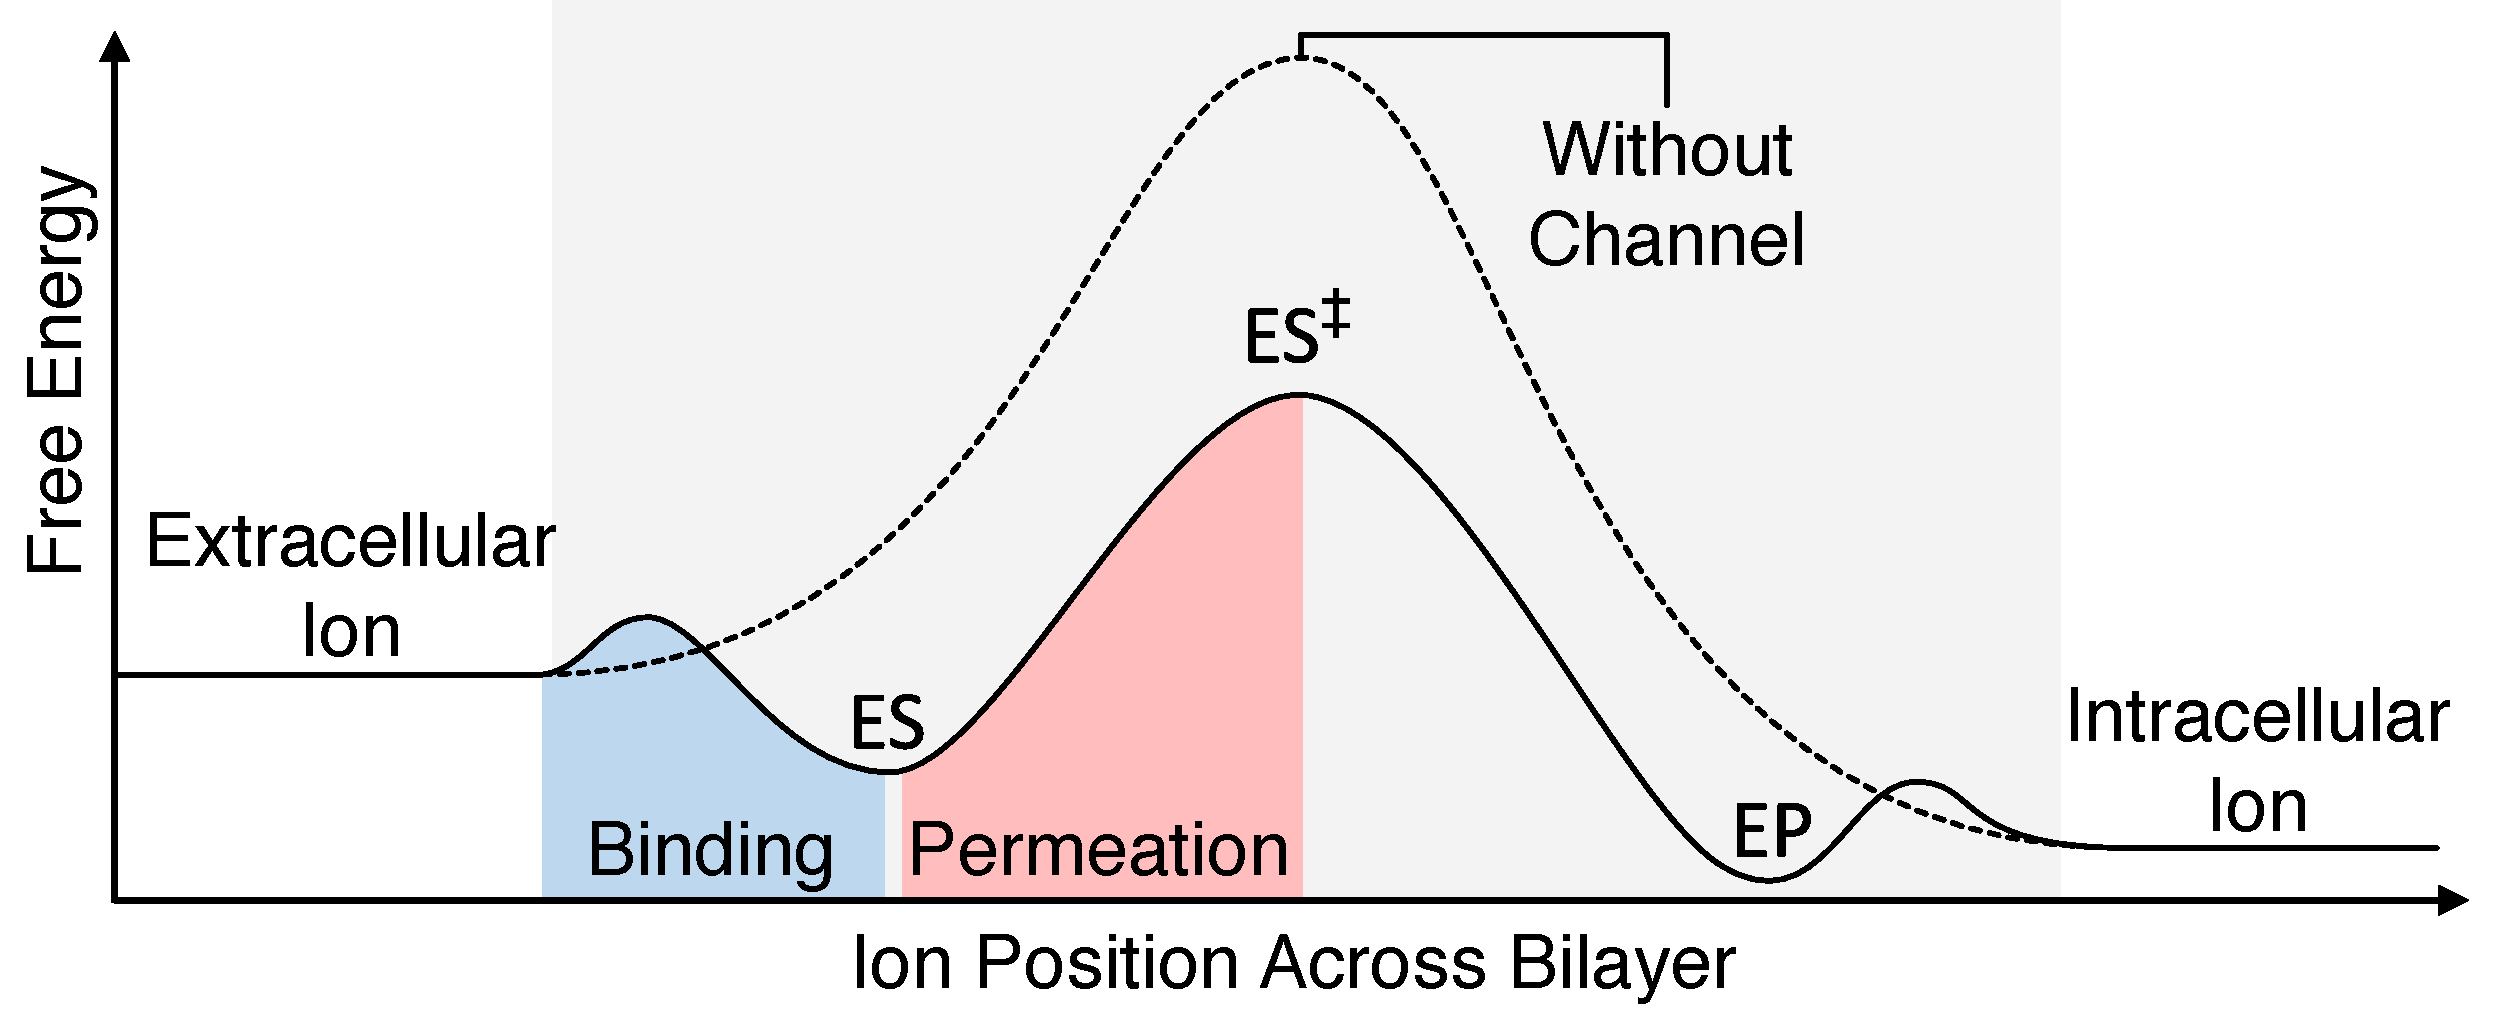
\includegraphics[width=0.6\textwidth]{introduction/enzyme}
\caption[Ion channels are enzymes that catalyze ion conduction]{\textbf{Ion channels are enzymes that catalyze ion conduction}. Schematic diagram depicts the free energy of substrate translocation along a reaction coordinate, with (black solid line) and without (black dashed line) catalysis by an enzyme. Here the reaction coordinate refers to the movement of an ion across a bilayer (grey shaded region) which is catalyzed by an ion channel. Enzyme and substrate ``reactions'' are arbitrarily separated into binding (blue) and permeation (red) events in the terminology of ion conduction.}
\label{fig:enzyme}
\end{figure}

Channels are efficient, permitting ion translocation at a rate of ~10$^6$ ions per second, faster than alternative transport mechanisms like transporters or carriers by several orders of magnitude and faster than turnover rates for well-studied enzymes like trypsin and pepsin \cite{Andersen:1992tf}. Ion channels are capable of operating near the diffusion limit, whereby the translocation rate is restricted by the time it takes for an ion to diffuse through the solvent to the channel opening \cite{Andersen:1983bl}. Once a sufficient number of ions have entered the channel, ion-ion repulsion can assist in the translocation of ions faster than diffusion rate. By nature of their intrinsic charge, ions prefer a polar environment, preferably surrounded by a shell of water molecules. Rapid movement through the confines of a channel can be achieved by maintaining a polar environment for permeating ions. As it can be observed in crystallographic structures of metalloproteins, metals like sodium and potassium preferentially bind to pockets of polar ligands, often in active sites of enzymes. Many of the same design principles hold in ion channels, with the caveat that ions cannot be bound too tightly, or else they may block the channel. More generally, the mechanism of catalysis results from a multitude of energetic contributions that may differ considerably between different families of channels. 

Catalysis by channels depends strongly on the chemical nature of the substrate. Ion channels may range from completely non-selective, allowing any ion of sufficient size to pass, to highly selective, allowing only one ion type to enter. The ions with highest concentration in human cells are Na$^+$, K$^+$, Ca$^{2+}$, and Cl-, which differ in atomic weight, formal charge, and effective radius \cite{Hille:2001tw}. The effective ionic radii are 1.02, 1.38, and 1.00 \AA\ for Na$^+$, K$^+$, and Ca$^{2+}$, respectively \cite{Shannon:1976dq}. Despite having different charges, Na$^+$ and Ca$^{2+}$ have a similar radius, suggesting that Na$^+$ and Ca$^{2+}$ selective channels may share some common features. By contrast, although Ca$^{2+}$ and K$^+$ have similar atomic weights, K$^+$ has a larger spread of electron density due to its monovalent charge which results in a qualitatively larger radius than both Ca$^{2+}$ and Na$^+$. Characterization of ions by effective radii enables the estimation of ion binding sites, but it does not provide information about how strongly they bind. The amount of free energy required to transfer a mole of ions from vacuum to a volume of water is called the hydration free energy. The experimental Gibbs free energy of hydration for Na$^+$, K$^+$, and Ca$^{2+}$ are -365, -295, -1505 kJ mol $^{-1}$, respectively \cite{Marcus:1991kp}. Na$^+$ has a lower hydration free energy than K$^+$, suggesting that it forms moderately stronger interactions with water molecules. The divalent charge of Ca$^{2+}$ strongly polarizes surrounding water molecules resulting in strong interactions. Both the ionic radius and hydration free energy are two of many factors that channels may evolve to accommodate in order to achieve selectivity. The mechanism by which channels are selective is poorly understood.

The passage of ions through channels commonly occurs through a pore formed by the assembly of multiple protein tertiary or quaternary structure elements. Some pores remain constitutively open, while others can open and close in response to a stimulus, like mechanical stretch, ligand binding, pH, ionic concentration, temperature, and voltage \cite{Zheng:2015vj}. These gating mechanisms provide a means for the cell to regulate the flow of substrates in and out of the cell and to ultimately achieve cellular homeostasis. For example, multiple transport proteins are involved in maintaining the optimal concentrations of water, ions and other molecules required for cellular processes to occur. In mammalian skeletal muscle, the extracellular ion concentrations of Na$^+$ and K$^+$ are 145 mM and 4 mM, while intracellular ion concentrations are 12 mM and 155 mM, respectively \cite{Hille:2001tw}. Two of several membrane proteins functioning to hold this concentration imbalance are voltage-gated Na$^+$ and K$^+$ channels (which by convention are denoted as Na\textsubscript{V} and Kv channels). These channels open and close in response to a difference in charge across the membrane. Gating can occur at any position within a channel pore, and may involve conformational change in one region or concerted motions of multiple subunits. All types of gating may halt the movement of substrates across the bilayer, and genetic mutations that alter gating are frequent causes of disease \cite{Ashcroft:2000ts}.

Permeation, selectivity, and gating are fundamental concepts that underlie the functional catalysis of substrates across biological membranes. A deeper understanding of these concepts will assist in improved treatment of patients suffering from defective ion channels and provides a foundation for rational design of channel directed therapeutics.
%One more big picture sentence?

\section{Physiological Role of Ion Channels and Disease}

Over billions of years, channels have evolved to match the growing complexity of cells, transporting diverse substrates under unique regulation mechanisms. Large-scale genome sequencing has provided a means to predict channel genes, driving researchers to clone, express, and functionally characterize many prokaryotic and eukaryotic channels. In human cells, the superfamily of voltage-gated ion channels has been identified and can be interpreted using evolutionary analysis (Fig. \ref{fig:channelome_ap} A) \cite{Yu:2004ep}. This family includes voltage-gated sodium, potassium, and calcium channels, as well as cyclic nucleotide-modulated channels, two-pore channels, and transient receptor potential channels. These channels are expressed in human cells throughout the body and serve diverse functions \cite{Zheng:2015vj,Hille:2001tw}. One of the most ancient of these functions originated shortly after multicellular life evolved, approximately 600 million years ago \cite{Chen:2014du}, enabling cell-to-cell communication and ultimately permitting the evolution of the nervous system.

\begin{figure}[hp]
\centering
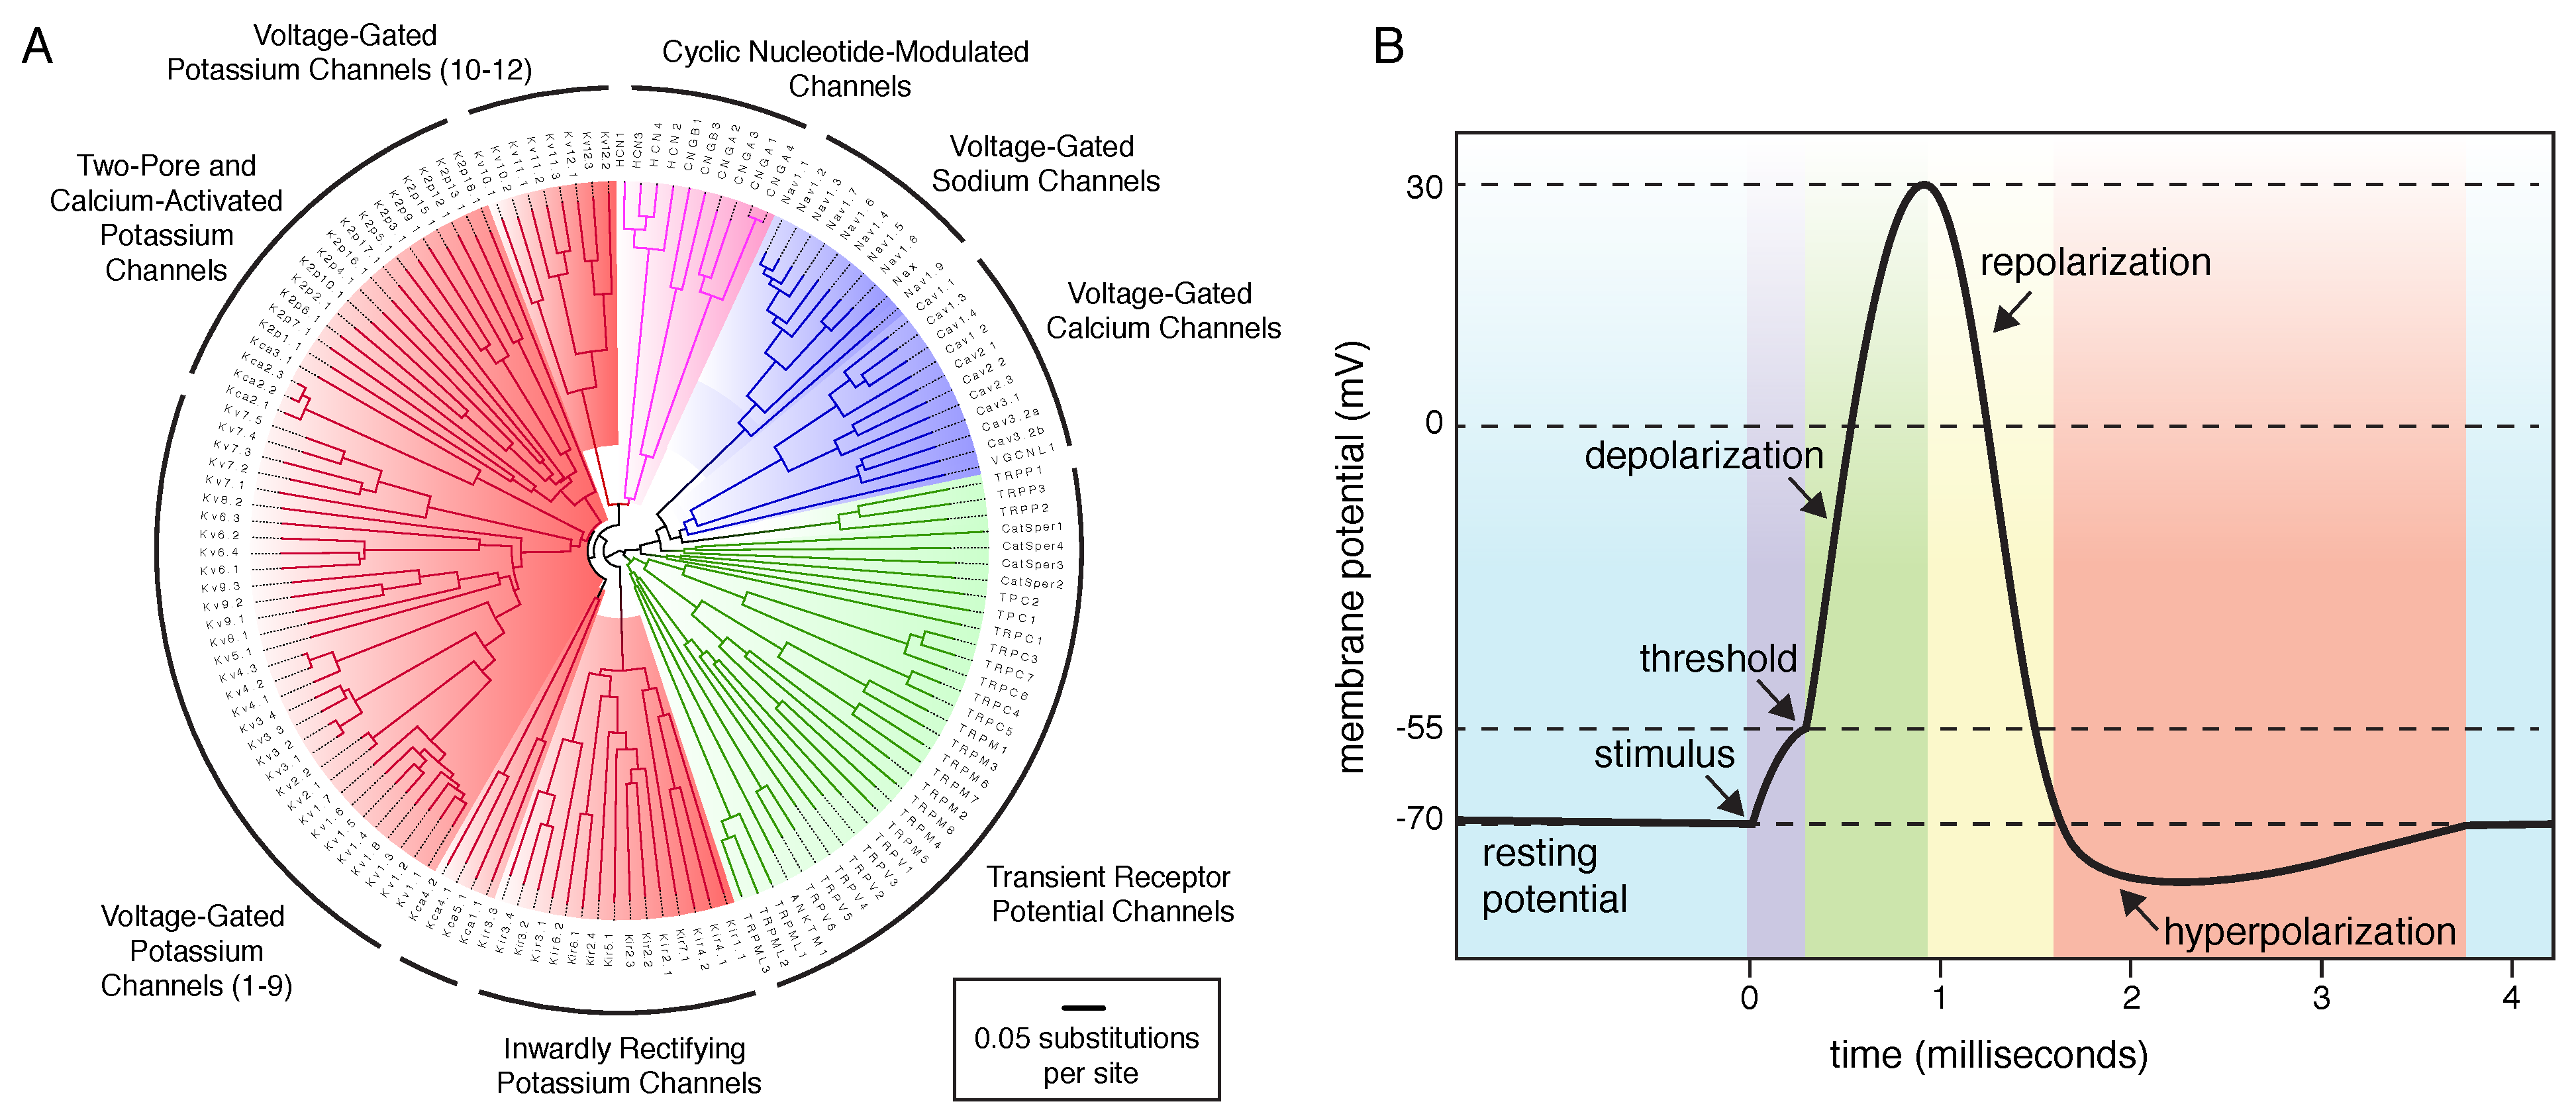
\includegraphics[width=0.9\textwidth]{introduction/channelome}
\caption[Phylogeny of voltage-gated ion channels and action potential schematic]{\textbf{Phylogeny of voltage-gated ion channels and action potential schematic}. (\textbf{A}) Phylogenetic tree of the voltage-gated ion channel superfamily present in the human genome. A set of amino acid sequences from the minimal pore regions of 142 voltage-gated ion channels were collected and sequence aligned \cite{Yu:2004ep}. A phylogenetic tree was constructed, without bootstrapping, using the BIONJ algorithm implemented in SplitsTree \cite{Gascuel:1997ua}. The tree was polarized and coloured using the software FigTree. Voltage-gated ion channel clades are labelled: potassium channels (red), cyclic nucleotide-modulated channels (pink),  sodium and calcium channels (blue), and transient receptor potential channels (green). (\textbf{B}) Schematic representation of an action potential. The course of the action potential is split into five phases; the resting phase (blue), the stimulus phase (purple), the depolarization phase (green), the repolarization phase (yellow), the refractory period (red), and back to the resting phase (blue). Sodium channels and potassium channels are predominately open during the depolarization and repolarization phase, respectively.}
\label{fig:channelome_ap}
\end{figure}

Voltage-gated sodium channels (Na\textsubscript{V} channels) were first characterized by Hodgkin and Huxley in a series of landmark papers published in 1952 \cite{Hodgkin:1952td,Hodgkin:1952vd,Hodgkin:1952um,Hodgkin:1952uf,Hodgkin:1952tr}.  Using the voltage-clamp technique on the membrane of the squid giant axon, Hodgkin and Huxley were able to describe complex phenomena in sodium channels such as voltage-dependent activation, fast inactivation, and Na$^+$ selectivity over other ions. In excitable cells, like neurons, muscle cells, and endocrine cells, Nav and Kv channels result in fast and transient reversals of membrane potential called ``nerve impulses'' or ``action potentials'' in the order of 2-5 milliseconds \cite{Bezanilla:2008ht,Hille:2001tw,Catterall:2012cd}. In neurons, the action potential has a characteristic membrane voltage profile when examined as a function of time, and proceeds sequentially through the following steps (Fig. \ref{fig:channelome_ap} B):
\begin{itemize}
\item \textbf{Stimulus}. An excitatory postsynaptic channel or an action potential from a nearby region causes a localized depolarization of the membrane from its resting state (-70 mV). Many failed activations may occur before the membrane voltage reaches a critical threshold of -44 mV.
\item \textbf{Depolarization}. Once the voltage threshold is reached, Na\textsubscript{V} channel opening probability increases. In the presence of open channels, a difference in ion concentrations and asymmetry of charge across the membrane drives ions through the pores. This driving force is called the electrochemical gradient. While Na$^+$ flows through open Na\textsubscript{V} channels, the membrane becomes even more depolarized, and triggers a positive feedback loop that causes nearby Na\textsubscript{V} channels to open. The highest Na$^+$ currents occur near a membrane potential of 0 mV.
\item \textbf{Repolarization}. At such depolarizing voltages, Kv channels opening probability increases. Open Kv channels permit K$^+$ to flow down its electrochemical gradient to outside of the cell. Outflow of K$^+$ repolarizes the membrane causing Na$^+$ channels to inactivate and subsequently close.
\item \textbf{Undershoot}. As the membrane potential approaches its resting state, some K$^+$ channels close, but prolonged opening causes polarization beyond the resting membrane potential, referred to as hyperpolarization.
\item \textbf{Refractory Period}. After a prolonged interval, the resting membrane potential is gradually restored at the site of interest (-70 mV). During this time, inactivated Na\textsubscript{V} channels cannot be made to activate at any membrane potential. The self-propagating nature of this mechanism drives the action potential to traverse the length of the neuron, and the refractory period helps ensure that the action potential will not move backwards.  
\end{itemize}

Action potentials play a vital role in human physiology. In neurons, this process permits long-distance signalling in the nervous system. In cardiac and skeletal muscle cells, action potentials play a critical role in muscle contraction. In pancreatic $\beta$ cells, the action potential stimulates the release of insulin. At the molecular level, these critical physiological processes rely on selective transport of ions, and thus it is not surprising that impairment of sodium flux through Na\textsubscript{V} channels can result in devastating human diseases. Mutations in the genes encoding for human Na$^+$ channels can result in diseases broadly classified as epileptic/non-epileptic, muscle, or pain disorders \cite{Ashcroft:2000ts}. Epileptic and non-epileptic disorders range from generalized epilepsy with febrile seizures (GEFS+) and Dravet syndrome to familial hemiplegic migraine and autism. Muscle disorders include hyper- and hypo- kalemic periodic paralysis, long QT syndrome (abnormal repolarization of the heart), along with paramyotonia congenita (prolonged muscle contraction). Pain disorders include congenital insensitivity to pain, and paraoxysmal extreme pain disorder. Na\textsubscript{V} channels have also been identified as serving non-canonical roles in non-excitable cells like astrocytes, T cells, macrophages, and cancer cells \cite{Black:2013gp}. In bacteria, prokaryotic Na\textsubscript{V} channels function to maintain sodium ion concentration and pH homeostatis \cite{Ito:2004da}, but may serve additional functions that are not understood.

The central physiological role of Na\textsubscript{V} channels position them as important drug targets. Human sodium channels are blocked by drugs used clinically as local anesthetics, antiarrythmics, and antiepileptics \cite{Catterall:2014eq}. In several drug binding sites, eukaryotic and prokaryotic Na\textsubscript{V} channels have very similar pharmacological characteristics. Electrophysiological studies reveal that the local anesthetics lidocaine \cite{Lee:2012bs}, isoflurane \cite{Ouyang:2007he}, and sevoflurane \cite{Barber:2014us}, can inhibit the bacterial sodium channel NaChBac in a similar manner to eukaryotic Na\textsubscript{V} channels. Functional electrophysiological studies reveal that the prokaryotic channel Na\textsubscript{V}Ms binds and is inhibited by small hydrophobic sodium channel blockers in a similar manner to human Nav1.1 \cite{Bagneris:2014ks}. Tested channel blockers include the clinically relevant lamotrigine and lidocaine, commonly used anticonvulsant and anesthetic drugs, respectively. Similarly, functional and structural characterization reveals that the prokaryotic calcium channel Ca\textsubscript{V}Ab is blocked by human Cav1.2 channel inhibitors \cite{Tang:2016el}. Given the pharmacological similarity of eukaryotic and prokaryotic Na\textsubscript{V} channels, recent structural determination efforts focused on prokaryotic channels provide a useful basis for understanding human Na\textsubscript{V} channel related diseases and designing therapeutics.

\section{Voltage-gated Ion Channel Structure and Function}

In 1971, before any ion channel sequence or structure was determined, Hille was able to construct a structural model of the narrowest constriction in Na\textsubscript{V} channels, the selectivity filter or SF, by measuring the permeability of a range of organic cations \cite{Hille:1972wz,Hille:1971vq}. Hille predicted a rectangular selectivity filter of dimensions 3 $\times$ 5 \AA\ that was lined with oxygen atoms, and predicted that permeating Na$^+$ could be partially hydrated and make direct contacts with up to three oxygen ligands of the selectivity filter.  In a follow-up study, Hille measured the permeability of a range of metal cations through sodium channels and found a characteristic ordering of selectivity (Na$^+$ $\approx$ Li$^+$ $>$ Tl$^+$ $>$ K$^+$ $>$ Ca$^{2+}$) \cite{Hille:1972wz,Eisenman:1962dy}. Based on the ``field strength'' theory of Eisenman \cite{Noda:1987gc,Eisenman:1983tc}, strong negatively charged ligands, like carboxyl oxygen atoms, could create ``high field'' binding sites for small cations preferentially, and Hille found that his results were consistent with this model. This work, along with many studies like it, laid the foundation for the structural investigation of ion permeation and selectivity in ion channels.

Cloning and expression of mammalian Na\textsubscript{V} channel led to the identification of a toxin binding site within the pore \cite{Noda:1986jn,Noda:1986ct,Terlau:1991ud,Noda:1989bj}. Through both mutagenesis and selectivity measurements for organic and inorganic cations, this site formed by a ring of residues with sequence ``DEKA'' was determined to be the selectivity filter \cite{Terlau:1991ud,Schlief:1996tb,Sun:1997uj}. Alignment of several calcium channel sequences revealed an ``EEEE'' ring at the same position within the putative calcium channel SF, and thus motivated site-directed mutagenesis to modify the eukaryotic sodium channel SF at this location \cite{Heinemann:1992ep}. The mutation of ``DEKA'' to ``DEEA'' or ``DEEE'' was sufficient to confer selectivity properties characteristic of a calcium channel, suggesting that this region alone is sufficient to impart selectivity. A mutation of the glutamic acid in ``DEKA'' to remove this high-field strength channel ligand was also found to decrease Na$^+$ selectivity over K$^+$ \cite{Favre:1996dg} in agreement with the Eisenman model. Conversely, subsequent experiments suggest the ``EEEE'' ring alone is sufficient to confer calcium selectivity in Cav channels \cite{Yang:1993ux,Ellinor:1995ky,Cibulsky:2000ix}, suggesting high structural homology between Nav and Cav channels. However, the distinction between Nav and Cav channels is often blurred across the kingdoms of life.

Phylogenetic analysis suggests that Na\textsubscript{V} channels evolved from Cav channels \cite{Hille:1989vz,Hille:2001tw,Yu:2004ep,Liebeskind:2011dn,GurBarzilai:2012kh} (Fig. \ref{fig:channelome_ap} A), but functional characterization of channels reveals greater complexity. The characteristic ``DEKA'' SF sequence is conserved in all vertebrate and many invertebrate Na\textsubscript{V} channels \cite{Widmark:2010in} and the ``EEEE'' and ``EEDD'' SF sequence are conserved in Cav1/Cav2 and Cav3 channels, respectively, in all known animal species back to the single-cell organisms which they originated \cite{Stephens:2015iv}. An evolutionary relationship between Cav and Na\textsubscript{V} channels is supported by putative "evolutionary intermediates" containing a ``DEEA'' SF sequence in several invertebrates. One of these channels, the German cockroach Na$^+$ channel 1 (BSC1), has high sequence similarity to Na\textsubscript{V} channels and is permeable to both Na$^+$ and Ca$^{2+}$ but could be functionally classified as a Cav channel \cite{Zhou:2004tc}. On the contrary, the \emph{Apis mellifera} Na\textsubscript{V} channel has the same ``DEEA'' motif, but is selective for Ca$^{2+}$ and impermeable to Na$^+$ \cite{GosselinBadaroudine:2016gw}, suggesting that regions outside of the SF influence selectivity. Indeed, modifications to residues in close vicinity to the SF were required to achieve Na$^+$ selectivity in a related invertebrate channel classified as a Na\textsubscript{V} channel \cite{GurBarzilai:2012kh}. Additionally, the evolutionary relationship between prokaryotic and eukaryotic Nav and Cav channels is unclear, however some studies suggest that eukaryotic sodium and calcium channels share prokaryotic sodium channels as a common ancestor \cite{Ren:2001uo,Yu:2004ep,Koishi:2004hy,Catterall:2015dh,Charalambous:2011dc}. The bacterial sodium channel NaChBac and several prokaryotic relatives were found to possess the same ``EEEE'' motif as observed in SF of Cav channels \cite{Ren:2001uo}. Bacterial sodium channels form homo-tetrameric assemblies of transmembrane helices S1-S6, whereas the mammalian Nav and Cav channels consist of a hetero-tetrameric assembly of a single chain containing 24 transmembrane helices \cite{Guy:1986bl,Ren:2001uo,Koishi:2004hy}. Mutagenesis studies reveal that the SF of prokaryotic Na\textsubscript{V} channels can be modified to impart Ca$^{2+}$ selectivity by introducing multiple ``DDDD'' rings within the SF \cite{Tang:2014cn,Shaya:2011ih,Yue:2002ee}. As such, bacterial voltage-gated sodium channels offer an promising model for gaining an understanding of the principles of Na$^+$ permeation and selectivity in the larger sodium and calcium channel superfamily.

% Thinking about full-on director's commentary in the comments of my thesis. (This negative result took 5000 CPU years, Reviewers ate us alive on this,) 

\subsection{Voltage-gated Ion Channel Structures}

% Explain features of Na\textsubscript{V}Ab, 
Sixty years after the seminal work of Hodgkin and Huxley, the first three-dimensional structure of a bacterial voltage-gated sodium channel, Na\textsubscript{V}Ab, was solved by x-ray crystallography \cite{Payandeh:2012ib,Catterall:2012fh}. The structure of Na\textsubscript{V}Ab consists of four identical subunits, each contributing one pore domain monomer and one voltage sensing domain (Fig. \ref{fig:nav_sf} A, extracellular view). All of the pore domain monomers, each comprised of transmembrane helices S5 and S6, form the ion conduction pore along the principal axis of the channel. Permeating sodium ions flow down their electrochemical gradient from the extracellular to intracellular side of the membrane, passing through several regions of the pore (Fig. \ref{fig:nav_sf} C, side view). Ions are first recruited to the pore entrance by negatively charged residues in the extracellular vestibule (EC). Past this point, ions enter through the narrowest constriction of the pore, named the selectivity filter (SF). The SF and surrounding features of the EC, comprised by pore helix P1 and P2, contribute the primary structural determinants for Na$^+$ selectivity. Beyond the SF, ions enter a water-filled expansion within the channel, named the central cavity (CC). Below the CC at the intracellular end of the pore, is another narrow constriction called the activation/intracellular gate (AG/IC). This constriction is formed by close packing of S6 helices when the pore domain is in a closed state, and dilates to some extent in the open state. Each subunit of the central pore domain is connected to a voltage-sensing domain, comprised of transmembrane helices S1-S4, by a structured S4-S5 linker. In Na\textsubscript{V}Ab and all known bacterial Nav structures, the voltage-sensing domains are ``domain-swapped'', making contact with the pore domain of the neighbouring pore domain monomer. Upon membrane depolarization, S4 transmembrane helices undergo conformational change which is translated to the intracellular gate of the pore domain through rearrangement of S6 helix packing \cite{Vargas:2012ek,Long:2005hl,Jensen:2012ee,Catterall:2015dh}. 

% Quick paragraph on K$^+$ channel stuctures
Nav and Kv channels share a similar domain architecture with a central pore domain and four voltage sensing domains (Fig. \ref{fig:nav_sf} A-D). The first crystallographic structure of a K$^+$ channel, KcsA, was solved more than a decade before the sodium channel structure \cite{Doyle:1998wq}. Building on the work of this landmark paper, structures from multiple families of K$^+$ channels represented in the phylogeny of human voltage-gated ion channels have now been solved (Fig. \ref{fig:channelome_ap} A) \cite{Tian:2013er,Kuang:2015jn}. This includes structures of several voltage-gated potassium channels [KvAP \cite{Jiang:2003vh}, Kv1.2 \cite{Long:2005do}, the Kv1.2/Kv2.1 chimera (Fig. \ref{fig:nav_sf} B,D) \cite{Long:2007cv}, and KvLm \cite{Santos:2012gg}]. Kv channels of known structure have similar overall architecture to bacterial Na\textsubscript{V} channels but differ considerably in the SF (Fig. \ref{fig:nav_sf} B).

\begin{figure}[hp]
\centering
\includegraphics[width=0.9\textwidth]{introduction/navsf}
\caption[Molecular rendering of voltage-gated ion channels and selectivity filter structure of Na$^+$ and K$^+$ selective channels]{\textbf{Molecular rendering of voltage-gated ion channels and selectivity filter structure of Na$^+$ and K$^+$ selective channels}. Molecular snapshots of the tetrameric assembly of (\textbf{A}) sodium channel Na\textsubscript{V}Ab \cite{Payandeh:2012ib} and (B) a potassium channel chimera, Kv1.2/Kv2.1 \cite{Long:2007cv} from the extracellular view. (\textbf{C-D}) Snapshots of Na\textsubscript{V}Ab and Kv1.2/Kv2.1 channels embedded in a lipid bilayer after coarse-grained molecular dynamics \cite{Stansfeld:2015tb}. Only two of four subunits are depicted from a side-orientation to assist in visualizing the protein interior. Lipid molecules are shown in white and water molecules in red and white. Cylinders depict the helices forming the voltage-sensing domain (helices S1-S4, orange), the S4-S5 linker (blue), pore- domain helix S5 (red), the pore helix (purple), and pore-domain helix S6 (yellow). Na\textsubscript{V}Ab contains an additional helix near the selectivity filter (green). A dashed box indicates the position of the selectivity filter. Molecular renderings of two opposite subunits of the selectivity filter in (\textbf{E}) Na\textsubscript{V}Ab \cite{Payandeh:2012ib} and (\textbf{F}) KcsA \cite{Zhou:2001vo}. Residue numbers are shown for pore-lining channel ligands. Within the SF, each label indicates an observed or putative ion binding site.}
\label{fig:nav_sf}
\end{figure}

\begin{figure}[hp]
\centering
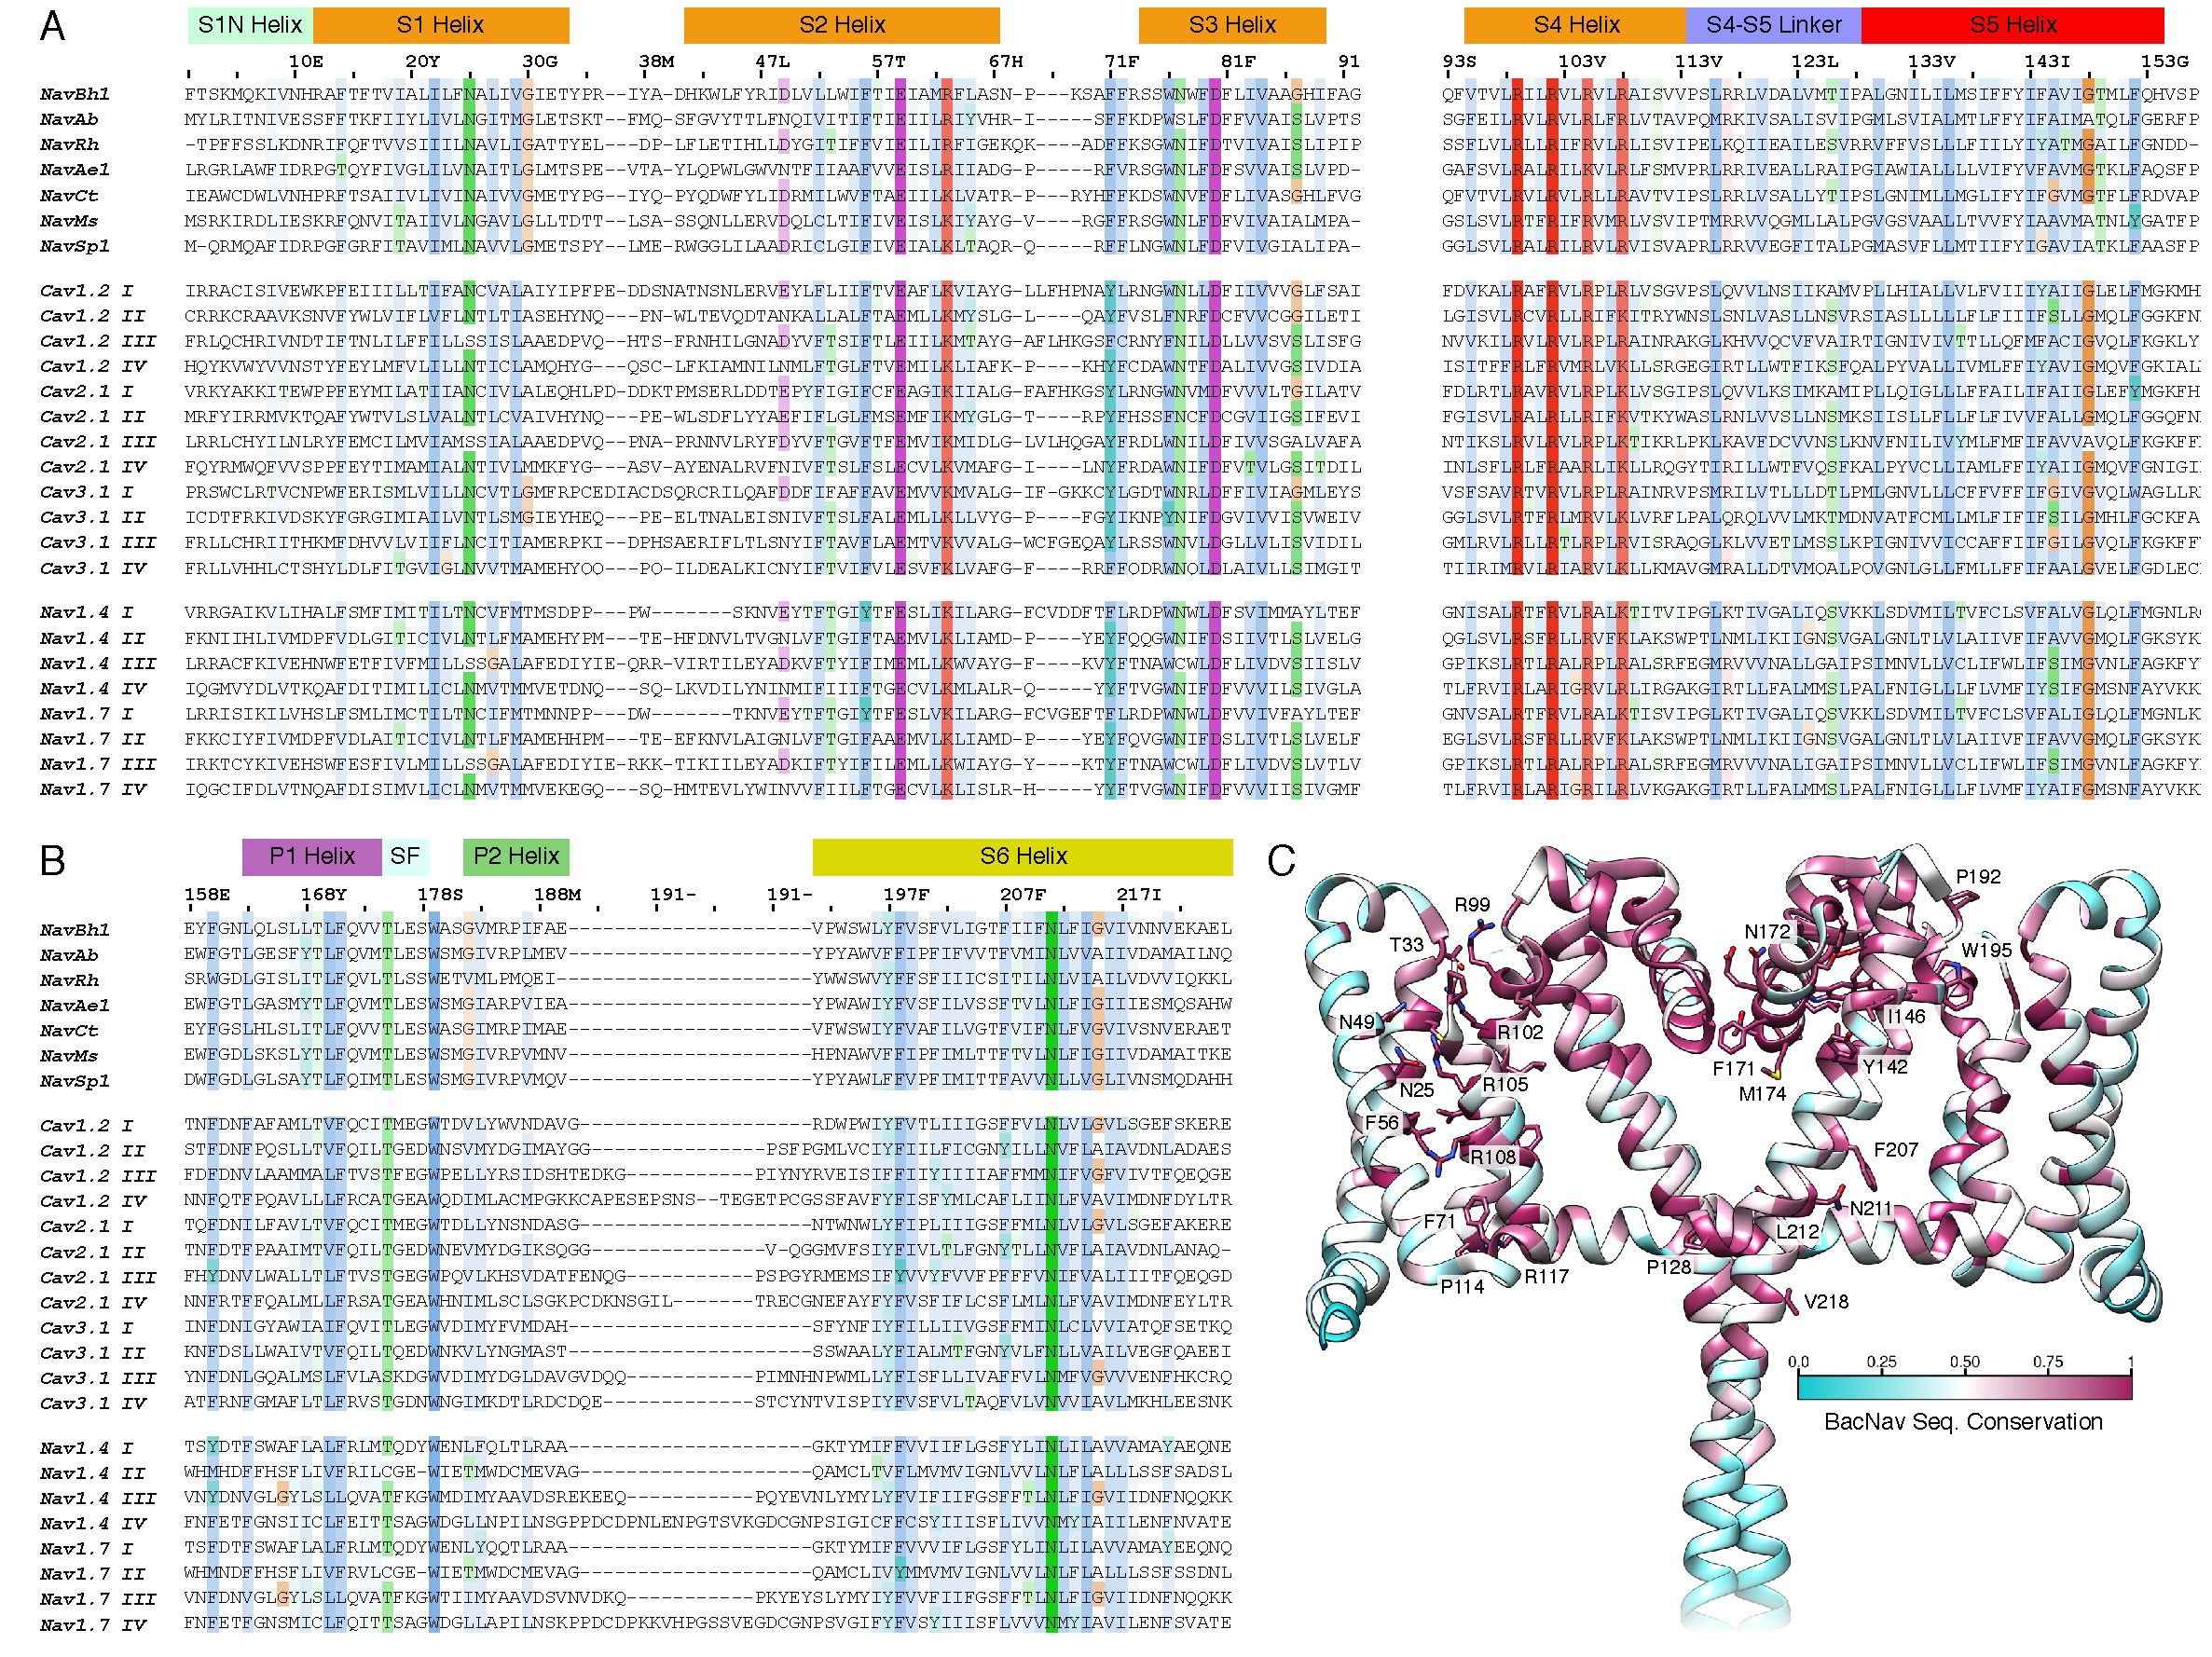
\includegraphics[width=1.0\textwidth]{introduction/sequence}
\caption[Voltage-gated sodium and calcium channel sequence alignment and conservation]{\textbf{Voltage-gated sodium and calcium channel sequence alignment and conservation}. Sequence alignment of structurally and functionally characterized homo-tetrameric prokaryotic sodium channels along with multiple heterotetrameric human Nav and Cav channels. (\textbf{A}) Sequence alignment is shown using Na\textsubscript{V}Ab as a reference for both the numbering and secondary structure assignments of the (\textbf{A}) S1-S5 and (\textbf{B}) P1-S6 helices. (\textbf{C}) A molecular rendering of two diagonal subunits from the full-length Na\textsubscript{V}Ab/FY structure \cite{Lenaeus:2017cy} colored by sequence conservation across three hundred bacterial Na\textsubscript{V} channel homologs. Sequence conservation was calculated using the ConSurf web server \cite{Landau:2005de}. Selected residues with greater than 90\% conservation in the dataset were labelled and colored in purple.}
\label{fig:sequence}
\end{figure}

\subsection{Voltage-gated Ion Channel Selectivity Filters}

% K$^+$ channel SF
The SF of K$^+$ channels is narrow and lined exclusively with backbone carbonyl groups \cite{Doyle:1998wq,Long:2005do,Long:2007cv}. Electron density assigned to K$^+$ ions were localized within the SF of K$^+$ channels in high-resolution crystal structures \cite{Zhou:2001vo}. These data suggest that K$^+$ occupies four sites within the K$^+$ channel SF which are formed by cages of eight carbonyl groups that directly coordinate the ions (S1-S4), as well as one additional site (S0) lying outside of the SF (Fig. \ref{fig:nav_sf} F). As K$^+$ moves through the channel from the intracellular to extracellular side of the membrane, the narrow radius of the SF requires that equatorial water molecules be stripped from its solvation shell. The free energy penalty of a dehydrated K$^+$ ion is partially compensated by direct contacts with channel ligands. This mechanism for ion binding and permeation is thought to confer high selectivity of K$^+$ channels against Na$^+$ \cite{Nimigean:2011ww}, often quoted as high as 1000:1 selective for K$^+$ over Na$^+$, the molecular basis for K$^+$ selectivity is still debated in the literature \cite{Andersen:2011ty}.

% Na\textsubscript{V} channel SF second, because it flows better
The sequence of each of the four loops making up the SF in bacterial channels Na\textsubscript{V}Ab \cite{Payandeh:2012ib}, Na\textsubscript{V}Ms \cite{McCusker:2012di,Naylor:2016cu,Bagneris:2013bu,Sula:2017hu} and Na\textsubscript{V}Ae \cite{Shaya:2014gg,Arrigoni:2016fs}, is ``TLES'' (Fig. \ref{fig:nav_sf} E, Fig. \ref{fig:sequence} B). This region contains the selective ``EEEE'' ring. The Na\textsubscript{V} channel SF is shorter and wider than that of the prototypical K$^+$ channel SF (Fig. \ref{fig:nav_sf} F) \cite{Doyle:1998wq} and is wide enough to accommodate partially or even fully hydrated Na$^+$ ions, in agreement with Hille's prediction \cite{Hille:1971vq,Payandeh:2012ib}. Relative ionic currents through Na\textsubscript{V}Ab indicate that this channel is only weakly selective for Na$^+$ over K$^+$ by a ratio of 10:1 \cite{Payandeh:2012ib}. Bound cations were not observed in any Na\textsubscript{V}Ab structure \cite{Payandeh:2013ex,Payandeh:2012ib,Lenaeus:2017cy}. Channel ligands that coordinate permeating cations in the lumen of the SF include the backbone carbonyl groups of residues T175 and L176 (in the residue numbering of Na\textsubscript{V}Ab), as well as the carboxylate and hydroxyl groups of the side chains of residues E177 and S178, respectively. The SF of Na\textsubscript{V}Ab is wide enough to accommodate a fully hydrated sodium ion based on its approximate effective radius \cite{Payandeh:2012ib}. Although no electron density attributed to Na$^+$ was found within the SF of this structure, the existence of binding sites could be inferred based on the geometry of channel ligands. In accord with the high-field-strength model of Eisenman \cite{Eisenman:1983tc}, it was posited that Na$^+$ ions would exchange some of the water molecules in their first solvation shell with carboxylate oxygen atoms of E177 at a site referred to as SHFS \cite{Payandeh:2012ib}. Upon deeper entry of Na$^+$ into the SF, the ion is suggested to become fully hydrated at a site centrally coordinated by backbone carbonyls of L176 at a site referred to as SCEN. Finally, ions may also become coordinated to T175 at a site referred to as SIN before entering the central cavity. These three sites (SHFS, SCEN, SIN) were inferred based on the static structure of the Na\textsubscript{V}Ab SF, but additional experimental evidence in other bacterial Na\textsubscript{V} channels supports binding at these approximate locations. Three highly occupied Na$^+$ binding sites were observed in the SF of two homologous Na\textsubscript{V}Ms structures \cite{Naylor:2016cu,Sula:2017hu}. All three binding sites were identified on the central axis of the channel, with positions that correspond to SHFS site, a site slightly above SCEN, and a site slightly above SIN, respectively. From these observed binding sites, the authors infer that Na$^+$ remains fully hydrated as it permeates the SF. In addition, on-axis Ca$^{2+}$ binding sites were identified, likely fully hydrated, above SHFS and at SCEN/SIN in Na\textsubscript{V}Ae \cite{Shaya:2014gg} and Na\textsubscript{V}Rh structures \cite{Zhang:2013bz}, respectively. Electron density provides useful experimental support for ion binding sites, but it does not provide sufficient information to infer an ion permeation mechanism in the physiological state of the channel, necessitating additional studies.

Eukaryotic voltage-gated Ca$^{2+}$ channels possess the same characteristic ``EEEE'' ring shown to impart Na$^+$ selectivity in the SF of bacterial Na\textsubscript{V} channels. The structural features responsible for this inversion of selectivity are not known, despite new structural data. A 3.6 \AA\ resolution cryo-EM structure of the rabbit Cav1.1 channel did not have high enough resolution to accurately resolve the side chain orientations within the SF \cite{Wu:2015bb} (Fig. \ref{fig:navstructures} L). In accordance with earlier studies demonstrating that the Na\textsubscript{V} channel SF could be modified to impart Ca$^{2+}$ selectivity by introducing rings of ``DDDD'', high resolution crystal structures of these mutants were obtained \cite{Tang:2014cn,Catterall:2015dh}. The high-resolution crystallographic structure of these mutants revealed there was only minor changes in backbone geometry of the SF compared to Na\textsubscript{V}Ab (Fig. \ref{fig:navstructures} J).  Together, these studies suggest that selectivity is governed predominately by side chain interactions in this channel rather than the backbone geometry of the SF per se.  Based on electron density within the selectivity filter of crystallographic structures obtained with Ca$^{2+}$ in the crystallization medium, three binding sites were identified on the central axis of the channel, implying that Ca$^{2+}$ is bound in a hydrated form.  While this work supports a mechanism for Ca$^{2+}$ conduction based on structural evidence, it does not isolate the energetic factors that govern Ca$^{2+}$ selectivity, or provide an explanation for Na$^+$ selectivity over Ca$^{2+}$ in Na\textsubscript{V}Ab. 

\subsection{Classification of Sodium Channel Structures}

Functional characterization through electrophysiology has been performed on twelve bacterial Na\textsubscript{V} channels, which show a broad range of activation and inactivation gating properties \cite{T:2014eg,Payandeh:2015hz}. The functional diversity of these channels suggests that structural investigation, even lacking voltage control in crystallization conditions, should be sufficient to obtain structures spanning the closed-open-inactive state cycle \cite{Amaral:2012tn,Bagneris:2014eh,Sula:2017jx}. Structures of bacterial Na\textsubscript{V} channels were obtained in closed [Na\textsubscript{V}Ab \cite{Payandeh:2012ib}, Na\textsubscript{V}Ae \cite{Shaya:2014gg,Arrigoni:2016fs}, and Na\textsubscript{V}Ct \cite{Tsai:2013ie}], inactivated [Na\textsubscript{V}Ab \cite{Payandeh:2013ex} and Na\textsubscript{V}Rh \cite{Zhang:2013bz}], and open [Na\textsubscript{V}Ab \cite{Lenaeus:2017cy} and Na\textsubscript{V}Ms \cite{McCusker:2012di,Bagneris:2014ks,Naylor:2016cu,Sula:2017hu}] states (summarized in Fig. \ref{fig:navstructures} and Table \ref{table:navs}). Sequence alignment and conservation analysis reveals high homology between these structures (Fig. \ref{fig:sequence}). The classification of structures into these states is performed on the basis of the conformations of the voltage-sensing domains (activated or inactivated), the conformation of the selectivity filter (open or closed/collapsed), and the intracellular gate (open or closed). It is hypothesized that all prokaryotic channels sample these states as the channel moves through a closed-open-inactive state cycle \cite{Amaral:2012tn,Bagneris:2014eh,Sula:2017jx}. In the closed state of Na\textsubscript{V}Ab, the SF is wide enough to permit a sodium ion but the intracellular/activation gate is closed. The structure of Na\textsubscript{V}Ab has also been solved with both open and closed intracellular gates and the conformational of the SF remains the same \cite{Lenaeus:2017cy}. However, structures of both Na$^+$ and K$^+$ channels have been solved with the SF in an inactivated state, impermeable to ions \cite{Zhou:2001vo,Zhang:2013bz,Payandeh:2013ex}. In the K$^+$ channel KcsA, the conformation of the intracellular gate is coupled to the SF \cite{Cuello:2010gi,Kratochvil:2017ge,Cuello:2010kf}, and structures have been obtained with its intracellular gate sampling a wide range of diameters. It is not known if a similar type of intracellular gate coupling to the SF is observed in Na\textsubscript{V} channels. Nonetheless, the similarity between the open and closed conformations of the Na\textsubscript{V}Ab SF, and homologous bacterial Na\textsubscript{V} channel SFs, motivates its use as a sufficient model for studying ion conduction and selectivity in a major functional state of the channel. 

When the membrane is depolarized, the voltage sensor undergoes a conformational change from a resting state to an activated state, causing the pore domain to open and permit ion conduction. All known Na\textsubscript{V} channel structures have voltage sensors that are hypothesized to be in the activated state, showing only minor variations in the orientation of side chains. The state of the voltage sensors are classified based on the translation of the helix S4 and its conserved arginine sidechains \cite{Vargas:2012ek}. Specifically, the movement of these arginine sidechains are measured with respect a conserved phenylalanine in the hydrophobic constriction of the voltage sensor (F56 of helix S2, in Na\textsubscript{V}Ab). In the activated structure of the Na\textsubscript{V} channel VSD, three (R1 to R3) or four (R1 to R4) of the arginine sidechains are facing the extracellular side of the hydrophobic constriction \cite{Payandeh:2012ib,Zhang:2013bz}. In the resting structure of the two-pore potassium channel TPC1, S4 translation was observed and no arginine sidechains were oriented above the hydrophobic constriction \cite{Guo:2016jb}. Heterogeneous conformations of the voltage-sensing domains were observed in the eukaryotic channels NavPaS and EeNav1.4 \cite{Yan:2017kd}. Comparison of these VSD structures results in a model for the electromechanical basis involving a iris-like pore domain dilation conferred through the S4-S5 linker by lateral displacement and upward translation of the S4 helix \cite{Yan:2017kd,Shen:2017df}. Voltage sensors may also undergo rotation with respect to the pore domain, as observed when comparing NavPaS and EeNav1.4, Na\textsubscript{V}Rh and Na\textsubscript{V}Ab \cite{Payandeh:2015hz,Zhang:2013jf}, and in simulations of Kv channels \cite{Jensen:2012ee}. However, recent structures of tetrameric channels homologous to voltage-gated ion channels reveal a loss of the domain-swapped tetrameric arrangement of the pore-domain and VSD, and in some cases the loss of a structured S4-S5 linker entirely, suggesting that voltage-gating may involve a more complex mechanism in some channels \cite{Wang:2017kg,Whicher:2016ix,Lee:2017ix,Hite:2017kh,Li:2017ex,Tomczak:2017gf}. 

Several pore-only Na\textsubscript{V} channel constructs, with truncated voltage-sensing domains, have been utilized to obtain crystal structures of the first open Na\textsubscript{V} channel and first Na\textsubscript{V} channel with a resolved C-terminal domain \cite{Shaya:2014gg,McCusker:2012di}. Constructs lacking voltage-sensing domains form stable tetrameric assemblies that undergo opening and closing transitions permitting selective ion flux \cite{Shaya:2011ih,McCusker:2011tn}. Prokaryotic Na\textsubscript{V} channels possess an intracellular coiled-coil domain, resolved in several crystal structures (Fig. \ref{fig:navstructures} D,I-K). The upper region of the coiled-coil domain can adopt a partially disordered structure, based on electron paramagnetic resonance spectroscopy and the full-length Na\textsubscript{V}Ms structure \cite{Bagneris:2013bu,Sula:2017hu}, as well an ordered helical structure \cite{Lenaeus:2017cy,Tang:2014cn,Arrigoni:2016fs,Shaya:2014gg}. Despite low sequence homology in the coiled-coil region (Fig. \ref{fig:sequence} C), this domain is important for channel assembly and gating \cite{Mio:2010cb,Bagneris:2013bu,Powl:2010ke,Irie:2012dn,Tsai:2013ie,Shaya:2014gg,Arrigoni:2016fs}. Although multiple high-resolution structures of Na\textsubscript{V} channels exist, it is difficult to assert that these structures are truly representative of the functional open, closed, and inactivated states of the channel, warranting additional experimental and computational studies.

% One more sentence?

\begin{figure}[hp]
\includegraphics[width=1.0\textwidth]{introduction/navstructures}
\caption[Voltage-gated sodium and calcium channel structures]{\textbf{Voltage-gated sodium and calcium channel structures}. Prokaryotic sodium channels [Na\textsubscript{V}Ab (\textbf{A}, \textbf{B}, \textbf{F}, \textbf{I}), Na\textsubscript{V}Ms (\textbf{C}, \textbf{G}, \textbf{K}), Na\textsubscript{V}Ae1p (\textbf{D}), and Na\textsubscript{V}Rh (\textbf{E})], a putative eukaryotic sodium channel [Na\textsubscript{V}PaS (\textbf{H})], and calcium channels [Ca\textsubscript{V}Ab (\textbf{J}), Ca\textsubscript{V}1.1 (\textbf{L})] are shown from the side orientation. Molecular visualizations of two opposite subunits within the tetrameric complex coloured according to common structural elements in each channel. Structural elements are voltage sensing domains (S1-S4 helix, orange), S4-S5 linker (blue), S5 helix (red), pore helix 1 and 2 (purple and green, respectively), S6 helix (yellow), coiled-coil domain (cyan, only in prokaryotic channels), intracellular and extracellular domains (pink and black, respectively, only in eukaryotic channels). Channel names are followed by the year of publication and the putative state of the channel with the protein databank code and structural resolution in brackets.}
\label{fig:navstructures}
\centering
\end{figure}

\begin{table}[h!]
\centering
\renewcommand{\arraystretch}{1.5}
\begin{tabular}{lllllllll}
  \topline
  \headcol Name & PDB & SF & VSD & IC Gate & CTD & SF Ions & I$_{Na^+}$ & Ref. \\
  \midline
   Na\textsubscript{V}Ab/I217C & 3RVY & open & activated & closed & not resolved & no & yes & \cite{Payandeh:2012ib}\\
   Na\textsubscript{V}Ab & 4EKW & closed & activated & closed & not resolved & no & yes & \cite{Payandeh:2013ex}\\
   Na\textsubscript{V}Ab/1-226 & 5VB8 & open & activated & open & truncated & no & yes & \cite{Lenaeus:2017cy}\\
   Na\textsubscript{V}Ab/FY & 5VB2 & open & activated & closed & coiled-coil & no & no & \cite{Lenaeus:2017cy}\\
  \rowcol Na\textsubscript{V}Ms & 4F4L & open & removed & pre-open & not resolved & Na$^+$ & yes & \cite{McCusker:2012di}\\
  \rowcol & 3ZJZ & open & removed & open & not resolved & Na$^+$ & yes & \cite{Bagneris:2013bu}\\
  \rowcol & 5HVX & open & activated & open & interaction & Na$^+$ & yes & \cite{Sula:2017hu}\\
  \rowcol Na\textsubscript{V}Ms/E177D & 4X88 & open & removed & open & not resolved & Na$^+$ & yes & \cite{Naylor:2016cu}\\
  Na\textsubscript{V}Ae & 4LTO & open & removed & closed & coiled-coil & Ca$^{2+}$ & no & \cite{Shaya:2014gg}\\
  & 5HK7 & open & removed & closed & coiled-coil & Na$^+$ & no & \cite{Arrigoni:2016fs}\\
  \rowcol Na\textsubscript{V}Rh/G208S & 4DXW & closed & activated & closed & not resolved & Ca$^{2+}$ & no & \cite{Zhang:2013bz}\\
  Na\textsubscript{V}Ct & 4BGN & open & activated & closed & S6 ext. & no & yes & \cite{Tsai:2013ie}\\
  & 4BGN & open & activated & open & S6 ext. & no & yes & \cite{Tsai:2013ie}\\
  \rowcol Na\textsubscript{V}PaS & 5XOM & open & activated & closed & resolved & no & no & \cite{Shen:2017df}\\
  EeNa\textsubscript{V}1.4 & 5XSY & open & activated & open & resolved & no & yes & \cite{Yan:2017kd}\\
  \rowcol Ca\textsubscript{V}1.1 & 5GJV & open & activated & closed & resolved & Ca$^{2+}$ & N/A & \cite{Wu:2015bb}\\
  Ca\textsubscript{V}Ab/DDD & 5KLB & open & activated & closed & resolved & Ca$^{2+}$ & N/A & \cite{Tang:2014cn}\\
  \bottomlinec
\end{tabular}
\caption[Na\textsubscript{V}/Ca\textsubscript{V} channel structural and functional descriptions]{\textbf{Na\textsubscript{V}/Ca\textsubscript{V} channel structural and functional descriptions}. Structural components and functional properties of each channel are described qualitatively. Name refers to the channel shorthand name, typically `Na\textsubscript{V}' or `Ca\textsubscript{V}' followed by an abbreviation of the organism name, along with any mutations that were introduced into the construct. For each structure, PDB refers to the protein databank identifier, SF/VSD/IC Gate/CTD refer to the state of the structural element, SF ions refers to the presence of electron density associated with ions resolved in the SF of each structure, I$_{Na^+}$ refers to measured currents of Na$^+$ in the construct, and Ref. refers to the article providing more information on each structure.}
\label{table:navs}
\end{table}

\section{Molecular Mechanisms of Permeation and Selectivity}

Ion conduction and selectivity are processes governed by the underlying physics of ions and their interaction with water and channel ligands. The confined environment of a channel pore results in several factors contributing to ion permeation and selectivity, which may be broadly classified as ion-protein, ion-water, ion-ion, and protein-protein interactions. The extent to which each of these factors plays a role in ion conduction and selectivity in different channels cannot be accurately estimated a priori, and necessitates combined experimental and computational studies.

The conductance of ion channels can be directly measured in the lab using voltage clamp techniques \cite{Hille:2001tw,Sakmann:1984cc}. These technique enabled the measurement of single channel currents conducted through single purified sodium channels in phospholipid bilayers. Na$^+$ and K$^+$ conductance ($\gamma$) was 25.2 and 3.5 picosiemens (pS), respectively in the rat brain sodium channels \cite{Hartshorne:1985tk}. Using Ohm's Law, $i=\gamma V_m$, at a membrane potential of +100 mV, this would correspond to currents of 2.52 and 0.35 picoamperes of current (or $2.5 \times 10^6$ and $3.5 \times 10^5$ ions/sec). By taking the ratio of these conductances, $3.5/25.2=0.14$, we can arrive at the permeability or selectivity of the channel. In this work, we represent selectivity as a ratio of Na$^+$ over K$^+$, in this case by $7.2:1$. Selectivity can also be computed experimentally in several other ways: the reversal potential for currents under bi-ionic conditions \cite{Hille:2001tw}, crystallographic titration \cite{Sauer:2013gk,Alam:2009bu,Liu:2013hf}, or through channel block experiments \cite{Neyton:1988wj,Neyton:1988vv,Nimigean:2002fp}. The selectivity of ion channels can also be obtained computationally from: the ratio of ion conductance \cite{Sotomayor:2007ej,Kutzner:2011fz}, by free-energy perturbation \cite{Kim:2011eg,Noskov:2004tv}, or by comparing the potential of mean force (PMF) for the permeation of different ion species \cite{Nimigean:2011ww,Roux:2011ed}. A PMF describes the free energy required for a biophysical process to occur, averaging over all other degrees of freedom in our simulation. For example, in this work we frequently compute the PMF for ion movement along the principal channel axis, averaging over any protein or water fluctuations (Fig. \ref{fig:enzyme}). In a PMF or free energy profile of ion permeation, ion binding affinity is reflected by free-energy well depth (free energy in the bulk - free energy at ES, in Fig. \ref{fig:enzyme}) and permeation rates can be correlated with the height of free energy barriers (ES$\cross$, in Fig. \ref{fig:enzyme}), which together may be used to estimate selectivity when ions are compared. 

Computational approaches for calculating conductance and selectivity can provide dynamic information about these processes at high resolution and temporal accuracy, something few experimental techniques can achieve. As ions enter the channel pore, the energetic cost of ion and pore desolvation must be compensated by favorable ion-protein interactions which must be weak enough to prevent bound ions from blocking permeation \cite{Roux:2011ed,Alam:2011ud}.  A long-standing mechanism of K$^+$ channel permeation called ``knock-on'' was hypothesized by Hodgkin and Keynes in 1955 \cite{Hodgkin:1955hu} and later observed in computer simulations \cite{Berneche:2003ua,Berneche:2001un}. In this mechanism, the entry of K$^+$ into an SF occupied by multiple single-file K$^+$ ions causes the simultaneous exit of a K$^+$ on the opposite side of the SF through ion-ion repulsion. K$^+$ permeation is now widely accepted to occur through a knock-on mechanism \cite{Domene:2003tn,Jensen:2010fd,Aqvist:2000eo,Roux:2005kd}. The details of water-ion cotranslation in this process have been called into question in a study emphasizing the destabilizing role of direct contacts between permeating cations in achieving a rate of K$^+$ permeation approaching the diffusion limit \cite{Kopfer:2014cj}, but 2D IR spectroscopy experiments do not support this model \cite{Kratochvil:2016jx}. Qualitatively, the mechanism of K$^+$ permeation in K$^+$ channels is well studied and agreed upon, but the mechanism for K$^+$ selectivity is more uncertain.

Experimental and computational studies have led to several selectivity mechanisms for K$^+$ channels \cite{Andersen:2011ty,Roux:2017bs}. The ``snug-fit'' model of selectivity suggests that the SF primarily distinguishes ions based on ionic radius. In this model, an optimal distance from a bound K$^+$ to cages of channel ligands would result in ion selectivity, and conduction occurs through electrostatic repulsion between ions \cite{Mullins:1960tn,Bezanilla:1972uz}.  However, this model was unable to reconcile the measurement that thermal fluctuations of the SF were larger than the difference between the ionic radius of Na$^+$ and K$^+$ \cite{Noskov:2004tv}, supporting a model of ion selectivity emphasizing the interplay of attractive ion-ligand interactions and repulsive ligand-ligand interactions in a dynamic pore interior \cite{Noskov:2006fd}. Several models support the hypothesis that flexible binding sites may impart selectivity by virtue of the physicochemical properties of channel ligands \cite{Yu:2010dj,Varma:2007ws,Dixit:2009fo}. Subsequent simulation-based models of K$^+$ channel selectivity rely on both thermodynamic and kinetic factors \cite{Kim:2011eg,Thompson:2009ig}. In addition to playing a critical role in facilitating ion conduction through the ``knock-on'' mechanism, multi-ion effects were found to play a role in selectivity as well \cite{Ye:2010hs,Derebe:2011jc,Sauer:2011ky}. The importance of kinetic factors is evident in studies of the NaK channel, where electrophysiological measurements of two single-point mutants, one of which was found to be selective and the other non-selective despite both channels being reported as K$^+$ selective over Na$^+$ at equilibrium \cite{Liu:2013hf,Sauer:2013gk}. Although these studies further our understanding of K$^+$ channels and provide plausible models for K$^+$ selectivity, there is little consensus on the general mechanism of selectivity for K$^+$ channels. Given the different architecture of the Na\textsubscript{V} channel SF, the extent to which models of selectivity based on studies of K$^+$ channels apply to Na\textsubscript{V} channels is not established.

%However, the availability of multiple voltage-gated sodium channel structures makes it possible to refine mechanistic hypotheses about ion permeation and selectivity which were originally proposed for K$^+$ channels.

%Computer simulations of ion channels may be used to identify the molecular driving forces for ion binding, permeation, and selectivity.  In order to study these concepts, a simulation methodology must be selected that establishes a channel model, a force field, a sampling algorithm, and the extent of sampling.  The accuracy of simulation results depends heavily on these methodological choices due to a combination of both systematic and statistical errors.  Statistical errors refer to limitations due to insufficient data set sizes, whereas systematic errors reflect biases resulting not only from inherent limitations of the force field and of the channel model, as well as from the simulation protocol itself.  Sampling errors include both statistical and systematic errors.  Systematic sampling errors arise from imperfect initial conditions, which incur a need for equilibration of the system, and from rare conformational transitions due to ?hidden? or unforeseen energy barriers, which can make equilibration exceed the time of the simulations \cite{Neale:2013fw}.  Before discussing simulation results, in this section we provide an overview of the methods utilized in computational studies of Na\textsubscript{V} channels (see Table XXXXXXX) and comment briefly on their relationship to simulation error.

\section{Thesis Contributions and Organization}

%Numerous studies have examined the molecular basis for Na$^+$ conduction and selectivity in Na\textsubscript{V} channels.

The focus of this dissertation is to examine the molecular structure and function of bacterial voltage-gated sodium channels. Using computational techniques, this body of work provides novel insights into the mechanistic details of Na\textsubscript{V} channel function. In particular, we examine three overarching concepts of ion channels; permeation, selectivity, and gating, as well as the molecular basis of pathogenic mutations.

More specifically, the main research contributions of this thesis are:
\begin{itemize}
\item a detailed investigation of the molecular basis for Na$^+$ and K$^+$ conduction,
\item a model describing the molecular basis for Na$^+$ over K$^+$ selectivity in the wildtype and mutant channels, 
\item an experimentally testable hypothesis regarding the relationship between channel fluctuations and ion conduction and selectivity,
\item an examination of hydrophobic gating in the intracellular gate of an open-state channel,
\item insight into the molecular basis of hypokalemic periodic paralysis caused by ionic currents through mutant voltage sensing domains.
\end{itemize}

In this chapter we presented an overview of voltage-gated ion channel physiology and structure, providing necessary context for our subsequent studies on the bacterial voltage-gated sodium channel. The modelling and simulation protocols common to multiple research projects in this work are presented in Chapter 2. In Chapters 3 to 6, we examine the atomistic details of ion conduction and selectivity through the narrowest constriction of the pore, the SF. In Chapter 7, we examine how ion conduction proceeds beyond the SF, at the intracellular gate, in open and closed channels. In Chapter 8, we examine how malfunctioning voltage sensing domains, periphery to the central pore domain, result in leaky pores, ultimately resulting in disease. Finally, in Chapter 9, we review the primary findings of this thesis and provide an outlook for future studies of voltage-gated sodium channels.

Methodological issues related to the choice of force field and model construction are described in Appendix A and B, which provide technical justification for the simulation protocols utilized in Chapters 3 to 8. 

\printbibliography[heading=subbibnumbered,title={References}]
%\printbibliography[heading=subbibliography]
\end{refsection}
 \begin{refsection}
 \chapter{Methodology}

Multiple biophysical methods have been developed to investigate the molecular structure and function of membrane proteins \cite{Cournia:2015df,PebayPeyroula:2008wv}. Structural determination of membrane proteins can be achieved using x-ray crystallography, cryo-electron microscopy, or solid-state NMR \cite{Lacapere:2010fl}. With a sufficient amount of structural data, homology modelling and other bioinformatics algorithms can be utilized for membrane protein structure prediction but require careful validation \cite{Almeida:2017kq,Stansfeld:2017dk}. Protein structures are not required, but provide a concrete foundation for further biochemical and biophysical studies. Using a membrane protein activity assay, be that through electrophysiological techniques \cite{Rettinger:2016uc} or some other functional assay, it is possible to probe the molecular structure and function relationship using site-directed mutagenesis, drug-binding, or other environmental perturbations. Further quantification of membrane protein function can be determined using biophysical techniques. Circular dichroism spectroscopy can provide secondary structure information \cite{Miles:2016ks}, and fourier transform infrared spectroscopy can provide high-sensitivity measurements of conformational change \cite{Tatulian:2013hy}. Both F\"{o}rster resonance energy transfer \cite{Loura:2011ig} and and electron paramagnetic resonance \cite{Sahu:2015kd} can provide distance information between two specific sites, another effective tool to study conformational change in membrane proteins. Analytical ultracentrifugation \cite{Fleming:2016hi}, surface plasmon resonance \cite{Patching:2014bg}, atomic force microscopy \cite{Whited:2014hb}, and mass spectrometry \cite{Landreh:2014fs} serve as invaluable tools for investigating membrane protein assembly and other molecular interactions. The dynamics of proteins can be investigated at atomic resolution using serial femtosecond crystallography \cite{Zhu:2016cp} or molecular dynamics simulations \cite{Dror:2012cs,Chavent:2016cq}. Each of these approaches holds strengths and weaknesses, varying in their technical requirements, temporal, and spatial resolution. The selection of these methods is largely dependent on the timescale of the biological process of interest.

The action potential rises and falls over a few seconds. During this time, voltage-sensing domains cause sodium channels to open and ion permeation occurs. Conduction measurements for a typical voltage gated sodium channel are on the order of one sodium permeation event per microsecond \cite{Hille:2001tw}. To study the dynamics of this process, we require a method that has both atomic resolution as well as fine temporal resolution that can span up to one or more microseconds. Recent developments in high-performance computing hardware and computational algorithms have enabled the use of all-atom molecular dynamics simulations to study biological processes over a large range of timescales, from femtoseconds to microseconds (corresponding to 9 orders of magnitude). Simulations have been utilized extensively for the study of ion conduction and selectivity, and led to major discoveries in the molecular mechanism of ion permeation and selectivity \cite{Dror:2010gy}. In this chapter, we describe the methods used throughout this thesis in order to investigate the structure and function of voltage-gated sodium channels.

\section{Statistical Mechanics}

Molecular dynamics simulations are part of a group of computational methods that can be utilized to generate ensembles of atomic configurations for the calculation of macroscopic properties. We define a configuration, or microstate, as a fixed set of positions and momenta for $N$ atoms. The collection of microstates form a macrostate. For example, we might define the open state and closed state of an ion channel as two separate macrostates. The configurations accessible for a system depend on global variables held constant and define a thermodynamic ensemble. Constant variables may include the number of particles ($N$), volume ($V$), temperature ($T$), or pressure ($P$). Experimental studies are typically conducted in the canonical ensemble ($N$,$V$, and $T$ held constant) or the isothermal-isobaric ensemble ($N$,$P$, and $T$ held constant) so simulations typically employ the same approaches. The probability of finding a configuration $P_i$ is related to the total energy of the system at that microstate, $E_i$, normalized by the sum of all microstates,

\begin{equation}
\label{eq:1}
P_i = \frac{ \exp \big[ - \frac{E_{i}}{k_B T}\big]  }{  \sum_{j} \exp \big[ - \frac{E_{j}}{k_B T} \big]  }
\end{equation}

where $T$, the temperature, and $k_B$, a Boltzmann constant with units of $energy/temperature$, define a thermodynamic energy scale. This equation applies only to the canonical ensemble but a similar expression exists to describe the probability of a microstate being found in the isothermal-isobaric ensensemble. Microstates with energies higher than $k_B T$ are relatively inaccessible, with low population, and those with energies lower than $k_B T$ are more accessible and have a higher population. The total energy is a sum of the potential energy and kinetic energy at a given configuration, $E_{i}=U_{i}+K_{i}$. The denominator of equation \ref{eq:1} is the partition function. This quantity is the sum of exponential factors for each of the microstates available to the system, and specifies how microstates are partitioned into energy levels. These energy levels include the ground state energy, $E_0$, which is zero for simulations of classical systems. Here we consider a thermodynamic system with countable microstates, but for a physical system there are an infinite number of microstates and the summations in this expression and others in this section can also be written as integrals over all atom positions and momenta. The relationship between the number of accessible states and the temperature can be understood by examining the partition function in limiting cases. In the limit of low temperature, all exponential terms except for the ground-state energy term go to zero, resulting in occupancy of only a single microstate. At very high temperatures, all terms in the partition function approach $1.0$, resulting in the accessibility of all microstates. The ratio of probabilities of two microstates $i$ and $j$ correspond to their differences in their energies,

\begin{equation}
\label{eq:2}
\begin{split}
\frac{P_i}{P_j} & = \frac{ \exp \big[ - \frac{E_{i}}{k_B T}\big]  }{  \exp \big[ - \frac{E_{j}}{k_B T}\big]   } \\
                       & = \exp \Big[ - \frac{(E_{i} - E_{j})}{k_B T}\Big], \\
\end{split}
\end{equation}

which does not require the explicit calculation of a partition function. Similarly, the ratio of probabilities of two macrostates can be computed by dividing the sum of microstate probabilities within each macrostate. When the partition function is known, it can be utilized as weighting factors for the calculation of thermodynamic averages over all microstates within a macrostate. For example, the average energy $\langle E \rangle$ of a system at a given temperature is

\begin{equation} 
\label{eq:2a}
\begin{split}
 \langle E \rangle & = \sum_i E_i P_i \\
                            & = \frac{ \sum_{i} E_{i} \exp \big[ - \frac{E_{i}}{k_B T} \big]  }{  \sum_{j} \exp \big[ - \frac{E_{j}}{k_B T} \big]  }. \\
\end{split}
\end{equation}

A similar expression can be derived to calculate the thermal average of any observable. It is also possible to evaluate thermodynamic averages over a macrostate using a reduced partition function, containing a subset of microstates. Using the principles of statistical mechanics, it is possible to calculate both static equilibrium properties and dynamic or non-equilibrium properties. In the context of ion channels, examples of equilibrium properties include the ionic occupancy of binding sites and the spatial distribution of water within the pore. An example of a kinetic property is the rate of ion conduction, but this requires a time average rather than a thermodynamic average. Equilibrium properties are related to the calculation of free energy. The Helmholtz free energy (measured in the $NVT$ ensemble), $F$, and the Gibbs free energy (measured in the $NPT$ ensemble), $G$, can be computed from a partition function. In both statistical ensembles, this quantity represents the amount of work that can be obtained from the system. For a macrostate comprised of many microstates $i$,

\begin{equation}
F_i = - k_B T \ln \Big( \sum_{i} \exp \big[ - \frac{E_{i}}{k_B T} \big]  \Big).
\end{equation}

The logarithm of exponential factors is intrinsically related to free energy and can be utilized to compute differences in free energy without explicit calculation of the partition function. The difference in free energy, $\Delta F$ between macrostates $i$ and $j$ is 

\begin{equation}
\begin{split}
\Delta F & = F_i - F_j \\
              & =  -k_B T \ln \Big( \sum_{i} \exp \big[ - \frac{E_{i}}{k_B T} \big]  \Big) + k_B T \ln \Big( \sum_{j} \exp \big[ - \frac{E_{j}}{k_B T} \big]  \Big)\\
              & = -k_B T \ln \Big( \frac{\sum_{i} \exp \big[ - \frac{E_{i}}{k_B T} \big]}{\sum_{j} \exp \big[ - \frac{E_{j}}{k_B T} \big]}                         \Big) \\ 
              & = -k_B T \ln \Big( \frac{P_i}{P_j} \Big),
\end{split}
\end{equation}

where the last simplification is made using Eq. \ref{eq:1}. Free energies are utilized extensively to examine biophysical processes, but in practice, they are difficult to interpret due to their high dimensionality. In a continuous configurational integral over positions and momenta states, it is possible to project the distribution onto a lower-dimensional set of coordinates to gain greater biological insight \cite{Zuckerman:2010ue}. This is referred to as a potential of mean force (PMF, $W$) since it includes the average of all forces experienced by a particle except those on a specific reaction coordinate. The potential of mean force along a coordinate like distance, $R$, using a configurational integral over all positions and momenta ($\mathbf{r}^N$, $\mathbf{p}^N$) can be expressed as 

\begin{equation}
\label{eq:2b}
\begin{split}
 \exp \Big[ - \frac{W(R)}{k_B T} \Big] & = \frac{\int d\mathbf{r}^N d\mathbf{p}^N \delta \big( R - \hat{R}(\mathbf{r}^N) \big) \exp \big[ - \frac{E(\mathbf{r}^N, \mathbf{p}^N)}{k_B T} \big]}{\int d\mathbf{r}^N d\mathbf{p}^N \exp \big[ - \frac{E(\mathbf{r}^N, \mathbf{p}^N)}{k_B T} \big]} \\
                                                              & = P(R) \\
 \end{split}
\end{equation}

where $(\hat R)$ is a function that takes all coordinates and returns $R$, and the delta function, $\delta$, selects the positions and momenta associated with the coordinate $R$ out of the integral. $P(R)$ is a continuous probability distribution analogous to the single microstate expression given in equation \ref{eq:1}. An approximation of the PMF can be obtained, up to a constant $C$, by making a discrete estimation of $P(R)$ using a histogram of $R$ values, with the following expression,

\begin{equation}
\label{eq:3}
 W(R) = - k_{B}T \ln \big( P(R) \big) + C.
\end{equation}

In practice, the number of states and their corresponding energies cannot be simply enumerated for a complex system, so these quantities, including $P(R)$, cannot be exactly calculated. It is for this reason that the PMF is estimated relative to some reference point $R_0$, which sets the value of C. To enable numerical approximations of these values, we assume the average behaviour of an $N$-particle system can be studied by computing the time evolution of that system for a sufficiently long time and averaging over the quantity of interest. This assumption, called the ``ergodic hypothesis'', is correct when it is known that all states within a thermodynamic ensemble are accessible over long timescales. In practice, it is reasonable to assume that over finite-time simulations, all states will not be reached, but that a reasonable approximation can still be made for the calculation of observables. 

\section{Molecular Dynamics}

The objective of molecular dynamics simulations is to produce time trajectories of $N$ atoms which are guided by physical principles. With full treatment of atomic nuclei and electrons, the time evolution of $N$ atoms can be obtained by solving the time-dependent Schr\"{o}dinger equation. However, this equation can only be solved analytically for the hydrogen atom and even high-accuracy numerical methods are prohibitively expensive for multi-atom systems (with computational scaling on the order of O($M^{7}$) where $M$ is the number of basis functions)\cite{Jensen:2007wr}. As such, we use approximate models that are designed to reproduce a subset of quantum mechanical and experimental properties through parameterization of a potential energy function. Approximate models do not treat electronic degrees of freedom, and atoms are modelled as point masses with fixed charge. In addition, we make the assumption that quantum effects are negligible and that the motion of atoms can be predicted using classical physics. The time evolution of an atomic system containing $N$ interacting atoms can be described by Newton's equations. This collection of atoms forms a system of differential equations, and with a set of initial positions and momenta, it is possible to propagate the positions of atoms in type using numerical integration. Contrary to alternative sampling methods like Monte Carlo, consecutive configurations obtained from molecular dynamics are obtained using physical principles, which enables the calculation of kinetic properties.

In order to propagate the movement of atoms in time under Newton's laws, it is required to calculate the forces acting on each of $N$ atoms in the system. Forces are obtained from the gradient of the potential energy function $U$, or force field, which is comprised of both bonded and non-bonded energy terms. The CHARMM potential energy function \cite{MacKerell:1998tp}, used extensively in this work, has the form

\begin{equation}
\label{eq:4}
\begin{split}
U & = \sum_{bonds} K_b (b-b_0)^2 + \sum_{urey-bradley} K_{ub} (S-S_0)^2 + \\
    & \sum_{angles} K_{\phi} (\phi - \phi_0)^2 + \sum_{dihedrals} K_{\chi} (1+\cos(n\chi - \delta)) + \\
    & \sum_{impropers} K_{imp} (\psi - \psi_0)^2 + \sum_{lj_{i \neq j}} \epsilon_{ij} \Big[   \big(  \frac{R_{min_{ij}}}{r_{ij}} \big)^{12} - \big(  \frac{R_{min_{ij}}}{r_{ij}} \big)^{6}   \Big] + \sum_{coulomb} \frac{q_i q_j}{\epsilon_{eff} r_{ij}}, \\
\end{split}
\end{equation}

where $K_b$, $K_{ub}$, $K_{\phi}$, $K_{\chi}$, and $K_{imp}$ are empirical force constants; $b$, $S$, $\phi$, $\chi$, and $\psi$ are distance or angle variables for specific interactions, with subscript $0$ representing the equilibrium values for the terms. The first five summations indicate bonded energy terms which describe the local intramolecular interactions of biomolecules. The penultimate term defines the Lennard-Jones interactions, where $\epsilon_{ij}$ and $R_{min_{ij}}$ are the well depth and distance at the potential minimum, which includes a repulsive term at short-range and an attractive long-range term. The last contribution to the CHARMM potential energy is the Coulomb term, where $q_i$ and $q_j$ are the charges of two atoms $i$ and $j$ interacting at distance $r_{ij}$, and $\epsilon_{eff}$ is the effective dielectric constant. The last two terms of Eq. \ref{eq:4} are referred to as short-range and long-range non-bonded interactions. Since these interactions may be computed between any nearby atom of the simulation cell, not just those which are bonded, they are responsible for the most significant computational cost of molecular dynamics simulations. The functional form in Eq. \ref{eq:4} is fit using a broad range of experimental and \textit{ab initio} quantum mechanical data in order to produce a self-consistent set of parameters for proteins, water, ions, lipids, and other small molecules. The validation and improvement of force field parameterization of the CHARMM force field is an area of ongoing research \cite{Huang:2013ft,Huang:2016kb}. The calculation of forces between protein atoms and ions, critical to studies of ion channels, involves only non-bonded interactions. For example, when comparing the interaction of a sodium and potassium ions, both possessing a single positive charge, to a carboxylate oxygen atom at the same distance $r_{ij}$, the Coulombic energy term is equivalent, and the difference between these interaction are entirely determined by two parameters $R_{min_{ij}}$ and $\epsilon_{ij}$ in the calculation of the Lennard-Jones term. The optimization of these two parameters for sodium and potassium ions has been performed explicitly for the study of permeation and selectivity in ion channels \cite{Noskov:2008jp}. The potential form of equation \ref{eq:4} reveals another approximation of our molecular models; that assuming our simulations are conducted at a fixed $U$, no bonded terms can be modified, and thus no hydrogen bonds can be formed or broken. This approximation is acceptable for the study of ion channels, where no chemical bonds are broken during ion conduction. 

High-performance algorithms for molecular dynamics simulations are implemented in the software package GROMACS \cite{Abraham:2015gj,Hess:2008db,Pronk:2013ef}. This implementation includes a number of optimizations to assist in the calculation of non-bonded forces in periodic unit cells, rigid-body constraints, and support for arbitrary triclinic unit cells. GROMACS runs efficiently on GPUs as well as parallelized across hundreds of CPUs, which is essential for the simulation of membrane proteins, which may contain 100,000 or more atoms.

\section{Simulation Protocol}

A standard protocol is employed for all simulations of voltage-gated sodium channel presented in this work, and is commonly utilized within the molecular modelling and simulation community \cite{Kandt:2007wz}. This protocol proceeds though a series of steps that is performed manually, described in the following steps, but also through a similar process using the CHARMM-GUI Membrane Builder web service \cite{Wu:2014uc}: 
\begin{itemize}
\item \textbf{Membrane protein preparation}. We first construct the biological assembly of subunits that compose the entire membrane protein of interest. In the case of the voltage-gated sodium channel, a tetrameric biological assembly must be constructed, which is performed using the software CHIMERA \cite{Pettersen:2004kh}. All non-protein molecules are removed from the initial structure. Protein structures are frequently deposited into the protein databank with unresolved side chains or flexible loops. Homology modelling software is utilized to construct missing atoms and residues \cite{Fiser:2003we}. In the case of the voltage-gated sodium channel NavAb, no residues were missing within the TM region. All hydrogen atoms are added to the protein structure. N- and C-terminal groups are also constructed at the beginning and end of each peptide chain. When residues are missing from the N- and C-terminus, these residues are not explicitly modelled in our protocol. In the case of NavAb, the C-terminal domain of this protein was not resolved and these regions were not modelled. Neutral N- and C-terminal groups $-NH_2$ and $-COOH$ are added to assist in preserving the stability of the protein backbone, even though neutral termini are unphysical at physiological pH. Any single-point mutations to the structure are made using the software MODELLER at this point \cite{Fiser:2003we}. This membrane protein structure is then aligned with its principal axis along the Z-axis of the simulation cell by convention, with extracellular values positive and intracellular values negative with respect to the center of mass of the protein.
\item \textbf{Bilayer preparation}. A bilayer patch is obtained from an online repository, in a configuration after some simulation has been performed, or constructed using the CHARMM-GUI bilayer construction algorithm. In the latter case, relaxation of the simulation cell must be performed using independent molecular dynamics simulations. The size of the constructed bilayer varies depending on the size of the membrane protein construct. In the case of the voltage-gated sodium channel, we construct a rectangular bilayer patches with approximate X and Y dimensions of 83 \AA and 108 \AA for pore domain and full-length structures, respectively. It is standard practice to construct large bilayer patches with minimum periodic distance of at least twice the long-range cutoff. For some simulations of the full-length channel, we construct a bilayer patch within a truncated octahedron unit cell, which reduces the number of atoms in the box but does not necessarily decrease the distance of closest approach of the protein to its periodic image.
\item \textbf{Protein insertion into the bilayer}. Multiple algorithms exist to assist in the embedding of membrane proteins into bilayers. This process consists of removing overlapping lipid molecules, and assisting the packing of lipid molecules in the protein-lipid interface. For simulations of the voltage-gated sodium channel, we utilize $g\_membed$ \cite{Wolf:2010dr} and $alchembed$ \cite{Jefferys:2015jt} embedding protocols.
\item \textbf{Solvation and ionization}. Depending on the dimensions of the initial bilayer patch and protein embedding protocol, additional  water molecules may need be added to ensure that the protein is sufficiently solvated. There is no strong criteria for the selection of the height of the simulation cell used in our work. We do not model water molecules within the pore, but allow water molecules to enter the structure during the protein/water relaxation stage. The positions of water molecules are then exchanged for a specified concentration of NaCl, KCl, or a mixture of both. The number of ions inserted depends on the number of water molecules in the box, with a general target of 150 mM or 200 mM.
\item \textbf{Energy minimization}. After our membrane protein is inserted into a solvated lipid bilayer, steepest descent energy minimization performed with GROMACS\cite{Abraham:2015gj,Hess:2008db,Pronk:2013ef}  to remove unfavourable energy contacts that would normally cause molecular dynamics simulations to crash.
\item \textbf{System relaxation}. Initial simulations are performed with protein restraints that limit deviation away from the crystallographic structure. All simulations systems studied in this work are performed using GROMACS \cite{Abraham:2015gj,Hess:2008db,Pronk:2013ef} in the isothermal-isobaric ensemble, starting with three stages of relaxation, each lasting 10 ns. In these steps, harmonic position restraints were applied to heavy atoms, main chain backbone atoms, and then $C\alpha$ atoms, with a force constant of $1000 kJ mol^{-1} nm^{-2}$. The temperature and pressure of the simulation cell fluctuate around $300 K$ and $1 atm$, respectively. During this time, ions and water molecules flow into the channel pore and lipid molecules form closer contacts with the protein in the bilayer.
\item \textbf{Production simulations}. The final frame of system relaxation is utilized to create multiple simulation repeats. In some cases, multiple simulation repeats were conducted during the solvation and ionization stage. Each of the simulation repeats undergoes production simulations with GROMACS \cite{Abraham:2015gj,Hess:2008db,Pronk:2013ef} in the isothermal-isobaric ensemble. Data is analyzed across all simulation repeats.
\end{itemize}

\section{Umbrella Sampling}

The calculation of free energies is a foundational tool for the study of biomolecules using molecular simulation. In many cases, long timescale simulations permit the calculation of free energies along a defined order parameter, or reaction coordinate, which may assist in developing mechanistic conclusions about a biological process. In the study of ion channels, we employ this method to calculate the free energy of ion movement through the narrow confines of the channel selectivity filter using equation \ref{eq:3}. This technique works when the primary reaction coordinate and known orthogonal degrees of freedom are well-sampled over the timescale of simulations. For some channels, ions may move rapidly in and out of a well-hydrated region of the pore, resulting in reasonable estimates of free energy profiles. However, in partially or fully dehydrated region of the pore, the amount of energy required to move an ion through this constriction may require long timescale simulations, and spontaneous hydration of this region may be required before ion movement can occur. In this case, hydration and the conformation of pore lining side chains may be coupled to ion conduction, and need to be adequately sampled in order to obtain an accurate estimate of the free energy of ion conduction. The sampling of orthogonal degrees of freedom, like these, is a challenging problem for studying biological processes that occur at the temporal limits of modern simulation studies \cite{Neale:2016gj}. To assist in overcoming barriers along the reaction coordinate of interest, accelerating sampling techniques can be used. In the ``umbrella sampling'' method, an additional energy term, $U_{bias}$, is added to the total internal energy ($E=U+U_{bias}+K$) which enables the sampling of low population microstates along a reaction coordinate of interest \cite{Kastner:2011ft,Roux:1995js,Torrie:1977hs}. Enhanced sampling along a reaction coordinate $R$, is achieved by adding a harmonic biasing potential of the form

\begin{equation}
\label{eq:50}
U_{bias}(R) = \frac{1}{2} k (R-R_0)^2,
\end{equation}

where the strength of the harmonic spring is given by the force constant $k$, and the equilibrium value of the potential is placed at position $R_0$. This results in a modification to the potential energy which is similar to the addition of another bonded term in the force field. The unbiased expression for computing the probability distribution $P(R)$ is given by equation \ref{eq:2b}, and the biased expression is 

\begin{equation}
\label{eq:5}
\begin{split}
 P_{bias}(R) & = \frac{\int d\mathbf{r}^N \delta \big( R - \hat{R}(\mathbf{r}^N) \big) \exp \Big[ - \frac{U(\mathbf{r}^N) + U_{bias}(\hat{R}(\mathbf{r}^N))}{k_B T} \Big]}{\int d\mathbf{r}^N \exp \Big[ - \frac{U(\mathbf{r}^N) + U_{bias}(\hat{R}(\mathbf{r}^N))}{k_B T} \Big]} \\
                     & = \exp \Big( \frac{-U_{bias}(R)}{k_B T} \Big) \frac{\int d\mathbf{r}^N \delta \big( R - \hat{R}(\mathbf{r}^N) \big) \exp \Big[ - \frac{U(\mathbf{r}^N)}{k_B T} \Big]}{\int d\mathbf{r}^N d \exp \Big[ - \frac{U(\mathbf{r}^N) + U_{bias}(\mathbf{r}^N)}{k_B T} \Big]} \\
 \end{split}
\end{equation}

where the newly added biased potential is only dependent on $R$ in the numerator after the application of the $\delta$ function. For simplicity, here we do not include momentum in the definition of the microstate and thus we do not evaluate the kinetic energy term of the total internal energy. Combining this result with equation \ref{eq:2b} allows the unbiased probability $P(R)$ to be written as

\begin{equation}
\label{eq:5b}
\begin{split}
 P(R) & = P_{bias}(R) \times \exp \Big( \frac{U_{bias}(R)}{k_B T} \Big) \times \frac{\int d\mathbf{r}^N \exp \big[ - \frac{U(\mathbf{r}^N)}{k_B T} \big]  \exp \big[ - \frac{U_{bias}(R)}{k_B T} \big]   }{\int d\mathbf{r}^N \exp \big[ - \frac{U(\mathbf{r}^N)}{k_B T} \big]}   \\
         & = P_{bias}(R) \times \exp \Big( \frac{U_{bias}(R)}{k_B T} \Big) \times \langle \exp \big[ - \frac{U_{bias}(R)}{k_B T} \big] \rangle,  \\
 \end{split}
\end{equation}

where the thermodynamic average similar to equation \ref{eq:2a} was utilized to simplify the final term. This indicates that the unbiased probability, and thus the unbiased free energy, can be obtained by simulating the biased potential with correction terms, where $U_{bias}$ can be calculated analytically from equation \ref{eq:50}. This method can be used to combine data from multiple independent simulations with different biasing potentials to create a single PMF \cite{Hub:2010hq,Kumar:1992bv}. In the study of ion channels, this enables the sampling of ion positions along the channel pore in regions where it would be computationally prohibitive to sample using normal unbiased simulations \cite{Allen:2004vs,Allen:2006vy}.

\printbibliography[heading=subbibnumbered,title={References}]
 \end{refsection}

 \begin{refsection}
\chapter{Catalysis of Na$^+$ Permeation in the Bacterial Sodium Channel Na\textsubscript{V}Ab}

The contents of this section were adapted from an article published in the \textit{Proceedings of the National Academy of Sciences of the United States of America}.\par
\bigskip
Reference: Chakrabarti, N., Ing, C., Payandeh, J., Zheng, N., Catterall, W. A., \& Pom\`es, R. (2013). Catalysis of Na$^+$ permeation in the bacterial sodium channel Na\textsubscript{V}Ab. \textit{Proceedings of the National Academy of Sciences of the United States of America}, 110(28), 11331-11336.\par
\bigskip
Contributions: C.I., N.C, and R.P. designed the research. Simulations were performed by N.C. Data analysis was performed by C.I. and R.P. The manuscript was written by R.P. and N.C. Editorial input and guidance was provided by C.I., J.P., N.Z., and W.C.

\newpage

\section{Summary}

The recent determination of a high-resolution three-dimensional structure of voltage-activated sodium channel Na\textsubscript{V}Ab opens the way to elucidating the mechanism of ion conductance and selectivity.  To examine the permeation of Na$^+$ through the selectivity filter of the channel, we performed large-scale molecular dynamics simulations of Na\textsubscript{V}Ab in an explicit, hydrated lipid bilayer at 0 mV in the presence of 150 mM NaCl, for a total simulation time of 23 $\mu s$.  Although the cytoplasmic end of the pore is closed, reversible influx and efflux of Na$^+$ through the selectivity filter occurred spontaneously in the course of simulations, leading to equilibrium movement of Na$^+$ between the extracellular medium and the central cavity of the channel.  The analysis of Na$^+$ dynamics reveals a knock-on mechanism of ion permeation characterized by alternating occupancy of the channel by 2 and 3 Na$^+$ ions, with a computed rate of translocation of $(6 \pm 1)\times10^{6}$ ions s$^{-1}$ that is consistent with expectations from electrophysiological studies.  The binding of Na$^+$ is intimately coupled to the conformational isomerization of the four E177 side chains lining the extracellular end of the selectivity filter.  The reciprocal coordination of variable numbers of Na$^+$ ions and carboxylate groups leads to their condensation into ionic clusters of variable charge and spatial arrangement.  Structural fluctuations of these ionic clusters result in a myriad of ion binding modes and foster a highly-degenerate, liquid-like energy landscape propitious to Na$^+$ diffusion.  By stabilizing multiple ionic occupancy states while helping Na$^+$ ions diffuse within the selectivity filter, the conformational flexibility of E177 side chains underpins the knock-on mechanism of Na$^+$ permeation.

\section{Introduction}

The rapid passage of cations in and out of excitable cells through selective pathways underlies the generation and regulation of electrical signals in all living organisms \cite{Bezanilla:2008ht,Catterall:2000vb,Catterall:2012fh,Hille:2001tw}. The metazoan cell membrane is exposed to a high-Na$^+$, low-K$^+$ concentration on the extracellular (EC) side, and to a low-Na$^+$, high-K$^+$ concentration on the intracellular (IC) side. Selective voltage-gated Na$^+$ and K$^+$-channels control the response of the cell to changes in the membrane potential.  In particular, voltage-gated Na$^+$-channels (Na\textsubscript{V}) are responsible for the initiation and propagation of action potentials in cardiac and skeletal myocytes, neurons, and endocrine cells \cite{Bezanilla:2008ht,Catterall:2000vb,Catterall:2012fh,Hille:2001tw}. Mutations in Na\textsubscript{V} channel genes are responsible for a wide range of debilitating channelopathies including congenital epilepsy, paramyotonia, erythromelalgia, familial hemiplegic migraine, paroxysmal extreme pain disorder, and periodic paralyses  \cite{George:2005fm,Catterall:2010kr}, underlining the importance of deciphering the relationship between the structure and function of Na\textsubscript{V} channels.  Here we use molecular simulations to study the binding and permeation of Na$^+$ in bacterial sodium channel Na\textsubscript{V}Ab.

Although several atomic structures of K$^+$-selective channels have been solved over the past decade \cite{Doyle:1998wq,Jiang:2003vh,Jiang:2003je}, the atomic structure of a Na$^+$-selective channel from the bacterium \textit{Arcobacter butzleri}, Na\textsubscript{V}Ab, was reported relatively recently \cite{Payandeh:2012ib}.  In the pre-open state of Na\textsubscript{V}Ab, the pore is closed at the IC gate, but the selectivity filter (SF) appears to be in its open, functional state.  The molecular structure of the SF of Na\textsubscript{V}Ab (TLESW) differs significantly from that of potassium channels such as KcsA (TVGYG), in that it is both wider and shorter.  In KcsA, channel coordination of permeating cations consists entirely of direct interactions with backbone carbonyl oxygen atoms.  In contrast, in Na\textsubscript{V}Ab, the SF is lined with amino acid side chains from S178 and E177 in addition to backbone carbonyl groups from T175 and L176 (7, 8, 10, 13). Due to the tetrameric domain arrangement of Na\textsubscript{V}Ab, the E177 site forms a ring of four glutamate side chains (EEEE) in the same sequence positions as the characteristic DEKA ring of eukaryotic sodium channels \cite{Heinemann:1992ep,Terlau:1991ud}. The presence of charged and titratable carboxylate groups in the SF of Na\textsubscript{V} channels raises major questions about the catalytic mechanism for ionic permeation and the structural basis for ion selectivity. 

As a first step toward elucidating the structural basis of ionic permeation and selectivity, we examine the movement of Na$^+$ ions in and out of the pore from equilibrium molecular dynamics (MD) simulations of Na\textsubscript{V}Ab in a hydrated lipid bilayer.  Forty-seven time trajectories totaling 23 $\mu s$ were generated at a temperature of 300 K in the presence of 150 mM NaCl to mimic the physiological environment of the periplasm.  We analyzed Na$^+$ diffusion at a potential of 0 mV, similar to the peak of macroscopic Na$^+$ current during an action potential or a voltage clamp experiment in nerve or muscle cells. The analysis of hundreds of spontaneous events of Na$^+$ diffusion through the SF provides detailed insight into a knock-on mechanism of Na$^+$ permeation involving alternating ion-occupancy states and resulting in an estimated translocation rate of $(6 \pm 1)\times10^{6}$ ions s$^{-1}$. \cite{Payandeh:2012ib}

\section{Results and Discussion}

\subsection{Na$^+$ movement}

\begin{figure}[!ptb]
\centering
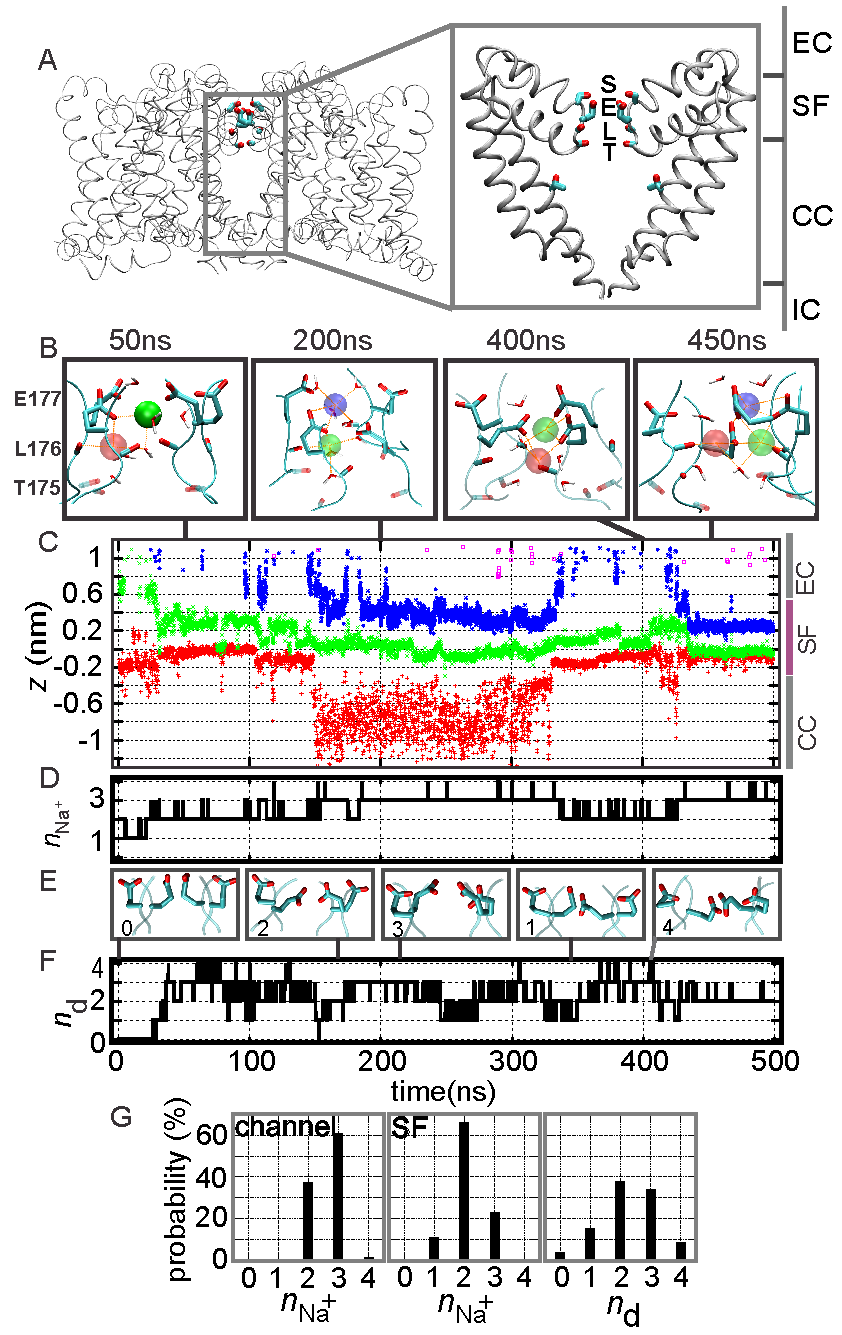
\includegraphics[width=0.5\textwidth]{nav1/Nav1Fig1}
\caption[Sodium movement in the selectivity filter of Na\textsubscript{V}Ab]{\textbf{Sodium movement in the selectivity filter of Na\textsubscript{V}Ab}. (\textbf{A}) Crystallographic structure of Na\textsubscript{V}Ab with a close up of the central ion permeation pore in which the helices above and below the plane of the page have been omitted for clarity.  The constriction of the pore is formed by loops lined with the T175,L176,E177,S178 sequence (the selectivity filter).  The only hydrophilic residue in the central cavity (CC), T206, is also shown.  The IC gate is occluded. (\textbf{B}) Representative snapshots of sodium ions (spheres) in the SF are shown at specified time steps.  The backbone carbonyl groups of T175 and L176 and the side chains of E177 are shown, together with the water molecules involved in the coordination (yellow lines) of permeating ions. (\textbf{C}) Movement of Na$^+$ ions along the pore axis.  By convention, the ions are colored red, green, blue, and purple from the innermost to the outermost position in the channel.  Spontaneous and reversible diffusion of Na$^+$ ions along the channel axis occurred, with visible knock-on and knock-off events at t = 145 and 330 ns, respectively, as the blue and red ions displace each other out of the SF (z = 0 corresponds to the mean axial position of the carbonyl C atom of L176). (\textbf{D}) Time evolution of the number of Na$^+$ ions in the pore. (\textbf{E}) The five conformational states of the EEEE ring, with E177 side-chains pointing either out towards the EC mouth or into the SF lumen (ions not shown). (\textbf{F}) Time evolution of the number of E177 side-chains pointing into the SF. (\textbf{G}) Distribution of ionic populations, and E177 side-chain dunking, from 17 $\mu$s of combined MD trajectories.  Ionic occupancy is shown successively for the entire pore, from the EC funnel to the end of the CC (-0.8 nm $\leq$ z $\leq$ 1.6 nm) and for the SF (-0.53 nm $\leq$ z $\leq$ 0.3 nm).  The pore contains 2, 3 or 4 Na$^+$ ions $36\pm4\%$, $63\pm4\%$, and $2\pm1\%$ of the time, respectively (first panel).  The probabilities of finding 1, 2, or 3 ions in the SF are $11\pm2\%$, $66\pm3\%$, and $23\pm3\%$, respectively (second panel). The probabilities of finding 0, 1, 2, 3 or 4 E177 side-chains in dunked conformations are $4\pm1\%$,$16\pm2\%$, $38\pm3\%$, and $8\pm2\%$, respectively (third panel).}
\label{fig:nav1fig1}
\end{figure}

In the Na\textsubscript{V}Ab structure (Fig. \ref{fig:nav1fig1} A), permeating ions move first into an open extracellular (EC) vestibule, through the narrow SF lined by S178, E177, L176, and T175, and into a central cavity (CC) before exiting through the activation gate.  Although the activation gate at the IC end of the channel is closed, Na$^+$ ions spontaneously traveled in and out of the pore during the course of the simulations (Fig. \ref{fig:nav1fig1} B, C).  The movement of Na$^+$ along the pore axis is shown in two representative 500-ns trajectories and Na$^+$ binding modes (Fig. \ref{fig:nav1fig1} B, C; Fig. \ref{fig:nav1figS2} A,B).  When bound to the channel, Na$^+$ ions were at least partly solvated by one or more carboxylate groups of E177 (Fig. \ref{fig:nav1fig1} B; Fig. \ref{fig:nav1figS2} A).  Using this criterion to define the SF leads to approximate axial SF boundaries of -0.53  z  0.3 nm, where z=0 at the L176 carbonyl.  
In the example depicted in Fig. \ref{fig:nav1fig1}, the first ion (red) permeated through the SF and into the CC, and remained trapped in the pore, occasionally returning to the SF.  A second (green) ion entered the SF at t $\approx$ 21 ns and remained there for the rest of the simulation.  Ionic replacement in the SF occurred at t $\sim$ 150 ns, when the entry of a third (blue) ion forced the expulsion of the red ion to the CC, where it rapidly ``bounced'' up and down as it was no longer directly coordinated to the channel.  This ``knock on'' event was followed by a reverse ``knock off'' process at t $\approx$ 332 ns, when reentry of the red ion into the SF expelled the blue ion to the EC.  Subsequent reentry of a blue ion at t $\approx$ 426 ns did not lead to the expulsion of the red ion from the SF; instead, all three ions resided in the SF for the rest of the trajectory (Fig. \ref{fig:nav1fig1} D).  Na$^+$ movements are accompanied by movements of the side chains of E177 residues, which change their conformation from an outward orientation to an inward ``dunked'' orientation (Fig. \ref{fig:nav1fig1} E-F). 

Although the pore was initially devoid of Na$^+$, two ions penetrated into the channel sequentially within 40 ns in all 47 trajectories.  Based on the time trajectories for a combined 17 $\mu s$ of simulation time, the number of sodium ions present in the pore following this initial equilibration period fluctuated between 2, 3, and 4, respectively 36$\pm$4\%, 63$\pm$4\%, and 2$\pm$1\%  of the time; in the SF, double occupancy (66$\pm$3\%) prevailed over single ($11\pm2\%$) and triple (23$\pm$3\%) occupancy (Fig. \ref{fig:nav1fig1} G).  The average SF occupancy was 2.09 $\pm$ 0.05. Note that the statistical uncertainties reported in this work are the standard error of the mean.

\begin{figure}[!ptb]
\centering
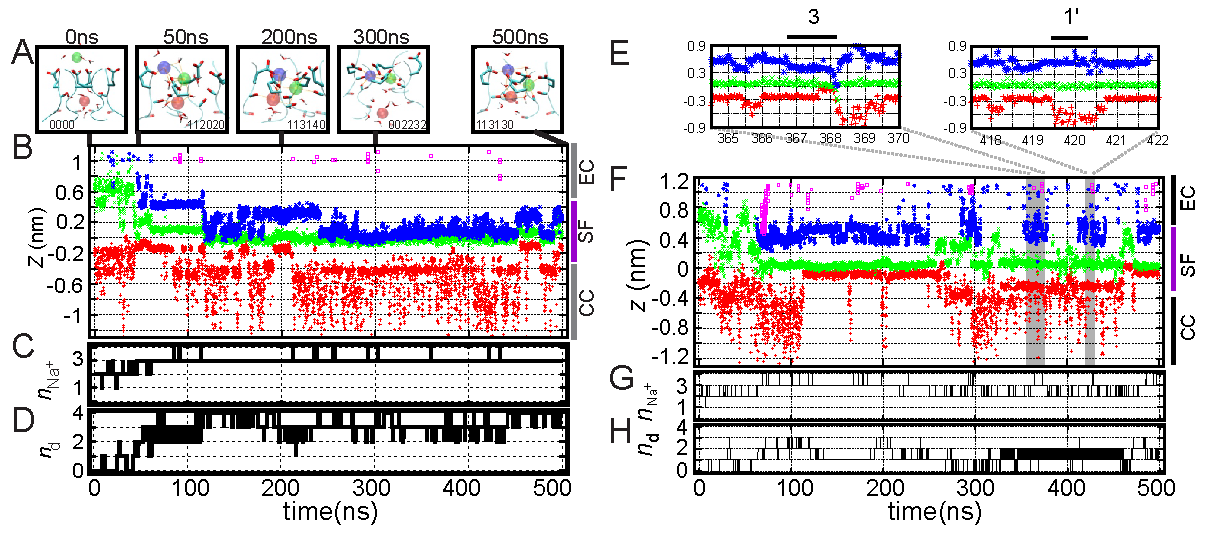
\includegraphics[width=0.9\textwidth]{nav1/Nav1FigS2}
\caption[Two example 500-ns MD trajectories illustrating the dynamics of Na$^+$ ions in the channel lumen]{\textbf{Two example 500-ns MD trajectories illustrating the dynamics of Na$^+$ ions in the channel lumen}. (\textbf{A}) Snapshots of permeating sodium ions, their coordination pattern and the selectivity filter are shown at time steps mentioned.  (\textbf{B,F}) Time evolution of the position of Na$^+$ along the channel axis.  Sodium ions are colored according to their position along channel axis: red, green, blue, and purple, from the innermost to the outermost position, respectively.  In this trajectory, the blue ion remains in the SF following early entry from the EC medium.  (\textbf{C,G}) Number of Na$^+$ ions in the pore. (\textbf{D,H}) Number of E177 side-chains protruding into the lumen (``dunked''). (\textbf{E}) 3-ion and 1- ion intermediate coordination states are highlighted at t = 367-368 ns and t = 420 ns, respectively. }
\label{fig:nav1figS2}
\end{figure}

\subsection{Solvation, Binding, and Energetics of Na$^+$ in the Selectivity Filter}
The movement of Na$^+$ in and out of the pore involves changes in the ionic occupancy of the SF.  To uncover the relationship between ionic binding and mobility, we first decompose the axial distribution of Na$^+$ according to coordination by water and channel groups (Fig. \ref{fig:nav1fig2}).  The axial distribution of channel O atoms in the lumen of the pore is shown in Fig.  \ref{fig:nav1fig2} A.  When in the SF region, Na$^+$ is bound to carboxylate O atoms of E177 only (Fig. \ref{fig:nav1fig2} B, green) or to carboxylates of E177 and carbonyls of L176 together (Fig. \ref{fig:nav1fig2} B, yellow).  Accordingly, we define binding to the SF by carboxylate coordination of Na$^+$.  The bimodal distribution of Na$^+$ in the SF peaks at z = -0.3 and 0 nm, which nearly matches the average positions of E177 carboxyl and L176 carbonyl O atoms, corresponds to two distinct binding modes (E-only and E-, L-bound, respectively). 

\begin{figure}[!htb]
\centering
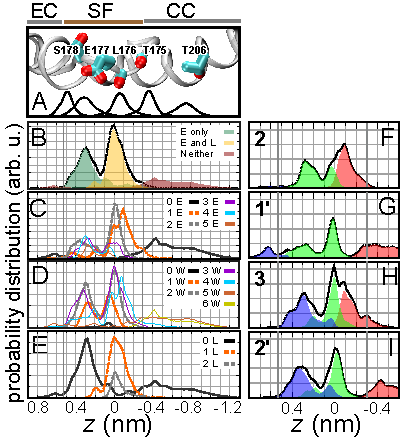
\includegraphics[width=0.5\textwidth]{nav1/Nav1Fig2}
\caption[Sodium binding and occupancy]{\textbf{Sodium binding and occupancy}. (\textbf{A}) Axial distribution of channel O atoms involved in the solvation of permeating Na$^+$ ions, from the hydroxyl groups of S178 and T206, the carboxyl group of E177, and the carbonyl groups of L176 and T175. (\textbf{B}) Axial distribution of Na$^+$ atoms in the SF and CC regions of the channel, distinguishing between states in which Na$^+$ is directly bound to E177 (``E'', green), to both E177 and L176 (``EL'', yellow), or to neither (brown).  The SF is defined by two spatially resolved Na$^+$ binding sites, E and EL.  The small peaks at z = -0.65 and z = 0.40 nm in the brown distribution correspond to direct Na$^+$ coordination by the hydroxyl O atom of S178 and water-mediated coordination to the carbonyl O atom of T175, respectively. (\textbf{C-E}) Decomposition of the axial distribution of Na$^+$ ions according to the number of (\textbf{C}) carboxyl O atoms of E177, (\textbf{D}) water molecules, and (\textbf{E}) carbonyl O atoms of L176 present in the first solvation shell of individual Na$^+$ ions. (\textbf{F-I}) Axial distributions of Na$^+$ ions shown successively for ion coordination macrostates 2, 1', 3, and 2', where integers 1 to 3 correspond to the ionic occupancy of the SF and the prime indicates the presence of one Na$^+$ ion in the CC.  Color coding (red, green, blue) is as defined in the legend of Fig. \ref{fig:nav1fig1}.  The total ionic occupancy of the pore is exactly two in states 1' and 2, and exactly three in states 2' and 3.}
\label{fig:nav1fig2}
\end{figure}

The number of carboxyl O atoms in the first solvation of shell of Na$^+$ varies from 1 to 5 throughout the SF, with 2-4 and 1-2 dominating in the E and EL peaks, respectively (Fig. \ref{fig:nav1fig2} C).  Direct coordination by the channel induces partial dehydration of Na$^+$, with the number of water molecules in the first solvation shell of Na$^+$ dropping from 6 or 7 outside of the SF to a range of 1 to 4 in the SF for nearly all ions (Fig. \ref{fig:nav1fig2} D).  In addition, each Na$^+$ is coordinated by one or occasionally two carbonyl O atoms of L176 in the EL binding site (Fig. \ref{fig:nav1fig2} E).  Variations within the SF reflect the presence of multiple, highly-degenerate ionic binding modes, as discussed below.

The analysis of Na$^+$ coordination leads to four distinct macrostates, which we refer to as 1', 2, 2', and 3.  In this notation, the integer refers to the ionic occupancy of the SF, and primed and unprimed states differ in the number of Na$^+$ present in the central cavity, respectively 1 and 0.  The bimodal character of the axial distribution of Na$^+$ in the SF is retained in all four macrostates (Fig. \ref{fig:nav1fig2} F-I).  The relative population of these two peaks depends on the ionic occupancy of the CC, but not on that of the SF.  When no ion is present in the CC, the relative population of E-only and E-, L-bound peaks is approximately 1:2 (35:65 for state 2 and 33:67 for state 3).  In contrast, when one ion is present in the CC, the two binding sites are nearly equivalent, with E:EL-bound ratios of 45:55 and 50:50 in states 1' and 2', respectively.  This moderate shift in Na$^+$ from the EL site to the E site is likely due in part to repulsive coulombic interactions with the cation in the CC.  

To gain insight into the energetics underlying Na$^+$ movement, we computed two-dimensional free energy surfaces for ion pairs in the channel (Fig. \ref{fig:nav1figS4} A,B).  Analysis reveals a relatively small number of well-defined arrangements of ion pairs in the SF, usually comprised of conformations in which adjacent ions are either distributed in the E-only (z = -0.3 nm) and EL (z = 0) sites, and conformations where two ions are in the EL site, with both cases occurring at once in macrostate 3.  The simultaneous presence of two Na$^+$ ions in the EL binding site is made possible by the relative width of the channel and by coordination of the ions by multiple carboxylate groups.  Rearrangements include either concerted (parallel to the diagonal) or sequential (parallel to one axis) movement of Na$^+$ to and from the above two states, with small intervening barriers (<1 kcal/mol).  These features are relatively independent of ionic occupancy (Fig. \ref{fig:nav1figS4}), revealing the surprising ability of the SF to approximately preserve the energy landscape of Na$^+$ ions. Despite these overall similarities, the free energy landscape governing the movement of Na$^+$ between the SF and the CC depends on both the occupancy and the placement of ions in the SF: when two ions are in the pore, the expulsion of the innermost (red) ion from the SF to the CC requires migration of the second (green) ion from the E site to the EL site (Fig. \ref{fig:nav1figS4} C top). When 3 ions are in the pore, the EL site of the SF is usually occupied by the second ion and there is no longer any barrier impeding movement of the innermost Na$^+$ ion between the SF and the CC (Fig. \ref{fig:nav1figS4} C bottom).  These features support a knock-on mechanism involving either 2 or 3 ions, driven at least in part by coulombic repulsion between Na$^+$ ions.  However, in contrast to the single-file, ``Newton balls'' mechanism of K$^+$ permeation in the narrow SF of K$^+$ channels \cite{MoraisCabral:2001bp}, Na$^+$ conductance in Na\textsubscript{V}Ab does not require concerted cation movement, as two Na$^+$ ions can come side-by-side and occasionally pass each other in the relatively wide SF of Na\textsubscript{V}Ab.

\begin{figure}[hp]
\centering
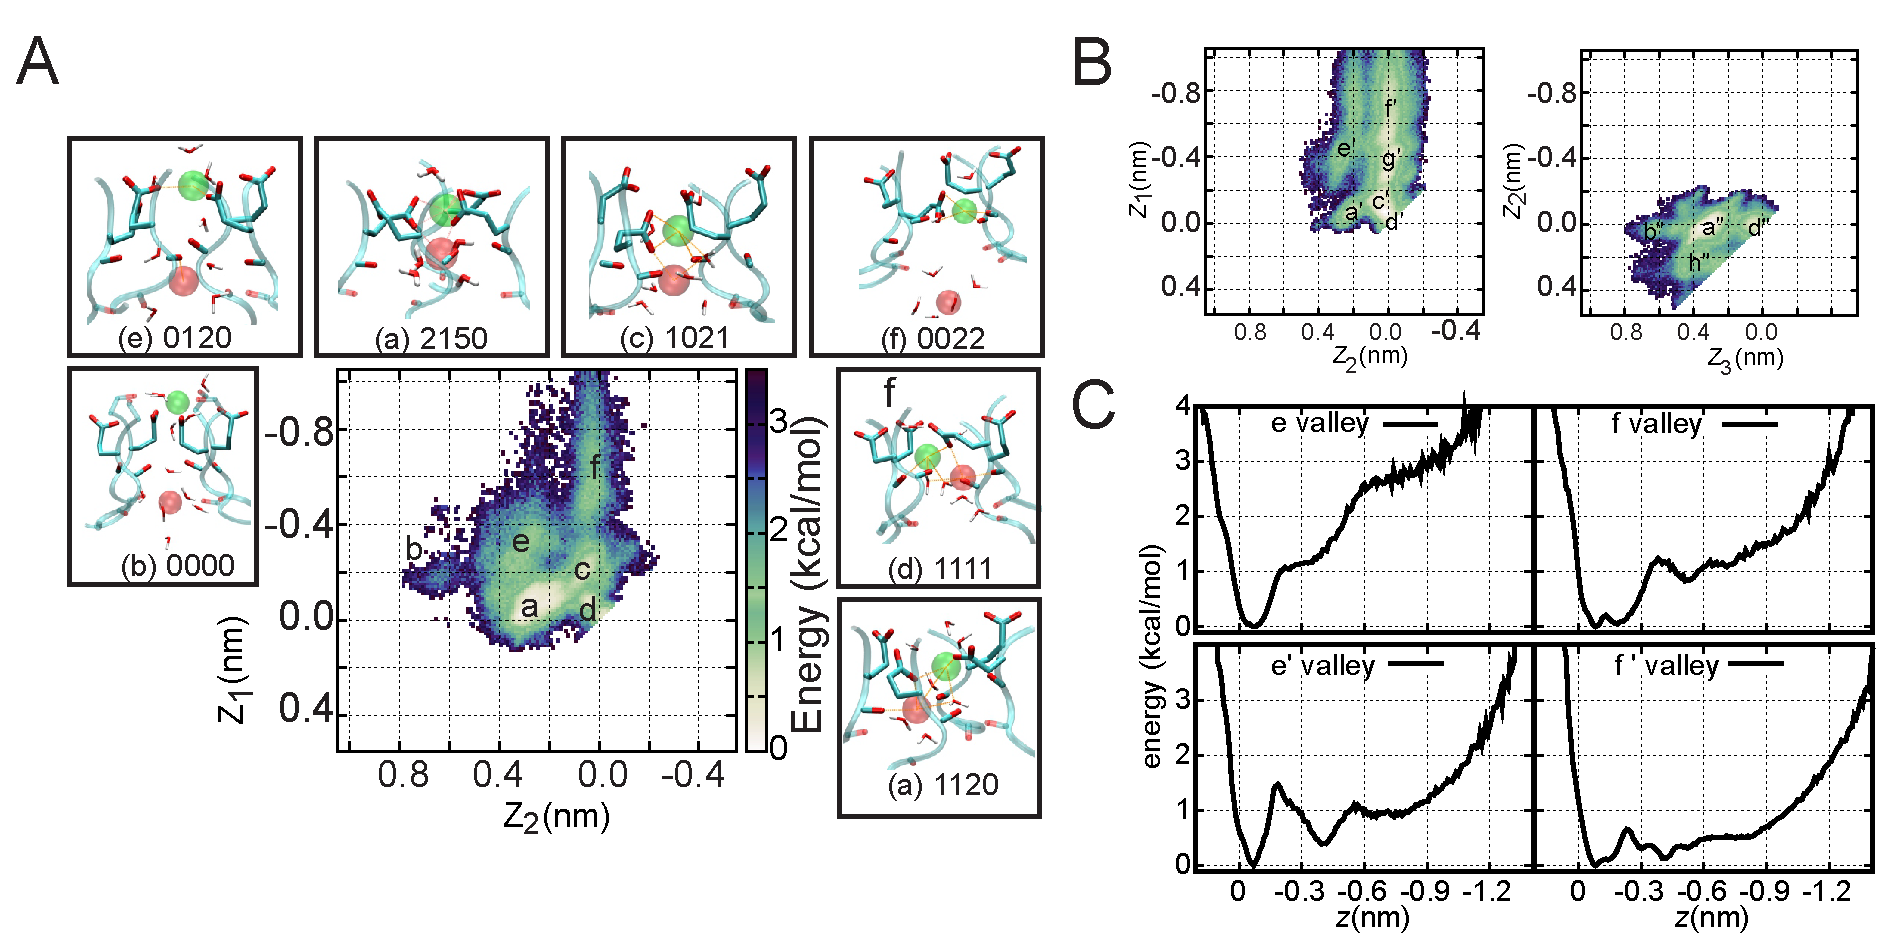
\includegraphics[width=0.9\textwidth]{nav1/Nav1FigS4}
\caption[Free energy landscape of Na$^{+}$ motion in Na\textsubscript{V}Ab]{\textbf{Free energy landscape of Na$^{+}$ motion in Na\textsubscript{V}Ab}. (\textbf{A}) 2D PMF of axial positions of first (red, z$_1$) and second (green, z$_2$) sodium ions in states where two Na$^+$ ions are the channel (macrostates 1' and 2).  The free energy basins are labelled a, c, d, e, and f in order of decreasing occupancy.  Basins a and c are related by concerted ionic motion.  Basin a, the most populated conformation, corresponds to the green and red ions in the E and EL binding modes, respectively (see representative conformations in the insets, where the four-digit code corresponds to E and L coordination).  In basin d, both ions are in the EL-binding mode.   Migration of the green ion from the E binding site (basin e) to the EL binding site (basin f) triggers the expulsion of the red ion into the CC.  (\textbf{B}) 2D PMFs of axial positions of first (red, z$_1$), second (green, z$_2$), and third (blue, z$_3$) sodium ions in triple ionic occupancy macrostates 2' and 3.  (Left) The flat free energy valley defined by d', c', g', and f' suggests that the red ion can diffuse freely between the SF and the CC when the green ion is in the EL binding site (z2 $\approx$ 0).  In basins c' and d', both red and green ions are condensed in the EL binding site.  (Right) Basins b'' to d'' correspond to the stepwise movement of a third (blue) ion in and out of the SF.  Basins a', a'', d', and d'' are equivalent to basins a and d of panel A.  (\textbf{C}) Coupling of ion movement to ionic occupancy of the SF.  Free energy profiles for the movement of the innermost (red) first ion between the selectivity filter (SF) and the central cavity (CC).  The top and bottom panels correspond to total ionic occupancy of two and three Na$^+$ in the channel lumen for (Left) e (top) and e' (bottom) basins; (Right) f and f' basins.  When two ions are in the channel, the expulsion of the innermost ion into the CC is conditional to the presence of a second ion in the EL binding site.  When three ions are in the channel, the presence of the second ion in the EL binding site further facilitates the movement of the innermost ion between the SF and the CC, which becomes diffusive, as suggested by the flat free energy profile in panel f'.}
\label{fig:nav1figS4}
\end{figure}

\subsection{Mechanism and Kinetics of Ion Translocation}

\begin{figure}[!htb]
\centering
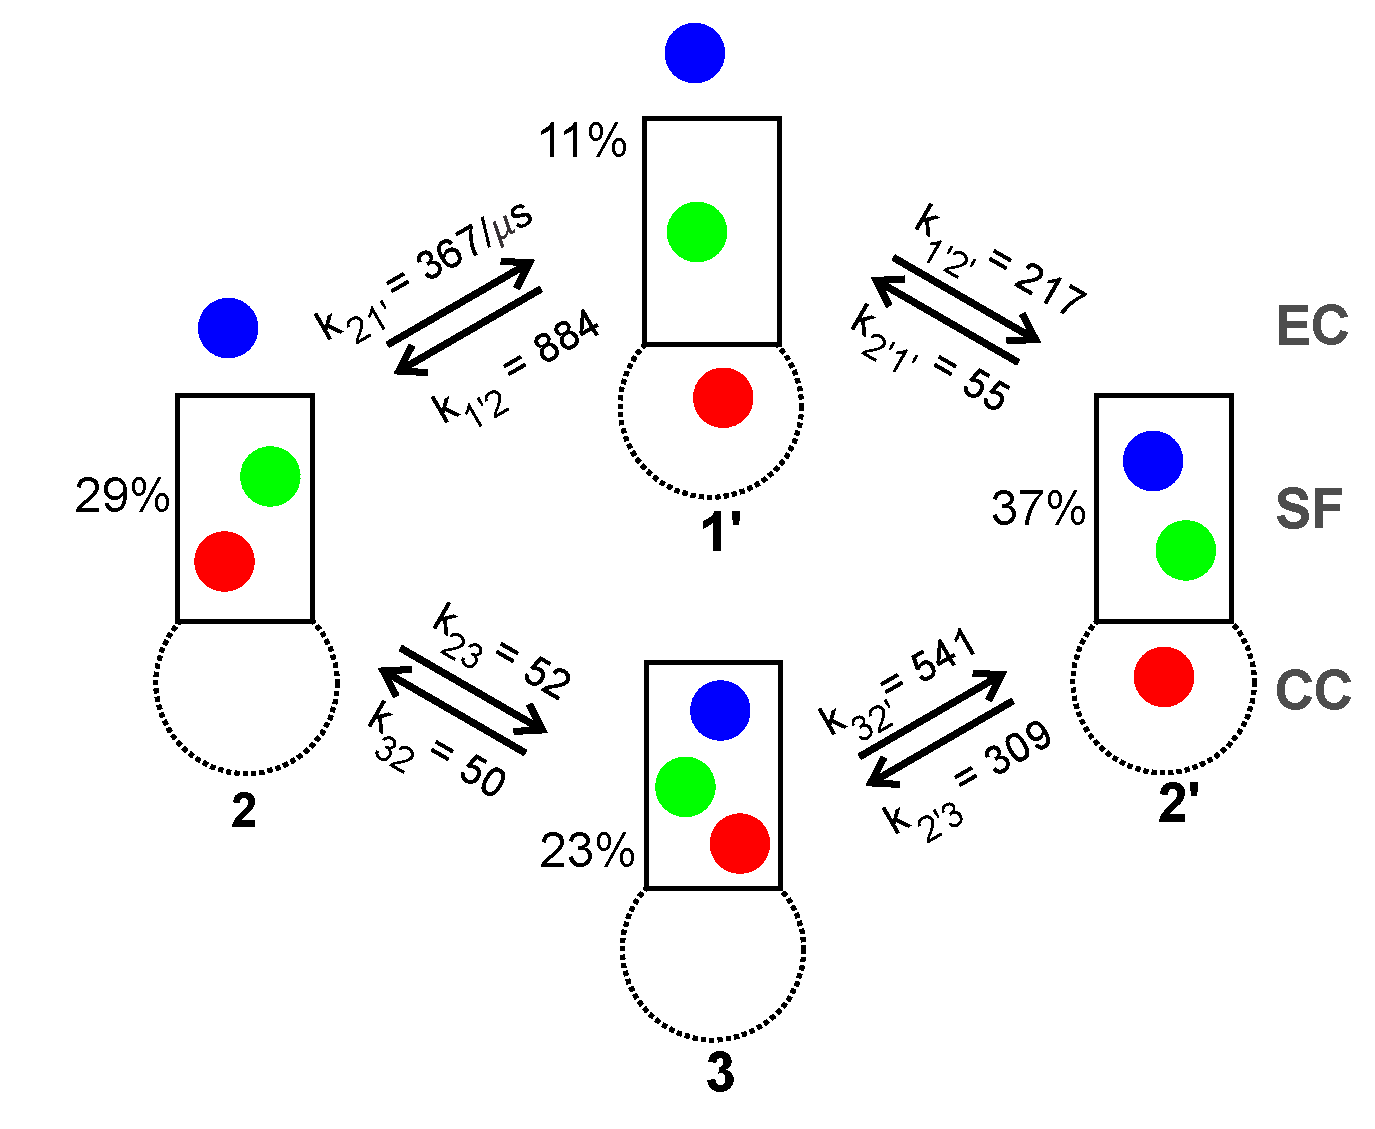
\includegraphics[width=0.9\textwidth]{nav1/Nav1Fig4}
\caption[Mechanism and kinetics of Na$^+$ translocation through the selectivity filter]{\textbf{Mechanism and kinetics of Na$^+$ translocation through the selectivity filter}. The black box represents the SF, with the CC below and the EC mouth above.  Color coding of the ions (spheres) is analogous to that of Figs. \ref{fig:nav1fig1} and \ref{fig:nav1fig2}.  The populations of all four states 1', 2, 2', and 3, which differ in the occupancy of the channel and of the selectivity filter, are shown in \%, and the rate constants computed from the MD trajectories (see Fig. \ref{fig:nav1fig1}) are shown above or below each arrow in units of $\mu s^{-1}$.  At this ionic concentration (150 mM), states 2 and 2' correspond to the resting state of the system. The exchange between states 2 and 2', which corresponds to a unitary ionic translocation through the selectivity filter, involves either one-ion or three-ion intermediate states.}
\label{fig:nav1fig3}
\end{figure}

The analysis of transitions between macrostates 1', 2, 2', and 3 leads to the mechanism depicted in Fig. \ref{fig:nav1fig3} A.  Since two-thirds of all conformations correspond to states 2 and 2', we consider that the resting state of the SF holds two ions, at least in the present, ``pre-open'' state of the channel.  Although a small number of apparently concerted transitions between states 2 and 2' occurred within the time resolution of this analysis (25 ps), most transitions occurred sequentially, either via one-ion or three-ion intermediate states 1' and 3, respectively, depending on whether entry into the SF preceded exit from the SF, or the other way round (a time series illustrating both of these pathways is shown in Fig. \ref{fig:nav1figS2} E-H).  The rates of these transitions are comparable for the two pathways, with the path via the one-ion intermediate being slightly faster.  The mean first passage times for 2$\rightarrow$1'$\rightarrow$2' and 2$\rightarrow$3$\rightarrow$2' translocation events (irrespective of direction) are 0.96 and 6.8 ns, respectively.   

Nearly equal numbers of forward and reverse transitions between the four macrostates depicted were achieved over the set of simulations.  A total of 201 spontaneous Na$^+$ translocation events through the SF occurred within 17 $\mu s$ of simulation, 112 and 75 of which travelled through states 1' and 3, respectively, and 14 of which were direct exchanges.  These ionic permeation events yield an estimated rate of ion flow of $(6 \pm 1 \mu s^{-1}$ through the SF, which is in the range of typical single ion channel permeation rates of 1 to 10 $\mu s^{-1}$ \cite{Hille:2001tw}.  Although the IC gate is closed, this result suggests that the SF is in its functional state and that the rates would not change appreciably if the IC channel gate were open.  The fact that the CC is occupied 48\% of the time indicates that the chemical potential of Na$^+$ in the CC is essentially identical to that in the EC solution at this concentration.  Therefore, the observed diffusion of Na$^+$ through the SF is relevant to Na$^+$ movement in the open state of the channel at 0 mV under conditions of equilibrium (i.e., in the absence of an electrochemical gradient).  

Despite the high mobility of Na$^+$ in the CC (Fig. \ref{fig:nav1fig1} C, Fig. \ref{fig:nav1figS2}), our results suggest that the CC is a binding site for Na$^+$.  The energetics of Na$^+$ binding in the CC and the SF are coupled: there is always one Na$^+$ ion in the CC when a single ion is in the SF (state 1') and triple ionic occupancy of the SF occurs only when the CC is empty (state 3).  However, whether or not the CC is part of the Na$^+$ conduction mechanism may depend on Na$^+$ occupancy at physiological conditions.  Due to the much lower concentration of free Na$^+$ in the cytoplasm (5 mM in humans, 8 mM in \textit{E. coli} \cite{Maguire:2002wu}) than in our simulations (150 mM), the presence of a physiological electrochemical gradient across the membrane is likely to lead to a decreased Na$^+$ occupancy of the CC in the open state of the channel, which could drop by a factor of up to 150/5 = 30.  In that limit, Na$^+$ permeation may occur primarily via alternating macrostates 2 and 3 (Fig. \ref{fig:nav1fig3}), with a higher average occupancy of the SF. 
Regardless of the actual ionic occupancy of the CC, the present study indicates that the permeation mechanism at high Na$^+$ concentration involves the alternation of states in which a total of 2 Na$^+$ (states 2, 1') and 3 Na$^+$ (states 3, 2') are bound in the pore.  The similar population of overall channel occupancy in states 2 and 3 suggests that their exchange underpins an effective knock-on/knock-off process.  Transitions involving the exchange of Na$^+$ between the EC vestibule and the SF are the slowest observed between the four macrostates in Fig. \ref{fig:nav1fig3}, of the order of 50 $\mu s^{-1}$, indicating that the rate-limiting step for the translocation of Na$^+$ through the SF is the migration of the 3rd (blue) ion between the EC and the SF.  By contrast, the movement of Na$^+$ between the SF and the CC is faster by an order of magnitude, a feature that is likely to persist upon directional movement from the SF to the CC in the open state of the channel.

\subsection{Coupling of Channel Structure and Dynamics to Na$^+$ Permeation}

\begin{figure}[!htb]
\centering
\includegraphics[width=0.9\textwidth]{nav1/Nav1FigS8}
\caption[Coupling of channel structure and dynamics to Na+ solvation and mobility]{\textbf{Coupling of channel structure and dynamics to Na+ solvation and mobility}. (\textbf{A}) 2D PMFs of $\chi_{1}$(C$_{\alpha}$-C$_{\beta}$) vs. $\chi_{2}$(C$_{\beta}$-C$_{\gamma}$) for E177 residues successively in the presence (left) and in the absence (right) of excess NaCl salt.  Out-facing and lumen-facing (``dunked'') conformations of E177 are characterized by g$^{+}$ and g$^{-}$ $\chi_{2}$ conformations, respectively.  The presence of Na$^+$ displaces the conformational equilibrium of individual E177 side-chains towards the dunked state. (\textbf{B}) Representative conformations of E177 and S178 side-chains (left) with and (right) without 150-mM NaCl salt; (top) side and (bottom) EC views of the SF.  Conformational dunking allows direct coordination of Na$^+$ ions (left).  In the out-facing conformation, E177 sidechains make hydrogen bonds with the hydroxyl groups of S178 (right). (\textbf{C}) Time evolution of the survival probability of the $\chi_{2}$ dihedral angle of E177 in dunked (``Dunk'') and undunked (``Undunk'') states, shown with a fit to a multiple exponential function.  The fits to the survival probability of the dunked and undunked states in the presence of 150mM NaCl are S(t) = 0.56 exp(-t/0.049)+0.27 exp(-t/0.667)+0.14 exp(-t/8.180) and S(t)=0.51 exp(-t/0.068)+0.29 exp(-t/0.788)+0.16 exp(-t/9.047), respectively, with time t expressed in ns.  In the absence of salt, the exponential fits for dunked and undunked states are S(t) = 0.70 exp(-t/0.012)+0.11 exp(-t/0.09) and S(t)=0.77 exp(-t/0.012)+0.16 exp(-t/0.325)+0.05 exp(-t/8.044), respectively.  Correlation coefficients for these fits were 0.997 or better. (\textbf{D}) Time evolution of the axial projection of centers of cationic charge (CCC) and of anionic charge (CAC) within the channel lumen.  (Black) Average axial position of Na+ ions located inside the SF (0.6$\leq$z$\leq$-0.24 nm, delineated by thick grey lines); (orange) average axial position of carboxylate oxygen atoms of E177 side chains.  Initially, (t$\leq$100 ns), the motions of the CAC and the CCC are uncorrelated (Pearson correlation coefficient p=-0.12), whereas in 100-300 ns and 300-500 ns time segments they show significant correlation (p=0.72 and 0.75).  Based on this analysis, we identify a tight-coupling region (TCR) within which cationic movement is coupled to the movement of E177 side chains.}
\label{fig:nav1figS8}
\end{figure}

Na$^+$ coordination induced rapid and reversible conformational isomerization or ``dunking'' of E177 side chains, bringing their carboxylate group from out-facing to protruding into the lumen (Fig. \ref{fig:nav1fig1} E, F).  Coordination of Na$^+$ by E177 occurred mostly in the dunked conformation, which was much more likely in the presence than in the absence of cations, with the equilibrium constant to dunked vs out-facing conformations of E177 increasing from K$_{dunk}$ = 0.04 $\pm$ 0.02 to 1.7 $\pm$ 0.2 upon addition of salt (Fig. \ref{fig:nav1figS8} A, B).  Moreover, conformational isomerization of E177 occurred on the same time scale as Na$^+$ movement.  Multiple exponential fitting of the survival probabilities of Glu side-chain conformations yields three conformational relaxation times in the order of 0.1, 1, and 10 ns, respectively (Fig. \ref{fig:nav1figS8} A).  The two longer relaxation times are commensurate with the mean first-passage-times of Na$^+$ exchange through the SF, and the longest relaxation time of the dunked state disappears in the absence of salt.  Accordingly, the axial displacement of the center of charge of the carboxylate groups is statistically correlated (Pearson coefficient > 0.7) to that of Na$^+$ ions within the center of the SF region (Fig. \ref{fig:nav1figS8} B).

To uncover the mechanism coupling channel conformational dynamics to ion binding and mobility, we examined the coordination of Na$^+$ by channel O atoms throughout the simulations.  Each microstate (snapshot) was assigned a 6-digit code describing the number of E177 carboxylate and L176 carbonyl O atoms in the first solvation shell of red, green, and blue ions, defining a SF binding mode.  A myriad of distinct ionic coordination states were observed.  A network representation combining the most likely binding modes observed in the entire simulation data set is shown in Fig. \ref{fig:nav1fig5} together with representative snapshots.  Each of these binding modes belongs to one of microstates 1', 2, 2', or 3 and is represented by a node whose area is proportional to its relative population; transitions observed between any two nodes are represented by an edge whose thickness is proportional to flux.  The nodes in the network are highly connected.  This analysis reveals the staggering multiplicity and degeneracy of ionic arrangements combining Na$^+$ ions and COO- groups, whose complementary charges enable their condensation into clusters - particularly in the EL binding site, which often accommodates multiple Na$^+$ ions in close proximity.  In these ionic clusters, Na$^+$ ions are often bound to more than one Glu side chain, and vice versa.  Many individual transitions involve unitary changes in carboxylate O coordination and occur within ~100 ps, the faster timescale of Glu conformational relaxation.  These changes result in the rapid interconversion of ionic arrangements in a fashion reminiscent of a highly-disordered, liquid-like state. 

\begin{figure}[hp]
\centering
\includegraphics[width=0.9\textwidth]{nav1/Nav1FigS7}
\caption[Network representation highlighting the multiplicity and degeneracy of Na$^+$ binding modes]{\textbf{Network representation highlighting the multiplicity and degeneracy of Na$^+$ binding modes}. Each of the four macrostates (1', 2, 2', and 3) corresponds to a large number of microstates (Na$^+$ binding modes) differing in the number of carboxylate O atoms of E177 and carbonyl O atoms of L176 directly coordinating Na$^+$ ions.  Out of a total of 1,233 microstates observed, the 521 most populated binding modes, which account for 99\% of the total population, are depicted as disks whose surface area is proportional to their population.  Each line connecting two states, an edge, represents transitions between these states, with edge thickness proportional to the number of transitions.  The network is clustered and colored using a modularity algorithm which contains no information about the four macrostates, only edge connectivity.  A representative snapshot and the distribution of the number of dunked E177 side-chains are shown as insets for each macrostate.}
\label{fig:nav1fig5}
\end{figure}

More often than not, the ionic clusters are not neutral.  Although there is an overall correlation, there is no simple correspondence between ionic occupancy states and the number of dunked side chains, n$_d$, which fluctuated within all the macrostates (Fig. \ref{fig:nav1fig1} F; Fig. \ref{fig:nav1fig5} insets) and even between closely related microstates.  Charge fluctuations in the ionic cluster result from the impossibility of maximizing attractive interactions between opposite charges while simultaneously minimizing repulsion between like charges and satisfying the spatial constraints imposed by the architecture of the SF.  Together, these factors contribute to the multiplicity and degeneracy of ionic binding modes.  In turn, the fluidity of ionic coordination underpins the high mobility of Na$^+$ in the SF.  By guaranteeing that no single binding mode is significantly stabilized over any other one and that the barriers separating them are low, the conformational flexibility of the EEEE ring shapes an energy landscape conducive to ionic diffusion in the SF and, ultimately, to Na$^+$ permeation. 

\subsection{A Multi-state Knock-on Mechanism for Na$^+$ Permeation in Na\textsubscript{V}Ab}

Our results reveal spontaneous permeation of Na$^+$ through the selectivity filter of Na\textsubscript{V}Ab in a knock-on mechanism involving alternating states in which 2 or 3 Na$^+$ ions are within the pore lumen.  In contrast to the direct solvation of K$^+$ by backbone carbonyl groups in the narrow SF of K$^+$ channels \cite{Doyle:1998wq,Zhou:2001vo}, binding of Na$^+$ in the shorter and wider SF of Na\textsubscript{V}Ab involves both direct and water-mediated interactions of Na$^+$ with the carbonyl groups of T175 and L176 and with the carboxylate groups of E177.  Furthermore, elementary steps of Na$^+$ diffusion in Na\textsubscript{V}Ab do not occur via linear, concerted movement of an ionic column as in the ``Newton balls'' mechanism of K$^+$ permeation in K$^+$ channels \cite{MoraisCabral:2001bp}, but instead involve liquid-like rearrangements of ionic clusters resulting from the condensation of variable numbers of Na$^+$ ions and carboxylate groups.  Evidently, as early in evolution as bacteria, two fundamentally different structures and mechanisms had arisen for conduction of Na$^+$ versus K$^+$ in ion channels.  

In contrast to the classic ``snug'' or ``induced fit'' models of ion permeation, it is becoming recognized that protein flexibility plays a role in selective ion transport \cite{Roux:2011ed,Andersen:2011ty}.  The mechanism uncovered in the present study highlights the interplay of channel dynamics and ion movement.  In the ionic clusters of Na$^+$ and E177 carboxylates in the SF of Na\textsubscript{V}Ab, negative and positive charges are nearly but not exactly compensated.  Far from trapping ions, the reciprocal coordination of permeating Na$^+$ ions and carboxylate groups creates a myriad of ionic binding modes and a highly-degenerate energy landscape propitious to the rapid exchange and diffusion of ions through the SF.  Dynamic coupling of ionic coordination to conformational isomerization of the E177 side chains guarantees at once the multivalency of the SF for Na$^+$ ions and the rapid exchange between alternating states differing in the number of bound ions, resulting in an effective knock-on rate of $6\times10^{6}$ $s^{-1}$.  This unique catalytic mechanism takes advantage of the degeneracy of ionic interactions to accelerate Na$^+$ movement toward the limit of free diffusion.  In upcoming studies, we will examine how this catalytic mechanism is affected by the replacement of Na$^+$ by the other primary physiological cations, K$^+$ and Ca$^2+$, and by the replacement of Glu by the shorter Asp side chain.

In eukaryotes, voltage-gated Na$^+$ channels are composed of four covalently-linked domains similar to one subunit of Na\textsubscript{V}Ab \cite{Hille:2001tw,Catterall:2000vb,Catterall:2012fh,Bezanilla:2008ht}. This arrangement places the amino acid residues DEKA in the positions of EEEE in homotetrameric Na\textsubscript{V}Ab \cite{Heinemann:1992ep}. The mechanism of Na$^+$ permeation described here would be substantially different if DEKA were present at the positions of the four E177 residues in Na\textsubscript{V}Ab.  Further structural and computational studies will be required to understand the mechanistic significance of this profound difference in structure of the SF of bacterial and eukaryotic Na$^+$ channels. 

\section{Methods} 
The simulation system consisted of the Na\textsubscript{V}Ab I217C mutant based on the crystallographic structure with the highest resolution (PDB code: 3RVY) \cite{Payandeh:2012ib}, embedded in a hydrated 1,2-dimyristoyl-sn-glycero-3-phosphatidylcholine (DMPC) bilayer, yielding a system comprising ~219,000 atoms.  The simulations were performed with GROMACS 4.0.7 \cite{Hess:2008db}.  The protein and ions were modeled with the OPLS all-atom force field \cite{Jorgensen:1996vx,Kaminski:2001eq}, and the TIP3P model \cite{Jorgensen:1983ty} was used for water molecules.  The lipid bilayer was modeled by the Berger parameters \cite{Berger:1997bc} using the half-$\epsilon$ double-pairlist method \cite{Chakrabarti:2010gf}.  Forty-seven unconstrained simulations of 400-to-500-ns each yielded 23 $\mu s$ of simulation data.  To check the dependency of our results on the force field, we generated a 340-ns-long simulation with the CHARMM force field \cite{MacKerell:1998tp}. Although this control simulation is too short for a quantitative comparison, results confirm multiple Na$^+$ occupancy in two binding sites involving direct coordination to E177 and L176, as well as conformational isomerization of the Glu side chain and formation of ionic clusters, consistent with the mechanism described above.

\printbibliography[heading=subbibnumbered,title={References}]
 \end{refsection}
 \begin{refsection}
 \chapter{Simulation Studies of Ion Permeation and Selectivity in Nav Channels}
 
The contents of this section were adapted from an article published in the \textit{Current Topics in Membranes} and reproduced here with permission.\par
\bigskip
Reference: Ing, C., \& Pom\`es, R. (2016). Simulation Studies of Ion Permeation and Selectivity in Voltage-Gated Sodium Channels. In \textit{Current Topics in Membranes} (Vol. 78, pp. 215-260). Elsevier.\par
\bigskip
Contributions: The manuscript was written and edited by C.I. and R.P.

\newpage
 
 \section{Summary}
 
 Voltage-gated ion channels are responsible for the generation and propagation of action potentials in electrically excitable cells.  Molecular dynamics simulations have become a useful tool to study the molecular basis of ion transport in atomistic models of voltage-gated ion channels.  The elucidation of several three-dimensional structures of bacterial voltage-gated sodium channels (Nav) in 2011 and 2012 opened the way to make detailed computational investigations of this important class of membrane proteins.  Here we review the numerous simulation studies of Na$^{+}$ permeation and selectivity in bacterial Nav channels published in the past five years.  These studies use a variety of simulation methodologies differing in force field parameters, molecular models, sampling algorithms, and simulation times.  Although results disagree on the details of ion permeation mechanisms, they concur in the presence of two primary Na$^{+}$ binding sites in the selectivity filter and support a loosely-coupled knock-on mechanism of Na$^{+}$ permeation.  Comparative studies of Na$^{+}$, K$^{+}$, and Ca$^{2+}$ permeation reveal sites within Nav channels that are Na$^{+}$ selective, yet a consensus model of selectivity has not been established.  We discuss the agreement between simulation and experimental results, and propose strategies that may be used to resolve discrepancies between simulation studies in order to improve future computational studies of permeation and selectivity in ion channels.
 
 \section{Introduction}
 
 In both eukaryotic and prokaryotic organisms, ion channels are a class of transmembrane proteins that facilitate critical physiological processes such as nerve impulses, muscle contraction, and cell signaling \cite{Hille:2001tw,Zheng:2015vj}. In excitable cells, two types of voltage-gated ion channels called Nav and Kv channels that specialize in Na$^{+}$ and K$^{+}$ permeation, respectively, open and close in response to transmembrane voltage and allow for one or the other of these cations to flow according to its electrochemical gradient.  In mammalian skeletal muscle, the extracellular ion concentrations of Na$^{+}$ and K$^{+}$ are 145 mM and 4 mM, while intracellular ion concentrations are 12 mM and 155 mM, respectively \cite{Ashcroft:2000ts,Hille:2001tw}.  This concentration asymmetry is exploited in a process involving selective ion permeation, with Na$^{+}$ influx through Nav channels and K$^{+}$ efflux through Kv channels giving rise to the rising and decay phases of an action potential, respectively. To understand the function of wildtype ion channels as well as disease-causing mutations \cite{Ashcroft:2000ts,Hille:2001tw}, it is essential to elucidate the molecular basis for selective ion permeation.
The aim of this review is to present a critical analysis and discussion of the major findings of the computational studies published to date on ion permeation and selectivity in voltage-gated Nav channels.  First, we present an overview of published computational studies of sodium channels, discussing methodological considerations such as force field, channel model, and sampling technique (Section 1).  We systematically review the Na$^{+}$ binding sites and permeation mechanisms observed in simulation studies of Nav channels (Section 2).  We then review computational studies of the selectivity of Nav channel for Na$^{+}$ over K$^{+}$, as well as Na$^{+}$ over Ca$^{2+}$ (Section 3).  Finally, we discuss the agreement and disagreement of these research findings (Section 4) and make recommendations for future computational studies of voltage-gated sodium channels (Section 5).
 
 \section{Molecular Simulations of Sodium Channels}
 
 Computer simulations of ion channels may be used to identify the molecular driving forces for ion binding, permeation, and selectivity.  In order to study these concepts, a simulation methodology must be selected that establishes a channel model, a force field, a sampling algorithm, and the extent of sampling.  The accuracy of simulation results depends heavily on these methodological choices due to a combination of both systematic and statistical errors.  Statistical errors refer to limitations due to insufficient data set sizes, whereas systematic errors reflect biases resulting not only from inherent limitations of the force field and of the channel model, as well as from the simulation protocol itself.  Sampling errors include both statistical and systematic errors.  Systematic sampling errors arise from imperfect initial conditions, which incur a need for equilibration of the system, and from rare conformational transitions due to ``hidden'' or unforeseen energy barriers, which can make equilibration exceed the time of the simulations (Neale et al. 2013).  Before discussing simulation results, in this section we provide an overview of the methods utilized in computational studies of Nav channels (see Table \ref{table:biased},\ref{table:unbiased}) and comment briefly on their relationship to simulation error.
 
 \subsection{Channel Model and Force Field}
 Known structures of sodium channels differ not only in the amino acid sequence of the pore domain, but also in the presence of voltage-sensing or intracellular domains and in the openness of the intracellular gate (as discussed in Section 2).  The latter two elements may contribute to systematic simulation errors that cannot be reduced by long simulation timescales.  Most studies of ion permeation and selectivity were conducted in a closed NavAb channel under the assumption that the state of the intracellular gate is decoupled from the selectivity filter. This assumption is supported by the high degree of structural similarity of the SF in open and closed channel structures \cite{Payandeh:2012ib,Bagneris:2014eh} and that permeation and selectivity are therefore unaffected.  In simulations conducted in the open NavMs channel, strong structural restraints on transmembrane helices were needed in order to prevent the closure of the intracellular gate.  Although the NavMs channel is functional without voltage-sensing domains, the effect of structural restraints on the structure and dynamic fluctuations of the pore domain has not been quantified and presents a possible source of systematic force field error.  Simulations utilizing structural restraints during production simulations are noted in Tables \ref{table:biased}-\ref{table:unbiased}. 
An accurate model to study ion conduction and selectivity is one in which the channel samples conformations as close as possible to the physiological or experimental environment.  Most ion channel models obtained from crystallographic structures are inherently out of equilibrium due to the crystal packing, which may not be representative of the native environment of the lipid bilayer, and underdetermined side chain orientations due to limited structural resolution.  As such, these models must be allowed to equilibrate at physiological temperature, pressure, and ion concentration in a lipid bilayer in order to adopt a conformation that is less biased by these factors \cite{Kandt:2007wz}.  All simulations were performed at physiological temperature (300-320 K) and pressure (1 atm), but higher than physiological ion concentrations were often used (300-500 mM).  A high ion concentration is frequently utilized in unbiased simulations in order to increase sampling of ion binding and permeation events.  The lipid composition of each bilayer varied considerably across studies, including DMPC, DPPC, DOPC, and POPC of various bilayer patch sizes (Table \ref{table:biased},\ref{table:unbiased}). Although the rationale for selecting a lipid species is not strongly justified in any of the studies reviewed herein, it may be selected to reproduce experimental conditions (NavAb was crystallized in a DMPC-based bicelle)\cite{Payandeh:2012ib} to match the size of a hydrophobic belt on the protein-lipid interface of the channel, or because simulations using a specific lipid are frequently performed in the literature. All patch clamp studies of bacterial sodium channels (NavAb, NavMs, and NaChBac) have been performed in mammalian cells, \cite{Payandeh:2012ib, Ulmschneider:2013da, FinolUrdaneta:2014bz} and as such it is extremely challenging to reproduce these complex experimental conditions with molecular models. The indirect effects of the lipid bilayer composition and ionic concentration on the conformational fluctuations of sodium channels is thus an additional source of systematic error.
Simulations of Nav channels have been performed with a number of protein and ion force fields (Table \ref{table:biased}-\ref{table:unbiased}). The majority of these simulations have utilized CHARMM parameters \cite{MacKerell:1998tp,MacKerellJr:2004dv}, with additional studies conducted using OPLS \cite{Jorgensen:1996vx,Kaminski:2001eq} and AMBER parameters \cite{Hornak:2006gx}.  Ions were modeled using parameters of Aqvist \cite{Aqvist:1990ud}, Joung et al. \cite{Joung:2008bp}, Beglov and Roux \cite{Beglov:1994ip}, and Noskov and Roux \cite{Noskov:2008jp}.  Unless otherwise stated, studies are assumed to use the default ion parameters packaged with protein force field.  Some studies using the CHARMM force field included additional non-bonded interaction adjustments for ions and carbonyl oxygen atoms \cite{Noskov:2004tv}.  While force fields are parameterized to reproduce similar experimental and quantum mechanical measurements for folded proteins, they can result in remarkably different results \cite{LindorffLarsen:2012gl,Rauscher:2015jn}.  As such, when comparing simulation studies force fields are a primary source of systematic error that must be carefully considered.
Given that a diverse combination of channel models and force fields have been used to study Nav channels, it is tempting to attribute any possible discrepancies to these factors.  However, to assess the effect of these methodological choices possible, statistical and systematic sampling errors must first be reduced through appropriate sampling.
 
 \subsection{Sampling Technique}
 Various molecular dynamics sampling techniques have been utilized to study ion permeation and selectivity in ion channels.  These techniques can be broadly classified as biased (Table \ref{table:biased}) and unbiased (Table \ref{table:unbiased}) sampling, where bias refers to additional energy terms added on top of the potential energy function or force field.  The accuracy of both of these approaches relies on the convergence of sampling data sets, such that time-averaged measurements can approach true statistical ensemble average measurements in the limit of long sampling times.  In practice, different simulation observables converge on different time scales, requiring careful examination of observables as a function of simulation time.  Such convergence plots, however, are rarely presented in molecular simulation studies of sodium channels.  Sampling is further complicated by long timescale processes inherent in biological systems, whereby the existence of rare (or unanticipated) transitions in ``hidden'' degrees of freedom can impose an unintended bias on conformational sampling even when statistical convergence of an observable appears to have been achieved \cite{Neale:2011jt}.  Here we review both biased and unbiased simulation methodologies used to study sodium channels and describe the advantages and disadvantages of each approach.
 
 \subsubsection{Biased Sampling}
 In biased sampling studies of ion channels, the movement of permeants is forced to follow a pre-defined pathway on a reaction coordinate.  Biased sampling algorithms comprise umbrella sampling \cite{Torrie:1974hs}, metadynamics \cite{Laio:2002ft,Laio:2008iw}, and non-equilibrium pulling approaches based on Jarzynski's equality \cite{Jarzynski:1997uj}.  Standard umbrella sampling methodology in the context of ion channels consists of multiple simulations which include biasing potentials (usually harmonic) on the position of one or more permeating ions.  The outcome of these simulations can be rigorously debiased and assembled a posteriori to produce a potential of mean force (PMF) profile that represents the reversible thermodynamic work or free energy for ion permeation along the pre-defined reaction coordinate.  This reaction coordinate can be mono- or bi-dimensional, leading to 1D- or 2D-PMFs.  In metadynamics, the PMF is determined by introducing a history-dependent potential energy term that biases the motion of ions to escape free energy minima.  Pulling experiments are used to study non-equilibrium processes (such as the movement of ions along an electrochemical gradient) by gradually moving the center of a harmonic biasing force along a reaction coordinate.  The primary advantage of these techniques is that they can efficiently sample the energetics of rare events that may exist along the predefined reaction coordinate.  As such, the effectiveness of biased sampling largely depends on the definition of a reaction coordinate that can capture the physiological conduction mechanism, including but not limited to the number of permeating ions, their relative arrangement, and the range of their motion within the pore.  Umbrella sampling studies typically utilize aggregate sampling of tens to hundreds of nanoseconds to converge the potential energy landscape of ion permeation in ion channels \cite{Allen:2006vy,Fowler:2013bb}.  However, even though biased approaches facilitate sampling along the reaction coordinate, longer time scale simulations may still be required to converge the PMF when other slowly-relaxing degrees of freedom are present.  With this caveat in mind, biased sampling can be used to efficiently compute estimates of ionic binding affinity and free energy barriers, and conduction rates can be approximated from the PMF using transition state theory and stochastic simulations \cite{Berneche:2003ua,Crouzy:1994eg}.
 
 \subsubsection{Unbiased Sampling}
 In unbiased sampling approaches, the movement of ions is not restrained and simulations can be performed either at equilibrium or in non-equilibrium conditions (such as in the presence of an ionic gradient or an external applied voltage).  In this approach, ions diffuse in and out of the channel as governed by the force field and molecular dynamics algorithm.  The main advantage of this approach is that ion conduction can proceed without requiring assumptions about a reaction coordinate (such as ionic degrees of freedom or ionic occupancy of the pore).  Consequently, conformational states and transitions can be observed that may have otherwise been precluded or discouraged in biased simulations as a result of a suboptimal choice of reaction coordinate.  Variable ionic occupancy of the pore may promote the relaxation of orthogonal degrees of freedom within the channel, such as side chain rearrangement within the SF.  Inversely, biased sampling can effectively reduce the number of accessible pathways between states, leading to artificially slow transitions.  Unbiased simulations allow for ionic currents to be computed directly by counting permeation events, rather than by building a kinetic model based on the barrier heights and well depths in a PMF.  Comparing non-equilibrium and equilibrium sampling requires careful consideration due to possible systematic errors introduced by applying an external voltage.  Nevertheless, an advantage of non-equilibrium over equilibrium sampling is that applying an external voltage can accelerate the number of conduction events in open-state models of the channel, improving estimates of ion conduction.  In general, unbiased sampling approaches are well suited to studies of Nav channels provided sufficient computational resources are available, given that permeation events occur spontaneously over the course of microsecond simulations and that optimal reaction coordinates for ion conduction have yet to be established.
 
 \section{Ion Binding and Permeation in Nav Channels}
 Here we review studies aimed at identifying Na$^{+}$ binding sites and proposed permeation mechanisms in Nav channels.  Methodological choices pertaining to force field, channel model, and sampling methods can have a significant impact on computed ion binding and permeation properties.  These factors contribute to systematic and statistical errors that prevent direct comparisons between many studies. We note that simulation analysis and aggregate data set sizes are similar for studies with a common sampling approach.  As such, we present binding and permeation studies grouped by sampling approach; biased (Section 5.1), unbiased equilibrium (without external applied voltage, Section 5.2), and unbiased non-equilibrium sampling (with external applied voltage, Section 5.3).  Unless otherwise specified, all glutamic acid side chains in the ``EEEE'' motif of the Nav channel SF were deprotonated, although several studies considered the effect of protonating one or more carboxylic groups in the SF on permeation properties (Section 5.4).
 
 \subsection{Biased Simulations }
 Biased simulations were performed for NavAb in multiple studies, utilizing aggregate sampling datasets from one hundred to one thousand nanoseconds (Table \ref{table:biased}) \cite{Corry:2012ge,Corry:2013hg,Furini:2012jl,Furini:2014gv,Stock:2013cg,Domene:2015kj,FinolUrdaneta:2014bz,Mahdavi:2015gs,Ngo:2016es}.  These studies are largely in agreement with respect to the presence of a loosely-coupled knock-on mechanism involving two ions and do not report extensive conformational fluctuations within the SF.
By using umbrella sampling with aggregate simulation times of 0.2 to 1 $\mu s$ (Table \ref{table:biased}), Corry et al. identified energetic minima at the binding sites S$_{HFS}$, S$_{CEN}$, and S$_{IN}$ \cite{Corry:2012ge,Corry:2013hg}, in agreement with the sites suggested by Payandeh et al. \cite{Payandeh:2012ib}.  These single-ion PMFs feature a 3-4 kcal/mol barrier for Na$^{+}$ to move from S$_{HFS}$ to S$_{CEN}$, and 1 kcal/mol (or $\sim$1 kT) to traverse a S$_{CEN}$-to-S$_{IN}$ barrier in order to enter the central cavity.  A 2D-PMF revealed that this S$_{HFS}$ to S$_{CEN}$ barrier was lowered to 2.5 kcal/mol when the SF was occupied by two ions.  Corry et al. inferred that the mechanism of permeation involves a ``loosely-coupled knock-on'' process whereby an incoming Na$^{+}$ ion displaces a bound Na$^{+}$ at S$_{HFS}$ and causes an ion at S$_{CEN}$ or S$_{IN}$ to enter the central cavity \cite{Corry:2012ge}. Unlike knock-on permeation in K$^{+}$ channels, this mechanism is ``loosely-coupled'' because the motion of ions are not necessarily concerted. 
A short unbiased simulation of NavAb (140 ns) was performed by Carnevale et al., leading to qualitative observations of Na$^{+}$ binding at sites S$_{HFS}$ and S$_{IN}$ \cite{Carnevale:2011kp}.  Ions were found to bind with a complete first hydration shell on the central axis of the SF and to occasionally coordinate channel ligands of both glutamic acid and leucine directly.  These observations were validated quantitatively by metadynamics studies of two-ion Na$^{+}$ conduction \cite{Stock:2013cg}.  A multi-ion 1D PMF indicated that the higher-affinity binding sites S$_{HFS}$ and S$_{CEN}$ were equally populated and separated by a 2.5 kcal/mol barrier. 2D PMFs indicated that the minimum-energy pathway for ion conduction occurs when there is double Na$^{+}$ occupancy of S$_{HFS}$, followed by S$_{HFS}$ and S$_{CEN}$ occupancy, double occupancy of S$_{CEN}$, and finally occupancy of S$_{CEN}$ and S$_{IN}$.  This work suggests a loosely-coupled knock-on permeation mechanism, whereby an incoming ion may pass another at both dual-occupancy sites.
Umbrella sampling calculations found a similar knock-on conduction mechanism involving Na$^{+}$ binding sites at both S$_{HFS}$ and S$_{CEN}$ \cite{Furini:2012jl,Furini:2014gv}.  Single-ion PMF calculations revealed a barrier between S$_{HFS}$ and S$_{CEN}$ of 3.5 and 1.5 kcal/mol in outward and inward permeation directions, respectively, with the S$_{CEN}$ site favored by 1.5 kcal/mol \cite{Furini:2014gv}.  When channel occupancy is restricted to two Na$^{+}$, 2D-PMFs indicate that conduction proceeds through a single minimum energy pathway. Subsequently, a sampling algorithm called bias-exchange metadynamics was used to study ion conduction in an TM-helix truncated model of the NavAb SF \cite{Domene:2015kj}.  This algorithm utilizes exchanges between system conformations within an ensemble of simulation replicas where single ions are subject to a history-dependent potential in order to accelerate sampling of unexplored regions of the reaction coordinate.  A 1D PMF profile computed from multi-ion simulations indicated that there are four distinct binding sites in the SF separated by 3 kcal/mol barriers (two binding sites near S$_{HFS}$ and two near S$_{CEN}$).  A 2D PMF surface computed with metadynamics identified the same minimum free energy pathway as described in Furini et al. \cite{Furini:2012jl}, suggesting a loosely-coupled conduction mechanism.  However, this approach also identified multiple low-barrier conduction pathways involving 2-3 ions in the SF, including a state with a global free energy minimum with two Na$^{+}$ in S$_{CEN}$ and one Na$^{+}$ in S$_{HFS}$.
Non-equilibrium pulling simulations were used by Ngo et al. \cite{Ngo:2016es} to study the permeation of three Na$^{+}$ ions through the pore domain.  The ionic occupancy of the SF was fixed based on unbiased simulations that suggest the conductive state of NavAb may involve as many as three ions \cite{Chakrabarti:2013kd,Boiteux:2014ut}.  These simulations utilized a novel stepwise pulling methodology that includes multiple relaxation periods (0.5 ns or 3 ns) as all three ions were simultaneously pulled along the channel axis \cite{Ngo:2012kl}.  Non-equilibrium pulling simulations were used to compute the energetics of inward and outward conduction under conditions similar to applied voltage.  Ion biasing force constants were selected to reproduce applied forces similar to biological membrane potentials (-100 mV to 100 mV).  These simulations support a loosely-coupled knock-on mechanism in single-file arrangement whereby ions line up parallel to the channel axis.  During inward pulling simulations, all three Na$^{+}$ were at global free energy minima when the group was centered at and below the E177 side chains (between S$_{HFS}$ and S$_{CEN}$), with a secondary energy minimum when ions were interacting with S178 and E177 (S$_{HFS}$).  During outward pulling experiments, a single free energy minimum was observed when ions were positioned about T175 (S$_{IN}$).  This result suggests that Na$^{+}$ conduction asymmetry exists for Na$^{+}$ at low applied voltages, in agreement with two other non-equilibrium studies \cite{Stock:2013cg,Ke:2014fy}.
Since no eukaryotic structure is available as yet, homology models of mammalian channel Nav1.4 have been constructed using NavAb as a template \cite{Mahdavi:2015gs,Tikhonov:2012hq,Chen:2014uk,GosselinBadaroudine:2012va}.  A single-ion PMF with aggregate sampling of 270 ns suggests that Na$^{+}$ permeation occurs through a simple knock-on mechanism with single-ion occupancy within the SF and single-ion occupancy of a site in the extracellular vestibule \cite{Mahdavi:2015gs}. 
 
 \subsection{Unbiased Equilibrium Simulations}
 
 Unbiased equilibrium simulations of NavAb were performed in two studies, each reporting aggregate sampling times of the order of 1 to 10 $\mu s$ (Table \ref{table:biased}) \cite{Chakrabarti:2013kd,Boiteux:2014ut}.  Both studies report spontaneous and reversible diffusion of Na$^{+}$ through the SF between the EC medium and the CC, with ion movement coupled to conformational fluctuations of glutamic acid side chains.  Many of these findings were the result of long timescale simulations.
Dozens of repeats of 450-500 ns simulations of NavAb were generated by Chakrabarti et al. \cite{Chakrabarti:2013kd}.  Although all crystallographic structures of Nav channels solved to date feature glutamic acid side chains of the ``EEEE'' ring in an upfacing state (Fig. 1C), these simulations demonstrate rapid and reversible conformational isomerization of glutamic acid (E177) side chains to a lumen-facing ``dunked state'' in the presence of ions.  This process resulted in a liquid-like environment for permeating Na$^{+}$, one in which first solvation shell waters could be readily exchanged with channel oxygens, facilitating a large number of equally populated ion binding states. Conformational isomerization of E177 side chains promoted the rapid diffusion of Na$^{+}$ through two main binding sites characterized by coordination to either E177-only or E177 and L176 channel ligands.  Although these simulations were performed in a closed channel, a current of $\sim$1 pA was computed based on SF permeation events and found, consistent with expectations from electrophysiological studies.  The average Na$^{+}$ occupancy of the SF was $2.09 \pm 0.05$.  This is consistent with a loosely-coupled knock-on mechanism, permeation events in the SF occurred via one- or three-ion intermediate states. 
Ion permeation in NavAb in the absence of applied voltage was also studied by Boiteux et al. using unrestrained simulations \cite{Boiteux:2014ut}.  This study reports an average SF occupancy of 2.3 ions.  A multi-ion 1D-PMF indicates that Na$^{+}$ primarily binds at S$_{HFS}$ and S$_{IN}$, with a 1.5 kcal/mol barrier between these states at S$_{CEN}$.  Conformational isomerization of glutamic acid side chains was observed, frequently resulting in dual occupancy of the S$_{HFS}$ site.  A multi-ion 2D-PMF supports both direct knock-on and pass-by permeation mechanisms, which differ primarily in ion interactions at S$_{HFS}$.  When Na$^{+}$ is bound at both S$_{HFS}$ and S$_{CEN}$, an incoming Na$^{+}$ cation either binds at S$_{HFS}$, causing a knock-on event, or passes by the ion bound at S$_{HFS}$.  Both events result in the lower ion being forced out of the SF into the CC.  Both mechanisms involve free energy barriers lower than 1 kcal/mol and concerted movement of ion and glutamate side chains. 
 
  \subsection{Unbiased Non-equilibrium Simulations}
An open-state model of NavAb was obtained by forcing the backbone of the pore domain and voltage sensors to adopt the activated-open state conformation of an equilibrated Kv1.2 structure \cite{Amaral:2012tn,Treptow:2006gl}.  Starting from the lowest-energy two-ion state of the selectivity filter (with ions at S$_{HFS}$ and S$_{CEN}$) obtained from metadynamics simulations, hyperpolarizing and depolarizing voltages were applied to study inward and outward conduction \cite{Stock:2013cg}.  At both voltages, permeation proceeded along a 2D minimum energy pathway similar to that determined from 0 mV metadynamics simulations, yet average SF occupancy was $\sim$1.8 during inward conduction and $\sim$2.3 for outward conduction.  The analysis of conditional probabilities of ionic occupancy suggested an asymmetric permeation mechanism whereby inward conduction proceeds through a two-ion mechanism, whereas a third ion at S$_{CEN}$ or S$_{IN}$ is required for outward conduction to occur.
The open-state NavMs pore-domain structure was studied under a range of inward applied voltages by Ulmschneider et al. \cite{Ulmschneider:2013da}. The magnitude of inward applied voltage utilized in these studies varies from 0 mV to 665 mV (beyond the physiological range). Pseudo-free energy profiles for ion permeation computed under these non-equilibrium conditions indicate that Na$^{+}$ preferentially binds at S$_{HFS}$ and at a shared binding site formed by both S$_{CEN}$ and S$_{IN}$, matching the location of electron density at S$_{CEN}$ and S$_{IN}$ in the crystallographic structure of NavMs.  Minor populations were observed at a site beyond the contact distance of carboxylate oxygen atoms of E177 in an up-facing state, where electron density was observed \cite{McCusker:2012di,Ulmschneider:2013da}.  The average total occupancy of the channel was 1.8 ions, irrespective of the magnitude of applied voltage.  All binding sites were occupied by fully-hydrated Na$^{+}$ ions with the exception of S$_{HFS}$, where ions exchanged first hydration shell water molecules with carboxylate oxygen atoms.  In this model, Na$^{+}$ permeates the channel in a single-ion, multi-site process in which each of the primary channel binding sites is singly-occupied, with ions unable to pass each other.  The mechanism of Na$^{+}$ translocation described by Ulmschneider et al. (and shown in animations) involves one to three ions, diffusing largely in single-file, and does not involve a knock-on mechanism per se.  Ulmschneider et al. constructed an I-V curve and computed Na$^{+}$ conductance ($\sim$34 pS) in agreement with single-channel conductance measurements ($\sim$33 pS).  Contrary to the studies by Chakrabarti et al. \cite{Chakrabarti:2013kd} and Boiteux et al. \cite{Boiteux:2014ut}, no conformational isomerization of E side chains was reported and at zero voltage no ions permeated the channel. 
Ion permeation in NavMs was also studied by Ke et al. in the presence of an ionic gradient using the computational electrophysiology simulation protocol \cite{Ke:2014fy}.  This protocol consists of stacking two simulation cells and maintaining an ionic charge imbalance between the two aqueous compartments as ions permeate channels in both inward and outward directions \cite{Kutzner:2011fz}. In agreement with the binding sites described by Ulmschneider et al. \cite{Ulmschneider:2013da}, they identified a multi-ion 1D-PMF revealed that the primary binding sites were S$_{HFS}$ and S$_{CEN}$ + S$_{IN}$ for inward conduction, along with S$_{CEN}$ and S$_{HFS}$ for outward conduction,.  While the largest energy barriers for inward and outward conduction were comparable (2.1 kcal/mol and 2.3 kcal/mol, respectively), the energy landscape is more rugged below S$_{HFS}$ during outward conduction, resulting in reduced conduction rates.  Ke et al. observed inward Na$^{+}$ conduction via a loosely-coupled knock-on mechanism.  Outward conduction rates were found to be half of inward rates, by means of a tightly-coupled knock-off mechanism facilitated by a glutamic acid side chain directly coordinating with Na$^{+}$.  In unrestrained simulations, conformational isomerization of Glu side chains was observed only when Na$^{+}$ was inside the SF during efflux.  Repeating simulations with Glu side chains forced to adopt either lumen-facing or up-facing states suggested that influx conduction rates are independent of glutamic acid conformation, whereas efflux conduction rates increase when a carboxylate group faces the lumen.



\begin{table}[]
\centering
\tiny
\begin{threeparttable}
\caption[Summary of biased simulations of Nav channels]{\textbf{Summary of biased simulations of Nav channels}. All constant pressure simulations were conducted at 1 bar, and all water models were TIP3P. Restraints were applied to C-alpha atoms in all studies where restraints were used.}
\label{table:biased}
%\begin{tabular}{@{}llllll@{}}
\begin{tabular}{ | p{1.5cm} | p{2.5cm} | p{3cm} | p{3cm} | p{2cm} | p{1cm} |}
\topline
\headcol Author                     & Protein Model                                                              & Forcefield / Restraints                                                                                                                     & System Preparation                                                          & Data                                                                                                                  & Ion Conc.                             \\
\midline
Corry \& Thomas 2012       & Closed Pore  w/ VSDs  NavAb I217C (3RVY)\tnote{1}                                  & CHARMM22+CMAP protein,\tnote{a} CHARMM27 POPC lipids,\tnote{b} Joung \& Cheatham ions.\tnote{j}  0.01 kcal/mol/$\angstrom^{2}$ restraints on TM Helices.                        & dt = 1 fs, NPT T = 298 K  Umbrella Sampling  Three E177 protonation states. & 1D PMF 71 $\times$ 1 ns                                                                                                      & 300 mM NaCl                           \\
                           &                                                                            &                                                                                                                                             &                                                                             & 2D PMF 2000 $\times$ 0.5 ns                                                                                                  &                                       \\
Furini \& Domene 2012      & Closed Pore, no VSDs  NavAb I217C (3RVY)\tnote{1}                                  & CHARMM22+CMAP protein,\tnote{a} CHARMM27 DOPC lipids,\tnote{b} CHARMM22 ions.\tnote{c}                                                                              & dt = 2 fs, NPT T = 300 K  Umbrella Sampling                                 & 1D PMF 20 $\times$ 0.5 ns                                                                                                    & $\sim$66 mM NaCl  or  $\sim$66 mM KCl \\
                           &                                                                            &                                                                                                                                             &                                                                             & 2D PMF 270 $\times$ 0.5 ns                                                                                                   &                                       \\
Corry 2013                 & Closed Pore (Q115 to M221), no VSDs  NavAb I217C (3RVY)\tnote{1}                   & CHARMM22+CMAP protein,\tnote{a} CHARMM36 POPC lipids,\tnote{c} Joung \& Cheatham ions.\tnote{j}  0.01 kcal/mol/$\angstrom^{2}$ restraints on TM Helices. & dt = 1 fs, NPT T = 298 K  Umbrella Sampling                                 & 1D PMF 101 $\times$ 2.0 ns                                                                                                   & 250 mM NaCl   or  250 mM CaCl2        \\
                           &                                                                            &                                                                                                                                             &                                                                             & 2D PMF 695 $\times$ 2.0 ns                                                                                                   &                                       \\
Stock et al. 2013          & Open-Activated Model w/ VSDs(Amaral et al. 2012)  NavAb Wildtype (3RVY)\tnote{1}   & CHARMM22+CMAP protein,\tnote{a} CHARMM27 POPC lipids,\tnote{b} CHARMM22 ions.\tnote{d}                                                                              & dt = 2 fs, NVT T = 300 K  Metadynamics                                      & 1 $\times$ 0.18 $\mu$s                                                                                                           & 100 mM NaCl                           \\
Furini et al. 2014         & Closed Pore, no VSDs  NavAb I217C (3RVY)\tnote{1}                                  & CHARMM22+CMAP protein,\tnote{a} CHARMM27 DOPC lipids,\tnote{b} CHARMM22 ions.\tnote{d}                                                                              & dt = 2 fs, NPT T = 300 K  Umbrella Sampling  All E177 protonation states.   & 1D PMF 22 $\times$ $\sim$2.4 ns                                                                                              & 150mM NaCl                            \\
                           &                                                                            &                                                                                                                                             &                                                                             & 2D PMF 175 $\times$ $\sim$2.3 ns                                                                                             &                                       \\
Finol-Urdaneta et al. 2014 & WT/E177D.  Closed Pore  w/ VSDs  NavAb (3RVY)\tnote{1}                             & CHARMM22+CMAP protein,\tnote{a} CHARMM27 DMPC lipids,\tnote{b} CHARMM36 ions with carbonyl NBFIX.\tnote{d,e}                                                        & dt = 1 fs, NPT T = 315 K  Umbrella Sampling                                 & 1D PMF 50 $\times$ 3 ns                                                                                                      & 150mM NaCl                            \\
                           &                                                                            &                                                                                                                                             &                                                                             & 2D PMF 1045 $\times$ 0.5 ns                                                                                                  &                                       \\
Domene et al. 2015         & SF Model (E154 to Y193), no S5-S6, no VSDs  NavAb I217C (3RVY)\tnote{1}            & CHARMM22+CMAP protein,\tnote{a} CHARMM22 ions.\tnote{d}  1.19 kcal/mol/$\angstrom^{2}$ restraints on TM Helices.                                                        & dt = 2 fs, NPT T=300 K  Bias-Exchange Metadynamics                          & 2D PMF 3 $\times$ 100 ns                                                                                                     & 0 mM NaCl  (+counterions)             \\
                           &                                                                            &                                                                                                                                             & Umbrella Sampling                                                           & 2D PMF 534 $\times$ 2.0 ns                                                                                                   &                                       \\
Mahdavi \& Kuyucak 2015    & Nav1.4 Model, Closed Pore, no VSDs.  NavAb I217C (3RVY),\tnote{1} NavAb WT (4EKW)\tnote{5} & CHARMM36+CMAP protein,\tnote{a} CHARMM36 POPC lipids,\tnote{c} CHARMM22 ions with carbonyl NBFIX.\tnote{d,e}                                                        & dt = 2 fs, NPT T = 300K                                                     & 1D PMF (no ions in SF) 45 $\times$ 6 ns  1D PMF (1 ion in SF) 45 $\times$ 6 ns                                                      & 100 mM NaCl                           \\
Ngo et al. 2016            & Closed Pore  w/ VSDs  NavAb I217C (3RVY)\tnote{1}                                  & CHARMM22+CMAP protein,\tnote{a} CHARMM36 POPC,\tnote{c} CHARMM36 ions with carbonyl NBFIX.\tnote{d,e}                                                               & dt = 2 fs, NPT T = 300K                                                     & Non-equilibrium pulling in incremental steps 18 $\times$ 3 ns  (inward for 3 Na$^{+}$, 3 K$^{+}$, 2 Na$^{+}$ 1 K$^{+}$, outward for 3 Na$^{+}$, 3 K$^{+}$) & $\sim$150 mM NaCl                     \\ 
\bottomrule
\end{tabular}
\begin{tablenotes}[para]
\item \textbf{Structures/models:} \item [1] (Payandeh et al., 2012), \item [2] (Zhang, Ren, et al., 2013), \item [3] (McCusker et al., 2012), \item [4] (Amaral et al., 2012), \item [5] (Zhang, Ren, et al., 2013; Payandeh et al., 2013). \item \textbf{Force Fields:} \item [a] (MacKerell et al., 1998; MacKerell et al., 2004), \item [b] (Feller \& MacKerell, 2000), \item [c] (Klauda, Venable, \& Freites, 2010), \item [d] (Beglov \& Roux, 1994), \item [e] (Noskov \& Roux, 2008), \item [f] (Hornak et al., 2006), \item [g] (Siu et al., 2008), \item [h] (Berger, Edholm, \& Jahnig, 1997), \item [i] (Cordom\'i, Caltabiano, \& Pardo, 2012), \item [j] (Joung \& Cheatham, 2008), \item [k] (Jorgensen et al., 1996; Kaminski et al., 2001), \item [l] (Aqvist, 1990), \item [m] (Best et al., 2012)
\end{tablenotes}
\end{threeparttable}
\end{table}


\begin{table}[]
\centering
\tiny
\begin{threeparttable}
\caption[Summary of unbiased simulations of Nav channels]{\textbf{Summary of unbiased simulations of Nav channels}. All constant pressure simulations were conducted at 1 bar, and all water models were TIP3P. Restraints were applied to C-alpha atoms in all studies where restraints were used.}
\label{table:unbiased}
%\begin{tabular}{@{}llllll@{}}
\begin{tabular}{ | p{1.5cm} | p{2.5cm} | p{3cm} | p{3cm} | p{2cm} | p{1cm} |}
\topline
\headcol Author                     & Protein Model                                                              & Forcefield / Restraints                                                                                                                     & System Preparation                                                          & Data                                                                                                                  & Ion Conc.                             \\
\midline
Carnevale et al. 2011    & Closed Pore w/ VSDs  NavAb Wildtype (3RVY)\tnote{1}                       & CHARMM22+CMAP protein,\tnote{a} CHARMM27 POPC lipids,\tnote{b} CHARMM22 ions.\tnote{c}                                                                                        & dt = 2 fs, NPT T = 300 K                                       & 1 $\times$ 0.14 $\mu$s               & 70 mM NaCl                \\
Zhang, Xia, et al. 2013  & WT/DEKA/DEAA. Closed Pore (E118 to L228), no VSDs  NavRh, (4DXW)\tnote{2} & CHARMM22+CMAP protein,\tnote{a} CHARMM27 POPC lipids,\tnote{b} CHARMM22 ions.\tnote{c}                                                                                        & dt = 2 fs, NPT T = 310 K                                       & 2 $\times$ 0.05 $\mu$s               & 70 mM NaCl                \\
                         &                                                                   &                                                                                                                                                       &                                                                & 2 $\times$ 0.05 $\mu$s               & 70 mM CaCl2               \\
                         &                                                                   &                                                                                                                                                       &                                                                & 2 $\times$ 0.05 $\mu$s               & 100 mM NaCl + 33 mM CaCl2 \\
Stock et al. 2013        & Open-Activated Model w/ VSDs4  NavAb Wildtype (3RVY)\tnote{1}             & CHARMM22+CMAP protein,\tnote{a} CHARMM27 POPC lipids,\tnote{b} CHARMM22 ions.\tnote{c}                                                                                        & dt = 2 fs, NVT T = 300 K  Charge-imbalance                     & 1 $\times$ 0.5 $\mu$s (each voltage) & 100 mM NaCl               \\
                         &                                                                   &                                                                                                                                                       & (-600mV)                                                       &                           &                           \\
Ke et al. 2013           & Closed Pore w/ VSDs  NavAb Wildtype (3RVY)\tnote{1}                                                       & AMBER99sb protein,\tnote{f} AMBER GAFF DOPC lipids,\tnote{g} Aqvist ions.\tnote{l}                                                                                            & dt = 2 fs, NPT T = 310 K                                       & 1 $\times$ 0.1 $\mu$s                & 100 mM NaCl               \\
                         &                                    &                                                                                                                                                       &                                                                & 1 $\times$ 0.1 $\mu$s                & 100 mM CaCl2              \\
Ulmschneider et al. 2013 & Open Pore, no VSDs  NavMs (4F4L)\tnote{3}                                                       & CHARMM22+CMAP protein,\tnote{a} CHARMM36 POPC lipids,\tnote{c} Joung \& Cheatham ions.\tnote{j}  1 kcal/mol//$\angstrom^{2}$ restraints on TM Helices.              & dt = 2 fs, NPT T = 310 K  External Applied Field (0,..,-600mV) & 1 $\times$ 1 $\mu$s (each voltage)   & 500 mM NaCl               \\
                         &                                             &                                                                                                                                                       &                                                                & 1 $\times$ 1 $\mu$s (each voltage)   & 500 mM                    \\
                         &                                                                   &                                                                                                                                                       &                                                                &                           & KCl                       \\
Chakrabarti et al. 2013  & Closed Pore w/ VSDs  NavAb I217C (3RVY)\tnote{1}                                                      & OPLS-AA/L protein,\tnote{k} Berger DMPC lipids,\tnote{h} Aqvist ions.\tnote{l}                                                                                                & dt = 2 fs, NPT T = 300 K                                       & 47 $\times$ 0.5 $\mu$s               & 150 mM NaCl               \\
                         &                                       &                                                                                                                                                       &                                                                & 5 $\times$ 0.2 $\mu$s                & 0mM                       \\
                         &                                                                   &                                                                                                                                                       &                                                                &                           & NaCl                      \\
Xia et al. 2013          & WT/DEKA/DEAA. Closed Pore (E118 to L228), no VSDs  NavRh, (4DXW)\tnote{2} & CHARMM22+CMAP protein,\tnote{a} CHARMM27 POPC lipids,\tnote{b} CHARMM22 ions with carbonyl NBFIX.\tnote{d,e}   5 kcal/mol/$\angstrom^{2}$ restraints on residue 118-123 & dt = 2 fs, NPT T = 310 K                                       & 1 $\times$ 0.05 $\mu$s               & 70 mM NaCl                \\
                         &                                                                   &                                                                                                                                                       &                                                                & 1 $\times$ 0.05 $\mu$s               & 70 mM KCl                 \\
                         &                                                                   &                                                                                                                                                       &                                                                & 1 $\times$ 0.05 $\mu$s               & 70 mM NaCl + 70 mM KCl    \\
Boiteux et al. 2014      & Closed Pore w/ VSDs  NavAb Wildtype (3RVY)\tnote{1}                                                      & CHARMM22+CMAP protein,\tnote{a} CHARMM36 DPPC lipids,\tnote{c} CHARMM22 ions with carbonyl NBFIX.\tnote{d,e}                                                                 & dt = 2 fs, NVT T = 323 K  All E177 protonation states.         & 1 $\times$ 2.5 $\mu$s                & 150 mM NaCl               \\
                         &                                    &                                                                                                                                                       &                                                                & 1 $\times$ 0.5 $\mu$s                & 300 mM NaCl / KCl         \\
                         &                                                                   &                                                                                                                                                       &                                                                & 1 $\times$ 0.6 $\mu$s                &                           \\
Ke et al. 2014           & Open Pore, no VSDs  NavMs Symmetrized (4F4L)\tnote{3}                                                       & AMBER99SB protein,\tnote{f} Berger POPC lipids,\tnote{i}  Joung \& Cheatham ions.\tnote{j}  1 kcal/mol//$\angstrom^{2}$ restraints on TM Helices.                   & dt = 4 fs, NPT T = 300K  Double membrane ($\pm$565mV)              & 4 $\times$ 0.5 $\mu$s                & 500 mM NaCl               \\
                         &                                 &                                                                                                                                                       &                                                                & 3 $\times$ 0.5 $\mu$s                & 0 mM                      \\
                         &                                                                   &                                                                                                                                                       &                                                                &                           & NaCl                      \\
                         &                                                                   & Above, and glutamic acid $\chi^{2}$  restraints in up-facing or down-facing states                                                                            &                                                                & 4 $\times$ 0.3 $\mu$s                & 500 mM NaCl               \\
                         &                                                                   &                                                                                                                                                       &                                                                & 4 $\times$ 0.3 $\mu$s                &                           \\
Mahdavi \& Kuyucak 2015  & Nav1.4 Model, Closed Pore, no VSDs.  NavAb I217C (3RVY),\tnote{1} NavAb WT (4EKW)\tnote{5}                                        & CHARMM36+CMAP protein,\tnote{a,m} CHARMM36 POPC lipids,\tnote{c} CHARMM22 ions with carbonyl NBFIX.\tnote{d,e}                                                                & dt = 2 fs, NPT T = 300K                                        & 1 $\times$ 0.05 $\mu$s               & 100 mM NaCl               \\
\bottomrule
\end{tabular}
\begin{tablenotes}[para]
\item \textbf{Structures/models:} \item [1] (Payandeh et al., 2012), \item [2] (Zhang, Ren, et al., 2013), \item [3] (McCusker et al., 2012), \item [4] (Amaral et al., 2012), \item [5] (Zhang, Ren, et al., 2013; Payandeh et al., 2013). \item \textbf{Force Fields:} \item [a] (MacKerell et al., 1998; MacKerell et al., 2004), \item [b] (Feller \& MacKerell, 2000), \item [c] (Klauda, Venable, \& Freites, 2010), \item [d] (Beglov \& Roux, 1994), \item [e] (Noskov \& Roux, 2008), \item [f] (Hornak et al., 2006), \item [g] (Siu et al., 2008), \item [h] (Berger, Edholm, \& Jahnig, 1997), \item [i] (Cordom\'i, Caltabiano, \& Pardo, 2012), \item [j] (Joung \& Cheatham, 2008), \item [k] (Jorgensen et al., 1996; Kaminski et al., 2001), \item [l] (Aqvist, 1990), \item [m] (Best et al., 2012)
\end{tablenotes}
\end{threeparttable}
\end{table}


  \subsection{Protonation Studies}
Experimental studies of mammalian Nav channels have shown that lowering the external pH can alter ion conductance \cite{Khan:2006em,Baker:1999tj}.  This effect may be due to protonation of carboxylate side chains of E177, reducing ion binding and preventing conduction. Whereas the protonation and deprotonation of titratable groups occurs dynamically in physiological conditions, protonation states are fixed in conventional MD simulations. Nonetheless, several simulation studies have examined the effect of fixed carboxylate protonation on binding and permeation in Nav channels.
Corry et al. used umbrella sampling simulations to compute the PMF for Na$^{+}$ permeation through the SF of NavAb with one or two opposite glutamic acids protonated \cite{Corry:2012ge}.  Although Na$^{+}$ binding sites found in deprotonated simulations were also populated in singly-protonated PMFs, binding was less favorable throughout the SF by approximately 1 kcal/mol.  No ion binding was observed in the SF with two adjacent Glu protonated.
Furini et al. used biased-sampling simulations to compute 1D-PMFs for all possible protonation states of the EEEE ring, and 2D-PMFs for deprotonated, singly-protonated, and doubly-protonated states \cite{Furini:2014gv}.  Upon protonation of a single or two opposite E side chains, the preference of Na$^{+}$ for S$_{CEN}$ over S$_{HFS}$ increased from 1.5 to 8.2 kcal/mol.  Protonation of two adjacent, three, or four side chains reduced this binding asymmetry to 4-5 kcal/mol, but also reduced the overall binding affinity of Na$^{+}$ cations to the SF with respect to the bulk.  The conformational isomerization of protonated E177 side chains resulted in Na$^{+}$ coordination to carboxylic acid groups as far into the SF as the S$_{CEN}$ site. When Na$^{+}$ was located between S$_{CEN}$ and S$_{HFS}$, conformational isomerization of E177 side chains was observed in 51\% and 63\% of frames with one or two opposite E side chains protonated, respectively.  A higher propensity of E177 adopting a lumen-facing state was correlated with higher occupancy of the S$_{CEN}$ site (with respect to the S$_{HFS}$ site).
	Unrestrained simulations of NavAb on the microsecond timescale were performed with the EEEE ring in all possible protonation states \cite{Boiteux:2014ut}.  Protonating one glutamic acid side chain reduced average Na$^{+}$ occupancy from 2.3 to 2.0, but still supported a conduction mechanism involving  2-3 ions in S$_{HFS}$ and S$_{IN}$ binding sites.  Unlike previous free energy studies, protonation of a single E side chain was found to eliminate the barrier between S$_{HFS}$ and S$_{IN}$ sites, making it well-suited for Na$^{+}$ conduction.  Protonation of one E side chain also induced a loss of stability in the SF that induced helix breaking in the S6 helix of the pore domain on the timescale of hundreds of nanoseconds.  Finally, Na$^{+}$ binding at S$_{HFS}$ was unfavorable when two or more glutamic acid side chains were protonated, as hydrogen bonds formed between protonated and deprotonated glutamic acids, blocking the channel.

\section{Ionic selectivity of Nav channels}
 A striking feature of the Nav channel structure is that the diameter of the SF is significantly larger than that of the K$^{+}$ channel (Fig. 1).  Given that the crystal radius of Na$^{+}$ is smaller than K$^{+}$, one may have expected a narrow SF in which fully dehydrated Na$^{+}$ ions directly coordinate channel ligands or a larger SF in which Na$^{+}$ remains fully hydrated, both of which could support a ``snug-fit'' hypothesis for selectivity \cite{Mullins:1960tn,Bezanilla:1972uz}.  However, the diameter of the SF in the crystallographic structure lies between these two limits; accordingly, Na$^{+}$ remains only partially hydrated as it moves through the SF.  Simulation studies have revealed dynamic fluctuations of glutamic acid side chains that effectively modulate the diameter of the SF as ions bind and diffuse through it \cite{Chakrabarti:2013kd,Boiteux:2014ut}.  These findings raise the question of how the wider, flexible SF controls the weak (10:1) selectivity of the channel for Na$^{+}$ over K$^{+}$ \cite{Payandeh:2012ib}, which contrasts with the strongly-selective K$^{+}$ channels (1000:1) \cite{LeMasurier:2001ts}.  In this section, we review studies of Na$^{+}$ selectivity over K$^{+}$ and Ca$^{2+}$ separately.  These studies are further divided into studies that used biased and unbiased sampling.  As discussed in Section 4, differences in systematic and statistical errors may result from this choice and make comparisons between these studies problematic. 
 
 \subsection{Studies of selectivity over K$^{+}$ using biased sampling}
 Single-ion PMFs computed by Corry and Thomas indicated that the barrier between S$_{HFS}$ and S$_{CEN}$ is 3 kcal/mol higher for K$^{+}$ than for Na$^{+}$, despite a minimal difference in binding affinity at S$_{HFS}$ \cite{Corry:2012ge}.  These authors suggest that selectivity emerges due to the radius of the Nav channel pore at S$_{HFS}$  Sentence incomplete.  Solvated Na$^{+}$ is proposed to possess ideal geometry for off-center binding at S$_{HFS}$, with two solvation-shell water molecules interacting favorably with carboxylate groups, while the same cannot be achieved for K$^{+}$ at this pore radius.
Furini and Domene (2012) presented single- and double-ion PMFs for K$^{+}$ permeation featuring a 4 kcal/mol destabilization of the S$_{HFS}$ binding site relative to that of Na$^{+}$.  This difference contributes to barriers of 5.0 and 2.3 kcal/mol between S$_{CEN}$ and S$_{HFS}$ compared to barriers of 3.5 and 2.4 for Na$^{+}$, for outward and inward permeation directions, respectively. The authors proposed that selectivity for Na$^{+}$ over K$^{+}$ is due to the existence of a binding site for hydrated Na$^{+}$ between S$_{HFS}$ and S$_{CEN}$, which was not observed for K$^{+}$.  This hypothesis was subsequently tested by using metadynamics to compute mixed-cation PMF profiles, with one or two K$^{+}$ in the pore in the presence of two additional Na$^{+}$ \cite{Domene:2015kj}.  This study indicated that one or two K$^{+}$ had no influence on the free energy surface of Na$^{+}$, and that K$^{+}$ was strongly excluded from binding at the Na$^{+}$-selective site between S$_{CEN}$ and S$_{HFS}$, in agreement with their previous calculations \cite{Furini:2012jl}.
In another study of the NavAb closed state, mixed-ion 2D-PMFs showed similar binding sites for Na$^{+}$ and K$^{+}$, with S$_{IN}$ being the most energetically stable for both ions \cite{FinolUrdaneta:2014bz}.  The authors presented conductance and selectivity measurements of voltage-sensitive bacterial channel NaChBac that revealed concentration-dependent changes in selectivity.  With nearly symmetric concentrations, the authors computed a Na$^{+}$:K$^{+}$ selectivity ratio of 50:1 when the intracellular ion was K$^{+}$, but only 5:1 when the intracellular ion was Na$^{+}$.  Moreover, the ratio of double-Na$^{+}$ and double-K$^{+}$ equilibrium dissociation constants from 2D-PMF calculations led to an estimated selectivity ratio of only $\sim$2.3:1.  Experimental measurements showed that mutating the EEEE ring of this channel to DDDD resulted in a reduction of Na$^{+}$:K$^{+}$ selectivity to $\sim$1.7:1.  PMF calculations showed that the E177D mutation eliminated multiple binding sites within the SF, notably destabilizing S$_{HFS}$ for both Na$^{+}$ and K$^{+}$.  The selectivity ratio was not computed in the E177D mutant.  However, this mutation led carboxylate coordination to increase by 60\% for K$^{+}$ and to decrease by 35\% for Na$^{+}$ near their respective free-energy minima, resulting in a relative advantage for K$^{+}$ within the SF.  Based on molecular renderings and coordination plots, conformational isomerization of E177 (and potentially D177) side chains occurred during the simulations, suggesting that dunking may be linked to selectivity.  To address the asymmetry of selectivity in reversal potential measurements, a study of Na$^{+}$ selectivity over K$^{+}$ using non-equilibrium pulling experiments was performed \cite{Ngo:2016es}.  In this work, pulling 3 sodium ions through the SF was favored over 3 K$^{+}$ by approximately 1.5 kcal/mol.  Furthermore, the presence of K$^{+}$ within the SF was sufficient to block K$^{+}$ permeation during inward conduction but not outward K$^{+}$ conduction, potentially explaining why NavAb is much less permeable to the inward flux of K$^{+}$ ions than to outward K$^{+}$ current.
 
 \subsection{Studies of selectivity over K$^{+}$ using unbiased sampling}
 The conductance of Na$^{+}$ and K$^{+}$ were compared in the open-state of NavMs using non-equilibrium sampling (inward external applied voltage) in the $\mu s$ time range.  The calculated Na$^{+}$:K$^{+}$ selectivity ratios based on the ratio of ionic currents below 166 mV were in the range of 11-18:1, which is commensurate with the experimental selectivity ratio for this channel (24:1) \cite{Ulmschneider:2013da}.  However, it should be noted that the ratio of Na$^{+}$ to K$^{+}$ conductance at low applied voltage has poor statistics due to few K$^{+}$ conductance events (only three K$^{+}$ permeation events were observed in 2 $\mu s$ of simulation at 100 mV).  At voltages greater than 410 mV (i.e., outside the physiological voltage range), K$^{+}$ conductance was roughly half that of Na$^{+}$ ($\sim$40 pS and $\sim$17 pS, for Na$^{+}$ and K$^{+}$, not including a scaling factor to correct from the simulation temperature to the experimental temperature) and Na$^{+}$:K$^{+}$ selectivity dropped to approximately 2-4:1, which does not match experimental measurements.  Na$^{+}$ was found to bind at multiple sequential sites in the SF, yet K$^{+}$ binding was largely restricted to S$_{HFS}$.  Reduced K$^{+}$ conduction rates in NavMs were a result of a $\sim$5 kcal/mol barrier between S$_{HFS}$ and S$_{CEN}$, with two ions at S$_{HFS}$ required to initiate a conduction event. 
Competitive binding studies of Na$^{+}$ and K$^{+}$ in the closed state of NavAb led to a rough estimate of ion binding affinity for each ion at S$_{HFS}$ and S$_{CEN}$ \cite{Boiteux:2014ut}.  1D-PMF profiles obtained from these equilibrium simulations revealed that K$^{+}$ binds at all same Na$^{+}$ binding sites, yet with $\sim$1 kcal/mol lower affinity.  Because complete sampling of Na$^{+}$ and K$^{+}$ along the channel axis was not part of the design of this study, a measure of selectivity was not calculated.
In order to study the mechanism of selective permeation of Na$^{+}$ in eukaryotic Nav channels, Xia et al. \cite{Xia:2013dv} mutated the ring of S180 residues to the ``DEKA'' sequence in the SF of the asymmetric channel NavRh \cite{Zhang:2013bz}.  Unrestrained simulations with 70 mM NaCl, 70 mM KCl, or both, were used to study conduction and competitive binding.  The lysine of the DEKA motif was suggested to act as a switch that stays open by forming a salt bridge with an acidic residue outside the SF, a potentially voltage-regulated process.  In this conformation, cation permeation proceeds through coordination with Glu and Asp of the DEKA locus, a binding site that is Na$^{+}$-selective over K$^{+}$.  Furthermore, mutation of this locus to DEAA was shown to eliminate Na$^{+}$ selectivity in experimental studies \cite{Favre:1996dg} in agreement with simulations reported in this study.
 
 
 \subsection{Studies of selectivity over Ca$^{2+}$ using unbiased and biased sampling}
 In a biased sampling study with aggregate simulation times of one to three microseconds, Corry et al. compared free energy profiles for Na$^{+}$ and Ca$^{2+}$ permeation in NavAb \cite{Corry:2013hg}.  Single-ion PMF profiles feature a global energy minimum at S$_{HFS}$ for both Na$^{+}$ and Ca$^{2+}$, with another two distinct binding sites near S$_{CEN}$ strongly favoring Na$^{+}$.  An 8-kcal/mol barrier opposing movement of Ca$^{2+}$ between the latter sites, but not observed for Na$^{+}$, was ascribed to the partial desolvation of Ca$^{2+}$.  Although this barrier was reduced to 4.5 kcal/mol when two Ca$^{2+}$ ions occupied the channel in a 2D-PMF, it could still account for a selectivity ratio on the order of 10:1 for Na$^{+}$ over Ca$^{2+}$.  This study suggests that Ca$^{2+}$ permeation occurs through a knock-on mechanism.  In a study of Na$^{+}$ and Ca$^{2+}$ binding in NavAb using a different force field \cite{Ke:2013ub}, Ke et al. produced a single-ion PMF with a 4.3 kcal/mol barrier for Ca$^{2+}$ between S$_{HFS}$ and S$_{CEN}$ suggested to result from a less-favorable coordination geometry than Na$^{+}$.  These studies are in agreement with respect to selective permeation of Na$^{+}$ over Ca$^{2+}$.
	Both biased and unbiased simulations were utilized to study Na$^{+}$ selectivity over Ca$^{2+}$ in the asymmetric bacterial channel NavRh \cite{Zhang:2013bz,Zhang:2013vc}, which differs from NavAb and NavMs in its SF sequence TLSSWET.  In this work, Zhang et al. report that Na$^{+}$ permeated the SF via two binding sites, one involving S and E side chains and the other involving backbone carbonyl groups of T and L.  In mixed-cation simulations, Ca$^{2+}$ was found to block the SF at both of these sites, preventing Na$^{+}$ flux.  Similarly, competitive binding studies from unbiased equilibrium simulations with various arrangements of Na$^{+}$ and Ca$^{2+}$ in the SF of NavAb by Boiteux et al. revealed a Na$^{+}$-blocking site for Ca$^{2+}$ characterized by a high coordination number to E177 carboxylate oxygen atoms \cite{Boiteux:2014ut}.
 
 \subsection{Studies of selectivity over Ca$^{2+}$ using quantum calculations}
 High-accuracy quantum mechanical calculations have been used on simplified models of channel SFs to study ion binding and selectivity \cite{Dudev:2014ey}.  Dudev and Lim optimized the geometry of Na$^{+}$ and Ca$^{2+}$ bound to a crown-ether complex designed to mimic the EEEE locus of Nav channels \cite{Dudev:2012kl}.  Using these structures, they computed the free energy of transferring Na$^{+}$ or Ca$^{2+}$ from the gas-phase to the complex while systematically varying glutamic acid protonation state, pore size, pore rigidity, and solvent accessibility.  Results suggest that the EEEE ring is selective for Na$^{+}$ when solvation effects dominate over Na$^{+}$-ligand electrostatic interactions.  Conversely, the EEEE ring was selective for Ca$^{2+}$ when attractive Ca$^{2+}$-ligand electrostatic interactions prevail over unfavorable solvation effects, and when pore size is decreased.
 
 \section{Critical Discussion}
 Several of the reported findings were consistent across multiple studies, implying that some general properties of ion conduction are robust to the choice of force field, channel model, and sampling methodology.  However, specific properties relating to the average coordination of ions and the free energy surface of ion conduction were not in agreement.  In this section, we outline the consensus and divergent findings from computer simulations of Nav channels and comment on the agreement of some of these measurements to experimental data.  Where discrepancies were found, we discuss possible sources of error in light of methodological considerations such as force field, channel model, and sampling approach.
 
 \subsection{Consensus Findings}
 In both biased and unbiased simulations, Na$^{+}$ conduction proceeds through two primary SF binding sites, separated by free energy barriers in the range of 1.5-3 kcal/mol, with a total average occupancy of $\sim$ 2 Na$^{+}$.  Both multi-dimensional free energy surfaces and the analysis of SF-bound states with highest probability support a loosely-coupled knock-on Na$^{+}$ conduction mechanism, with the exception of one study that described a single-ion multi-site permeation mechanism \cite{Ulmschneider:2013da}.  In all studies, one or more water molecules in the first solvation shell of Na$^{+}$ were exchanged for channel ligands and Na$^{+}$ ions were found to be capable of passing one another somewhere within the SF.
Single-channel conductance measurements suggest that most ion channels can mediate at least 1 pA of current, corresponding to $\sim 10^{6}$ ions per second. Ion currents are modulated by voltage, and the ratio of current by voltage is referred to as the conductance.  Although single-channel conductance has not been measured for NavAb, the Na$^{+}$ conductance of homologous bacterial Nav channels were on the order of 10-40 pS \cite{Shaya:2011ih,Ulmschneider:2013da,Ren:2001uo}.  Sodium currents estimated from SF conduction events with no external applied voltage were on the expected order of magnitude for a Nav channel \cite{Chakrabarti:2013kd}.  Simulations of NavMs subject to a range of external applied voltage resulted in an estimated Na$^{+}$ and K$^{+}$ conductance in agreement with experimental values, particularly at low applied voltage \cite{Ulmschneider:2013da}. These also estimated ionic selectivity from the ratio of conductance for Na$^{+}$ and K$^{+}$, which was in agreement with experimental values. Ngo et al. \cite{Ngo:2016es} were also able to use non-equilibrium pulling simulations to reproduce the magnitude of inward K$^{+}$ currents necessary to overcome K$^{+}$ block under bi-ionic conditions measured in a homologous channel \cite{FinolUrdaneta:2014bz}. 
 
 \subsection{Divergent Findings}
 Simulation studies of Nav channels disagree on predicted ionic binding site location and occupancy.  First, they differ in the location of the lower binding site, either at S$_{CEN}$ \cite{Corry:2012ge,Stock:2013cg,Domene:2015kj,Furini:2014gv,Furini:2012jl,Ke:2013ub,Ke:2014fy}, S$_{IN}$ \cite{Boiteux:2014ut,FinolUrdaneta:2014bz}, S$_{CEN}$/S$_{IN}$ \cite{Ulmschneider:2013da,Carnevale:2011kp}, or a site between S$_{HFS}$ and S$_{CEN}$ \cite{Ke:2014fy,Chakrabarti:2013kd}. Also note that Ke et al. \cite{Ke:2014fy} identified a different lower binding site for inward and outward conduction.  Similarly, while some studies describe two separate binding sites in the lower portion of the SF (S$_{IN}$ and S$_{CEN}$) \cite{Corry:2012ge,Boiteux:2014ut,Stock:2013cg,Ke:2014fy,Ke:2013ub}, other studies describe only one \cite{Domene:2015kj,Furini:2012jl,Ulmschneider:2013da,Furini:2014gv,Chakrabarti:2013kd}.  Although in all studies the average SF occupancy was $\sim$2, that Na$^{+}$ occupancies of the upper and lower SF binding sites were not consistent across studies thus resulting in discrepancies on the molecular details of the ion permeation mechanism.  Finally, binding of two Na$^{+}$ cations was observed either only in the upper site \cite{Boiteux:2014ut,Corry:2012ge,Furini:2012jl}, only in the lower site \cite{Chakrabarti:2013kd,Carnevale:2011kp,FinolUrdaneta:2014bz}, in both sites \cite{Stock:2013cg,Domene:2015kj}, or in neither sites \cite{Ulmschneider:2013da}.
All studies reported partial dehydration of Na$^{+}$, but average coordination to water in the SF was in disagreement.  Where coordination plots were provided, at S$_{HFS}$, Na$^{+}$ was reported to lose an average of one \cite{Ke:2014fy,Ulmschneider:2013da,Corry:2012ge,Furini:2012hd}, two \cite{FinolUrdaneta:2014bz}, or three water molecules \cite{Chakrabarti:2013kd} in favor of E177 carboxylate oxygen atoms. Moreover, some studies report binding to an average of one water to the S178 hydroxyl oxygen \cite{Corry:2012ge,FinolUrdaneta:2014bz,Boiteux:2014ut,Furini:2012jl}. At the S$_{CEN}$ site, Na$^{+}$ was found to lose an average of one \cite{Corry:2012ge,FinolUrdaneta:2014bz,Boiteux:2014ut,Furini:2012jl}, or one to two water molecules \cite{Ulmschneider:2013da,Chakrabarti:2013kd} in favor of L176 or T175 carbonyl oxygen atoms.
	Conformational isomerization of E177 side chains (``dunking'') was observed in simulation studies using unbiased equilibrium \cite{Ke:2014fy,Chakrabarti:2013kd}, unbiased non-equilibrium \cite{Ke:2014fy}, and biased sampling \cite{Domene:2015kj,Ngo:2016es,FinolUrdaneta:2014bz}.  Two additional studies reported conformational isomerization when glutamic acid side chains were protonated \cite{Boiteux:2014ut,Furini:2014gv}.  Corry \cite{Corry:2013hg} and Ke et al. \cite{Ke:2013ub} also noted E177 side chain conformational isomerization upon Ca$^{2+}$ binding but not for Na$^{+}$.  In a non-equilibrium study by Ke et al., E177 dunking only occurred when outward external voltage was applied, suggesting that the conformation of E177 side chains may be voltage dependent.  Some studies provide cursory evidence of dunking through descriptions and molecular renderings \cite{Ngo:2016es,FinolUrdaneta:2014bz}, but otherwise, dunking was either not observed in simulations or not explicitly analyzed in all other studies.  The E177 2 define basins corresponding to undunked and dunked conformations were centered at approximately (-60, 50) \cite{Domene:2015kj}, (-60, 60) \cite{Chakrabarti:2013kd}, or (-70, 60) \cite{Ke:2014fy,Boiteux:2014ut}, with a broad agreement across studies (here, the angles were shifted to the -180 to 180 degree range).  In an unrelated simulation study of the nicotinic acetylcholine receptor, Glu side chain conformation was also found to be correlated to Na$^{+}$ conduction, suggesting that this process is not specific to Nav channels \cite{Harpole:2014gu}.
There is little consensus on the effect of Glu protonation on ion binding.  In simulations with one protonated E177 side chain, Corry and Thomas \cite{Corry:2012ge} describe a moderate overall loss of Na$^{+}$ binding affinity in the SF ($\sim$1 kcal/mol) and Boiteux et al. \cite{Boiteux:2014ut} observe sub-kcal/mol differences with deprotonated-Glu simulations at major binding sites and the elimination of the S$_{HFS}$ to S$_{IN}$ barrier.  By contrast, Furini et al. \cite{Furini:2014gv} describe large destabilization of S$_{HFS}$ not observed in either aforementioned studies.
In studies of ionic selectivity, Na$^{+}$ and K$^{+}$ were found to bind at sites S$_{HFS}$, S$_{CEN}$, and S$_{IN}$ in the SF of Nav channels, but the relative stability of each site varied considerably depending on simulation methodology.  The primary site of Na$^{+}$ selectivity over K$^{+}$ was identified either as the S$_{HFS}$ binding site \cite{Corry:2012ge,Ngo:2016es}, the S$_{IN}$ binding site \cite{FinolUrdaneta:2014bz}, or the S$_{HFS}$-S$_{CEN}$ barrier \cite{Furini:2012jl,Domene:2015kj,Ulmschneider:2013da}.  The primary site of Na$^{+}$ selectivity over Ca$^{2+}$ was the S$_{HFS}$-S$_{CEN}$ barrier \cite{Ke:2013ub,Corry:2013hg}.  Quantitative estimates of Na$^{+}$:Ca$^{2+}$ selectivity did not match experimental values.
 
 \subsection{Sources of Discrepancy }
 The aggregate sampling times used in published studies of Nav channels vary by three orders of magnitude, from $\sim$100 ns to $\sim$20 microseconds (Tables \ref{table:biased},\ref{table:unbiased}).  As is commonly performed in biased sampling approaches such as umbrella sampling, multiple permeation studies generate a collection of short simulations [0.5-6 nanoseconds per umbrella sampling ``window'' \cite{Furini:2014gv,Corry:2012ge,Furini:2012jl,FinolUrdaneta:2014bz,Ngo:2016es}] during which the simulations are assumed to be long enough that all the degrees of freedom orthogonal to the reaction coordinate undergo equilibration.  Long timescale unbiased simulations suggest that conformational isomerization of one or more E177 side chains can alter the ion conduction pathway and that this process occurs on the timescale of 0.1 to 10 ns \cite{Chakrabarti:2013kd,Boiteux:2014ut}.  Accordingly, in the majority of short-timescale biased simulations, E177 dunking was likely either missing or undersampled, resulting in both systematic and statistical sampling errors \cite{Corry:2012ge,Furini:2012jl,FinolUrdaneta:2014bz,Ngo:2016es}. To the extent that Glu isomerization modulates ion binding and dynamics, as suggested by Chakrabarti et al. \cite{Chakrabarti:2013kd}, these sampling errors may have significant effects on both thermodynamic and kinetic properties.  Limited sampling times may also result in a source of discrepancy when comparing results of biased \cite{Furini:2014gv,Corry:2012ge} and unbiased equilibrium PMFs \cite{Boiteux:2014ut} from studies of Glu protonation. 
 Discrepancies between simulations of Nav channels may also result from the choice of protein, solvent, and ionic force fields.  However, force field comparisons can only be performed in the long timescale sampling limit, once both statistical and systematic sampling errors are significantly reduced, and the studies utilize a common sampling methodology.  For these reasons, we restrain this part of our analysis to two sets of comparable studies.  Chakrabarti et al. \cite{Chakrabarti:2013kd} and Boiteux et al. \cite{Boiteux:2014ut} both used long timescale unbiased equilibrium sampling with a closed channel model, permitting the comparison of OPLS-AA/L \cite{Jorgensen:1996vx,Kaminski:2001eq} and CHARMM22 \cite{MacKerell:1998tp,MacKerellJr:2004dv} protein force fields [with different ion and lipid parameters but the same water model, TIP3P \cite{Jorgensen:1983ty}, in both studies], respectively.  Both of these studies describe conformational isomerization of E177 and a similar conduction mechanism involving 2-3 ion occupancy within the SF.  However, these force fields support double Na$^{+}$ binding in the SF at different sites, namely, E177 coordination for CHARMM22, and joint E177 and L176 coordination for OPLS-AA/L.  Na$^{+}$ binding at the lower SF site defined by coordination to backbone carbonyl oxygen atoms of L176 and T175 is greatly favored in CHARMM22 over OPLS-AA/L.  This comparison suggests that interactions with channel oxygen atoms may be weaker in OPLS-AA/L than CHARMM22, and may partly explain the highly degenerate energy landscape of ion conduction described by Chakrabarti et al. \cite{Chakrabarti:2013kd}.  Because the agreement of these two studies to experimental conduction or selectivity measurements is not provided, it is not possible to determine which of these force fields leads to more accurate results for this particular system.  
Second, Ulmschneider et al. \cite{Ulmschneider:2013da} and Ke et al. \cite{Ke:2014fy} both used unbiased non-equilibrium sampling in the microsecond timescale with a restrained open channel model, permitting the comparison of CHARMM22 \cite{MacKerell:1998tp,MacKerellJr:2004dv} and AMBER99SB \cite{Hornak:2006gx} force fields (with identical ion parameters), respectively.  Although these studies differed in their method for applying voltage, both computed comparable Na$^{+}$ conduction rates and similar ionic occupancies of the SF.  Conformational isomerization was not observed in either study during inward conduction. Similar Na$^{+}$ binding sites were observed in both studies, but S$_{CEN}$ and S$_{IN}$ sites were joined and had higher binding affinity in the simulations of Ulmschneider et al. \cite{Ulmschneider:2013da}.  Although CHARMM22 and AMBER force fields ions \cite{Joung:2008bp} produce similar results for Na$^{+}$ conduction, K$^{+}$ was not simulated by Ke et al. \cite{Ke:2014fy} and as such, the mechanism of selectivity in these force fields cannot be compared. Although there are multiple methodological differences between these two studies and that of Chakrabarti et al. \cite{Chakrabarti:2013kd} and Boiteux et al. \cite{Boiteux:2014ut}, it is possible that the presence of inward applied voltage disfavors conformational isomerization.
In a number of studies, several modifications to the standard membrane protein simulation protocol \cite{Kandt:2007wz} were utilized without validation.  In order to accelerate the number of ion conduction events, several models utilized higher-than-physiological ion concentrations (300-500 mM NaCl) \cite{Corry:2012ge,Ke:2014fy,Ulmschneider:2013da}, and external applied voltages (300-600 mV) \cite{Ulmschneider:2013da,Ke:2014fy,Stock:2013cg}.  Similarly, in simulations of the open-state of NavMs, strong structural restraints (1 kcal/mol/$\angstrom^{2}$) were imposed on the transmembrane helices of the channel pore domain in order to prevent spontaneous closure of the pore \cite{Ulmschneider:2013da,Ke:2014fy}.  Although non-equilibrium simulations were effective at reproducing experimental conductance and selectivity in NavAb \cite{Ulmschneider:2013da,Ke:2014fy}, microsecond-timescale simulations in the presence of external applied voltage using with the same force field were unable to reproduce the experimentally-measured K$^{+}$ conductance of Kv1.2/2.1 and gramicidin A \cite{Jensen:2013gn}.  The reason for this discrepancy is unclear, especially given that Jensen et al. show that permeation is limited by infrequent recruitment of ions into the pore lumen, particularly at high voltage, an effect that is not specific to K$^{+}$ channels.  Specific to Nav channels, simulations by Ke et al. \cite{Ke:2014fy} suggest voltage dependence of glutamic acid side chain conformations.  Modifications to the channel model with transmembrane restraints along with the application of voltage may not necessarily introduce significant bias in the study of conduction. However, they may explain the limited, or potentially unreported, E177 conformational isomerization along with a predominately single-file conduction mechanism observed in both $\mu$s-timescale, unbiased, non-equilibrium studies published to date \cite{Ulmschneider:2013da,Ke:2014fy}.
While estimates of mean quantities and distributions are improved by the use of long aggregate sampling times, using multiple repeats of moderate length (hundreds of nanoseconds) with different initial conditions can greatly assist in sampling uncorrelated ion positions to improve convergence.  Combining multiple simulation repeats with different initial conditions helps mitigate systematic sampling errors \cite{Neale:2013fw}.  In unbiased equilibrium studies by Chakrabarti et al. \cite{Chakrabarti:2013kd}, Na$^{+}$ cations were found to reversibly enter and exit the SF with concomitant rearrangements of sodium ions occurring on timescales greater than 100 ns.  The time series of ion movement in the channel lumen shown in Fig. \ref{fig:rev2} illustrate the importance of repeating simulations with differing initial conditions.  In Figure \ref{fig:rev2}A, reversible influx (190 ns) and efflux (370 ns) of a blue ion from the extracellular compartment results in the movement of the red ion in and out of the central cavity, in a loosely coupled manner.  Figure \ref{fig:rev2}B features long-lived three-ion occupancy of the SF, where after 125 ns, no large scale movements of ions in and out of the SF are observed on the length of our simulation.  By contrast, in Figure \ref{fig:rev2}C, it takes almost 400 ns for a blue ion to enter the SF, resulting in a significantly different ionic arrangement within the SF.  These three time series differ considerably as a whole and in 100 ns blocks of simulation time and each would lead to different conclusions on the ion transport mechanism if considered separately.  The diversity of ion binding modes is due in large part to conformational fluctuations of E177 in the SF.  Performing multiple simulation repeats makes it possible to compute average properties across an ensemble and to establish the simulation timescale required for the convergence of equilibrium properties.  This is reflected in the average sodium ion occupancy within the channel and SF, which takes approximately 150 ns to approach a stable value (Figure \ref{fig:rev2}D).
 
 \begin{figure}[hp]
\centering
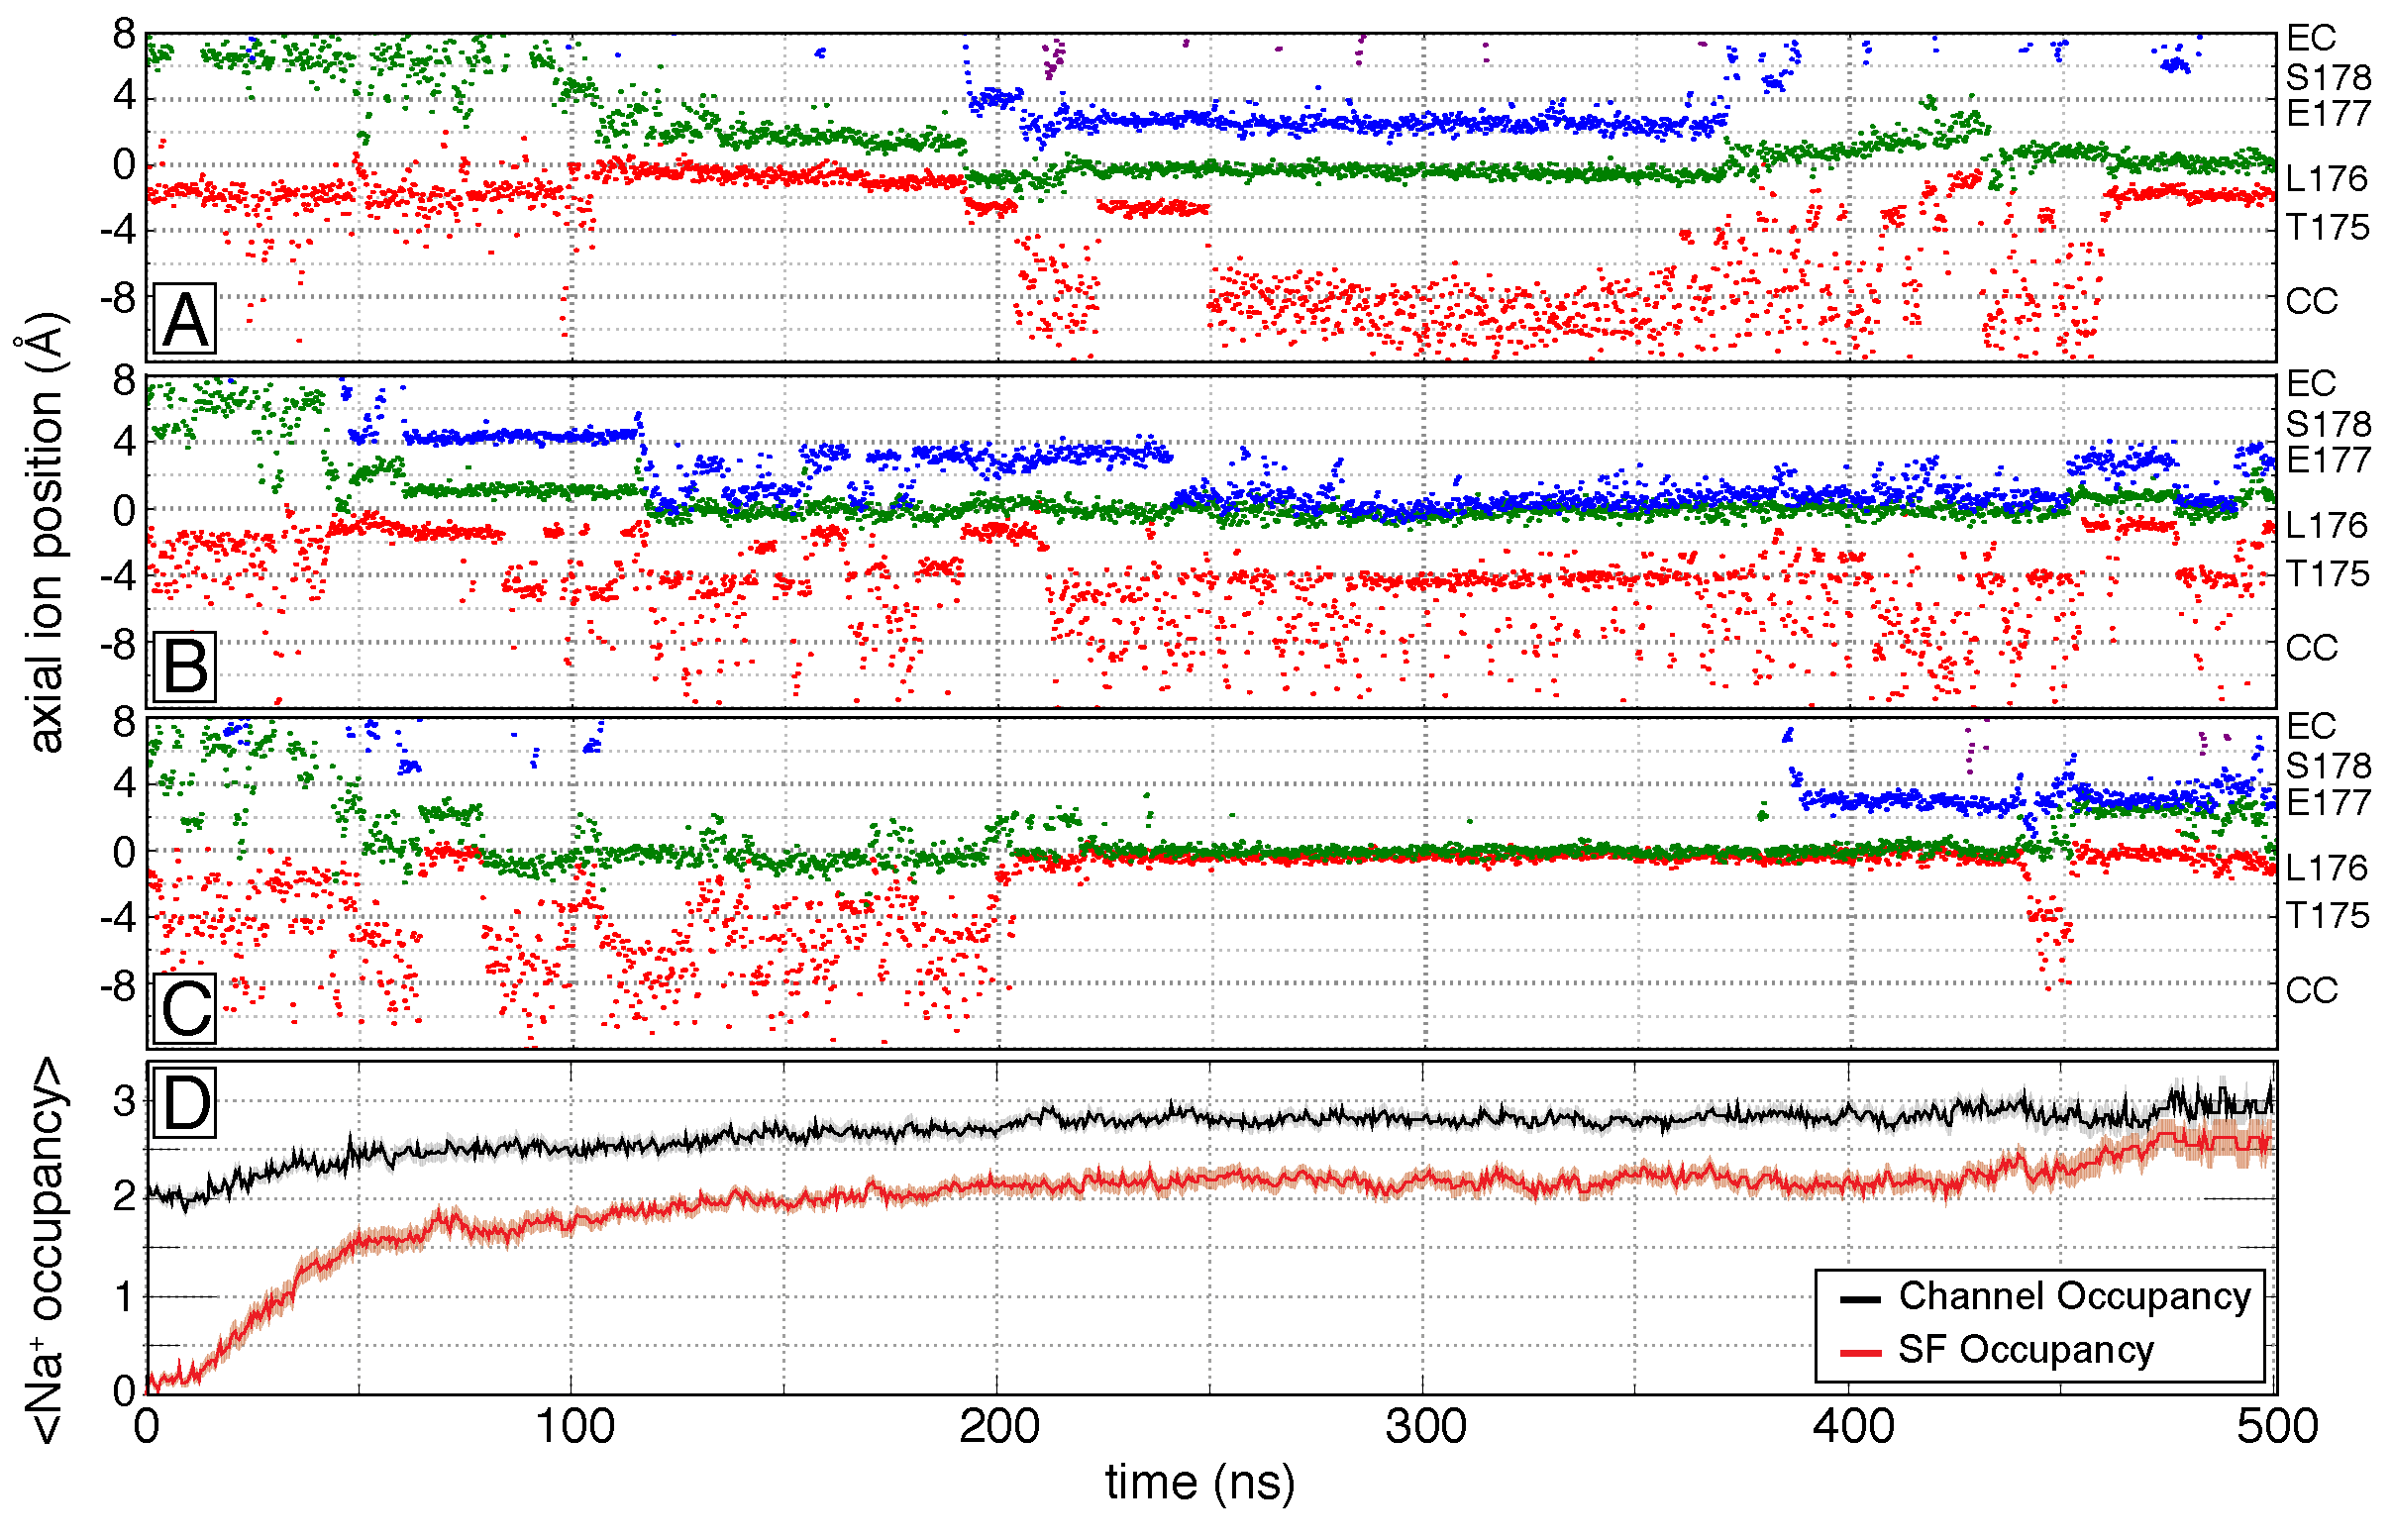
\includegraphics[width=0.9\textwidth]{navreview/revfig2}
\caption[Time series of axial Na$^{+}$ positions and average occupancy from unbiased equilibrium simulations of NavAb]{\textbf{Time series of axial Na$^{+}$ positions and average occupancy from unbiased equilibrium simulations of NavAb} (Chakrabarti et al. 2013). (\textbf{A-C}) Three out of forty-seven simulation repeats, where Na$^{+}$ reversibly diffuse in and out of the SF.  Na$^{+}$ cations are colored by depth rank within the SF from intracellular to extracellular (ordered red, green, blue in color, or lightest to darkest in grayscale).  The channel was initially devoid of cations and simulations differed in initial random velocities. (\textbf{D}) Time dependence of average Na$^{+}$ occupancy across all forty-seven simulation repeats for the channel (black, defined as any Na$^{+}$ within axial range 8 $\angstrom$ to -12 $\angstrom$) and SF (red, defined as any Na$^{+}$ with first-shell coordination to channel ligands E177 and L176).  Error bars are computed using the standard error of mean across all simulation repeats.  The simulation length of individual repeats varied from 450 to 500 ns, resulting in a smaller data set and increased noise in the last 50 ns of this time series.}
\label{fig:rev2}
\end{figure}

Although biased-sampling methods have been used to quantify the favorable binding sites of Na$^{+}$ and K$^{+}$ in the Nav channel SF, extensive unbiased equilibrium simulations have not been performed in the study of ionic selectivity.  In the field-strength model of K$^{+}$ selectivity by Noskov et al., it was suggested that the number and the type of ligands could directly influence selectivity \cite{Noskov:2006fd,Noskov:2004tv}. This model is interesting when viewed in the context of Nav channels, since conformational isomerization of E177 side chains may result in a variable number of coordinating ligands.  Chakrabarti et al. observe an average SF occupancy of $2.09 \pm 0.05$ Na$^{+}$ cations coordinated by an average of $2.23 \pm 0.04$ carboxylate groups, whereas the average SF occupancy of K$^{+}$ and its average coordinate to carboxylate side chains is yet to be determined \cite{Chakrabarti:2013kd}.  Simulations by Ngo et al. suggest that carboxylate coordination contributes to K$^{+}$ blockage during inward conduction, but they did not explicitly study the effect of conformational isomerization with respect to selectivity of Na$^{+}$ \cite{Ngo:2016es}.  Using biomimetic graphene pores containing carboxylate or carbonyl groups, He et al. studied the voltage dependence of Na$^{+}$ and K$^{+}$ currents as well as selectivity \cite{He:2013it}.  A graphene pore with three carboxylate groups was found to be Na$^{+}$-selective at low voltage and K$^{+}$-selective at high voltage in mixed-cation solutions.  Voltage was also found to induce conformational changes in carboxylate group orientation with respect to the direction of the electric field, with an out-facing state associated with K$^{+}$ selectivity and and lumen-facing state associated with Na$^{+}$ selectivity.  While there are many differences between such simplified models and the complex environment of the SF of Nav channels, this study supports a putative mechanism of selectivity involving the conformational isomerization of E177 side chains that remains to be examined in Nav channels.
 
 In Nav channels, multi-microsecond simulations have yet to be used to study the selectivity of Na$^{+}$ over Ca$^{2+}$. In addition to long simulation timescales, polarizable force fields may be required to reach quantitative estimates of Na$^{+}$:Ca$^{2+}$ conductance ratios that match experimental values.  Because the ionic radii of Na$^{+}$ and Ca$^{2+}$ are very similar (1.16 \angstrom and 1.14 \angstrom, respectively), an accurate treatment of Ca$^{2+}$ requires the use force fields that account for electronic polarization in the environment surrounding the ion, since the valence charge is greater for Ca$^{2+}$ \cite{Huang:2014ia}. Non-polarizable models of Ca$^{2+}$ fail to reproduce protein-ion binding energies from using quantum mechanical calculations over a diverse range of cation binding sites \cite{Ngo:2015ki}. It has been shown that electronic polarization results in significant ion-induced dipole shifts on the carbonyl groups of the SF in KcsA \cite{Allen:2006jw,Bucher:2009ef}, but this effect is unknown in Nav channels.  As such, quantitative estimates from Nav channel simulations of Ca$^{2+}$ using non-polarizable force fields must be considered carefully.
 
 \section{Perspectives}
 Computational studies of bacterial Nav channels offer a unique perspective on molecular mechanisms of ionic permeation in a weakly-selective channel.  The consensus mechanism of Na$^{+}$ permeation consists of a weakly-coupled knock-on involving approximately two ions on average.  Multiple studies have described the lowest-energy, two-ion occupancy state of the SF as one in which ions are partially dehydrated and bind the SF in off-axis fashion in an upper site (S$_{HFS}$) and a lower site (S$_{CEN}$ and/or S$_{IN}$).  Permeation occurs via these two sites with low ($\sim$1-2 kcal/mol) intervening free energy barriers and the cations are able to pass one another, with occasional double occupancy of one or more sites in the SF.  Although no consensus model of Na$^{+}$ selectivity has yet been established, several proposed mechanisms attribute selectivity to high permeation barriers between upper and lower binding sites for K$^{+}$ and Ca$^{2+}$.  
In qualitative agreement with experiment, most of the simulation studies of cation permeation in Nav channels published to this date support a rapid conduction process.  Equilibrium simulations of Na$^{+}$ in NavAb yielded estimates of permeation rates with the correct order of magnitude for a sodium channel \cite{Chakrabarti:2013kd}.  Estimates of Na$^{+}$ conductance computed from two non-equilibrium studies were in good agreement with experimental values \cite{Ke:2014fy,Ulmschneider:2013da}.  One of these studies also reported a Na$^{+}$:K$^{+}$ conductance ratio commensurate with experimental measurements, while all other studies of Na$^{+}$ selectivity over K$^{+}$ and Ca$^{2+}$ were qualitatively correct.  Future studies of ionic selectivity in Nav channels will benefit from more comprehensive sampling of different ionic species in order to assess the importance of conformational isomerization of Glu side chains in this process.  In an effort to reproduce experimental selectivity ratios, it would be useful to conduct simulations of Nav channels in bi-ionic conditions in the presence of applied voltage to compute reversal potentials.
In order to obtain simulation results that are minimally biased by systematic and statistical error, we suggest performing multiple repeats of unbiased equilibrium simulations as the optimal approach.  Individual simulations should be long enough to observe SF conduction events (requiring computational resources accessible on non-specialized supercomputers), with improved sampling due to randomized initial velocities and positions that may sample more uncorrelated ion binding modes than single long-time simulations.  Equilibrium simulations (with 0 mV applied voltage) are a good approximation to the low physiological voltages associated ion conduction \cite{Hille:2001tw}, but non-equilibrium simulations may also be used in the limit of low applied voltage in the physiological regime.  When biased sampling approaches are utilized, accelerated sampling algorithms such as bias-exchange metadynamics offer some benefits over umbrella sampling \cite{Domene:2015kj}. However, even these approaches would benefit from multiple simulation repeats to ensure that infrequent structural transitions involving other degrees of freedom, such as conformational isomerization of E177 side chains, are appropriately sampled, failing which, reaction coordinates including channel degrees of freedom could be considered.
One important issue that must be considered in evaluating simulations is that they have been performed using different simulation methodologies (biased, unbiased equilibrium, and unbiased non-equilibrium sampling), different force fields (CHARMM, AMBER, OPLS), different channel structures (closed and open conformations), and different simulation conditions (such as temperature, ionic concentration, and applied voltage) (Tables \ref{table:biased}, \ref{table:unbiased}). For Na$^{+}$ channels, these differences result in discrepancies in estimates of ion binding, permeation, and selectivity.  Dataset sizes varied between 0.1 and 10 microseconds of aggregate sampling between studies, and as such, it is not realistic to expect a consensus on the details of permeation and selectivity.  In general, continued progress in computer simulation studies of ion channels will greatly benefit from the quantification of both systematic and statistical errors. 
 
 
\printbibliography[heading=subbibnumbered,title={References}]
 \end{refsection}
\begin{refsection}
\chapter{Multi-ion Effects and Na$^+$ Selectivity over K$^+$ in Sodium Channel Na\textsubscript{V}Ab}

Contributions by Christopher Ing (CI) and Regis Pomes (RP): C.I. and R.P. designed the research. Simulations were performed by C.I. Data analysis was performed by C.I. and R.P. The manuscript was written by R.P. and C.I.

\newpage

\section{Summary}

The structural determination of the prokaryotic voltage-gated sodium channel Na\textsubscript{V}Ab has enabled the elucidation of the molecular determinants of cation permeation and selectivity.  To examine the microscopic basis for selectivity of Na\textsubscript{V}Ab for Na$^+$ over K$^+$, we generated dozens of 1000-ns molecular dynamics trajectories in the presence of NaCl, KCl, or a mixture of the two. Na$^+$ and K$^+$ bind in similar ways in the selectivity filter of Na\textsubscript{V}Ab, with multiple binding modes involving a variable number of cations and flexible E177 side chains. Na$^+$ movement through the selectivity filter is coupled to the conformational isomerization of E177 between out-facing and lumen-facing rotamers. Na$^+$ conduction proceeds through a loosely-coupled knock-on mechanism involving an interconversion between 2 and 3 bound ions within the selectivity filter, lowering the free energy for Na$^+$ conduction. K$^+$ conduction proceeds through a single-file knock-on mechanism with relatively static binding sites. In mixed cation simulations, Na$^+$ is favored over K$^+$ at primary binding sites by a factor of 2-3. Modifications to the EEEE ring of the selectivity filter with artificial conformational restraints, the E177D mutation, or E177 protonation, dramatically alter selectivity, supporting E177 as a critical determinant for Na$^+$ selectivity in bacterial Nav channels.

\section{Introduction}

Ion channels of excitable cells can be highly selective, but the structural basis of selectivity remains unclear \cite{Hille:2001tw}.   Based on the crystal structure of the K$^+$ channel KcsA \cite{Doyle:1998wq}, the 104-fold  preference of that channel for K$^+$ over Na$^+$ was first explained by invoking the snug-fit model \cite{Bezanilla:1972uz}, in which the selectivity filter (SF) of the channel is essentially rigid.  However, molecular dynamics (MD) simulations of KcsA \cite{Guidoni:1999ba} subsequently showed that the SF of KcsA is flexible \cite{Andersen:2011ty}, igniting a debate on the role of structural fluctuations of the protein in ionic selectivity.  Various theoretical models have been employed in the past decade in an effort to elucidate the molecular determinants for the selectivity of K$^+$ over Na$^+$ in KcsA, emphasizing the balance of ion-channel and channel-channel interactions \cite{Noskov:2004tv} as well as the spatial constraints imposed on the SF by the protein fold \cite{Andersen:2011ty,Bostick:2010bm,Dixit:2011wf,Roux:2011ed,Varma:2011gn}. The role of both equilibrium and kinetic factors in selectivity is thought to be essential for the NaK channel, based on electrophysiological measurements of two single-point mutants, one of which was found to be selective and the other non-selective despite both channels being reported as K$^+$ selective over Na$^+$ at equilibrium on the basis of isothermal titration calorimetry and crystallographic titration \cite{Liu:2013hf,Sauer:2013gk}. 

While the molecular basis of ionic selectivity in K$^+$ channels is still under debate, even less is known about Na$^+$ selectivity.  The recent elucidation of the structures of bacterial voltage-gated Na$^+$ channels Na\textsubscript{V}Ab \cite{Payandeh:2012ib,Payandeh:2013ex}, NavMs \cite{McCusker:2012di} NavAep1 \cite{Shaya:2014gg}, and NavRh \cite{Zhang:2013bz} provides a structural basis for answering that question. The molecular structure of the SF of Na\textsubscript{V}Ab (TLESW) is both wider and shorter than that of K$^+$ channels such as KcsA (TVGYG).  In KcsA, channel coordination of permeating cations consists entirely of direct interactions with backbone carbonyl oxygen atoms, whereas in Na\textsubscript{V}Ab, the SF is lined with amino acid side chains from S178 and E177 in addition to backbone carbonyl groups from T175 and L176 \cite{Doyle:1998wq,Payandeh:2012ib,Jiang:2003vh}.  Due to the tetrameric domain arrangement of Na\textsubscript{V}Ab, the E177 site forms a ring of four glutamate side chains (EEEE) in the same sequence positions as the characteristic DEKA ring of eukaryotic sodium channels \cite{Heinemann:1992ep,Terlau:1991ud}. Simulation studies have revealed that dynamic fluctuations of these four glutamic acid side chains can effectively modulate the diameter of the SF as ions bind and diffuse through it \cite{Boiteux:2014ut,Chakrabarti:2013kd}. In contrast with strongly selective K$^+$ channels, this raises the question of how a wider and more flexible SF could result in a weakly selective channel, on the order of 10:1 for Na$^+$ over K$^+$ \cite{Payandeh:2012ex,Ulmschneider:2013da}. 

Recent MD studies have examined the conduction of Na$^+$ and K$^+$ in bacterial voltage-gated Na$^+$ channels \cite{Boiteux:2014ut,Corry:2012ge,Domene:2015kj, FinolUrdaneta:2014bz,Furini:2012jl,Ngo:2016es,Ulmschneider:2013da,Chakrabarti:2013kd}. Na$^+$ conduction was found to occur through a loosely coupled knock-on mechanism, whereby an incoming Na$^+$ causes an ion bound within the SF to move into the central cavity (CC), but wherein the movement of both ions are not necessarily concerted. Unbiased and biased sampling techniques have been used to compute the lowest free-energy conduction pathway for multiple Na$^+$ or K$^+$ within the SF, identifying regions within the SF that were selective. Across several of these studies, Na$^+$ and K$^+$ were found to bind at similar sites within the SF, with different relative affinities \cite{Ing:2016em}. In a study utilizing unbiased non-equilibrium simulations \cite{Ulmschneider:2013da}, the computed Na$^+$:K$^+$ selectivity, based on a ratio of conductance, was found to be in agreement with experimental values. However, no study has described a molecular mechanism for Na$^+$ selectivity involving three ion occupancy of the SF, nor has such a mechanism been described on the basis of unbiased equilibrium studies at physiological voltages. 

Among the previous Nav channel studies, our analysis showed that E177 side chains are essential ligands of Na$^+$ and that their conformational isomerization is coupled to binding and movement of Na$^+$ \cite{Chakrabarti:2013kd}. Multiple studies have since analyzed the role of glutamic acid sidechain fluctuations in Na$^+$ conduction \cite{Boiteux:2014ut,Domene:2015kj,Furini:2014gv,Ke:2014fy}. A similar mechanism has been discovered in the glutamate ring of the cation-selective nicotinic acetylcholine receptor \cite{Harpole:2014gu}. These findings raise the question of the role of Glu binding and dynamics in ion selectivity of Na\textsubscript{V}Ab and other Na$^+$-selective channels. Experimental measurements reveal that both the side-chain shortening mutation E177D and lowering the pH can modulate Na$^+$ over K$^+$ selectivity in the channel NaChBac \cite{FinolUrdaneta:2014bz}. In the experiments presented here, we follow up our previous studies of Na$^+$ permeation in Na\textsubscript{V}Ab \cite{Chakrabarti:2013kd} with experiments on K$^+$ permeation in isolation and on Na$^+$ and K$^+$ permeation in competition with each other. We compare permeation in four closed-channel systems; the wildtype (WT) channel, WT with conformational restraints on the E177 side chain, the E177D mutant, and WT with a single protonated E177 side chain. In order to examine the reversible diffusion of ions in and out of the SF, as well as competitive binding, we generated ten to twenty 1000-ns trajectories for each system in the presence of NaCl, KCl, and a mixture of the two, for a total sampling time of 200 $\mu$s. To test the generality of our findings and to understand the extent to which systematic errors can alter ion binding properties, we repeated NaCl and KCl simulations using the WT channel system with four alternate force fields. Across several force fields, our results show that selectivity emerges due to a dynamic fluctuations of the SF favoring Na$^+$ over K$^+$. A loosely-coupled knock-on mechanism, facilitated by E177 side chains, results in a diffusive energy landscape for Na$^+$ but not for K$^+$, manifesting as a selective advantage for Na$^+$ in mixed cation simulations. 

\section{Results}

\subsection{Na$^+$ and K$^+$ Ions in the Na\textsubscript{V}Ab Pore}

\begin{figure}[!ptb]
\centering\
\includegraphics[width=0.8\textwidth]{nav2/Nav2Fig1}
\caption[Sodium and potassium ion movement in the selectivity filter of Na\textsubscript{V}Ab]{\textbf{Sodium and potassium ion movement in the selectivity filter of Na\textsubscript{V}Ab}. (\textbf{A}) Representative snapshots of Na$^+$ and K$^+$ (spheres) in the SF sampled from two time trajectories.  Ions are colored red, green, and blue from the bottom (intracellular end) to the top (extracellular) in the channel.  The pore-lining oxygen groups of the SF (backbone carbonyl groups of T175 and L176 and the side chains of E177 and S178) are shown. Water molecules are not shown.  (\textbf{B, D}) Movement of Na$^+$ or K$^+$ cations along the pore axis from selected simulation repeats. (\textbf{C, E}) Distribution of Na$^+$ or K$^+$ along the pore axis over all simulation repeats, with colored sub-distributions representing the coordination groups of a permeating ion at that axial position. Colored bars at the bottom of time series (\textbf{B}) and (\textbf{D}) indicate the channel occupancy state (legend in top right).}
\label{fig:nav2fig1}
\end{figure}

Figure \ref{fig:nav2fig1} depicts two MD time trajectories obtained in presence of either NaCl (Fig. \ref{fig:nav2fig1} B) or KCl (Fig. \ref{fig:nav2fig1} D) in the closed state of Na\textsubscript{V}Ab (PD+VSD model, pore domain and voltage sensors, Fig. \ref{fig:nav2figS1}). Molecular renderings at different time points show that ions occupying the SF can be coordinated to a variable number of glutamic acid side chains (Fig. \ref{fig:nav2fig1} A). We observe reversible diffusion of Na$^+$ and K$^+$ in and out of the SF, with total channel occupancy that fluctuates between two (Fig. \ref{fig:nav2fig1} A i,v) and three ions (Fig. \ref{fig:nav2fig1} A ii-iv), labelled along the time trajectories by yellow and purple bars, respectively (Fig. \ref{fig:nav2fig1} B,D). In the three ion occupancy state, two Na$^+$ may reside at nearly the same axial position ($\sim$850 ns in Fig. \ref{fig:nav2fig1} B), but K$^+$ did not adopt this configuration, remaining in a single-file arrangement. At several points along the time trajectory, regardless of the total channel occupancy, the innermost ion (in red) moves in and out of the central cavity (CC). Sequential movement of Na$^+$ or K$^+$ may occur through a concerted knock-on mechanism, whereby an outer ion displaces the innermost ion into the CC ($\sim$650 ns for Na$^+$, $\sim$350 ns for K$^+$, in Fig. \ref{fig:nav2fig1} B,D, respectively). Similarly, ion permeation may also occur through a loosely-coupled knock-on mechanism, whereby the innermost ion enters the CC without requiring the entry of a new ion into the SF ($\sim$860 ns for Na$^+$, $\sim$750 ns for K$^+$ in Fig. \ref{fig:nav2fig1} B,D, respectively). 

\begin{figure}[!ptb]
\centering
\includegraphics[width=0.7\textwidth]{nav2/Nav2FigS4}
\caption[Binding modes of Na$^+$ or K$^+$ along the pore axis]{\textbf{Binding modes of Na$^+$ or K$^+$ along the pore axis}. Total ionic distributions are shown for Na$^+$ (blue solid line; left half panel) and K$^+$ (green solid line; right half panel) with colored sub-distributions identifying the groups of channel oxygens coordinating an ion at that axial position. Binding modes are defined by coordination to one or more channel ligands in either the first or second coordination shell (S178-only, E177-only, E177 and L176, L176 and T175, or no coordination in the central cavity). A gold band indicates the region of highest free-energy barrier for K$^+$ permeation within the SF. Distributions are normalized by channel average channel occupancy.}
\label{fig:nav2figS4}
\end{figure}

The axial distribution of ion positions averaged across all simulation repeats indicates that Na$^+$ and K$^+$ differ in E177 (`E') and combined E177/L176 (`EL') coordination, but share a very similar L176/T175 (`LT') binding site (Fig. \ref{fig:nav2fig1} C,E). The distribution of ions in the `E' and `EL' binding modes are broad and strongly overlap for Na$^+$ but not for K$^+$, which is sharply localized at non-overlapping sites. Similar features are observed in a pore-domain only (PD model) with pure NaCl or KCl solutions (Fig. \ref{fig:nav2figS4} C). The average occupancy of the pore is similar across all pure-NaCl and pure-KCl simulations ($2.2 \pm 0.1$ for Na$^+$ and $2.5 \pm 0.1$ for K$^+$, Fig. \ref{fig:nav2fig2} B). The most significant difference between the two solutions is that two Na$^+$ cations occupy the `EL' binding site in $11.33 \pm 0.04$\% frames. Although a large number of ionic arrangements were sampled within the SF, dual ion occupancy of the `EL' site occurs most frequently in conjunction with single occupancy of the `E' site (Figs. \ref{fig:nav2fig1} A iii, \ref{fig:nav2fig2} C).  The most populated ionic arrangements of NaCl and KCl simulations, accounting for 84.1\% and 89.2\% of frames, respectively, suggest that the two cations differ in that the SF can accommodate multiple Na$^+$ at similar axial positions near the `E' and `EL' sites, but that K$^+$ must traverse the SF in a single-file arrangement. 

\begin{figure}[!ptb]
\centering
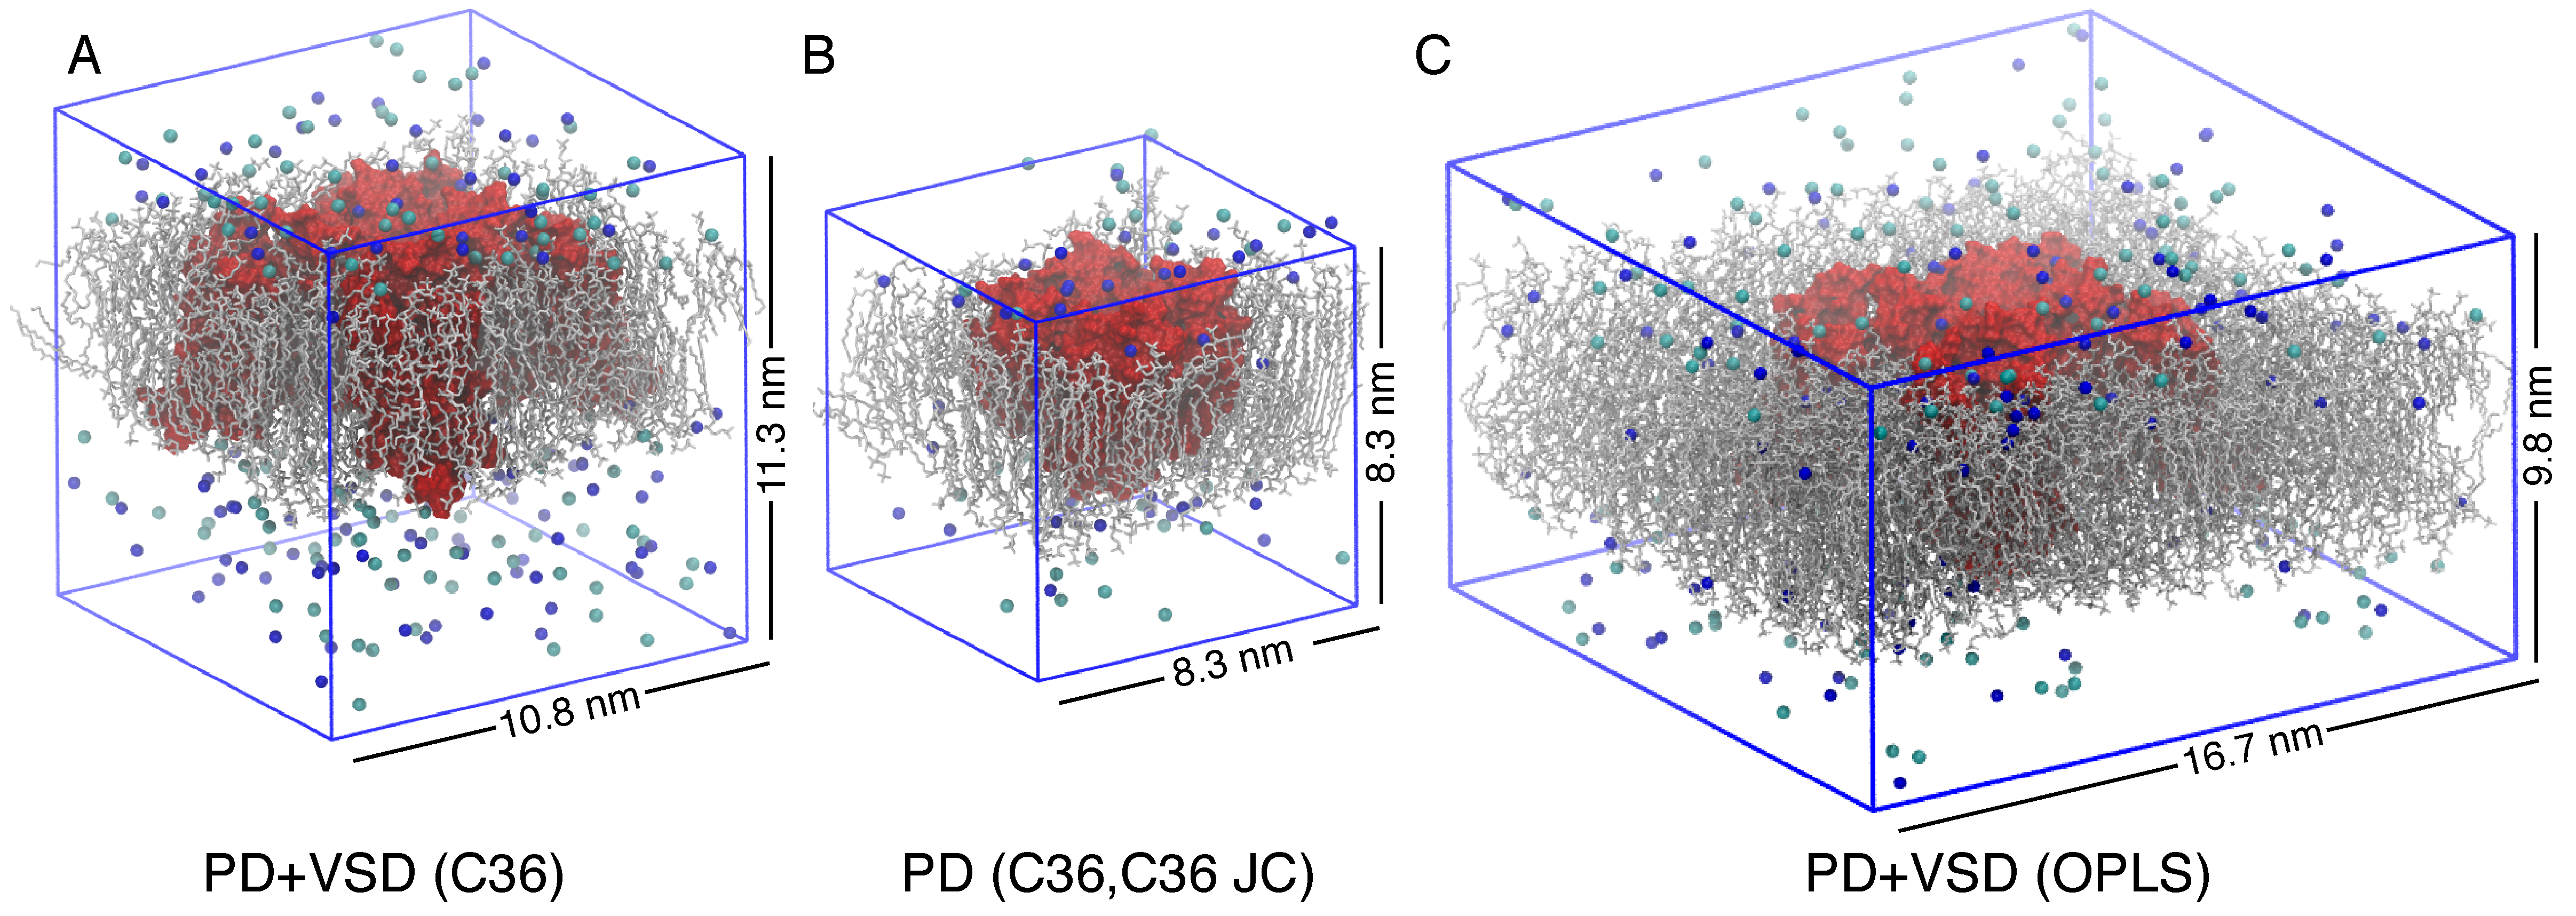
\includegraphics[width=0.9\textwidth]{nav2/Nav2FigS1}
\caption[Molecular models of Na\textsubscript{V}Ab in a hydrated lipid bilayer]{\textbf{Molecular models of Na\textsubscript{V}Ab in a hydrated lipid bilayer}. Initial models of the (\textbf{A}) full channel including pore domain and voltage-sensing domains (PD+VSD), (\textbf{B}) pore domain-only model (PD) prepared for NaCl simulations, and (\textbf{C}) full channel with an alternate simulation force field (PD+VSD, OPLS). Na\textsubscript{V}Ab protein is rendered as a surface (red) with DMPC molecules shown in grey licorice representation. Na$^+$ and Cl- are shown as blue and aqua spheres, respectively, and water is not shown. }
\label{fig:nav2figS1}
\end{figure}

\subsection{Conformational Isomerization of Glu side chains}
In pure Na$^+$ and K$^+$ simulations, conformational isomerization of E177 side chains occurs spontaneously and reversibly. We have previously described how  Na$^+$ movement is coupled to the conformational isomerization of the side chains of E177, which is captured by dynamic changes in the number of conformationally flipped or `dunked' side chains \cite{Chakrabarti:2013kd}. Specifically, cation binding shifts the conformational equilibrium of E177 from the crystallographically-observed conformer, ($\chi_1$,$\chi_2$) = (t, g+), in which the carboxylate group points towards the EC mouth (Fig. \ref{fig:nav2fig2} A, yellow circle), to ($\chi_1$,$\chi_2$) = (t, g-), where the carboxylate group points into the lumen (Fig. \ref{fig:nav2fig2} A, purple circle) \cite{Chakrabarti:2013kd}.  An average of $2.1\pm 0.1$ and $2.0\pm  0.1$ carboxylate side chains adopt a lumen-facing conformation, for NaCl and KCl respectively. Isomerization of these side chains result in near charge compensation, directly coordinating an average of $2.0\pm0.1$ cations, for both NaCl and KCl (Fig. \ref{fig:nav2fig2} B). In the two time trajectories shown in Figure \ref{fig:nav2fig1}, the time series of the axial center of cationic and anionic charge have a Pearson correlation of YY and ZZ for Na$^+$ and K$^+$ simulations, respectively, indicating that Glu side chain dynamics is coupled to ion movement. 

\begin{figure}[!htb]
\centering
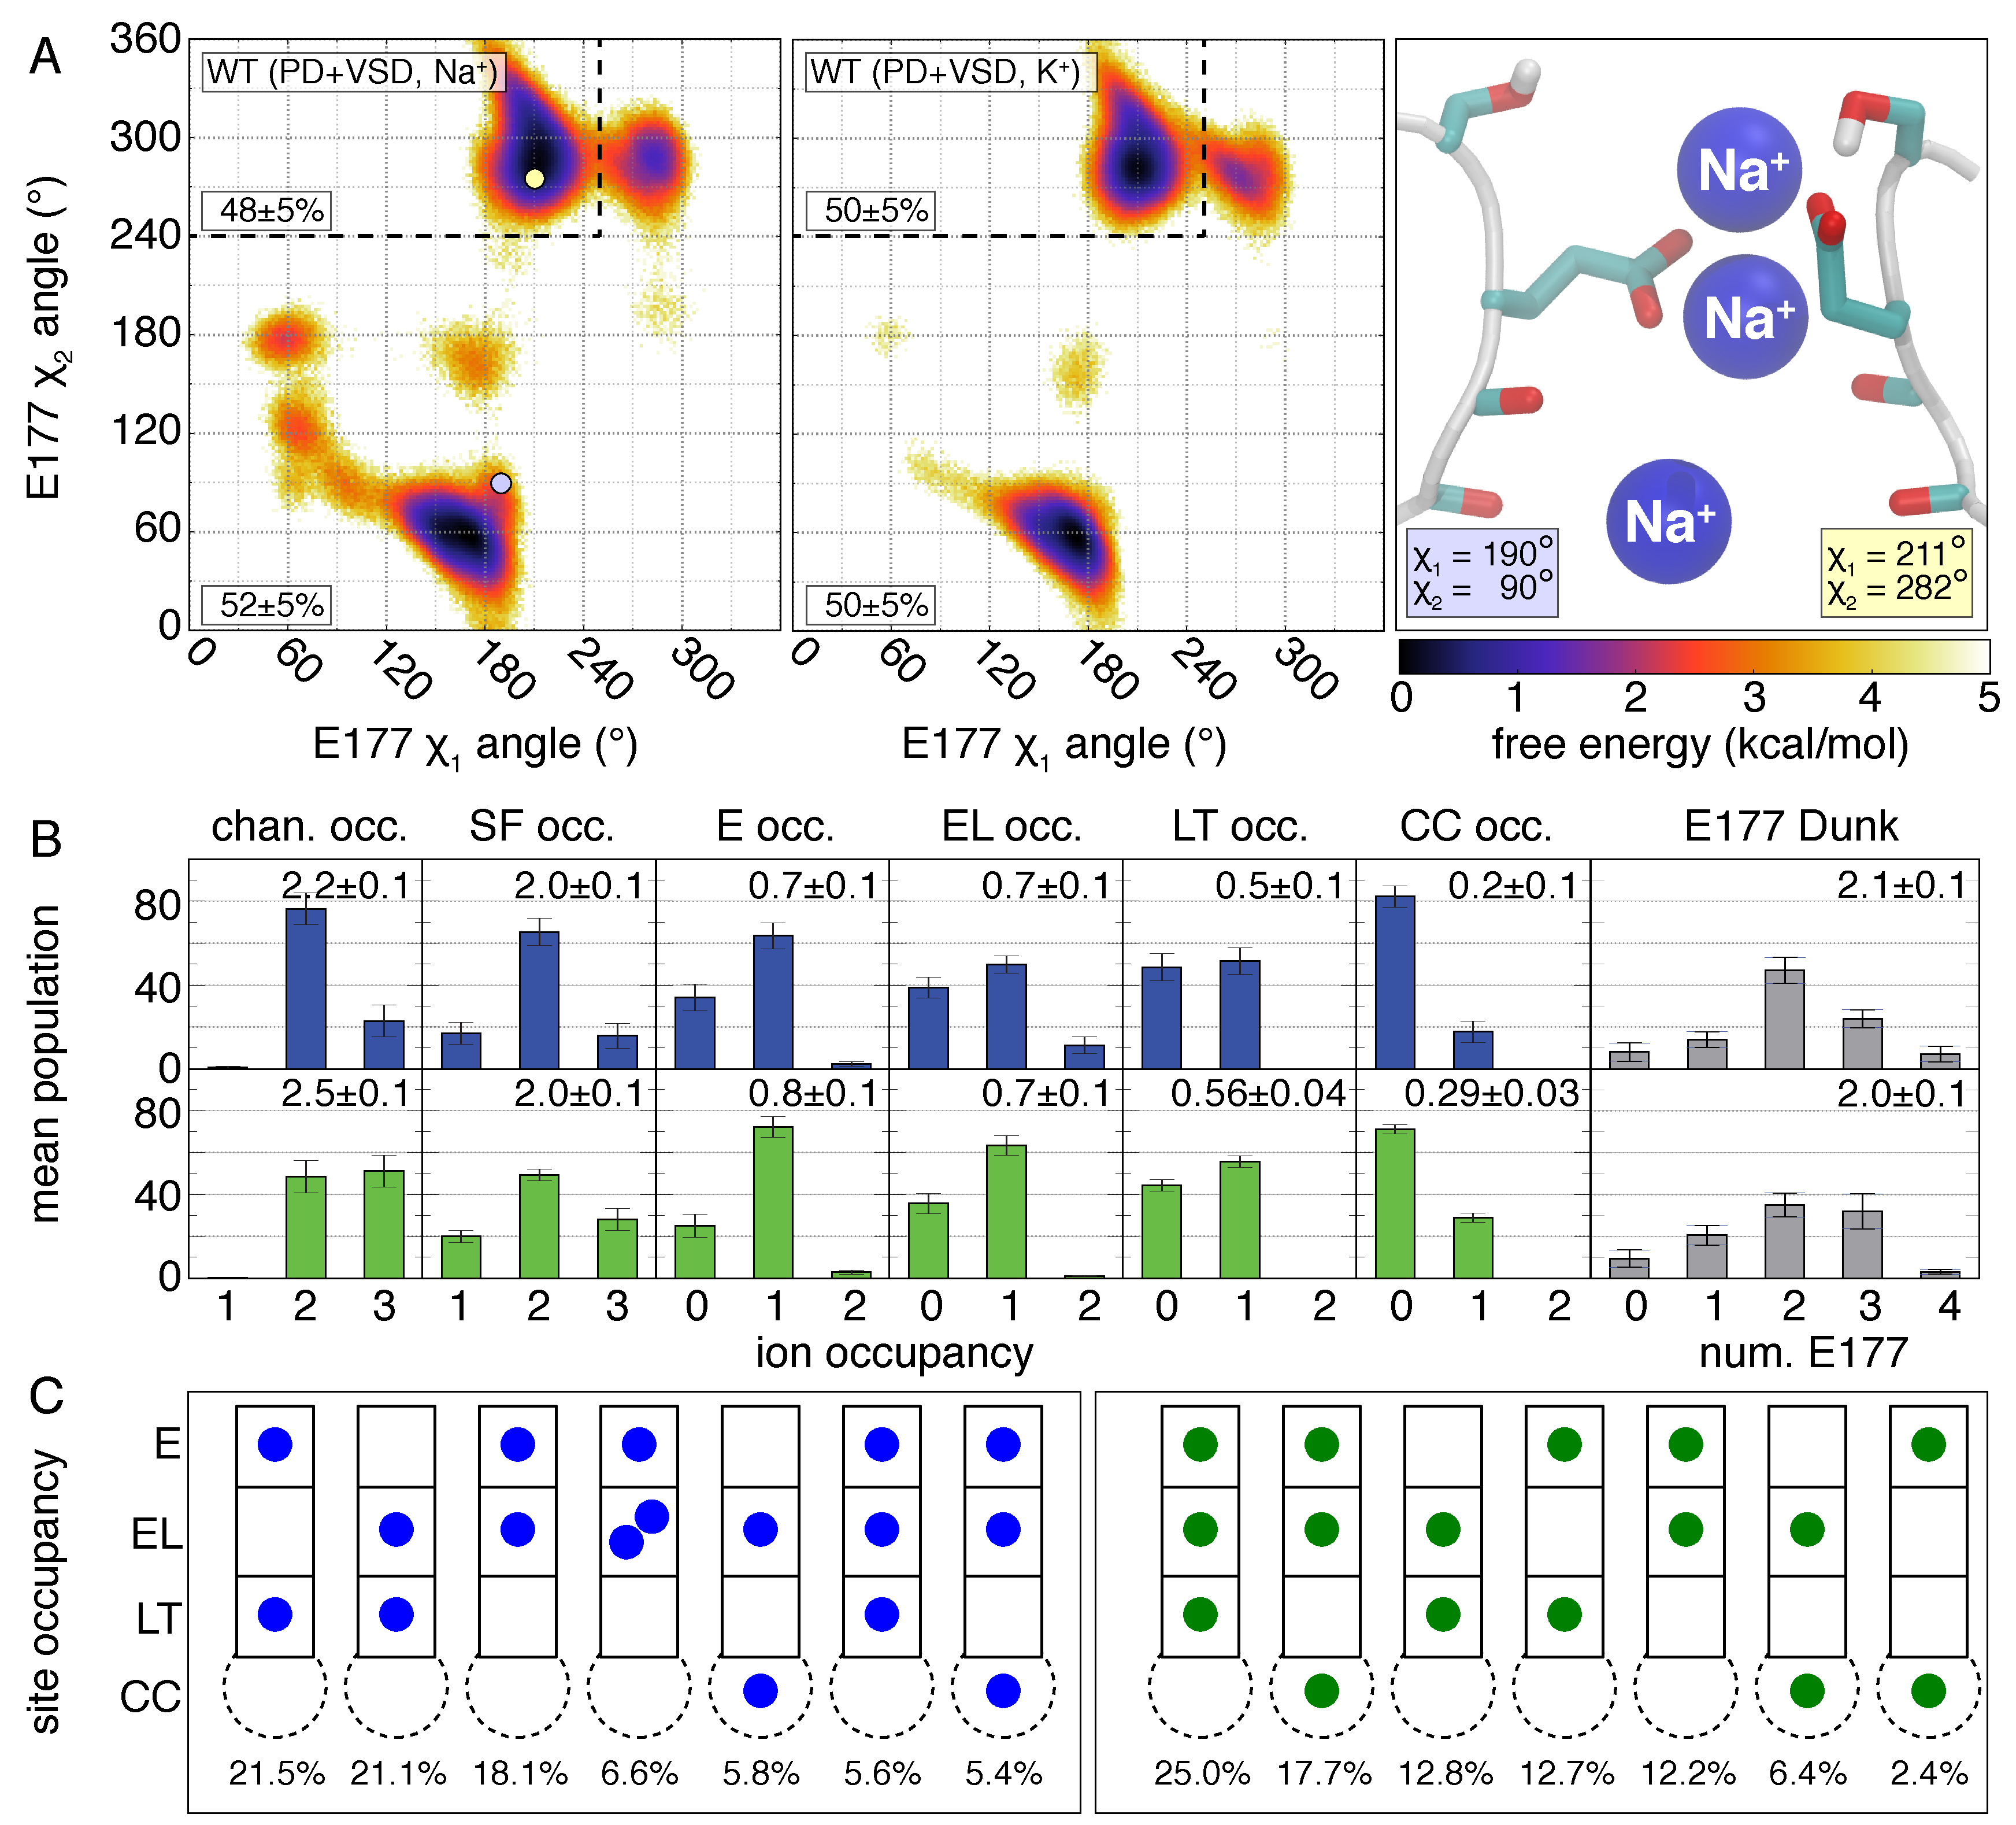
\includegraphics[width=0.7\textwidth]{nav2/Nav2Fig2}
\caption[Conformational isomerization of E177 side chains and ion binding statistics]{\textbf{Conformational isomerization of E177 side chains and ion binding statistics}. (\textbf{A}) Probability distribution of cation binding and E177 side-chain isomerization across all MD trajectories, for Na$^+$ (blue) and K$^+$ (green) in the PD+VSD model. (\textbf{A}) Free energy profiles for ($\chi_1$, $\chi_2$) of E177 in the PD+VSD model for pure Na$^+$ and K$^+$ ion concentrations, as well as pure Na$^+$ in the PD model with E177 dihedral restraints on all chains. Colored circles indicate the ($\chi_1$, $\chi_2$) value of the molecular rendering (right), and in-set boxes show the total percentage of data in two regions of $\chi_1$, $\chi_2$ space, corresponding to `undunked' and `dunked' conformations from top to bottom. (\textbf{B}) Ionic occupancy is shown from left to right for the entire channel, the SF, and for all major binding sites within the SF defined by 1st and 2nd shell coordination, together with the number of dunked E177 side chains. (\textbf{C}) Ionic occupancy of binding sites (E, EL, LT, CC) in the highest population channel configurations for pure Na$^+$ and K$^+$. Populations over all simulation repeats are shown below each state.}
\label{fig:nav2fig2}
\end{figure}

\subsection{Free Energy of Ion Permeation in the SF}

Two-dimensional potential of mean force (PMF) plots are shown for distinct ion pairs in order to identify the lowest free energy pathways for Na$^+$ and K$^+$ conduction (Fig. \ref{fig:nav2fig3}). Since dual occupancy of `EL' by Na$^+$ is dependent on the occupancy of the SF, free energy profiles are calculated separately for two (Fig. \ref{fig:nav2fig3} A-B) and three ion occupancies (Fig. \ref{fig:nav2fig3} C-H). The most populated channel occupancy state for both Na$^+$ and K$^+$, 2, involves the red and green ions adopting multiple configurations in the `E', `EL', and `LT' sites (Fig. 3A-B). For both Na$^+$ and K$^+$, the innermost ion (red), is primarily localized at the `LT' site ($\sim$4 \AA), but is capable of sampling a broad range of positions from 0 to $\sim$8 \AA. With two ions in the SF, the outermost ion (green) exchanges between the `E' and `EL' binding sites for both Na$^+$ and K$^+$, localized within the axial range of -4 to 0 \AA. However, a green Na$^+$ moves relatively unimpeded between `E' and `EL' binding sites, whereas a green K$^+$ resides at the `E' or `EL' sites, separated by a free energy barrier on the order of $\sim$1 kcal/mol. For both Na$^+$ and K$^+$, entry of the red ion into the CC occurs with highest propensity when the green ion holds a position near 0 \AA. 

\begin{figure}[hp]
\centering
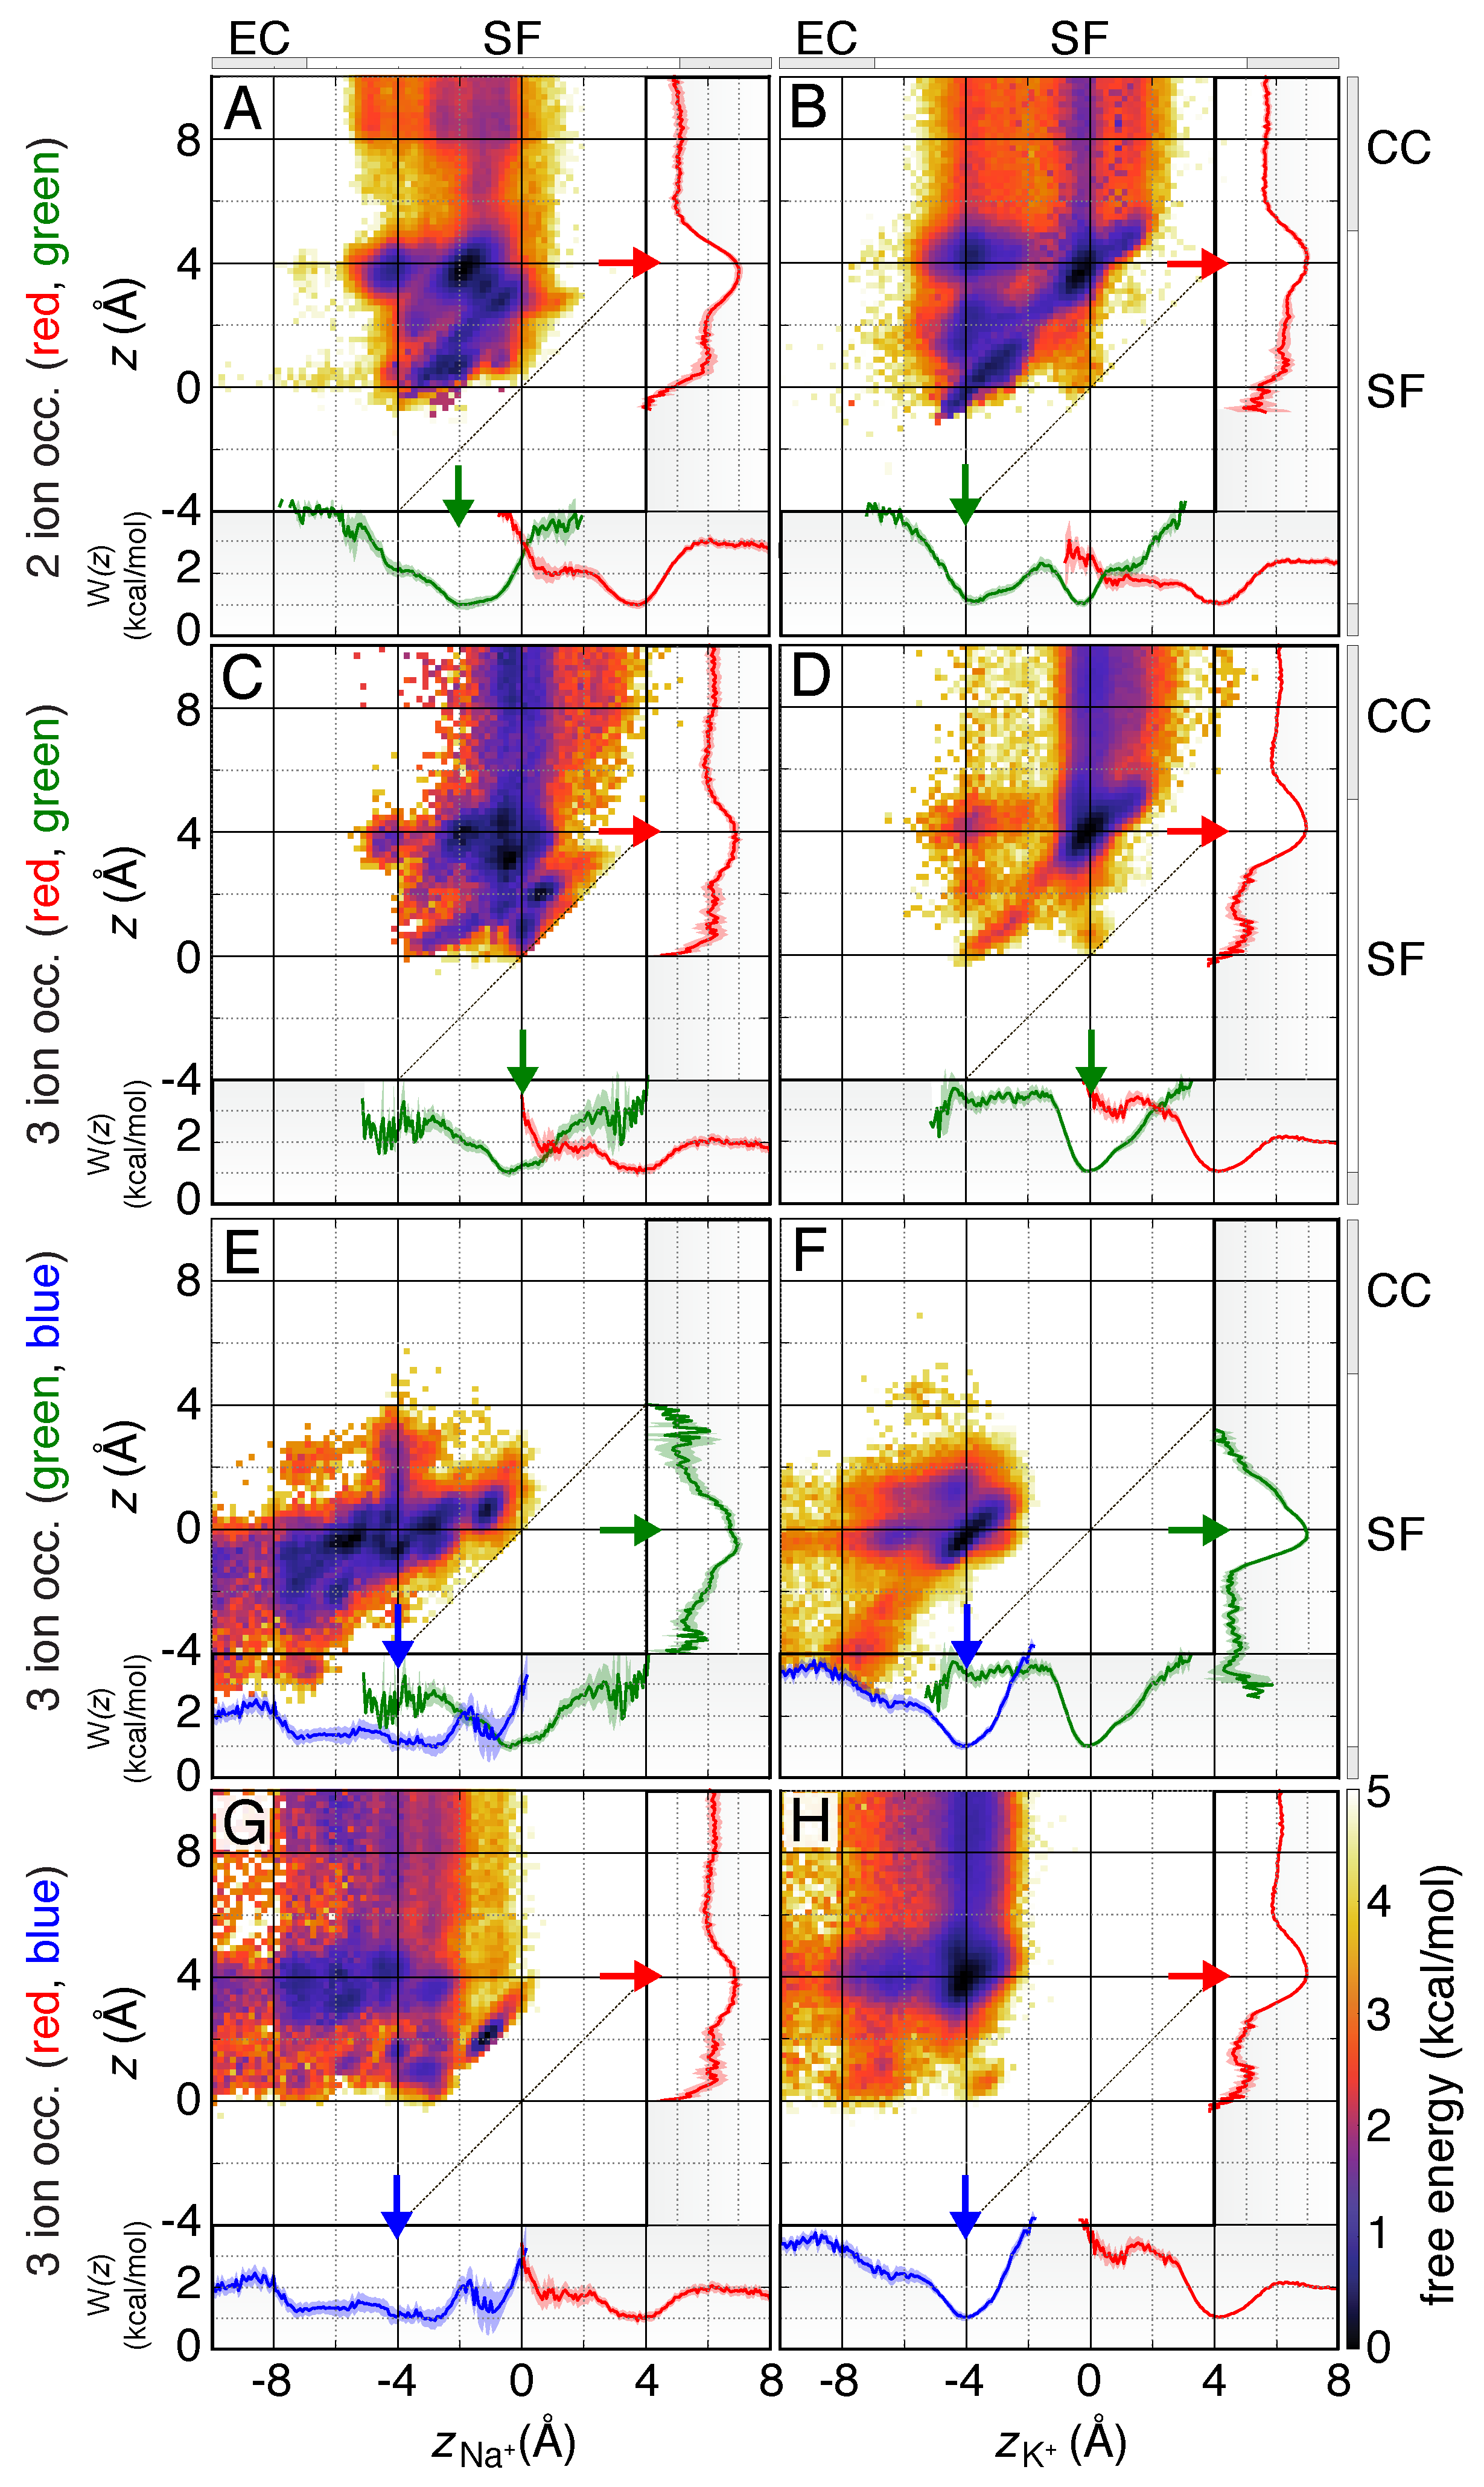
\includegraphics[width=0.6\textwidth]{nav2/Nav2Fig3}
\caption[Two-dimensional potential of mean-force (PMF) for Na$^+$ and K$^+$ pairs along the channel axis]{\textbf{Two-dimensional potential of mean-force (PMF) for Na$^+$ and K$^+$ pairs along the channel axis}. (\textbf{A}) Free energy landscape for (left) Na$^+$ and (right) K$^+$ pairs in the PD+VSD model. Ions are ranked by axial position from CC to EC with the colors `red', `green', and `blue' for both ion types. PMFs for Na$^+$ and K$^+$ are computed between ion pairs for channel occupancy states; (A, B) 2 and (C-H) 3. The populations of 2 and 3 ion states are 767 and 238\% for Na$^+$, respectively. For K$^+$, the populations are 488 and 518\% for 2 and 3 states respectively. One-dimensional projections of the axial free energy for each ion are shown on the vertical and horizontal axes and are colored for the target ion (identified with colored arrows). The reference state (zero free energy) of each panel is set to the highest probability microstate within each channel occupancy state sub-ensemble, which applies to all subsequent ion pair 2D PMFs.}
\label{fig:nav2fig3}
\end{figure}

The presence of a liquid-like free energy landscape for Na$^+$ is even more apparent in the 3 ion occupancy state (Fig. \ref{fig:nav2fig3} C-H). In both the 2 and 3 ion occupancy states, the innermost ion (red) occupies the same lowest free energy state at `LT' for Na$^+$ and K$^+$ (Fig. \ref{fig:nav2fig3} C-D). However, the `LT' to `CC' free energy barrier height is lower in the 3 ion state for Na$^+$ compared to the 2 ion state. A green Na$^+$ samples a broad basin from -3 to 3 \AA, whereas a green K$^+$ collapses to only the `EL' binding site (where the `E' is occupied by the blue ion). Low free energy is observed directly along the diagonal, indicating that both red and green Na$^+$ frequently sample the same axial position at 0 \AA, specifically in the 3 ion occupancy state (Fig. \ref{fig:nav2fig3} C). The free energy basin for the blue Na$^+$ is broader than that of the green Na$^+$ in the 2 ion occupancy state, sampling a series of distinct microstates along the entire -10 to 0 \AA \, range, nearly all of which permit the exit of the red ion (Fig. \ref{fig:nav2fig3} G). The blue K$^+$ ion samples a single minimum at the `E' binding site and also permits the exit of the red ion at this position (Fig. \ref{fig:nav2fig3} H). Overall, these results demonstrate that Na$^+$ moves along a diffusive energy landscape most pronounced in the 3 ion occupancy state, but that K$^+$ is restricted to distinct single-file arrangements.

Previous studies have described the permeation of Na$^+$ as proceeding though a loosely coupled knock-on mechanism \cite{Ing:2016em}. Here we describe this process within the context of our 2D PMF and compare this to K$^+$. Low free energy pathways parallel to the diagonal indicates that concerted motion of red and green ions is possible for both Na$^+$ and K$^+$, and corresponds to the lowest free energy pathway for both ions in the 2 ion state (Fig. \ref{fig:nav2fig3} A-B). In the 3 ion state, concerted motion of the red/green and blue/green pairs are also possible for Na$^+$, forming overlapping energy surfaces and spanning a large range of the SF (Fig. \ref{fig:nav2fig3} C,E). By contrast, concerted motion of red/green and blue/green pairs are seen for K$^+$, but are largely restricted to the confines of the `E', `EL', and `LT' binding sites (Fig. \ref{fig:nav2fig3} D,F). These pairwise free energy surfaces are non-overlapping, and thus give rise to a free energy barrier between the `E' and `EL' sites. Alternatively, a step-wise knock-on mechanism, characterized by a low free energy pathway involving independent movement of the green and red ions, is also possible for both Na$^+$ and K$^+$, but which is higher in free energy for K$^+$ in the 2 ion state as a result of the `E' to `EL' barrier for the green ion (Fig. \ref{fig:nav2fig3} A-B). Based on lowest free energy pathways in the 2 ion state, the movement of ions through the SF is diffusive for Na$^+$, but more rugged for K$^+$. In the 3 ion state, step-wise knock-on is evident from the blue-red ion distributions, showing low free energy pathways for the entrance of the blue ion to a position in the range -6 to -2 \AA, followed by exit of the red ion. In both concerted and step-wise knock-on, we refer to the process of Na$^+$ conduction as loose because the presence of the outermost ion (blue) modifies the free energy landscape, and that ions can exchange position within the SF. This process is facilitated by the movement of Glu side chains, and therefore the multi-ion occupancy of the SF by a variable number of channel groups, results in liquid-like ionic motion in the SF. This mechanism was investigated in our previous study and is qualitatively confirmed here. The mechanism for K$^+$ permeation essentially obeys a single-file knock-on, where ions move in a concerted way when they occupy two of the three binding sites within the SF. In particular, the green ion is capable of adopting the `E' or `EL' binding site depending on the channel occupancy. 

1D projections of the free energy of ionic movement for distinct ions, ranked `red', `green', and `blue' from extracellular to intracellular, are shown on the side axes of each 2D potential of mean force of each ionic occupancy state (Fig. \ref{fig:nav2fig3}). These projections are reported for 2 and 3 ion states for Na$^+$ and K$^+$ (Fig. \ref{fig:nav2fig3-5} B,D,F,H), with additional detail regarding the binding modes of ions at all preferred binding sites along the pore axis (Fig. \ref{fig:nav2fig3-5} A,C,E,G). The SF of Na\textsubscript{V}Ab supports multiple binding sites and modes for Na$^+$ in both the 2 and 3 ion states, with an even broader and diffusive landscape in the 3 ion state \ref{fig:nav2fig3-5} B,F). By contrast, the binding sites and modes for K$^+$ are relatively unchanged in the 2 and 3 ion occupancy states, with increased occupancy resulting a rigidly defined binding sites \ref{fig:nav2fig3-5} D,H).  

\begin{figure}[!htb]
\centering
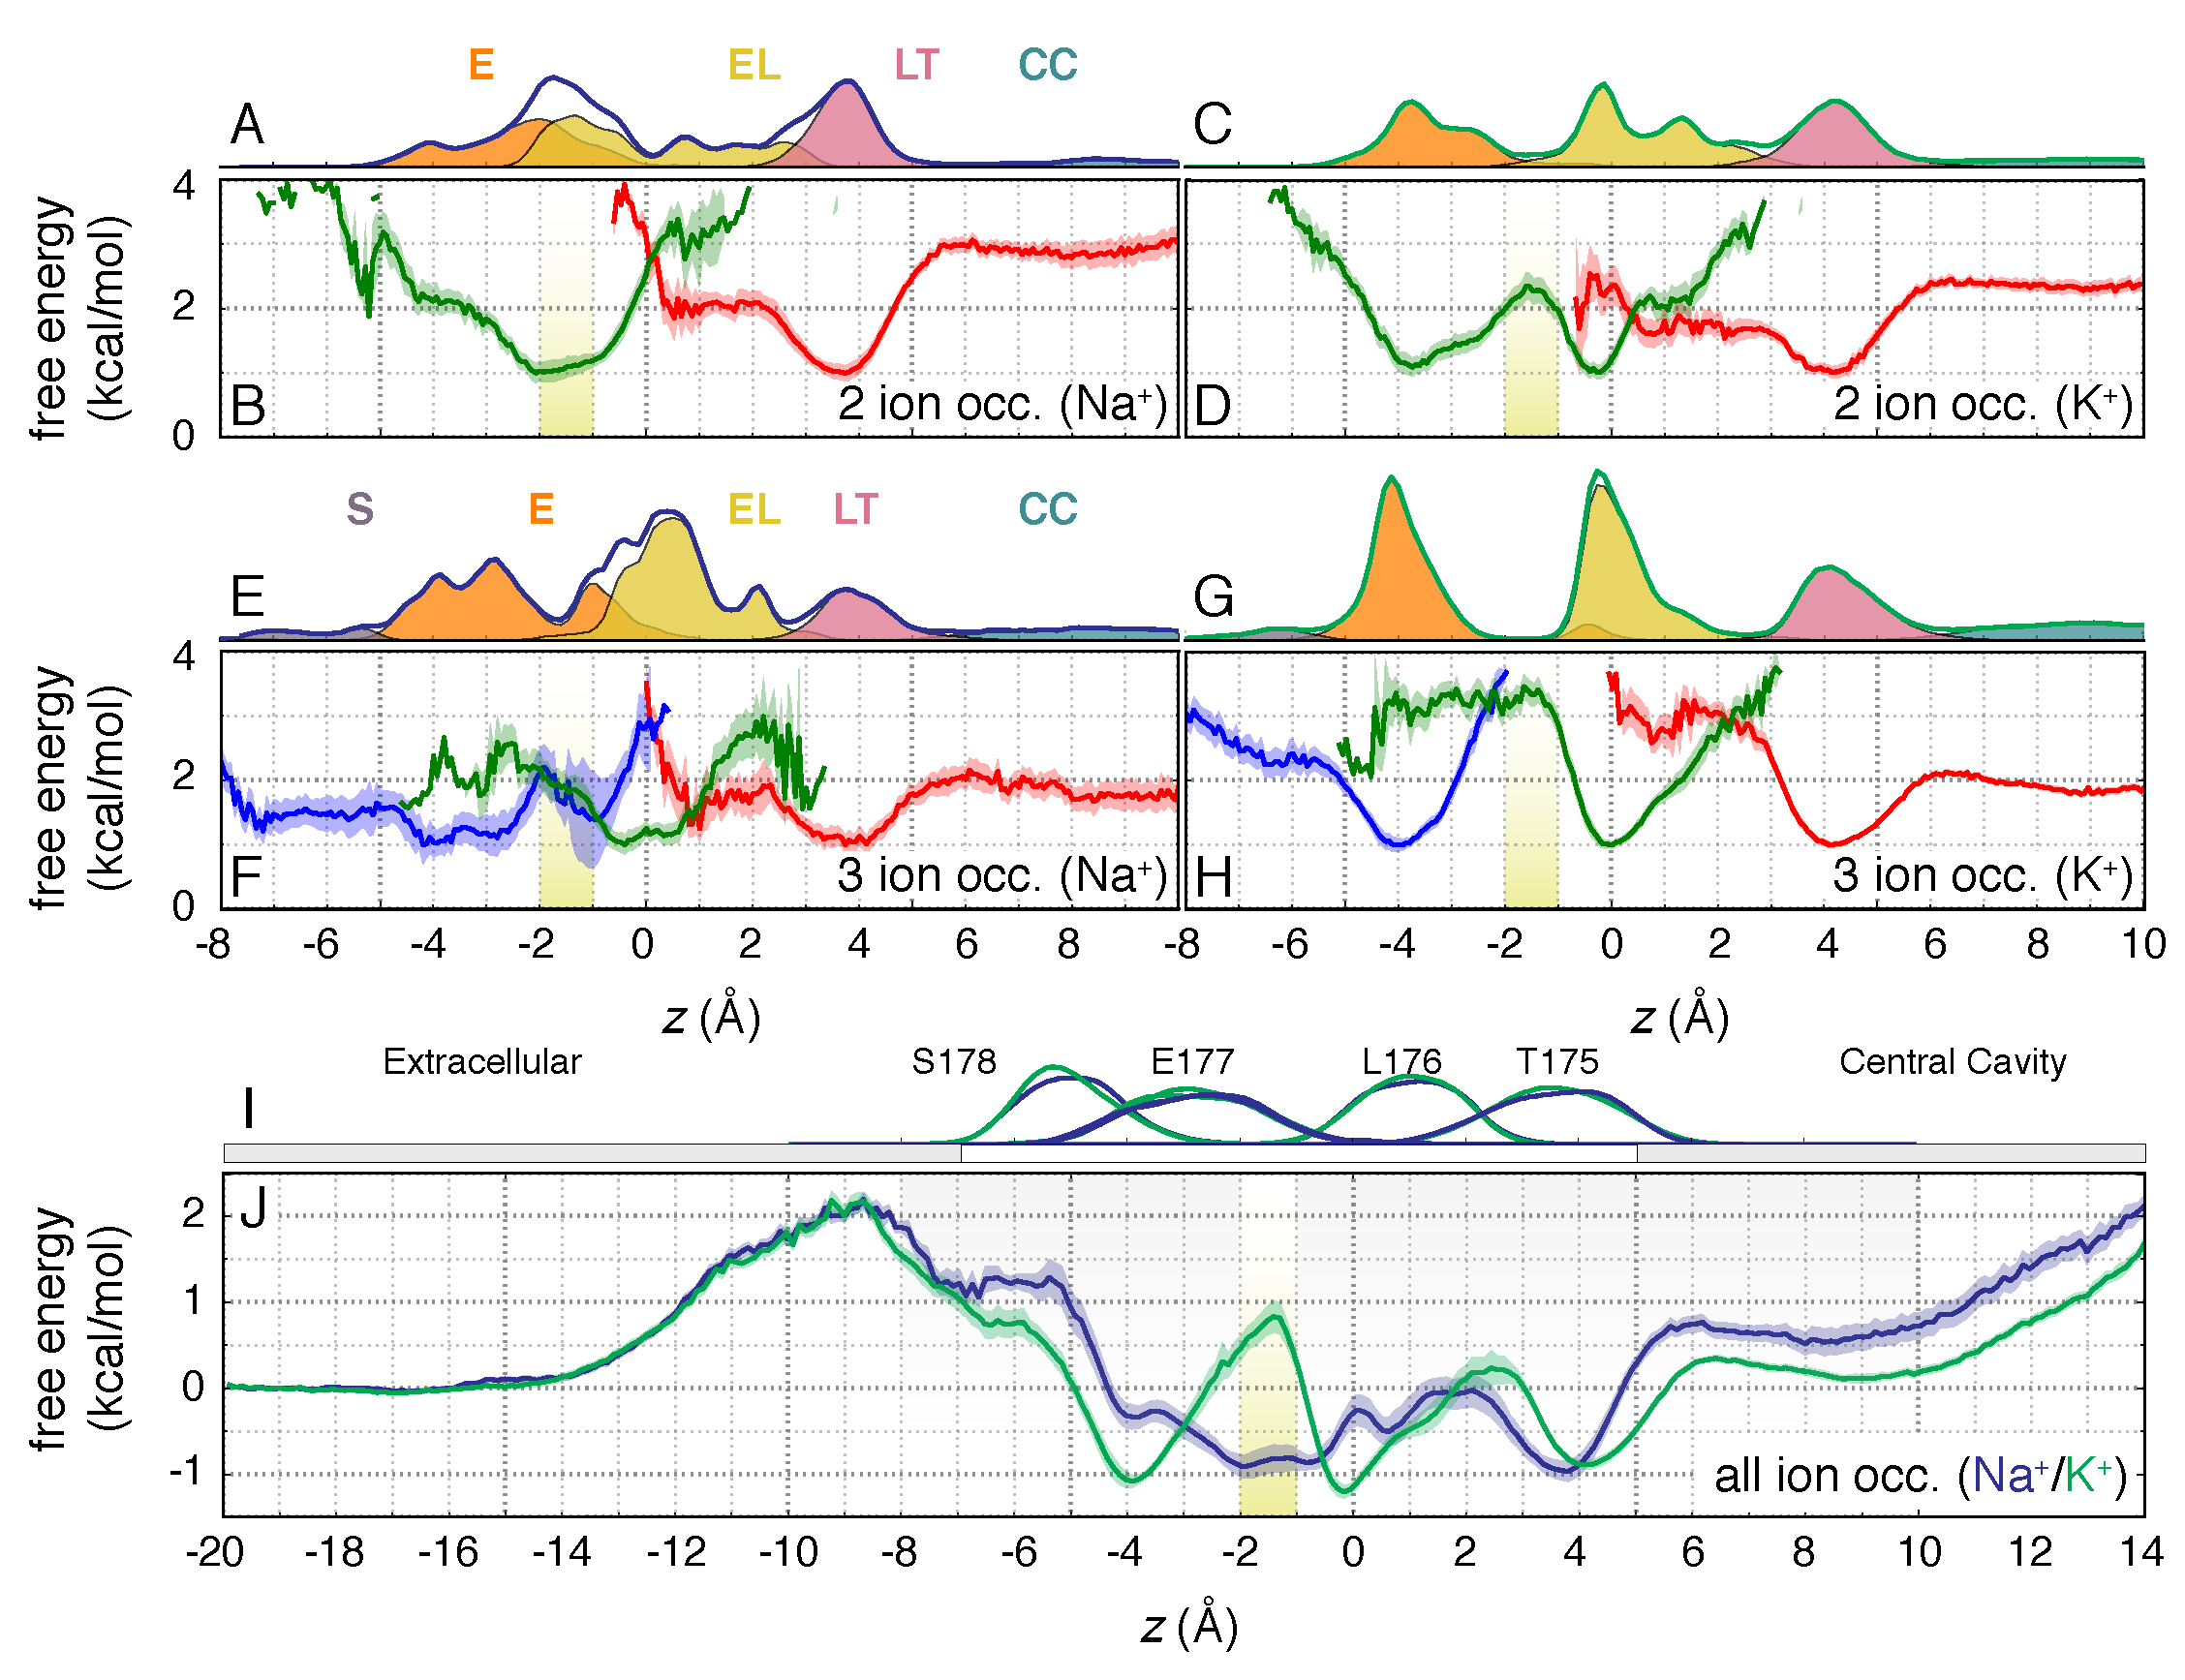
\includegraphics[width=0.6\textwidth]{nav2/Nav2Fig3-5}
\caption[One-dimensional projection of the multi-ion potential of mean-force (PMF) for the movement of Na$^+$ and K$^+$ along the channel axis in distinct occupancy states]{\textbf{One-dimensional projection of the multi-ion potential of mean-force (PMF) for the movement of Na$^+$ and K$^+$ along the channel axis in distinct occupancy states}. (\textbf{A, C}) Distribution of Na$^+$ or K$^+$ along the pore axis for two ion occupancy of the SF, with colored sub-distributions representing the coordination groups of a permeating ion at that axial position. One-dimensional PMFs for (\textbf{B}) Na$^+$ and (\textbf{D}) K$^+$ movement along the channel axis. Ions are ranked by axial position from CC to EC with the colors `red', and `green' for both ion types. (\textbf{E, G}) Distribution of Na$^+$ or K$^+$ along the pore axis for three ion occupancy of the SF with identical coloring to panels (A, C). One-dimensional PMFs for (\textbf{F}) Na$^+$ and (\textbf{G}) K$^+$ movement along the channel axis. Ions are ranked by axial position from CC to EC with the colors `red', `green', and `blue' for both ion types. (\textbf{I}) Axial distribution of channel oxygen atoms, for both Na$^+$ (blue) and K$^+$ (green) simulations. (\textbf{J}) One-dimensional multi-ion PMFs for ionic movement of Na$^+$ (blue) and K$^+$ (green) extended into the extracellular bulk region (set as the free-energy reference state).}
\label{fig:nav2fig3-5}
\end{figure}

The free-energy barrier for K$^+$ conduction in the 2 ion occupancy state, identified in the 2D PMF surfaces (Fig. \ref{fig:nav2fig3} B,D,F), is qualitatively visible in the 1D projection of the free-energy profile using the positions of all Na$^+$ or K$^+$ cations, respectively (Fig. \ref{fig:nav2fig3-5} J). Na$^+$ moves relatively unimpeded (<1 kcal/mol barriers) through the SF whereas a $\sim$1.5-2 kcal/mol barrier separates the `E' and `EL' binding sites for K$^+$ (identified throughout the manuscript with a gold shaded region, Fig. \ref{fig:nav2fig3-5} J). Note that these pseudo-PMFs obscure the true height of the free energy barriers due to the overlap of both two and three ion states, as well as the multi-ion occupancy of certain free energy basins, but can be used as a short-hand signature of the actual free energy landscape. 

2D PMFs indicate that the ionic occupancy modifies the free energy surface for the innermost red ion, promoting ion translocation into the `CC' the 3 ion state. However, we do not make the assumption that an ion in the central cavity is a valid description of the fully translocated ion (see Discussion), but focus on the entry and exit of ions in and out of the SF. The fluxes between the 2 and 3 occupancy states are computed for Na$^+$ and K$^+$ in both the PD+VSD and PD models (Fig. \ref{fig:nav2figS8}). The forward and backward flux between these occupancy macrostates are roughly equivalent, suggesting that ion rearrangement within the SF are near equilibrium on the timescale of our simulations. In pure cation simulations, K$^+$ exchanges between 2 and 3 ion states twice as fast as Na$^+$, but this exchange is on the same order of magnitude in mixed cation simulations.

\begin{figure}[!htb]
\centering
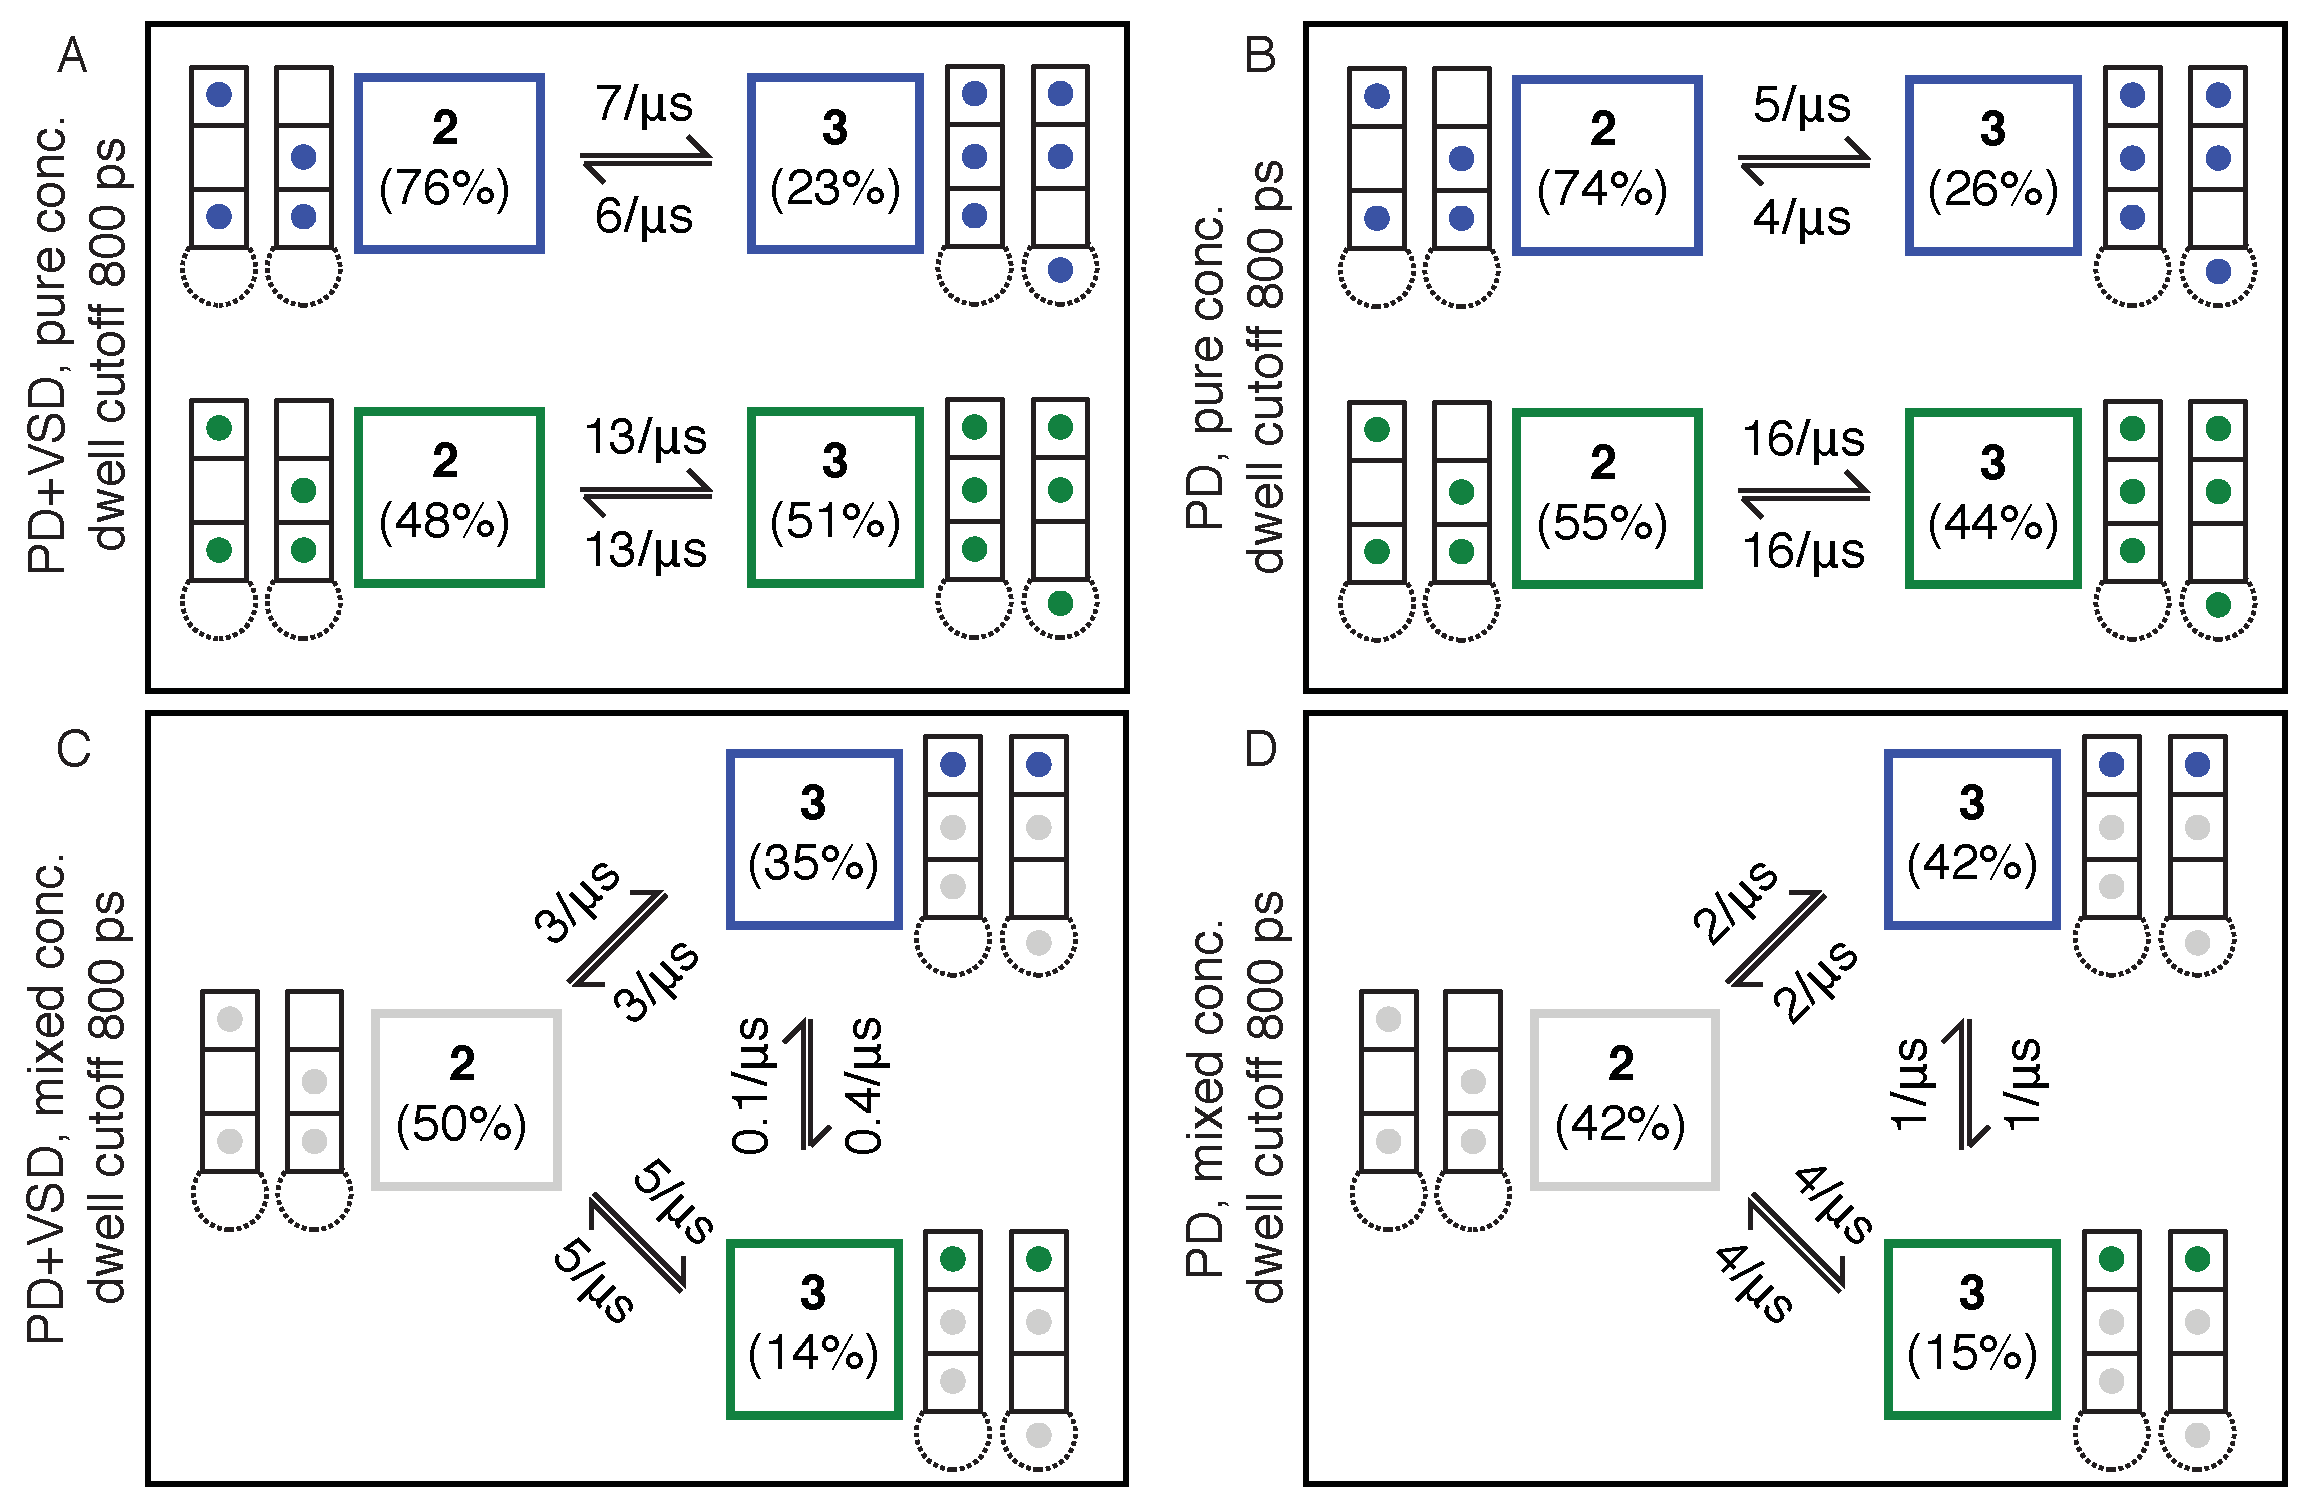
\includegraphics[width=0.6\textwidth]{nav2/Nav2FigS8}
\caption[Occupancy Macrostate Kinetics of Na$^+$ and K$^+$]{\textbf{Occupancy Macrostate Kinetics of Na$^+$ and K$^+$}. Square boxes (blue for Na$^+$, green for K$^+$) represent the primary channel macrostates, 2 and 3, with macrostate populations are shown within each box. Bidirectional arrows between macrostates indicate the average ionic flux between two states across all replicas. Kinetic diagram illustrating ion flux into the SF for pure cation concentrations in the (\textbf{A}) PD+VSD and (\textbf{B}) PD models and ion flux into the SF from mixed cation simulations in the (\textbf{C}) PD+VSD and (\textbf{D}) PD models. In mixed cation simulations, we distinguish between entry of Na$^+$ and K$^+$ to form the 3 ion occupancy state. Transitions between states failing to start and end in a macrostate for a dwell time of 800 ps are removed from this analysis, reducing over-counting of fast transitions.}
\label{fig:nav2figS8}
\end{figure}

\subsection{Mixed Cations in the Na\textsubscript{V}Ab Pore}

\begin{figure}[!htb]
\centering
\includegraphics[width=0.7\textwidth]{nav2/Nav2FigS2}
\caption[Sodium and potassium ion movement in the selectivity filter of Na\textsubscript{V}Ab from a mixed concentration simulations in the PD+VSD model]{\textbf{Sodium and potassium ion movement in the selectivity filter of Na\textsubscript{V}Ab from a mixed concentration simulations in the PD+VSD model}. (\textbf{A}) Representative snapshots of Na$^+$ (blue spheres) and K$^+$ ions (green spheres) in the SF are shown at specified time steps. The pore-lining oxygen groups of the SF (backbone carbonyl groups of T175 and L176 and the side chains of E177 and S178) are shown. (\textbf{B, D}) Dynamics of Na$^+$ and K$^+$ ions along the pore axis from different simulation repeats. Colored bars at the bottom of each time series indicate the channel occupancy (legend in top right). Distribution of (\textbf{C}) Na$^+$ or (\textbf{E}) K$^+$ cations along the pore axis over all simulation repeats, with colored sub-distributions indicating which of the SF residues T, L, E, S coordinate a permeating ion at that axial position. Distributions are normalized by channel average channel occupancy of each ion type. }
\label{fig:nav2figS2}
\end{figure}

%In addition, electrophysiological measurements of Na\textsubscript{V}Ab were performed successively in pure cation and bi-ionic conditions (Fig. \ref{fig:nav2figS11}). Relative permeabilities computed using either the ratio of normalized peak conductance or the reversal potential confirm that Na\textsubscript{V}Ab is permeable to cations in mixed cation concentrations, in agreement with the measured selectivity of bacterial channel NaChBac \cite{FinolUrdaneta:2014bz}.

We studied competitive binding of Na$^+$ and K$^+$ in the SF using MD simulations in presence of mixed NaCl and KCl solutions. Four selected time trajectories of mixed NaCl and KCl solutions in the PD+VSD model reveal a diverse number of ionic arrangements within the SF (Fig.  \ref{fig:nav2figS2}). Na$^+$ and K$^+$ may occupy the same axial position in the `EL' binding site, permitting exchanges of these ions within the SF (Fig. \ref{fig:nav2figS2} A iv, v). Average axial distributions of Na$^+$ and K$^+$ across all simulation repeats show that all the binding sites found in pure cation simulations are occupied (Fig. \ref{fig:nav2figS2} C,E). A projected free energy barrier separating the `E' and `EL' sites is still seen in the multi-ion PMF for K$^+$ in mixed cation simulations (Fig. \ref{fig:nav2fig4} C). Although the relative binding affinities of the `E', `EL', and `LT' sites are unchanged for Na$^+$ and K$^+$ (Fig. \ref{fig:nav2fig4} C), there is a difference in occupancy of these sites. Overall, ion occupancy of the pore is mixed 66\% of the time, whereas Na$^+$-only and K$^+$-only occupancy are observed 34 and 0\% of the time, respectively (see the most populated channel configurations in Fig. \ref{fig:nav2fig4} H). Cation competition has dramatic effects on relative binding propensities in the SF. In pure-cation simulations, the SF is occupied by $2.0 \pm 0.1$ cations for both Na$^+$ and K$^+$ (Fig. \ref{fig:nav2fig2} B), but the SF becomes 25\% more Na$^+$ selective when the two cations are competing ($1.21 \pm 0.04$ vs. $0.97 \pm 0.04$, for Na$^+$ and K$^+$, respectively, Fig. \ref{fig:nav2fig4} G). Binding occupancies of the competing ions show 86\% and 20\% preferences for Na$^+$ over K$^+$ in the `E' and `EL' sites, respectively, corresponding to a free energy difference of $\sim 0.5$kT at 300 K. Even though Na$^+$ and K$^+$ do not share a binding site in the highest population ionic configurations within the channel (Fig. \ref{fig:nav2fig4} H), all-ion pair 2D PMFs show that it is possible for Na$^+$ to pass itself and K$^+$ in mixed cation simulations (Fig. \ref{fig:nav2figS7} C-E).

\begin{figure}[!ptb]
\centering
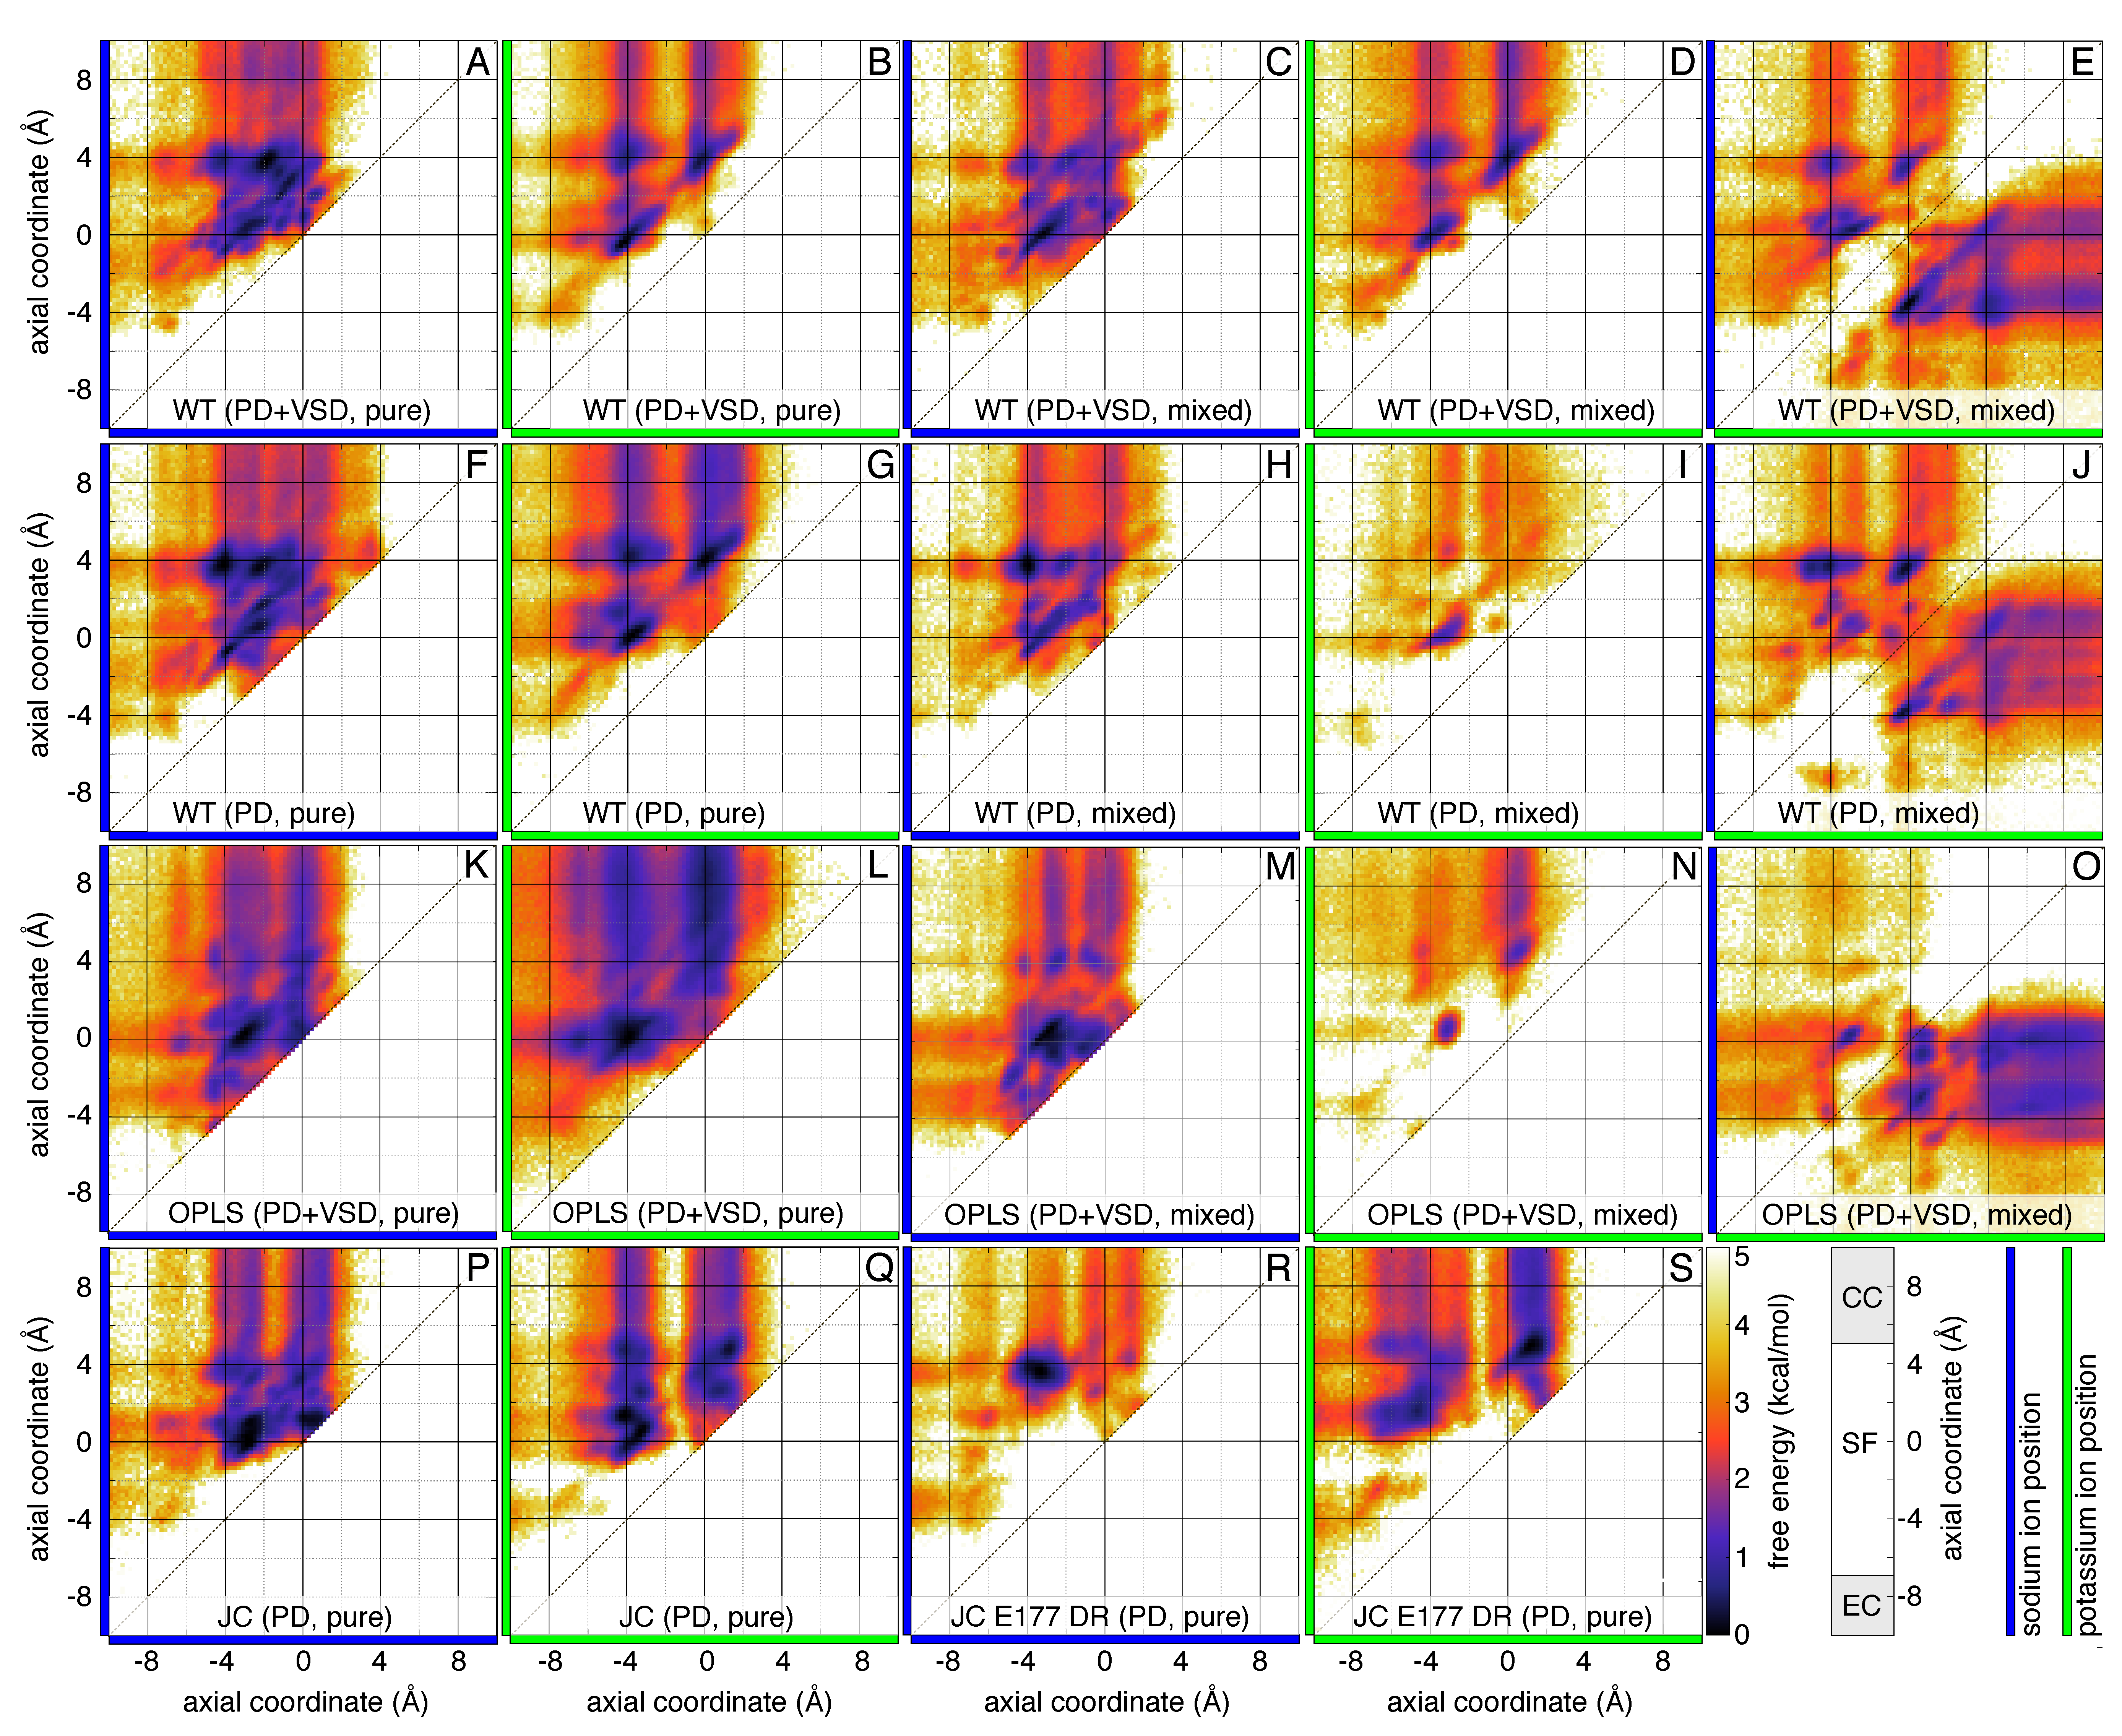
\includegraphics[width=0.7\textwidth]{nav2/Nav2FigS7}
\caption[Two-dimensional potential of mean-force (PMF) for Na$^+$ and K$^+$ pairs along the channel axis]{\textbf{Two-dimensional potential of mean-force (PMF) for Na$^+$ and K$^+$ pairs along the channel axis}. Ionic species are identified by a colored bar on the axes, Na$^+$ (blue) and K$^+$ (green). PMFs for (\textbf{A}) Na$^+$-Na$^+$ and (\textbf{B}) K$^+$-K$^+$ in pure cation simulations, and (\textbf{C-E}) Na$^+$-Na$^+$, K$^+$-K$^+$, and Na$^+$-K$^+$ in mixed cation simulations in the PD+VSD model. (\textbf{F}) Na$^+$-Na$^+$ and (\textbf{G}) K$^+$-K$^+$ in pure cation simulations, and (\textbf{H-J}) Na$^+$-Na$^+$, K$^+$-K$^+$, and Na$^+$-K$^+$ in mixed cation simulations in the PD model. PMFs for the (\textbf{K-O}) OPLS model, (\textbf{P-Q}) JC model, and (\textbf{R-S}) JC model E177 dihedral restraints. The reference state (zero free energy) is set to the high probability state for each pure cation or mixed cation simulation dataset, respectively.}
\label{fig:nav2figS7}
\end{figure}

\begin{figure}[!htb]
\centering
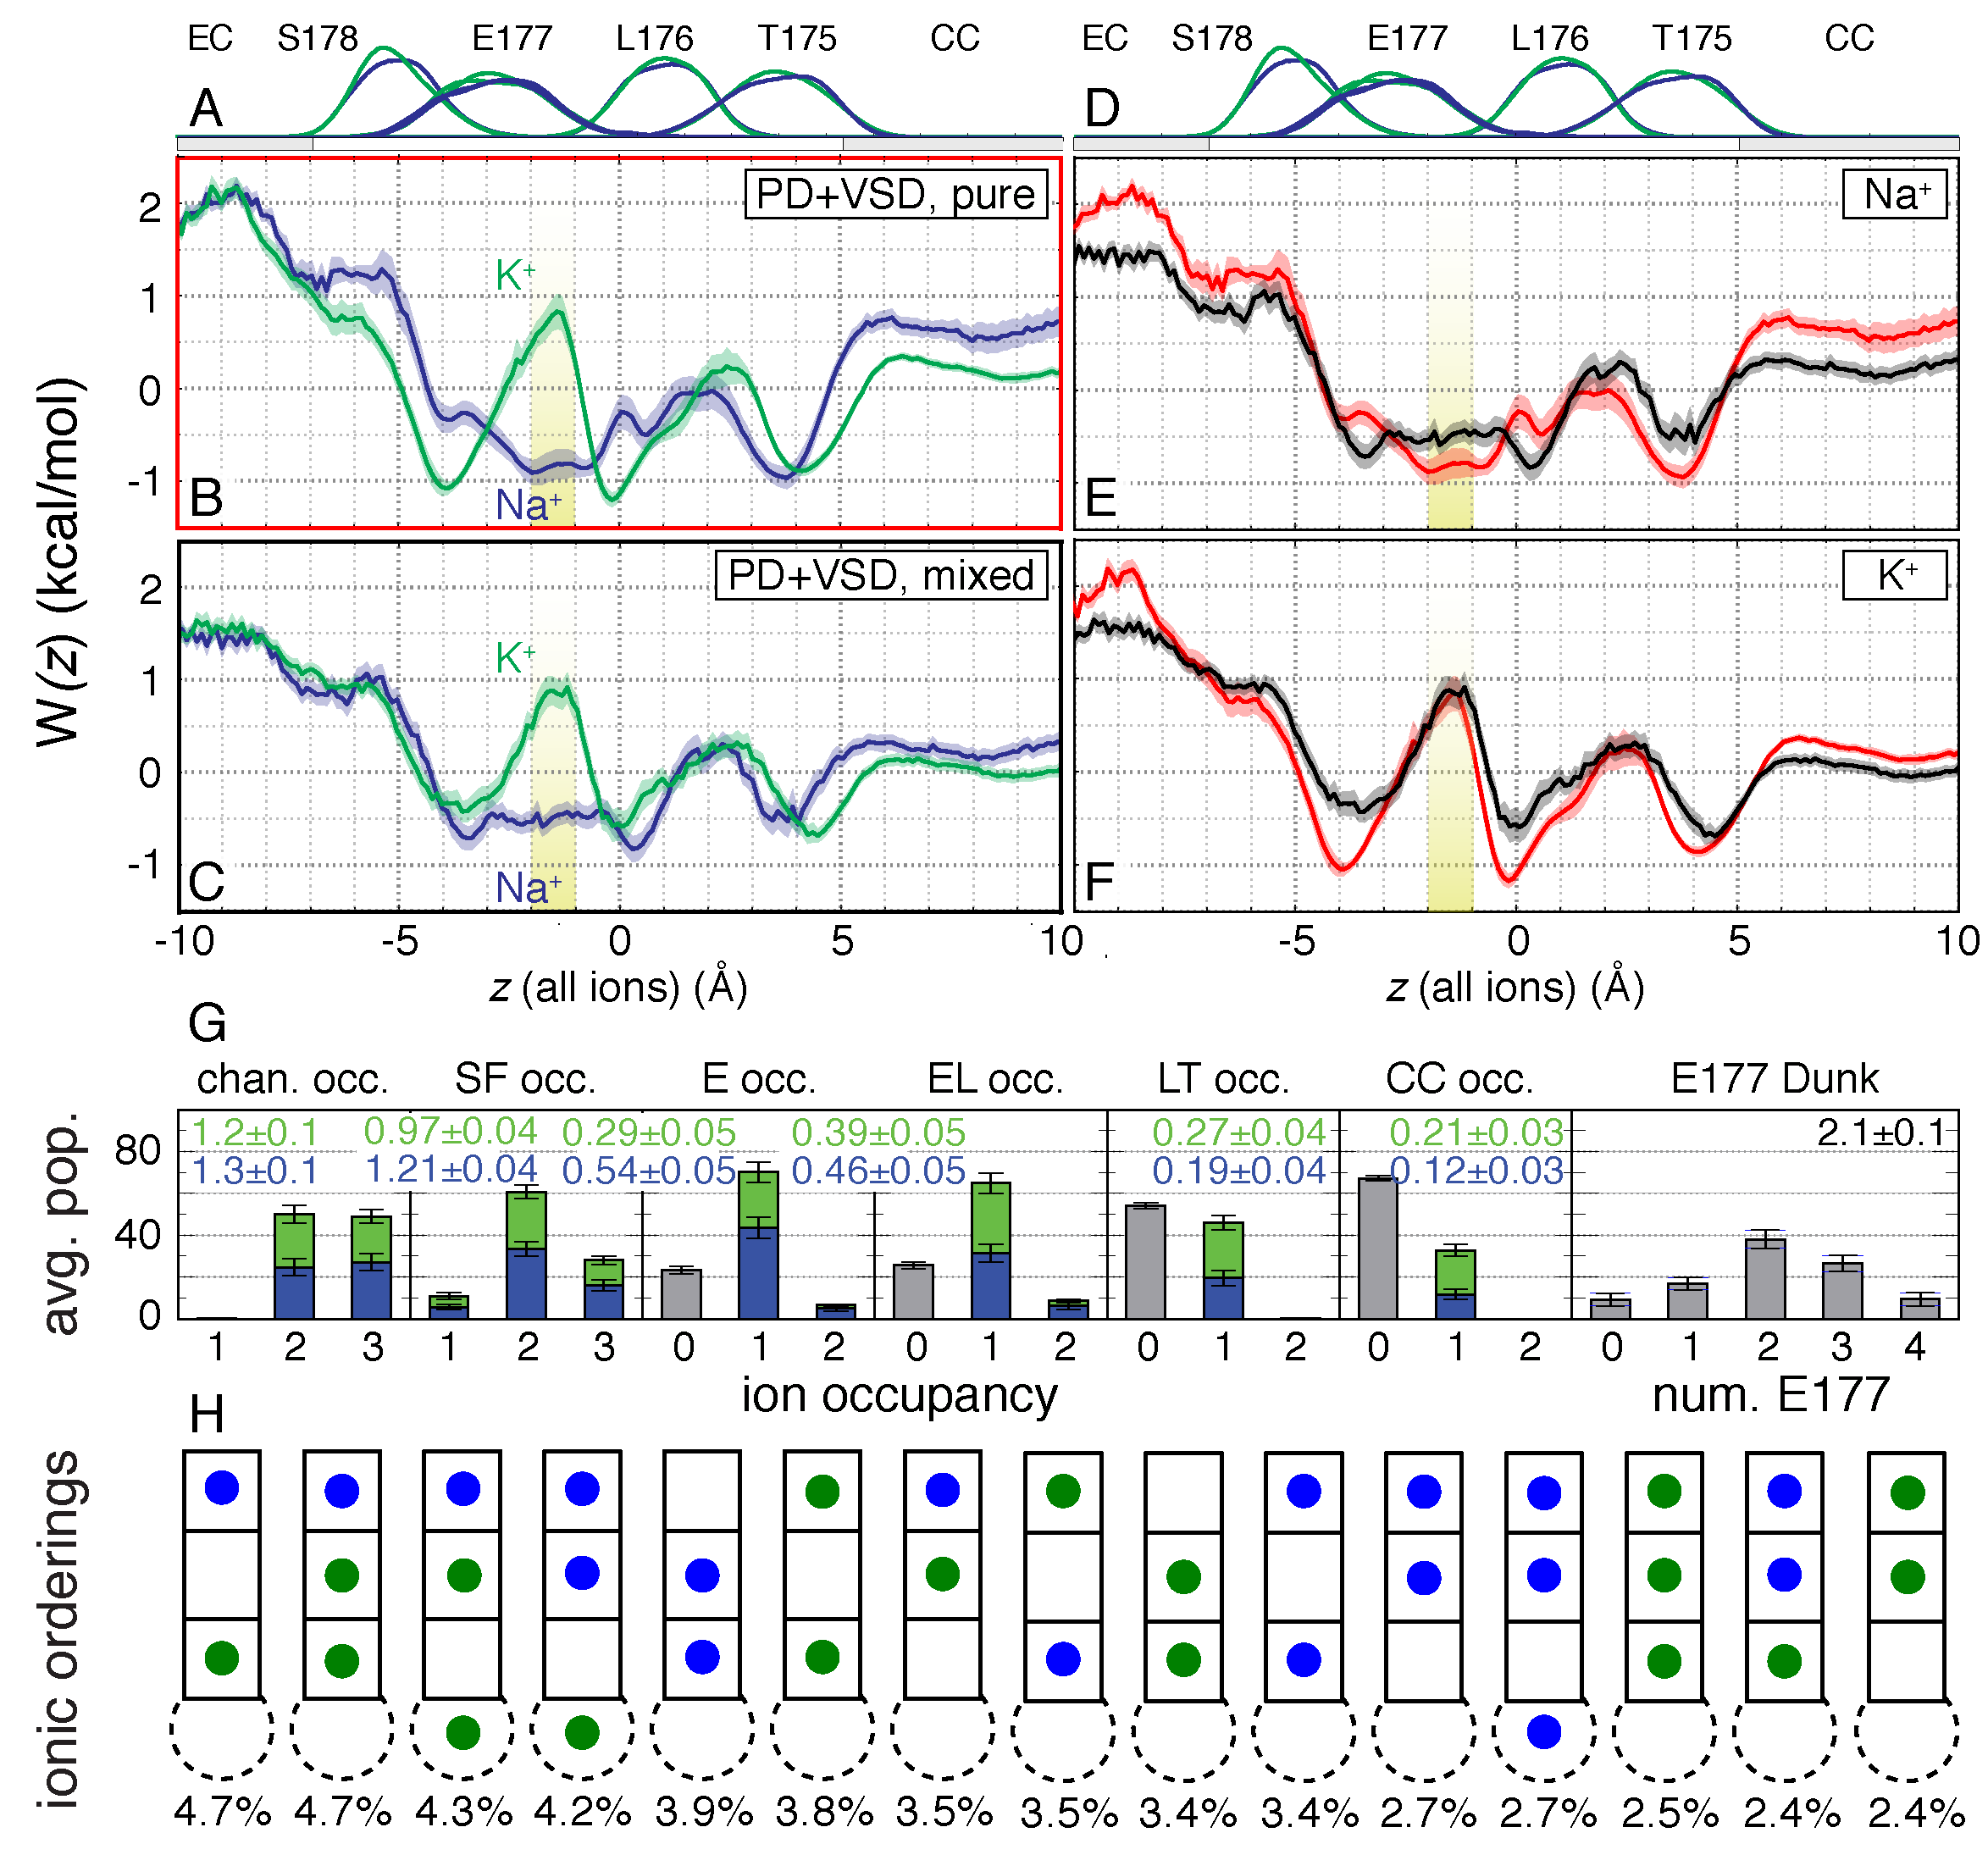
\includegraphics[width=0.6\textwidth]{nav2/Nav2Fig4}
\caption[The effect of competitive binding of Na$^+$ and K$^+$ along the channel axis]{\textbf{The effect of competitive binding of Na$^+$ and K$^+$ along the channel axis}. (\textbf{A,D}) Axial distribution of channel oxygen atoms. One-dimensional multi-ion PMFs for ionic movement of (\textbf{B}) pure Na$^+$ (blue) and K$^+$ (green) and (\textbf{C}) mixed Na$^+$ and K$^+$ along the channel axis in the PD+VSD model. To help comparison between datasets, an overlays of 1D multi-ion PMFs for (\textbf{E}) Na$^+$ and (\textbf{F}) K$^+$ are also shown. The reference state (zero free energy) is defined as the bulk extracellular value of Na$^+$ and K$^+$ separately. A gold band indicates the region of highest free-energy barrier for K$^+$ permeation within the SF. The axial distribution of pore-lining oxygen atoms of T175, L176, E177, and S178 are shown from PD+VSD simulations for Na$^+$ (blue) and K$^+$ (green) above panels (A, D). Ionic occupancy is shown from left to right for the entire channel, the SF, all major binding sites within the SF, together with the number of dunked E177 side chains for (\textbf{F}) mixed cation simulations. (\textbf{G}) Ionic occupancy of binding sites (E, EL, LT, CC) in the highest population channel configurations from mixed cation simulations.}
\label{fig:nav2fig4}
\end{figure}

\subsection{Solvation of Na$^+$ and K$^+$ During Permeation}

\begin{figure}[!ptb]
\centering
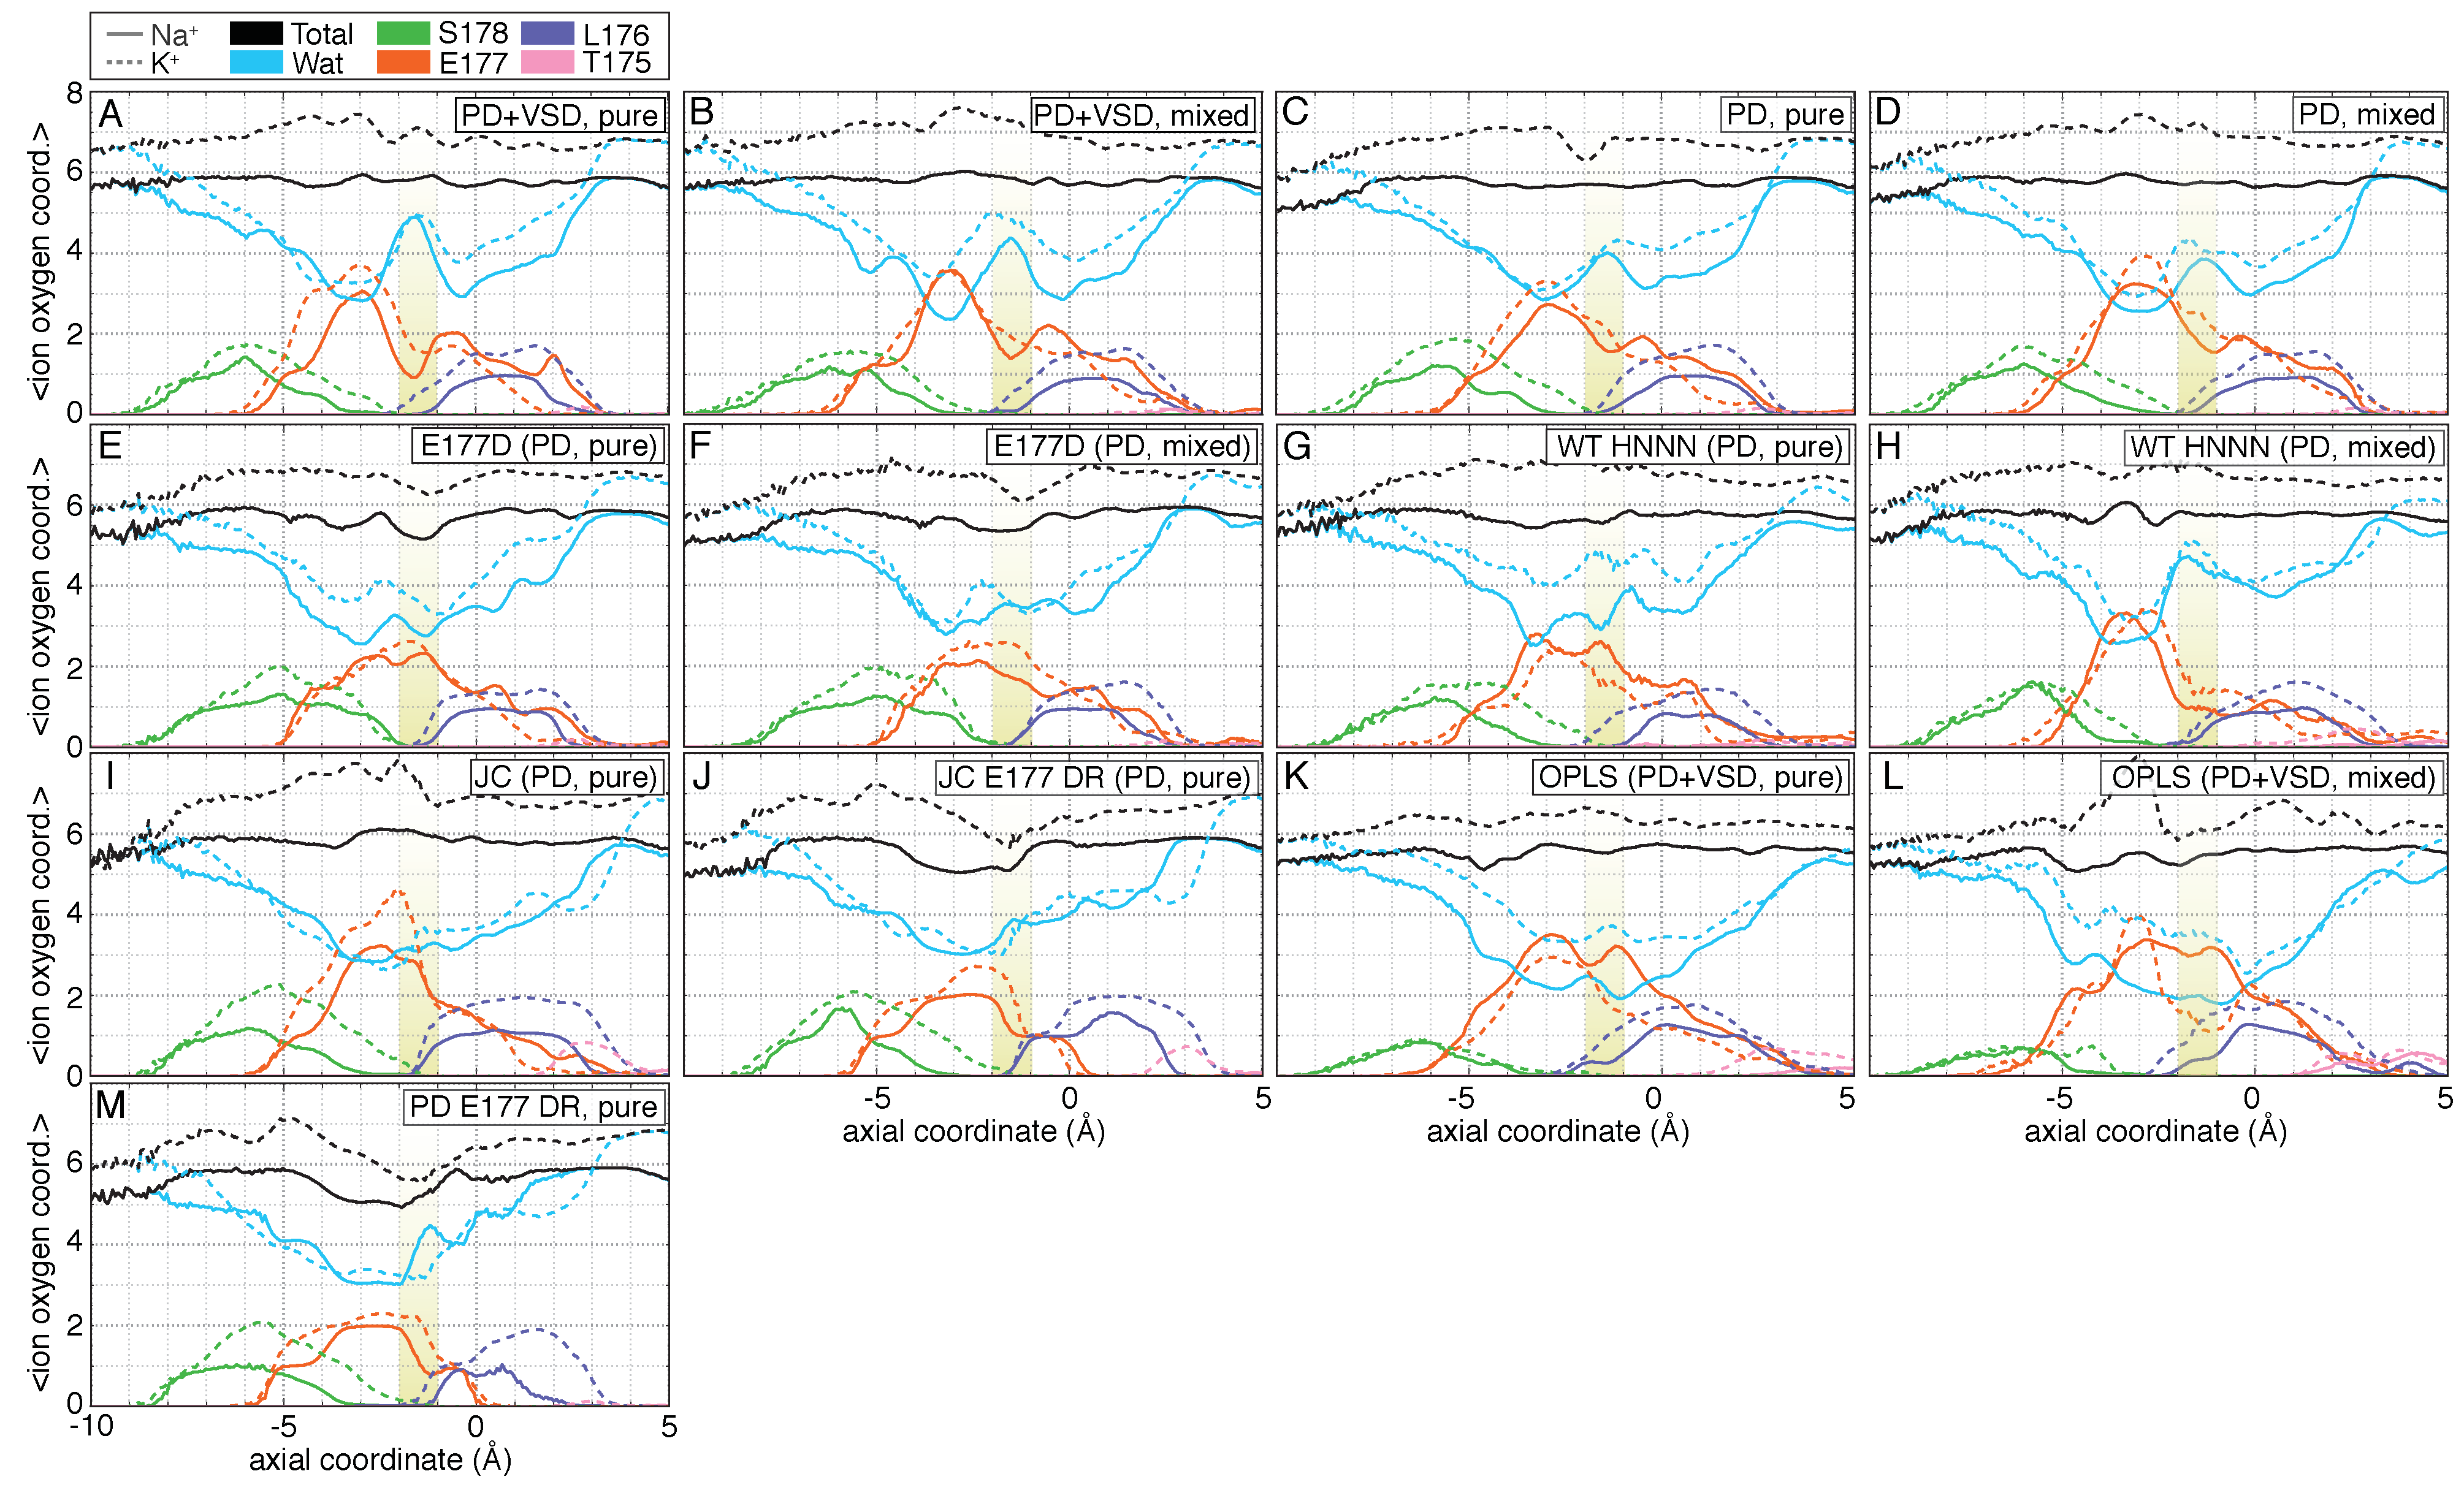
\includegraphics[width=0.9\textwidth]{nav2/Nav2FigS5}
\caption[Average oxygen coordination of Na$^+$ or K$^+$]{\textbf{Average oxygen coordination of Na$^+$ or K$^+$}. The average number of oxygen atoms in the 1st coordination shell of Na$^+$ (solid) and K$^+$ (dashed) as a function of position on the channel axis. Data is shown for the (\textbf{A-B}) PD+VSD model, (\textbf{C-D}) PD model, (\textbf{E-F}) E177D model (where E177 is replaced with D177), (\textbf{G-H}), HNNN model, (\textbf{I-J}) JC model with and without E177 dihedral restraints, the (\textbf{K-L}) OPLS model, and the (\textbf{M}) PD model with E177 dihedral restraints. Individual contributions to the total coordination (black) is depicted for each channel ligand; T175 (pink), L176 (purple), E177 (orange), S178 (green), in addition to water (blue). A gold band indicates the region of highest free-energy barrier for K$^+$ permeation within the SF.}
\label{fig:nav2figS5}
\end{figure}

To examine the basis for preferential binding of Na$^+$ in the SF of Na\textsubscript{V}Ab, we calculate the average coordination of cations by water molecules and channel ligands along the channel axis (Fig. \ref{fig:nav2figS5}).  The average number of O atoms in the first solvation shell varies between 5 and 6 for Na$^+$ and between 6 and 7 for K$^+$, in good quantitative agreement with simulation studies of these two cations in the potassium channel KcsA \cite{Egwolf:2010ki}.  On either side of the SF, the extracellular vestibule or the central cavity, Na$^+$ and K$^+$ are completely hydrated by $5.62\pm0.03$ and $6.51\pm0.02$ water molecules, respectively, and they remain partly hydrated in the SF, where channel coordination is dominated by L176 and E177. Due its larger radius, K$^+$ has marginally higher coordination to channel ligands across the SF than Na$^+$. In the K$^+$ permeation bottleneck, denoted by a gold band, $\sim$1-2 carboxylate O ligands solvate Na$^+$ and K$^+$ together with $\sim$4-5 water molecules, with an additional $\sim$1 carbonyl group for K$^+$ (Fig. \ref{fig:nav2figS5} A). This bottleneck is the position of maximal hydration within the SF for both Na$^+$ and K$^+$ across PD+VSD, PD pure, and PD mixed simulations. Cation solvation is unchanged for Na$^+$ between the pure and mixed cation simulations, but an increase in the number of dunked glutamic acid side chains was observed in mixed cation simulations (Fig. \ref{fig:nav2figS5} A-B). Overall, since solvation is not significantly different for the two cations, and the barrier region corresponds to the maximally hydrated SF position, we conclude that the moderate barrier for K$^+$ at this site is due to the difficulty in hydrating the cation at that location, something which does not occur for Na$^+$. 

\subsection{Effect of conformational isomerization of E177 on cation binding and mobility }

\begin{figure}[!ptb]
\centering
\includegraphics[width=0.7\textwidth]{nav2/Nav2FigS3}
\caption[Sodium and potassium ion movement in the selectivity filter of Na\textsubscript{V}Ab when E177 is restrained in the crystallographic orientation]{\textbf{Sodium and potassium ion movement in the selectivity filter of Na\textsubscript{V}Ab when E177 is restrained in the crystallographic orientation}. (\textbf{A}) Representative snapshots of Na$^+$ (blue spheres) and K$^+$ ions (green spheres) in the SF are shown at specified time steps. The pore-lining oxygen groups of the SF (backbone carbonyl groups of T175 and L176 and the side chains of E177 and S178) are shown. (\textbf{B, D}) Movement of Na$^+$ and K$^+$ ions along the pore axis from different simulation repeats. Colored bars at the bottom of each time series indicate the channel occupancy (legend in top right). (\textbf{C, E}) Distribution of Na$^+$ or K$^+$ along the pore axis over all pure cation simulation repeats, with colored sub-distributions representing the coordination groups of a permeating ion at that axial position. Distributions are normalized by channel average channel occupancy of each ion. (\textbf{F}) Movement of Na$^+$ and K$^+$ ions in a mixed cation simulation with (\textbf{G}) the distribution of Na$^+$ and K$^+$ along the channel axis for all mixed cation simulation repeats.}
\label{fig:nav2figS3}
\end{figure}

\begin{figure}[!htb]
\centering
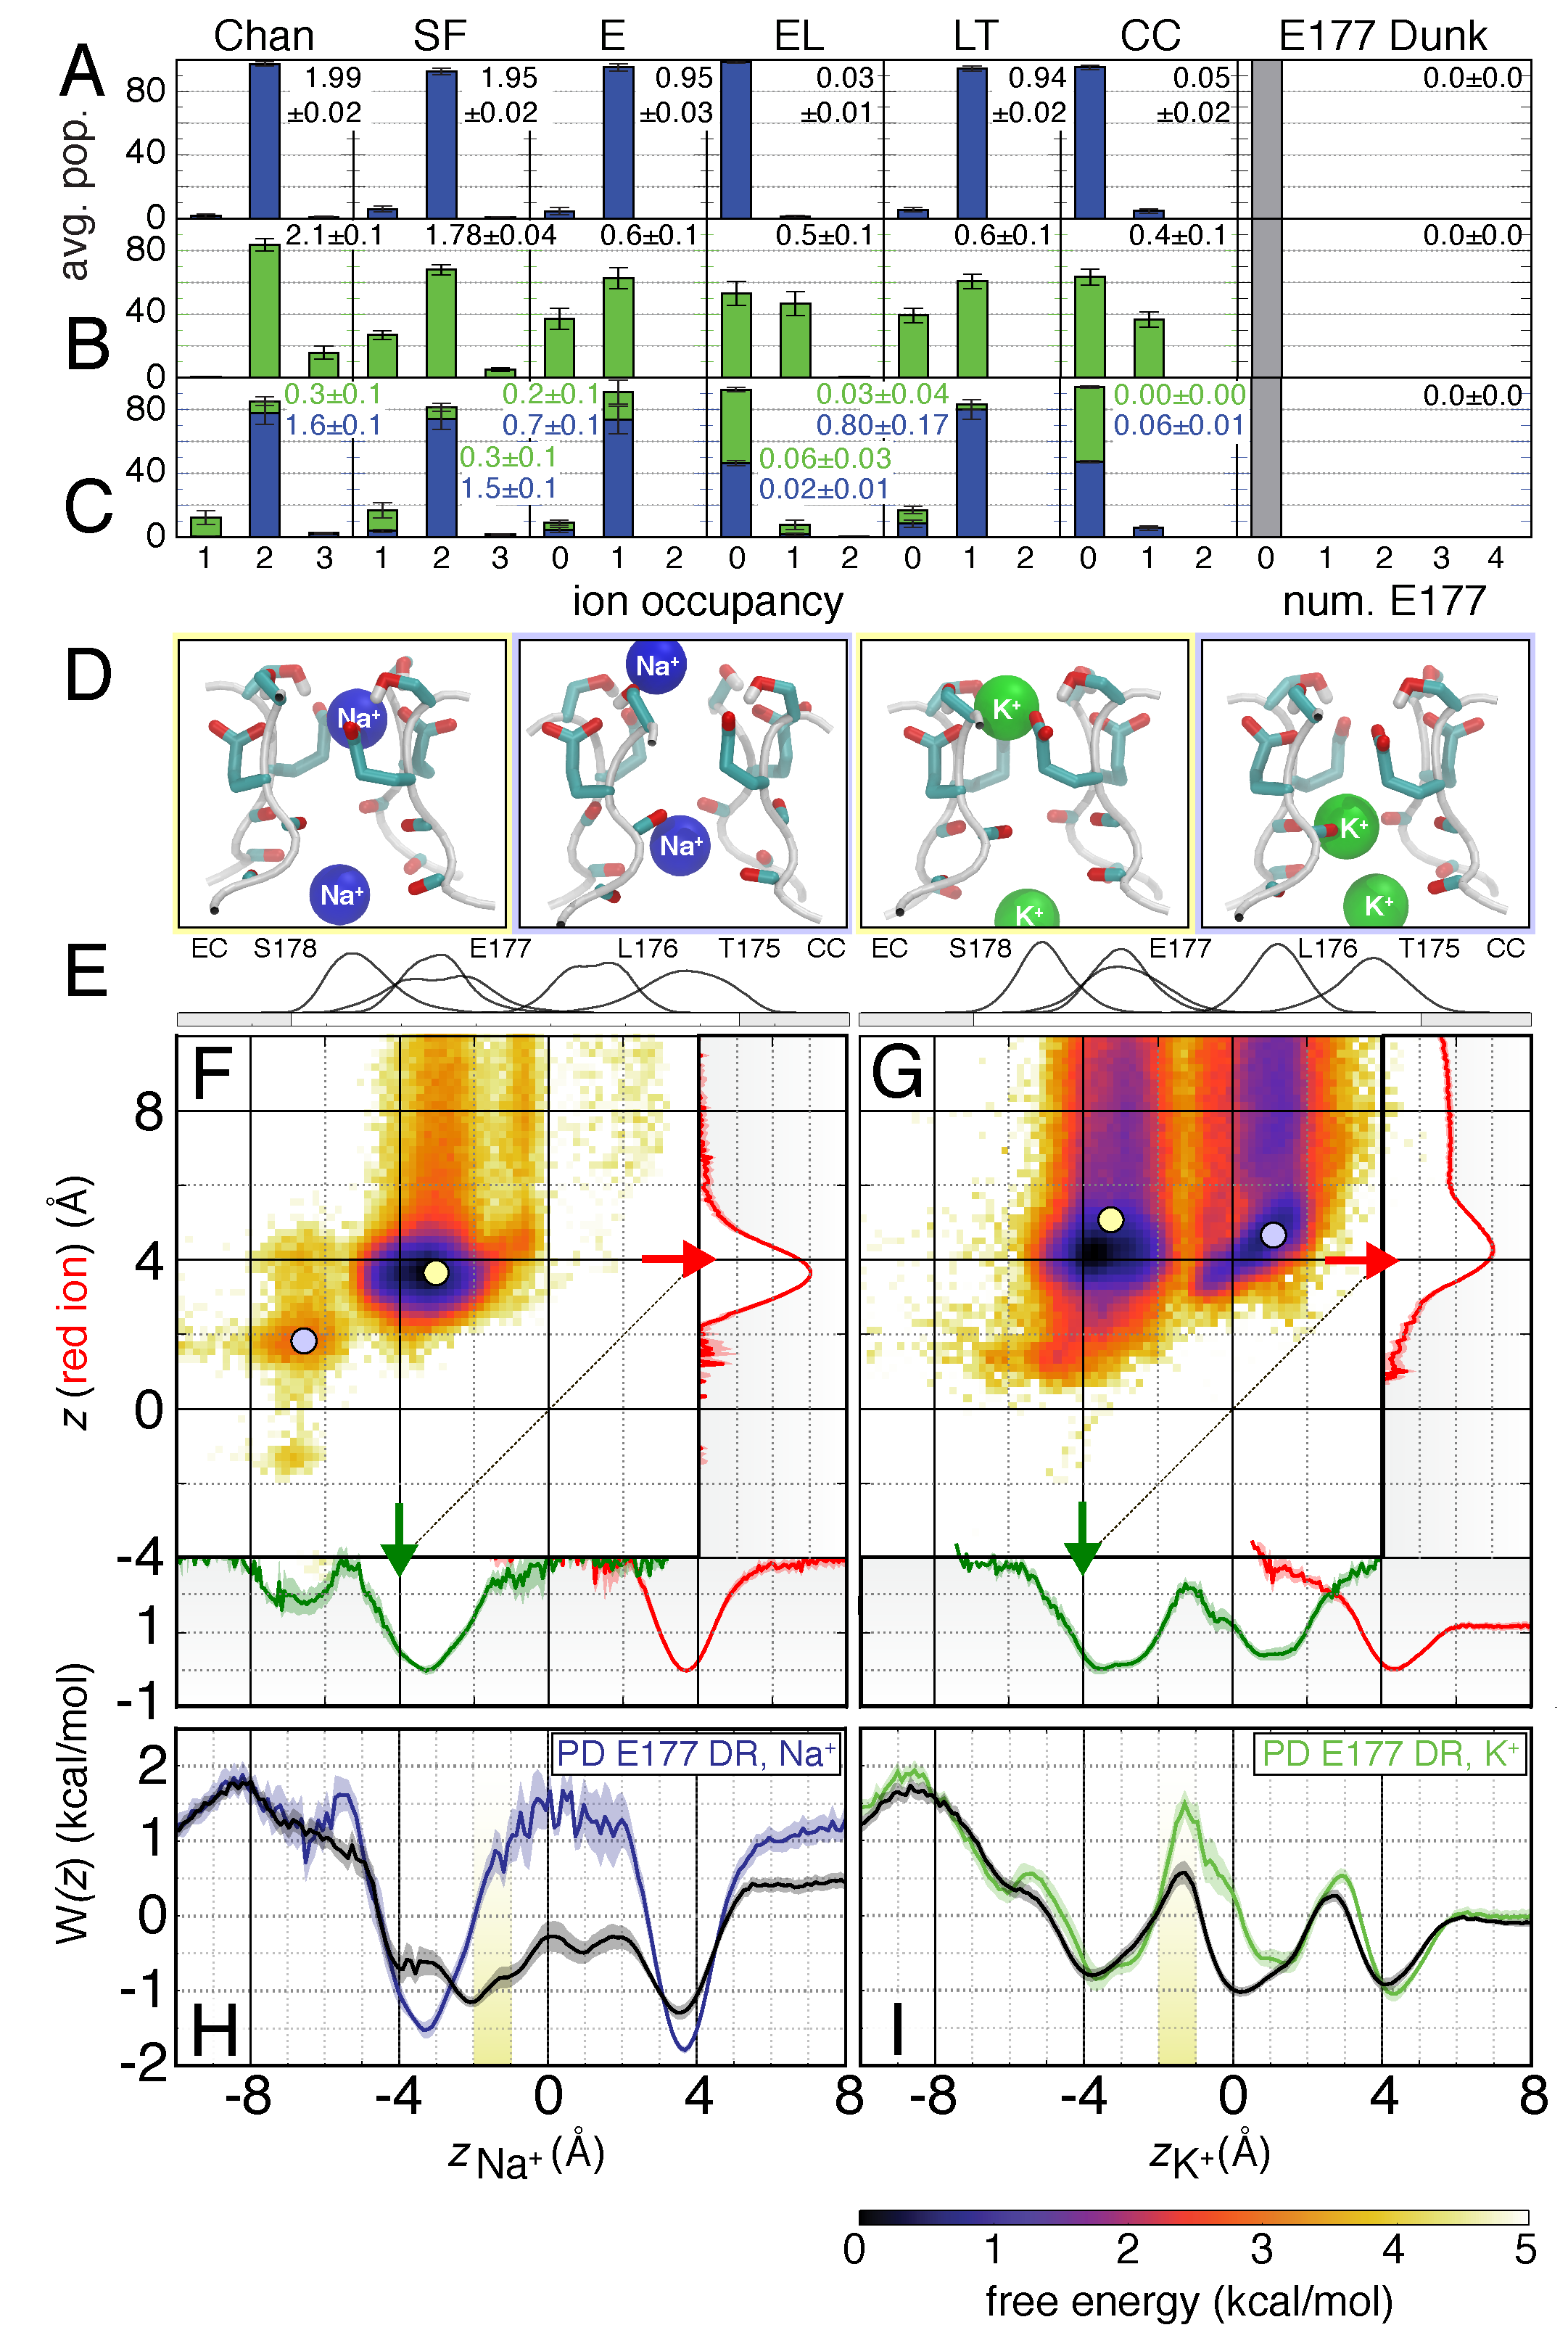
\includegraphics[width=0.6\textwidth]{nav2/Nav2Fig5}
\caption[Binding statistics and potential of mean-force (PMF) for the movement of Na$^+$ and K$^+$ along the channel axis where E177 is restrained in the crystallographic orientation]{\textbf{Binding statistics and potential of mean-force (PMF) for the movement of Na$^+$ and K$^+$ along the channel axis where E177 is restrained in the crystallographic orientation}. (\textbf{A}) Ionic occupancy is shown from left to right for the entire channel, the SF, all major binding sites within the SF, together with the number of dunked E177 side chains, for (\textbf{A}) pure Na$^+$, (\textbf{B}) pure K$^+$, and (\textbf{C}) mixed cation simulations. Values from mixed cation simulations may not reflect equilibrium distributions due to limited ion mobility. (\textbf{D}) Representative snapshots of dominant ion configurations within the SF. (\textbf{E}) The axial distribution of pore-lining oxygen atoms of T175, L176, E177, and S178 for pure Na$^+$ and pure K$^+$ simulations. 2D PMFs for (\textbf{F}) Na$^+$ and (\textbf{G}) K$^+$ are computed between red and green ion pairs for the 2 ion occupancy state. Multi-ion 1D projection onto the channel axis for E177 restrained for (H) Na$^+$ and (I) K$^+$, where a black line in each plot is the 1D PMFs for Na$^+$ and K$^+$ where no restrained were applied, respectively.}
\label{fig:nav2fig5}
\end{figure}

The ionic occupancy of the SF and the probability of E177 dunking are within statistical uncertainty for both simulations with NaCl and KCl (Fig. \ref{fig:nav2fig2} B). As such, it is unclear if E177 conformational isomerization is required for permeation and mediating selectivity. We investigate the influence of E177 side chain conformational fluctuations by restraining them in the crystallographic up-facing orientation (Fig. \ref{fig:nav2fig2} A (right panel)). In E177 restrained simulations, the average channel occupancy is comparable for Na$^+$ and K$^+$, at $2.0\pm0.02$ and $2.1\pm0.1$, respectively. There is a significant drop in occupancy of the 3 ion state for Na$^+$ ($97\pm1$ and $1.6\pm0.4$\% for the 2 and 3 ion states, respectively) and K$^+$ ($84\pm4$ and $16\pm4$\% for the 2 and 3 ion states, respectively) relative to the PD+VSD and PD models without restraints (Fig. \ref{fig:nav2fig5} A,B). For Na$^+$, this decrease in occupancy results from the elimination of binding at the `EL' site (from $0.6\pm0.1$ to $0.03\pm0.01$) which is somewhat compensated by increased occupancy of the `E' and `LT' sites. For K$^+$, ion binding persists at all sites, although what we refer to the `EL' site, by convention, now involves only coordination to L176. For Na$^+$ and K$^+$ in pure and mixed systems, triple occupancy of the SF is significantly reduced (Fig. \ref{fig:nav2fig5} A-C), but occurs transiently to induce knock-on ion permeation through the SF, shown for selected time trajectories (Fig. \ref{fig:nav2figS3} B,D,F). In mixed cation simulations, the axial distribution of Na$^+$ and K$^+$ positions were qualitatively the same as pure cation simulations in this model, but due to reduced mobility of Na$^+$ in the SF, the sampling of unique ion configurations was limited (Fig. \ref{fig:nav2figS3} C,E,G). 
2D PMFs for red/green ions reveals the extent to which the mechanism for permeation holds for Na$^+$ and to a lesser extent for K$^+$. The red and green Na$^+$ adopt a single conformation in `E' and `LT' sites (Fig. \ref{fig:nav2fig5} F), where the exit of the red Na$^+$ into the CC is rarely sampled. This is a dramatic perturbation of the free energy landscape for Na$^+$ movement, permitting only single-file conduction, compared to the liquid-like free energy surface described previously (Fig. \ref{fig:nav2fig3} A). For K$^+$, the ions can interconvert between the `E'/`LT' and `EL'/`LT' states (Fig. \ref{fig:nav2fig5} G), readily allowing red K$^+$ movement into the `CC'. The free energy barrier for green K$^+$ movement has doubled to 2 kcal/mol, but the free energy surface is otherwise qualitatively similar to 2 K$^+$ occupancy state previously described (Fig. \ref{fig:nav2fig3} B). Regions of low energy were not located on the diagonal for pure or mixed cation systems, indicating that multiple ions could not occupy the same axial position. Positional swaps of ions were not observed for Na$^+$ in pure or mixed systems, however, infrequent swaps were observed in pure K$^+$ trajectories when ions were occupying the `EL' and `LT' sites. 

\subsection{Effect of Glu to Asp mutation on cation binding}

\begin{figure}[hp]
\centering
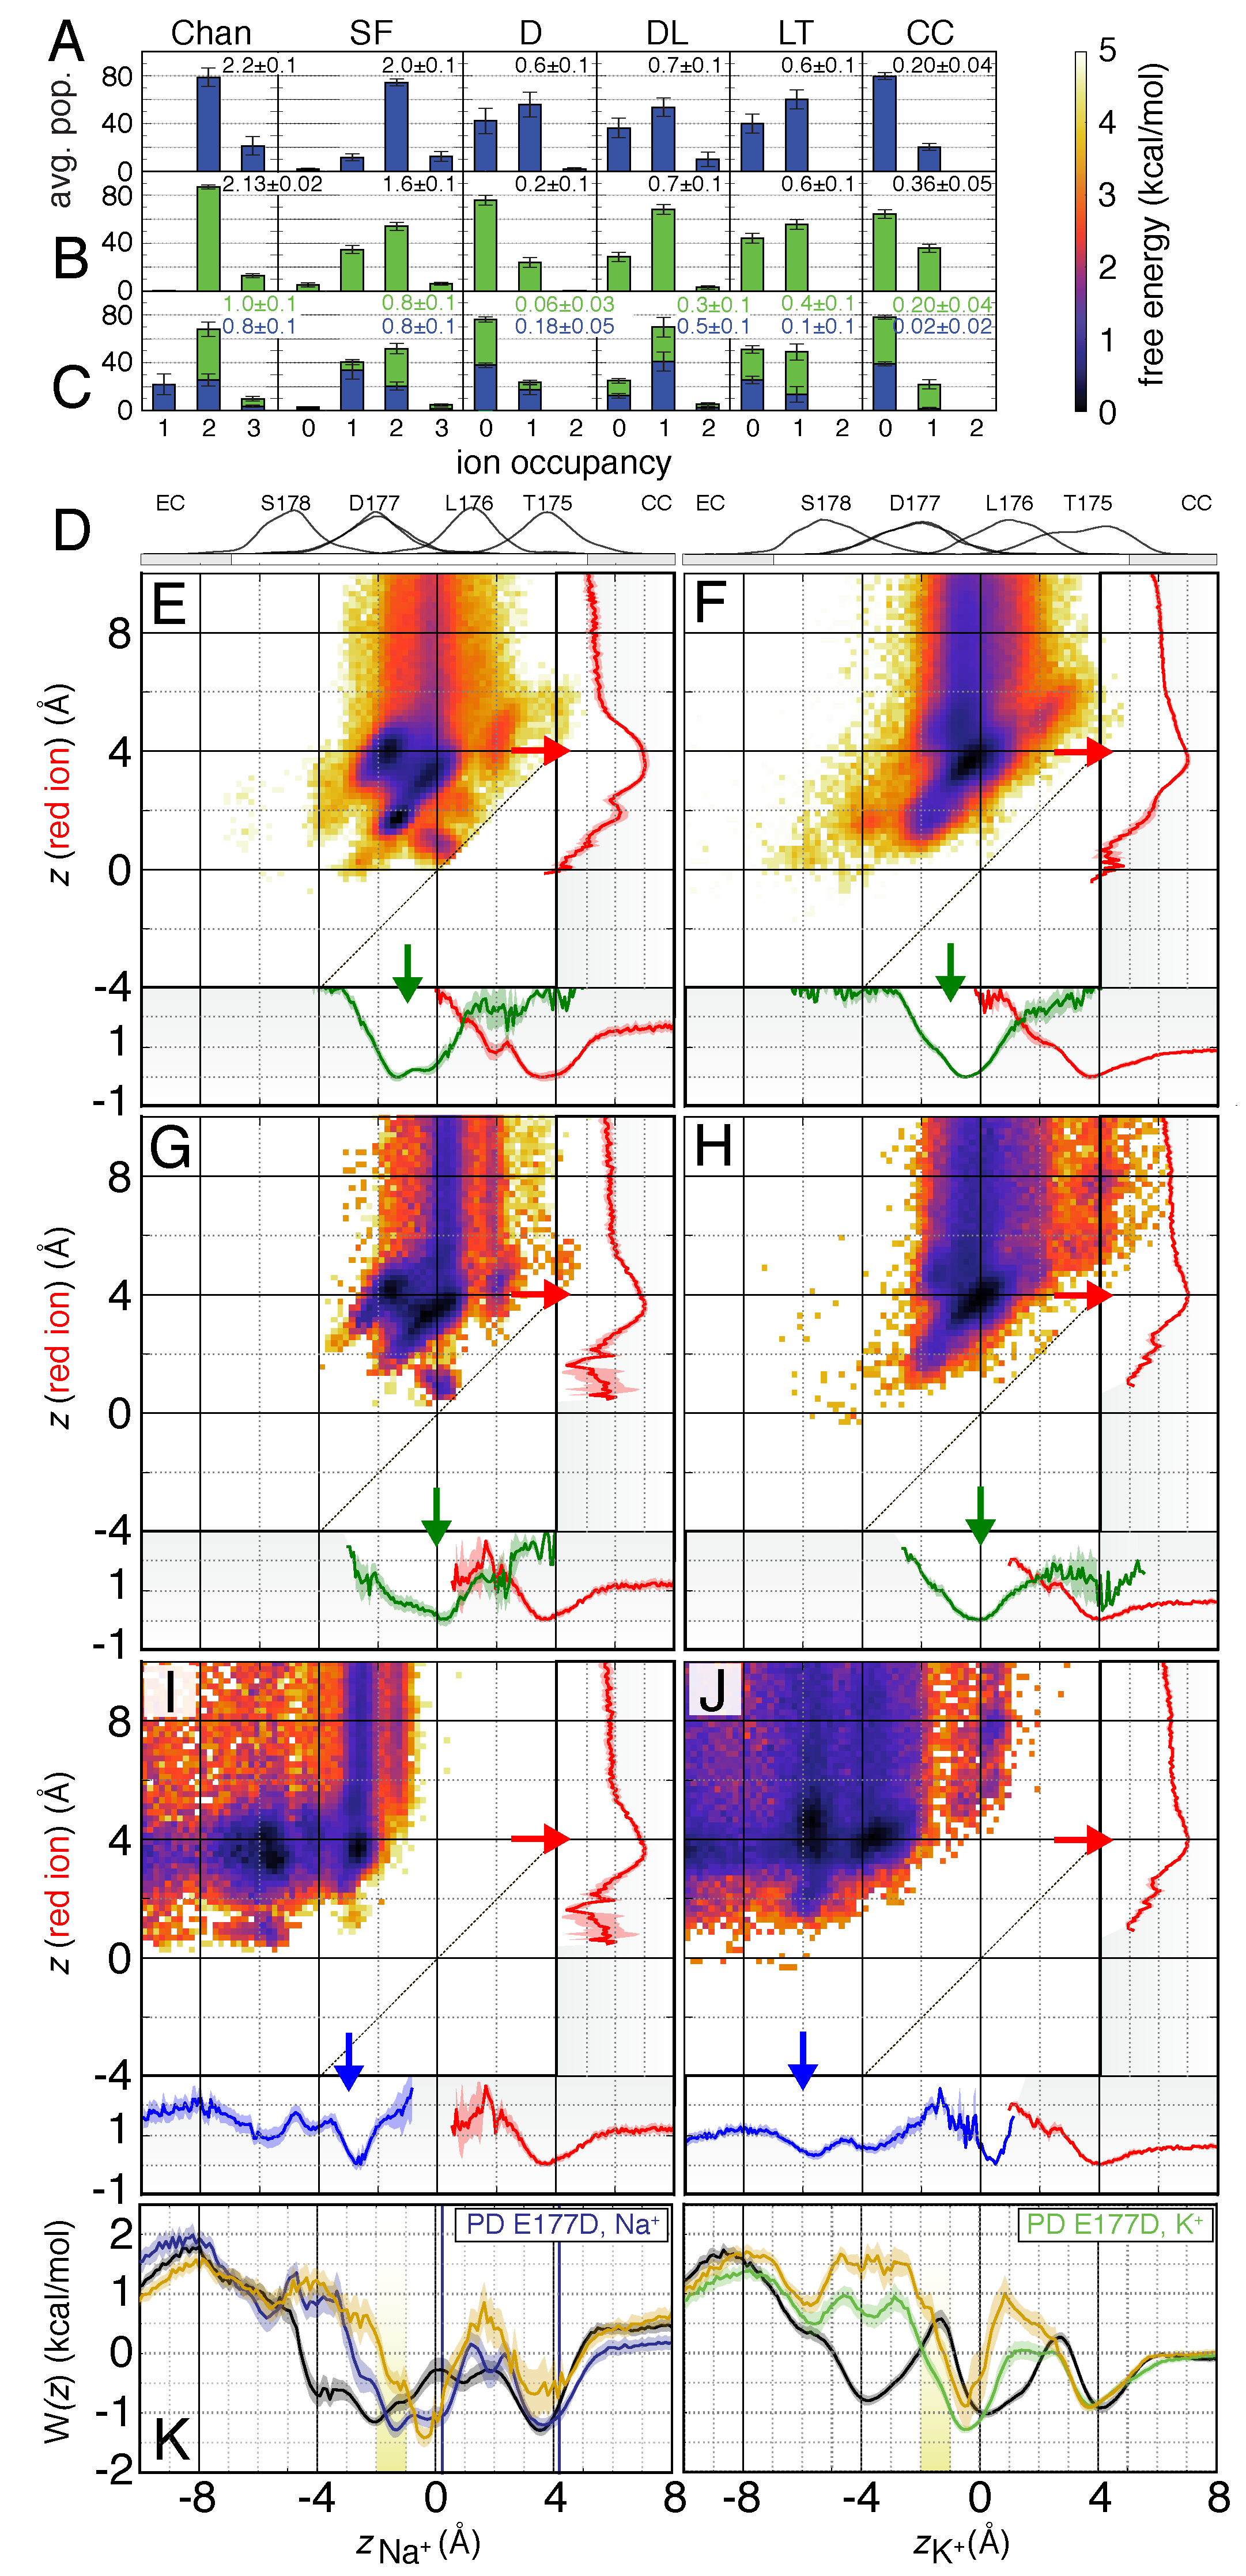
\includegraphics[width=0.6\textwidth]{nav2/Nav2Fig6}
\caption[Binding statistics and potential of mean-force (PMF) for the movement of Na$^+$ and K$^+$ along the channel axis in the E177D model]{\textbf{Binding statistics and potential of mean-force (PMF) for the movement of Na$^+$ and K$^+$ along the channel axis in the E177D model}. Ionic occupancy is shown from left to right for the entire channel, the SF, all major binding sites within the SF, together with the number of dunked E177 side chains, for (\textbf{A}) pure Na$^+$, (\textbf{B}) pure K$^+$, and (\textbf{C}) mixed cation simulations. (\textbf{D}) The axial distribution of pore-lining oxygen atoms of T175, L176, E177, and S178 for pure Na$^+$ and pure K$^+$ simulations. 2D PMFs for Na$^+$ and K$^+$ are computed between red and green ion pairs for the (E, F) 2 ion and (G,H) 3 ion occupancy state. 2D PMFs for (I) Na$^+$ and (J) K$^+$ are shown for the innermost and outermost ions, red and blue, respectively, for the 3 ion state. Multi-ion 1D projection onto the channel axis for pure (K) Na$^+$ and (L) K$^+$ (blue and green, respectively), with a black line showing the free energy of ion conduction for Na$^+$ and K$^+$ in the WT PD model as a reference. Na$^+$ and K$^+$ in mixed cation simulations are shown as a gold line in both panels.}
\label{fig:nav2fig6}
\end{figure}

\begin{figure}[!ptb]
\centering
\includegraphics[width=0.7\textwidth]{nav2/Nav2FigS6}
\caption[Conformational isomerization of residue 177 side chains]{\textbf{Conformational isomerization of residue 177 side chains}. 2D potential of mean force (PMF) for side chain torsions ($\chi_1$, $\chi_2$) of E177 with representative snapshots showing main conformers from each dataset. These conformers are rendered for two opposite subunits from the SF, corresponding to coloured circles labelled on the plots (purple, yellow, red, green). (\textbf{A}) Free energy profiles for ($\chi_1$, $\chi_2$) of E177 in the (left) PD+VSD and (middle) PD model in the presence of a mixture of Na$^+$ and K$^+$. 2D PMF plots for D177 side chain dihedral angles in the presence of pure Na$^+$ with a representative snapshot. Free energy profiles for ($\chi_1$, $\chi_2$) of E177 in the (\textbf{B}) HNNN model. In the HNNN model, the 2D PMF is calculated for subunit 1 (the protonated side chain, showing a representative snapshot) and subunits 2-4 (all deprotonated), in the presence of pure Na$^+$, as well as subunits 1-4 in the presence of pure K$^+$ (with the same protonation states). In-set boxes show the total percentage of data in two regions of $\chi_1$, $\chi_2$ space, corresponding to `undunked' and `dunked' conformations from top to bottom, separated by a dashed black line, in the WT and OPLS models. In the HNNN model, all boxes except the top left region represent a `dunked' conformation.}
\label{fig:nav2figS6}
\end{figure}

Simulations using a Na\textsubscript{V}Ab model with the sidechain shortening E177D mutation enable the study of ion conduction and selectivity under conditions where the diameter of the SF is effectively modified without changing the SF backbone. This mutation was found to reduce the Na$^+$:K$^+$ selectivity ratio to approximately 2:1 in the channel NaChBac \cite{FinolUrdaneta:2014bz}. E177D mutants crystallized of NavMs provided evidence that Na$^+$ binding may be eliminated in the outer binding site of the SF \cite{Naylor:2016cu}. In our simulations, the average channel occupancy for Na$^+$ and K$^+$ did not drop compared to WT models. However, the roughly balanced populations of the 2 and 3 ion states in the WT model shifted in favor of the 2 ion state for K$^+$ ($87\pm2$ and $13\pm2$\% for the 2 and 3 ion states, respectively) while Na$^+$ remained nearly unchanged ($76\pm8$ and $21\pm8$\% for the 2 and 3 ion states, respectively) (Fig. \ref{fig:nav2fig6} A,B). In both 2 and 3 ion states, the primary binding sites of the green and red ions are `DL' and `LT'. There is a significant loss of binding affinity at the `D' site (formerly `E', at -4 \AA) for the green ion (Fig. \ref{fig:nav2fig6} E-H, \ref{fig:nav2figS4} H,I), which is most pronounced for the green K$^+$, which no longer binds at the two sites (Fig. \ref{fig:nav2fig3} A-B). Reduction of D177-only binding occurs because the D177 sidechain is not long enough to  hold an upfacing conformation completely away from the channel lumen (where $\chi_2$ now refers to symmetric rotation about the C-C bond, Fig. \ref{fig:nav2figS6} B). Nonetheless, the previously described mechanisms of ion conduction are still possible for Na$^+$ and K$^+$ in pure cation E177D systems, with the exception that both the 2 and 3 ion states may support two Na$^+$ at the same axial position (at position $\sim$0 \AA). Specifically, the loosely knock-on mechanism in which 3 ion occupancy lowers the free energy barrier for the red ion to enter the `CC' holds also holds in the E177D mutant.
Na$^+$ and K$^+$ channel occupancy in mixed cation simulations are within error ($0.8\pm0.1$ and $1.0\pm0.1$, for Na$^+$ and K$^+$, respectively, Fig. \ref{fig:nav2fig6} C), in contrast with the marked preference for Na$^+$ over K$^+$ in the WT PD model ($1.6\pm0.1$ and $0.8\pm0.1$, for Na$^+$ and K$^+$ channel occupancy, Fig. 4H). As qualitatively compared using the 1D PMF, the primary features, namely well-depths and barrier heights, of the free energy profile are identical for Na$^+$ and K$^+$ conduction in pure and mixed cation simulations (Fig. \ref{fig:nav2fig6} I,J). Peak solvation of Na$^+$ and K$^+$ by carboxylate groups drops from $\sim$3 to $\sim$2 in this mutant (Fig. \ref{fig:nav2figS5} E,F). All ion pair 2D PMFs show that it is possible for Na$^+$ to pass itself in pure and mixed cation simulations, but it is never observed at the same axial position as K$^+$ in mixed cation simulations (Fig. \ref{fig:nav2figS7-5} F-J). Here we also show that there is no preferential binding of Na$^+$ or K$^+$ in mixed salt solutions. Our simulations show that the E177D mutation makes the channel non-selective by reducing K$^+$ binding affinity to the `D' site. 

\begin{figure}[!ptb]
\centering
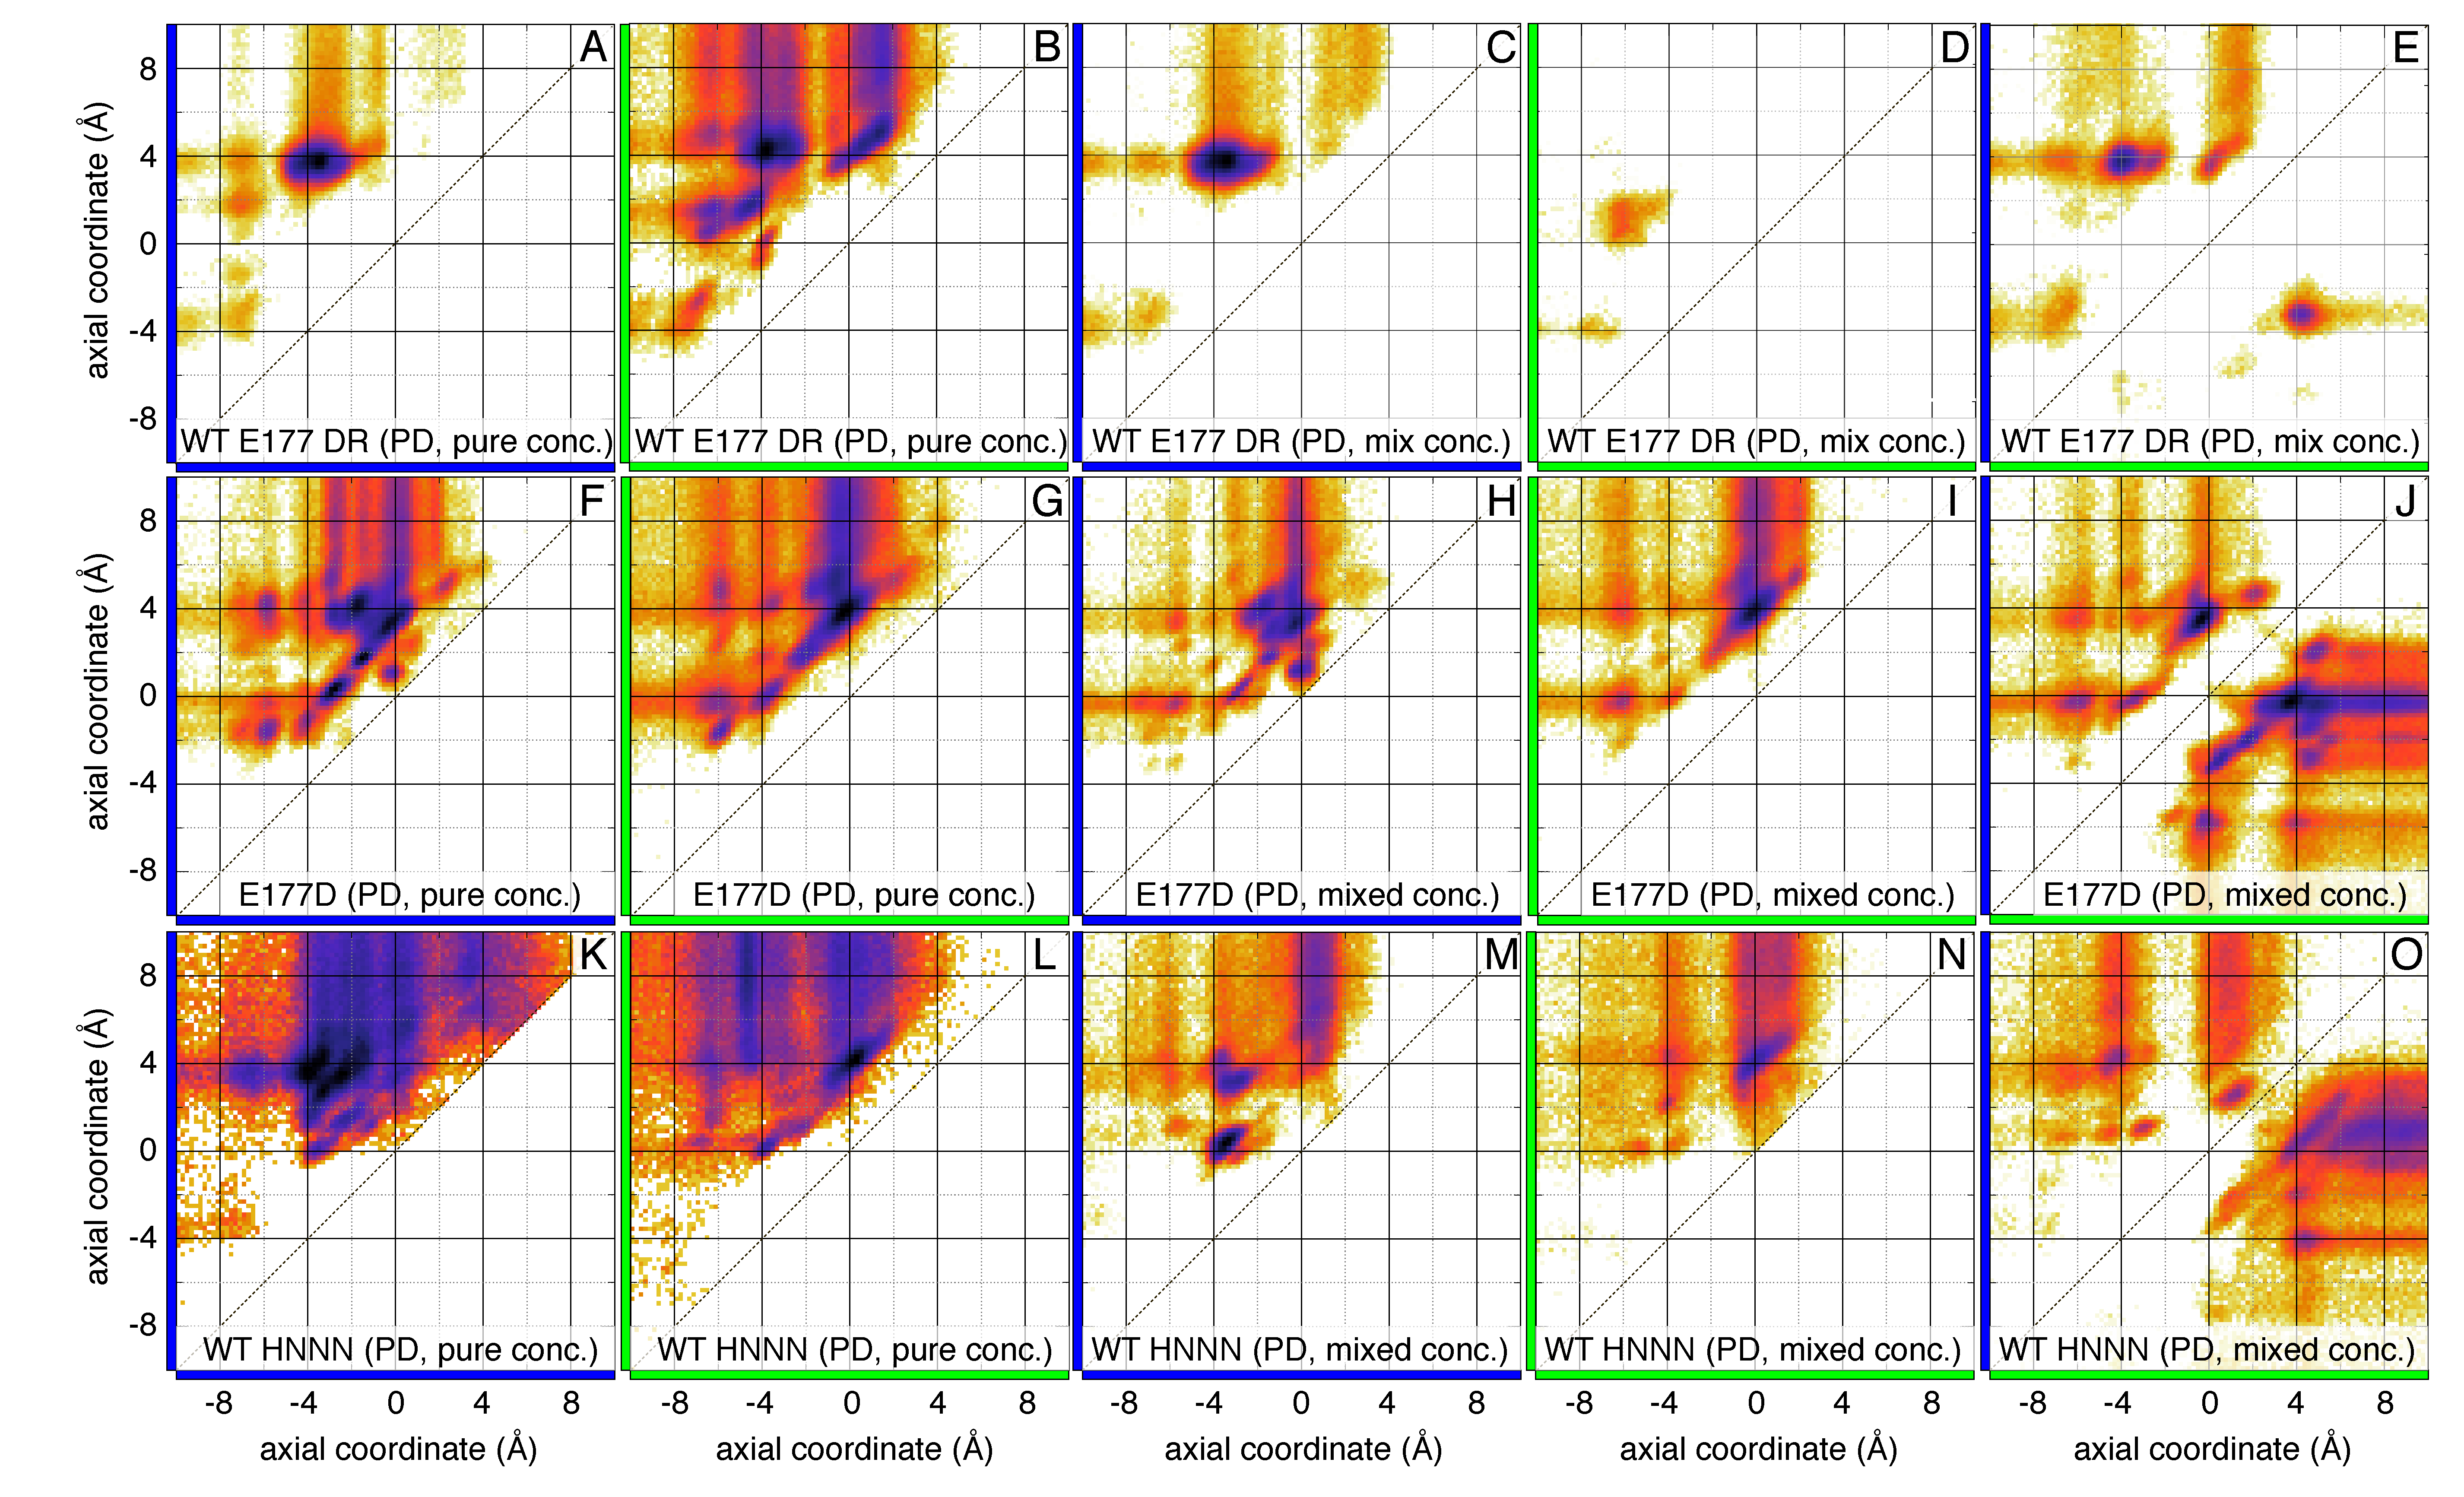
\includegraphics[width=0.7\textwidth]{nav2/Nav2FigS7-5}
\caption[Additional two-dimensional potential of mean-force (PMF) for Na$^+$ and K$^+$ pairs along the channel axis]{\textbf{Additional two-dimensional potential of mean-force (PMF) for Na$^+$ and K$^+$ pairs along the channel axis}. Ionic species are identified by a colored bar on the axes, Na$^+$ (blue) and K$^+$ (green). PMFs for (\textbf{A}) Na$^+$-Na$^+$ and (\textbf{B}) K$^+$-K$^+$ in pure cation simulations, and (\textbf{C-E}) Na$^+$-Na$^+$, K$^+$-K$^+$, and Na$^+$-K$^+$ in mixed cation simulations in the PD model with E177 dihedral restraints. (\textbf{F}) Na$^+$-Na$^+$ and (\textbf{G}) K$^+$-K$^+$ in pure cation simulations, and (\textbf{H-J}) Na$^+$-Na$^+$, K$^+$-K$^+$, and Na$^+$-K$^+$ in mixed cation simulations in the E177D model. (\textbf{K}) Na$^+$-Na$^+$ and (\textbf{L}) K$^+$-K$^+$ in pure cation simulations, and (\textbf{M-O}) Na$^+$-Na$^+$, K$^+$-K$^+$, and Na$^+$-K$^+$ in mixed cation simulations in the HNNN singly protonated E177 model. The reference state (zero free energy) is set to the high probability state for each pure cation or mixed cation simulation dataset, respectively.}
\label{fig:nav2figS7-5}
\end{figure}

\subsection{Effect of E177 protonation}

\begin{figure}[hp]
\centering
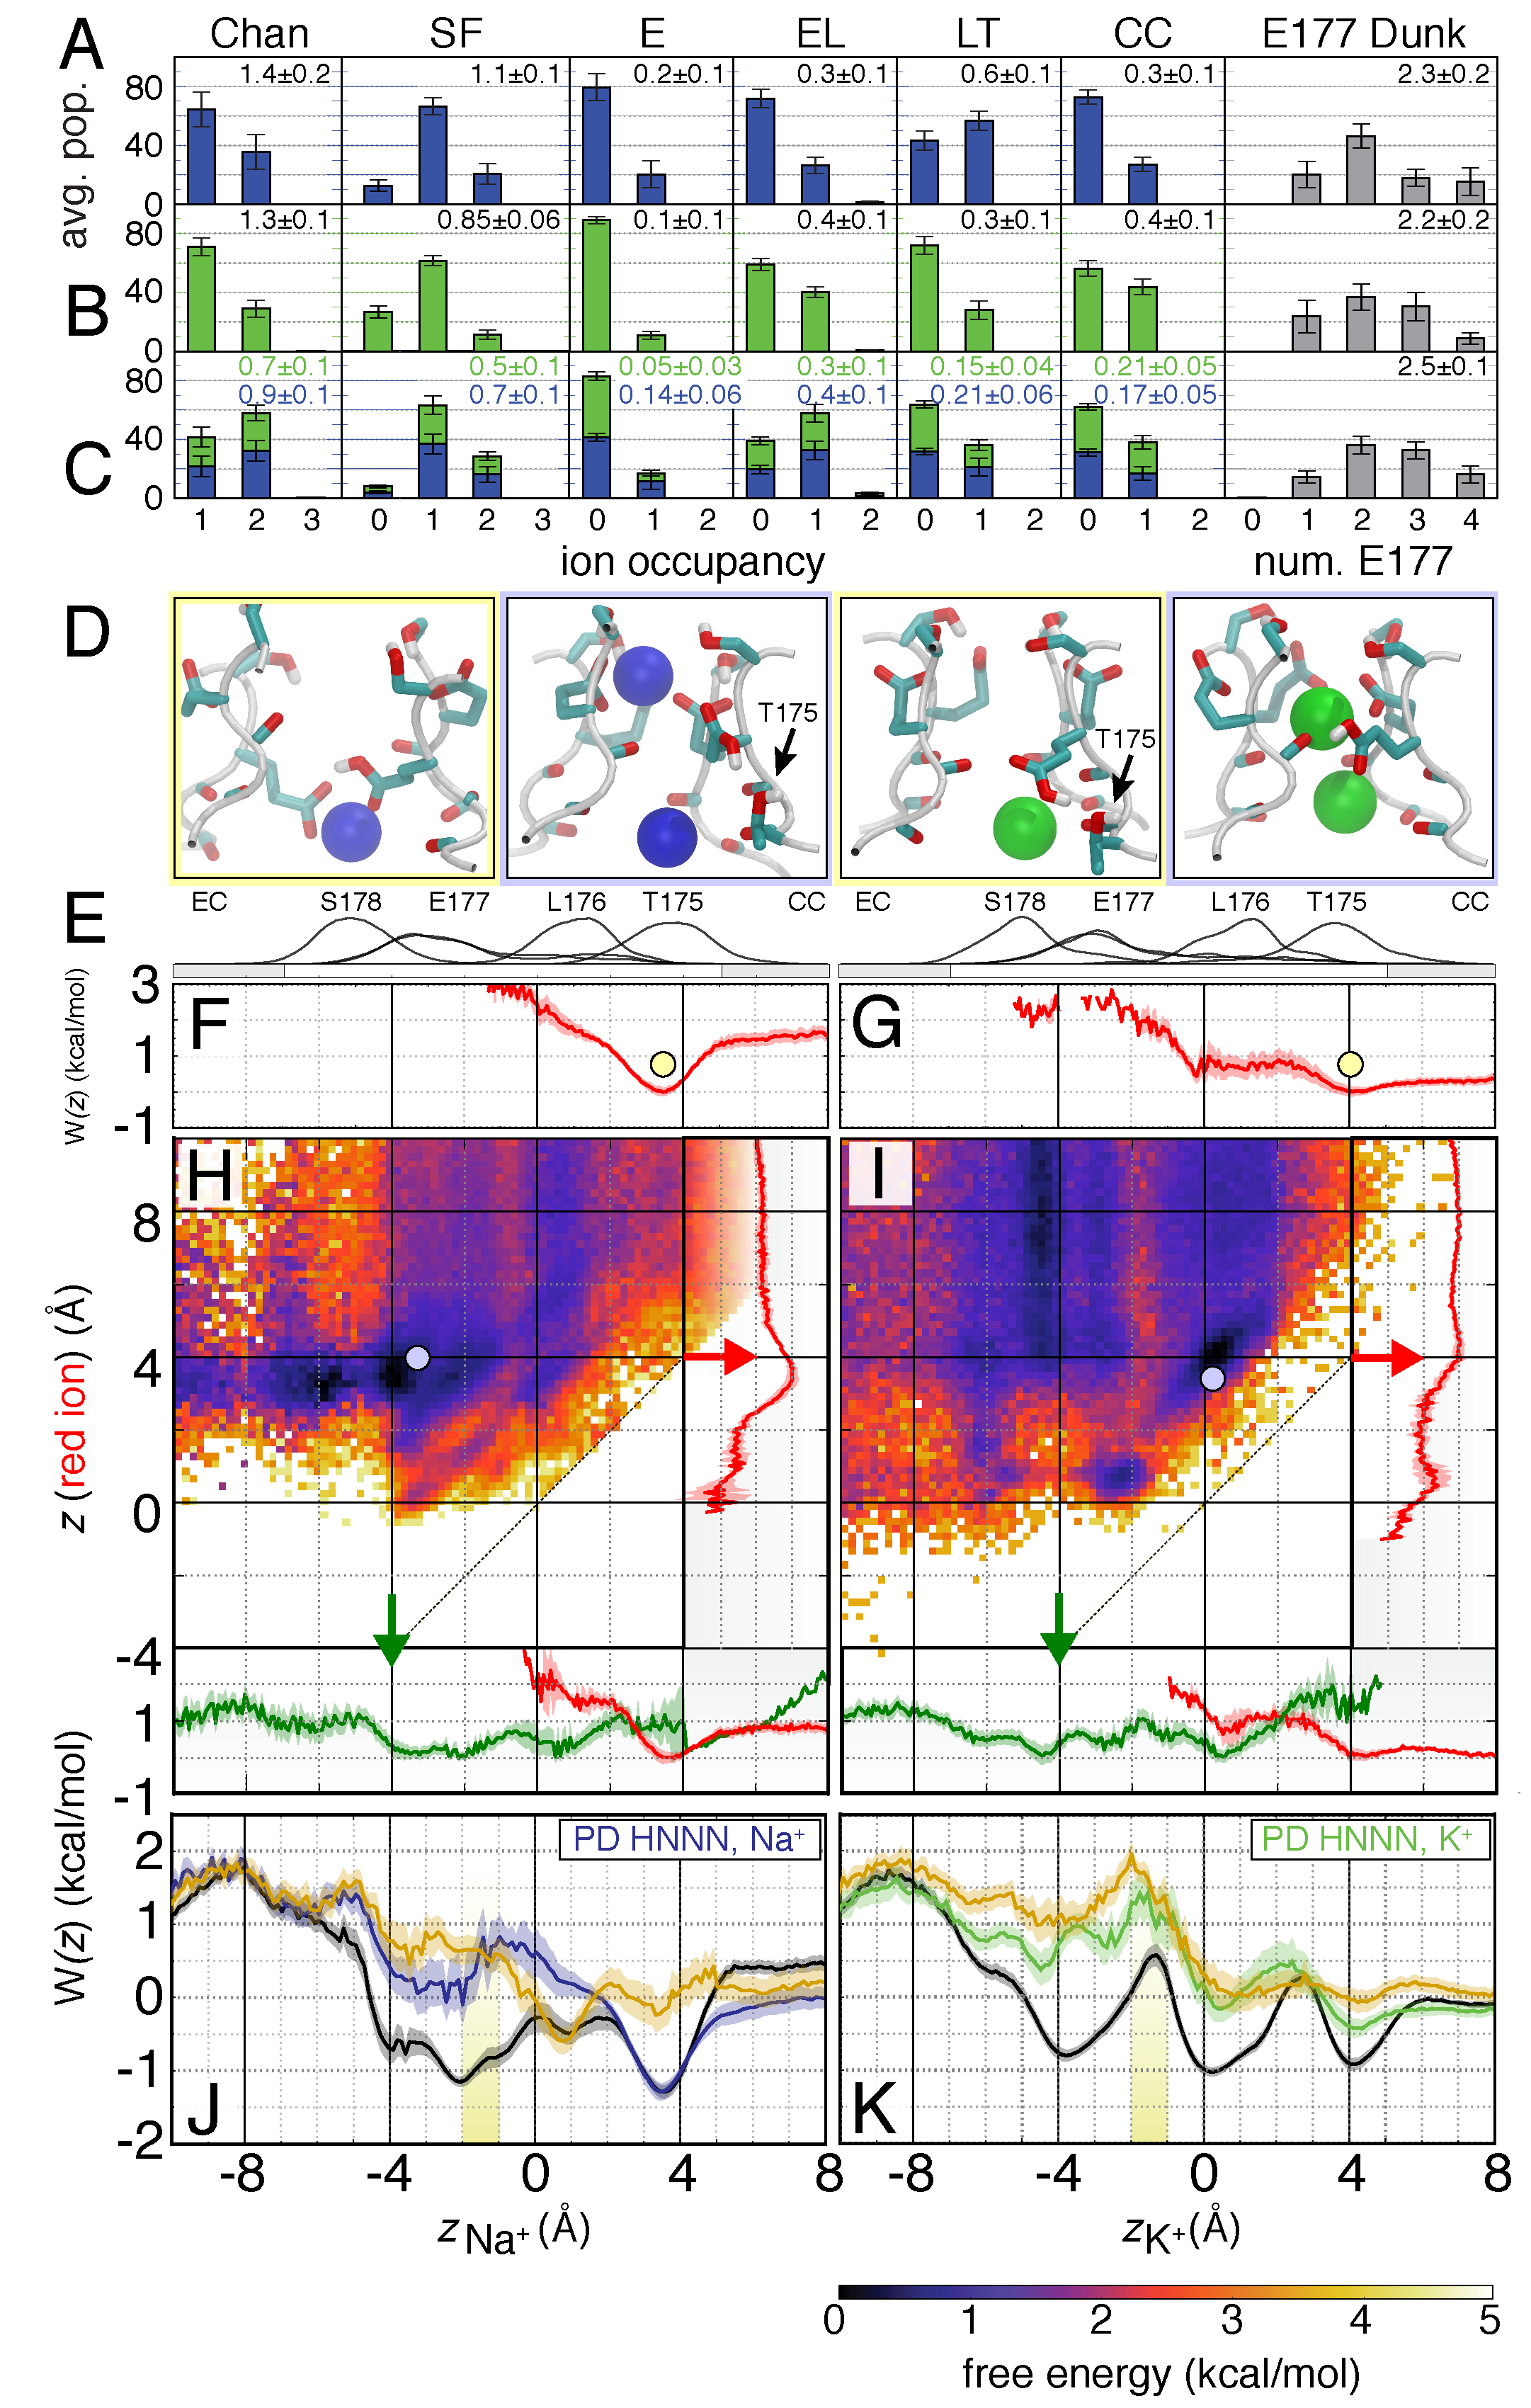
\includegraphics[width=0.6\textwidth]{nav2/Nav2Fig7}
\caption[Binding statistics and potential of mean-force (PMF) for the movement of Na$^+$ and K$^+$ along the channel axis in the single E177 protonated model]{\textbf{Binding statistics and potential of mean-force (PMF) for the movement of Na$^+$ and K$^+$ along the channel axis in the single E177 protonated model}. Ionic occupancy is shown from left to right for the entire channel, the SF, all major binding sites within the SF, together with the number of dunked E177 side chains, for (\textbf{A}) pure Na$^+$, (\textbf{B}) pure K$^+$, and (\textbf{C}) mixed cation simulations. (\textbf{D}) Representative snapshots of dominant ion configurations within the SF. (\textbf{E}) The axial distribution of pore-lining oxygen atoms of T175, L176, E177, and S178 for pure Na$^+$ and pure K$^+$ simulations. 1D PMFs for (\textbf{F}) Na$^+$ and (\textbf{G}) K$^+$ in the 1 ion occupancy state. 2D PMFs for Na$^+$ and K$^+$ are computed between red and green ion pairs for the (\textbf{H, I}) 2 ion occupancy state. Multi-ion 1D projection onto the channel axis for pure (\textbf{J}) Na$^+$ and (\textbf{K}) K$^+$ (blue and green, respectively), with a black line showing the free energy of ion conduction for Na$^+$ and K$^+$ in the WT PD model as a reference. Na$^+$ and K$^+$ in mixed cation simulations are shown as a gold line in both panels.}
\label{fig:nav2fig7}
\end{figure}

Experimental studies have shown that lowering the external pH from 7.4 to 5.8, presumably reducing the net anionic charge of the SF via protonation of one or more E177 side chains, results in a drop of Na$^+$ over K$^+$ selectivity from $\sim$33:1 to $\sim$7:1 in bacterial Na$^+$ channel NaChBac \cite{FinolUrdaneta:2014bz}. To test the influence of E177 protonation on cation permeation and selectivity, we performed simulations in which a single E177 sidechain was protonated. Protonation of the carboxylate group increased overall dunking affinity (Figs. \ref{fig:nav2fig7} A-C) and enabled the E177 side chain to adopt a large number of $\chi_1$,$\chi_2$ conformations unobserved in any other simulations, including those that permitted E177 coordination to ions bound in the `LT' binding site (Figs. \ref{fig:nav2fig7} D, \ref{fig:nav2figS6} C). Single E177 protonation resulted in a decrease of SF occupancy by $\sim$1 cation for both Na$^+$ and K$^+$ in pure cation simulations (Fig. \ref{fig:nav2fig7} A-B). Protonation decreases channel occupancy by $\sim$1 cation for Na$^+$ ($64\pm11$ and $32\pm11$\% for the 1 and 2 ion state populations, respectively) and K$^+$ ($71\pm6$ and $29\pm6$\% for the 1 and 2 ion state populations, respectively) (Fig. \ref{fig:nav2fig7} A,B). Binding of Na$^+$ and K$^+$ at `E' site is reduced by a factor of $\sim$4 and at the `EL' site by a factor of $\sim$2 when compared to the pure cation simulations in the PD system. In the 1 and 2 ion occupancy state, the red ion binds at the `LT'/`CC' site, where increased occupancy results in a lower free energy barrier to enter the `CC' for Na$^+$ (Fig. \ref{fig:nav2fig7} F-I). The green Na$^+$ and K$^+$ traverse a relatively flat free energy landscape wherein the entry of the red ion into the CC can occur at nearly any position (Fig. \ref{fig:nav2fig7} H-I). 
Although ion binding was reduced for both ions with respect to the fully deprotonated EEEE ring, the SF retained a small preference for Na$^+$ over K$^+$ in `E' and `EL' binding sites in mixed cation simulations. This minor preference for Na$^+$ over K$^+$ can be seen qualitatively in the 1D pseudo-PMF (Fig. \ref{fig:nav2fig7} H-I). Our simulations show that single E177 protonation reduces Na$^+$ selectivity over K$^+$.

\section{Discussion}

\subsection{Molecular Mechanism of Na$^+$ Selectivity}

The above results lead to four primary conclusions: 
\begin{itemize}
\item Na$^+$ and K$^+$ bind with similar stoichiometry in the SF of Na\textsubscript{V}Ab, with multiple binding modes involving a variable number of cations and a variable number of carboxylate groups of E177 side chains.
\item Conformational isomerization of E177 side chains is necessary to catalyze the conduction of Na$^+$ through the SF, whereas K$^+$ does not require E177 fluctuations to facilitate conduction. 
\item When the two types of cations compete with each other at equal concentrations, K$^+$ binding affinity is reduced at all SF binding sites in favor of Na$^+$. 
\item Selectivity for Na$^+$ originates from a difference in the multi-ion mechanism of ion translocation for Na$^+$ and K$^+$. 
\item Both side chain length reduction and reduction of anionic charge in the SF has the capacity to reduce binding affinity and selectivity for Na$^+$ over K$^+$.
\end{itemize}

The capability of the SF to provide a liquid-like free energy landscape for Na$^+$ but not for K$^+$ has its basis in the interaction between carboxylate side chains and the two ions. More effective coordination of Na$^+$ by E177 compared to K$^+$ is consistent with the concept of ionic field strength, whereby the carboxylate group is a classic high-field-strength ligand favoring the smaller cation, Na$^+$, over K$^+$ (difference in Pauling radii of 1.33 - 0.95 = 0.38 \AA) \cite{Eisenman:1962dy}.  Similarly, the preference for Na$^+$ over K$^+$ in the Na1 site of the LeuT transporter was recently ascribed to a carboxylate group from the leucine substrate \cite{Yu:2010dj} along the principle of the field-strength model.  A recent MD study of the SF of a mammalian NaV channel, in which the residues of the DEKA locus were inserted into the prokaryotic NaV channel, NaVRh, also attributed selection of Na$^+$ over K$^+$ ions in part to interactions with Asp and Glu side chains in the SF \cite{Xia:2013dv}. However, our analysis of average ionic coordination of Na$^+$ and K$^+$ within the SF shows that channel and water oxygen coordination of individual ions are not significantly different, and thus are unlikely to be the sole determinant for selectivity. Consistent variations in ion coordination between Na$^+$ and K$^+$ within the SF would support a previously proposed model for Na$^+$ selectivity \cite{Corry:2012ge}, but our results do not support this model. Likewise, even though we did not employ non-equilibrium methods, in competitive binding we do not observe evidence for K$^+$ block of Na$^+$ within the SF as described in a previous study \cite{Ngo:2016es}.  

Although the SF of Na\textsubscript{V}Ab is wider than that of K$^+$ channels in the absence of dunking \cite{Payandeh:2012ib}, conformational isomerization of the side chains of E177 in the confined environment of the SF creates a flexible binding site that appears to be well suited for the preferential binding of Na$^+$ relative to K$^+$. In particular, the SF supports multiple Na$^+$, often side-by-side, whereas this does not occur for K$^+$. At a physical level, this may still be due to the difference in ionic radius of the two ions, where K$^+$ is too large to fit into an ionic cluster coordinated by multiple E177 side chains. In turn, these results suggest that the conformational flexibility of the Glu side chains favors a loosely-coupled conduction mechanism, ultimately resulting in Na$^+$ selectivity.

\subsection{Model Limitations}

In our previous Nav channel simulation study \cite{Chakrabarti:2013kd}, we computed Na$^+$ conductance in a closed channel model, and found this to be on the same order of magnitude as experimental estimates (1-10 million ions/sec). These calculations were performed on the basis of identical relative free energy inside the central cavity versus the bulk, no evidence for interactions between the SF and the contents of the CC, and the assumption that crossing the IC gate would occur faster than crossing the SF in an open channel. In the current pure and mixed simulation datasets presented in this work, we no longer have equal affinity for ions in the central cavity and the SF and `LT'/`CC' sites are never occupied simultaneously (Fig. \ref{fig:nav2fig2} B-C,  \ref{fig:nav2fig4} H), confirming that `CC' occupancy influences SF binding. However, the `CC' occupancy in our simulations (0.2-0.3 with a bulk ionic concentration of 247 mM, Fig. \ref{fig:nav2fig2} B), was comparable to the CC occupancy of an open K$^+$ channel (0.24 with a bulk K$^+$ concentration of 140 mM) \cite{Sumikama:2016kb}, suggesting that our simulations of the closed-state may still recover the binding affinity of the `CC' in the open-state. Regardless of `CC' occupancy, we determined several qualitative features, robust to simulation force field, which support a molecular mechanism for $\sim$2-fold selectivity of Na$^+$ over K$^+$. These findings, particularly those pertaining to the role of glutamic acid side chains in selectivity, are unlikely to be altered in a model of the open-state channel given that the open-state SF is unchanged from the closed-state structure used in our simulations. 

\subsection{Comparison to Previous Computational and Experimental Studies}
Even though electron density corresponding to Na$^+$ was not identified within the SF of the Na\textsubscript{V}Ab I217C structure used in this study \cite{Payandeh:2012ib}, three highly occupied Na$^+$ binding sites were observed in the SF of a homologous 2.7 \AA NavMs structure \cite{Naylor:2016cu}. These binding sites correspond roughly to positions of the proposed S$_{HFS}$, S$_{CEN}$, and $S_{IN}$ sites. Previous simulation studies disagree on the number of binding sites within the SF, reporting two \cite{Chakrabarti:2013kd,Furini:2012jl}, three \cite{Boiteux:2014ut,Corry:2012ge}, four \cite{Domene:2015kj,Ke:2014fy}, or five Na$^+$ binding sites \cite{Stock:2013cg,Ulmschneider:2013da}, which also differ in axial position. In this work, we identified three primary Na$^+$ binding sites defined by ionic coordination to residues `E', `EL', and `LT' (Fig. \ref{fig:nav2figS4}). These sites are in qualitative agreement with the binding sites observed in the NavMs SF \cite{Naylor:2016cu}. 

Accurate simulations of a bacterial Nav channel should reproduce electrophysiological conductance (1-10 million ions/sec) and selectivity measurements ($\sim$10:1 Na$^+$ over K$^+$). Even for well-studied channels, such as gramicidin and KcsA, simulations underestimate experimental conductance \cite{Allen:2004vs,Jensen:2013gn}. Although the calculated conductance and selectivity from one NavMs channel simulation study were on the correct order of magnitude for Na$^+$ and K$^+$ \cite{Ulmschneider:2013da}, our work challenges several findings from this manuscript. In our simulations with E177 restrained in the crystallographic conformation, we observed greatly reduced binding at the `EL' site, resulting in an axial distribution of ions very similar to the one presented in that work \cite{Ulmschneider:2013da}. These discrepancies must be due to methodological differences between our study and Ulmschneider et al., namely; an open-state pore-domain model, structural restraints, and external applied voltage. However, a systematic study is required in order to pin point the source of this discrepancy. 

Our understanding of selectivity in Nav channels is further strengthened by examining SF modifications that reduce Na$^+$ selectivity. Results from E177D simulations indicate that both the binding affinity and the conduction mechanism are similar for Na$^+$ and K$^+$ in pure and mixed cation models, in a manner consistent with electrophysiological and computational studies showing that the E177D mutant is poorly selective \cite{FinolUrdaneta:2014bz}. Our simulations in pure and mixed cation E177 protonated models are also consistent with the decrease in Na$^+$:K$^+$ selectivity measured in the same study \cite{FinolUrdaneta:2014bz}. Pure cation simulations of Na$^+$ in this model are in agreement with previous PMF calculations showing changes in E177 conformational isomerization and a large decrease in binding at the `E' site of the channel \cite{Furini:2014gv}. Inversely, our results do not agree with an unbiased equilibrium simulation reporting that the singly-protonated SF had a comparable free energy of Na$^+$ conduction to the fully charged EEEE ring  \cite{Boiteux:2014ut}.

Future calculations of conductance in a stable open-state Nav channel structure may assist in better understanding the role of channel fluctuations (in the SF and TM regions), multi-ion effects, and voltage on conductance and selectivity. Such studies should provide complimentary information to the mechanistic description of ion movement through the SF in pure and mixed cation concentrations, potentially reweighting the populations of states observed within the SF in our simulations to offer a more complete picture of Na$^+$ selectivity.

\section{Methods} 

\subsection{Molecular Modelling and Simulation} 

Multiple all-atom molecular models were constructed using the Na\textsubscript{V}Ab I217C structure (PDB code: 3RVY) \cite{Payandeh:2012ib} (Fig. S1). The three models employed in this study (named PD, PD+VSD, and OPLS PD+VSD), with the exception of the voltage sensor domains, differ primarily in the size of the simulation cell. %A summary of all molecular models and simulation datasets are presented in Table S1.

In the PD+VSD model, all transmembrane domains of the Na\textsubscript{V}Ab I217C structure (S1-S6, residue 1-221) were embedded in a hydrated 1,2-dimyristoyl-sn-glycero-3-phosphatidylcholine (DMPC) bilayer (270 lipid molecules) with a NaCl or KCl concentration of 247 mM. Both N- and C-terminal ends of the protein were modeled as neutral moieties. This simulation cell was comprised of $\sim$129,000 atoms with approximate dimensions of 10.8 $\times$ 10.8 $\times$ 11.3 $nm^3$. Membrane embedding was performed using alchembed \cite{Jefferys:2015jt} with an equilibrated CHARMM36 DMPC bilayer patch obtained from the Jeffery Klauda laboratory website (https://terpconnect.umd.edu/$\sim$jbklauda/research/download.html). The protein, lipids, and ions were modeled with the CHARMM36 all-atom force field \cite{Best:2012kb,Best:2012uu,MacKerell:1998tp,Klauda:2010tn}, and water molecules were modelled with TIP3P \cite{Jorgensen:1983ty}. NBFIX adjustments were made for Na$^+$ - backbone carbonyl oxygen atom interactions \cite{Noskov:2008jp}, as well as NBFIX corrections for Na$^+$ - lipid head group interactions \cite{Venable:2013ix} (note that equivalent Na$^+$ - protein carboxylate group interactions were not used since not equivalent parameterization was available for K$^+$). 

All PD+VSD and PD simulations were performed with GROMACS 4.6.5 \cite{Hess:2008db} using the same simulation settings. Electrostatic interactions were calculated using particle-mesh Ewald \cite{Essmann:1995vj,Darden:1993vu} with a real-space cut-off distance of 1.2 nm, a grid spacing of 0.16 nm, and cubic interpolation. Lennard-Jones interactions were cut off at 1.2 nm. Nonbonded interactions were calculated using Verlet neighbor lists \cite{Verlet:1967cm}. All simulations were performed at constant temperature (300 K) and pressure (1 atm) using the Nos\'e-Hoover thermostat \cite{Hoover:1985wf,Nose:1984em} with temperature coupling of 0.5 ps and the Parrinello-Rahman barostat \cite{Nose:1983cu,Parrinello:1980uc} with a time constant of 2 ps, respectively. All chemical bonds were constrained using the LINCS algorithm \cite{Hess:2008fl}. The integration time step was 2 fs. 

For both NaCl and KCl concentrations, steepest descent minimization was used to ensure forces less than 1000 kJ mol$^{-1}$ nm$^{-2}$, followed by three successive NPT simulations of 10ns to assist in equilibration. In these equilibration steps, position restraints were applied to heavy atoms, main chain backbone atoms, and then C$\alpha$ atoms, with restraint strength of 1000 kJ mol$^{-1}$ nm$^{-2}$. Fifteen simulation repeats were then generated with randomized initial velocities for both NaCl and KCl concentrations, and run for 1,000 ns. Across both NaCl and KCl, an aggregate total of 30 $\mu$s was performed using the PD+VSD model.

In the PD model, the pore domain of Na\textsubscript{V}Ab (S5-S6, residue 130-221) was embedded in a hydrated DMPC bilayer with a salt concentration of 240 mM. Both N- and C-terminal ends of the protein were modeled as neutral moieties. A hydrated DMPC lipid patch of 200 lipids in 150mM NaCl was generated using CHARMM-GUI \cite{Wu:2014uc} and equilibrated under NPT for 20 ns with the CHARMM36 force field \cite{Klauda:2010tn}. Membrane embedding was performed using g_membed \cite{Wolf:2010dr} where 14 lipid molecules were removed. This resulted in a periodic rectangular cell comprised of $\sim$61,000 atoms with approximate dimensions of 8.3 $\times$ 8.3 $\times$ 8.3 nm$^3$. In mixed cation simulations of the PD model, the salt concentration was 197 mM for both NaCl and KCl. Using the identical pure and mixed cation models, additional systems were constructed with modifications made to the EEEE ring, including the E177D mutation and the protonation of a single E177 side chain. The protein, lipids, and ions were modeled with the CHARMM36 all-atom force field \cite{Best:2012kb,Best:2012uu,MacKerell:1998tp,Klauda:2010tn}, and water molecules were modelled with TIP3P \cite{Jorgensen:1983ty}, identical to the parameters used for PD+VSD simulations above.

An alternative PD+VSD model was used in simulations of the OPLS force field \cite{Jorgensen:1996vx,Kaminski:2001eq}. This system has a larger simulation cell comprised of $\sim$219,000 atoms in total, with approximate dimensions of 16.7 $\times$ 16.7 $\times$ 9.8 nm$^3$. The OPLS NaCl dataset used in this work is identical to the one utilized in our previous manuscript \cite{Chakrabarti:2013kd}, and we generated a new OPLS KCl dataset using an identical modelling and simulation protocol. In this system, the protein was modeled with the OPLS-AA/L all-atom force field \cite{Jorgensen:1996vx,Kaminski:2001eq} with default ions parameters \cite{Aqvist:1990ud}, the lipid bilayer was modelled with Berger parameters \cite{Berger:1997bc}, and water was modelled with the TIP3P model \cite{Jorgensen:1983ty}. 

Forty-seven simulations of 400-500 ns each as well as forty-eight 500-ns simulations yielded 21.6 and 24 $\mu$s of simulation data for NaCl and KCl simulations. A set of ten 250 ns NaCl simulations was performed using the same OPLS NaCl model with the addition of E177 side chain dihedral restraints, ($\chi_1$,$\chi_2$) = (210 degrees, 290 degrees), with a force constant of 5000 kJ mol$^{-1}$ rad$^{-2}$. Simulations were performed with GROMACS 4.0.7 \cite{Hess:2008db}. 

Mixed cation simulations in the OPLS PD+VSD model were performed in two stages, where only the latter stage is presented in this study. With equal concentrations of 150mM NaCl and 150 mM KCl, we observed that systematic errors in the ion parameters of the OPLS forcefield resulted in significant Na$^+$ binding to the lipid head group region. This resulted in a decrease of bulk ionic concentration of Na$^+$ from an expected 150mM to approximately 90mM. Bulk ion concentration of K$^+$ in competition studies was also larger than 150mM at approximately 190mM. Due to the importance of equal sodium and potassium for competitive binding studies, we performed fifty additional competition simulations of 300ns (15 $\mu$s) where this bias was corrected. Initial conditions for these corrected concentration runs were carefully selected in order to reproduce the expected populations of the EL, E, and CC binding sites we would expect for the equal Na$^+$ and K$^+$ concentrations (approximately double the sodium binding propensity). Specifically, twenty-five initial conditions were selected from a pool of the forty-five final frames of the first set of competition runs (at approximately t=500ns). Initial conditions were randomly selected from the pool until the ratios of ionic occupancy across the ensemble (E 12:1, EL 2.5:1, CC 0.35:1) were twice that of the original competition runs (E 5.4:1, EL 1.25:1, CC 0.28:1). Water oxygens in a region outside of 30 \AA from the protein were stochastically replaced with 55 Na$^+$ atoms. Additionally, 32 K$^+$ atoms were removed to correct for the overestimate of potassium concentrations. Two replicas for each initial condition were run with differing initial velocities and identical simulation parameters to the previous runs. Significant ion binding to the surface of the bilayer was not observed with the other force fields used in this study.

\subsection{Analysis} 
Atomic positions, ionic coordination, and dihedral angles of E177 side-chains were extracted using MDAnalysis \cite{MichaudAgrawal:2011fd}. All axial positions of ions were measured relative to the center of mass of the C$\alpha$ atoms of residues 175 and 178 for all subunits at each frame (a point approximately at the center of the selectivity filter). The position and coordination of all ions within a cylinder of radius 10 \AA (with arbitrary height) was centered at the SF center of mass. To correct for tilting of the protein within the bilayer, the principal axis of all protein atoms was computed at each frame and the positions of all atoms were projected onto this axis. 
The first-shell coordination of Na$^+$ or K$^+$ were computed by counting the number of oxygen atoms within 3.0 \AA or 3.4 \AA of the ions, respectively (corresponding to the first minima in the ion-protein oxygen radial distribution function). Second-shell coordination was computed by counting the number of occurrences of a water oxygen within 3.3 \AA of a channel oxygen while having same water oxygen within 3.0 \AA or 3.4 \AA of the Na$^+$ or K$^+$, respectively, while ensuring that the cation to channel oxygen distance was larger than both of the previous two distances (this count was also checked to remove cases of double counting). 
In the analysis of channel occupancy macrostates, the total channel occupancy was defined as the count of all ions within the axial range -10 \AA to 14 \AA. Macrostate populations were not sensitive to this axial cutoff value at the `EC' or `CC' boundaries. Similarly, a removal of `EC' ions from the total channel occupancy count was not found to have a significant effect on macrostate populations or kinetics.
In binding statistics analysis, channel occupancy was defined as the count of all ions within the axial range -10 \AA to 14 \AA (inherently within a 10 \AA radius cylinder centered within the SF). We utilized first and second shell coordination to define SF occupancy as any ion bound in the `E', `EL', or `LT' binding sites. Based on first shell and second shell coordination, each ion was labelled with a respective SF binding site. Failing to find a binding site, meaning no first shell coordination, ions were classified as `EC' or `CC' based on axial position (cutoffs of -5 \AA for `EC', and 5 \AA for `CC', but populations of these states were largely insensitive to these values). S178-only coordination of ions did not occur significantly in our dataset, and the remaining S178 and E177 coordinated ions were grouped into the `E' binding site. Given the high number of degenerate binding modes within the SF of Na\textsubscript{V}Ab, numerous binding modes of ions had to be manually grouped into a site based on their dominant first-shell channel ligands and sometimes ion axial position. In the case of OPLS simulations, the `LT' binding mode could be identified based on first shell coordination only, but in all other simulations, second shell coordination was needed to define this site. 
Potentials of mean force (PMF) were computed from axial ionic distributions $\rho$(z) using the following relationship: W(z) = -k$_B$T ln $\rho$(z), where k$_B$ and T are the Boltzmann constant and the absolute temperature, respectively. Similarly, 2D PMF maps were computed from the axial ionic distributions $\rho$(z$_1$, z$_2$) of distinct ion pairs (red/green, green/blue, red/blue), or all unique ion pairs using the following relationship: W(z$_1$, z$_2$) = -k$_B$T ln $\rho$(z$_1$, z$_2$), where we ensures that z$_1$ <  z$_2$. For example, in cases of triple ionic occupancy of the channel, all-pair plots simultaneously show the free energy of red-green, green-blue, and red-blue ionic configurations (Fig. \ref{fig:nav2figS7}).
E177 side chain dihedral angles are defined as $\chi_1$ = N-C$_{\alpha}$-C$_{\beta}$-C$_{\gamma}$ and $\chi_2$ = C$_{\alpha}$-C$_{\beta}$-C$_{\gamma}$-C$_{\delta}$. The dihedral angle values from our previous work were transformed by multiplying by -1.0 and adding 360 degrees if the value was less than 0.0 \cite{Chakrabarti:2013kd}. In this work we have not multiplied the initial angles by -1. 

All time averaged properties in this manuscript were computed with data recorded at a 20 ps intervals with the exception of the PD+VSD OPLS NaCl model that was recorded at 25 ps. Equilibration time, defined as the time needed to reach stable occupancy of the channel, is taken to be 150 ns for the pure and mixed cation systems selected. This is with exception to OPLS PD+VSD mixed cation simulations where no data was removed. In this system, mixed cation simulation repeats were equilibrated for 500ns. This equilibration period was removed prior to all analysis conducted in this work. All error bars in this manuscript were computed with the standard error of mean over all simulation repeats in a given simulation set, unless otherwise specified. The average oxygen coordination in Fig. \ref{fig:nav2figS5} was computed individually over all coordination values found in an axial histogram bin. Since many replicas did not sample all positions along the channel axis, positions not sampled would otherwise lower the estimate of ion coordination. 
In the case of 1D PMF calculations, we computed error bars using the following protocol. A unnormalized histogram of ionic positions was computed with 0.11 \AA spacing for each simulation repeat. Each histogram was normalized by the number of data points in that repeat (the same value within a simulation dataset in all our calculations except for OPLS PD+VSD NaCl). Very low non-zero counts in position histograms were found to introduce a large amount of error in the average and error, so positions with less than 3 data points were flagged and replaced with NaN values for exclusion from averaging. Each PMF was shifted such that its mean bulk value in the position range -20 \AA to -19 \AA (in the extracellular bulk) was set to a free energy of zero. The mean and standard error of mean for each PMF bin was then computed and used for plotting. In 2D PMF calculations, we only report the average over all simulation repeats and error is not shown. In these plots, the reference state (zero free energy) is set to the highest probability state for each pure cation or mixed cation simulation dataset, respectively, rather than the mean bulk value.
 
%\section{Supplemental Figures} 
%\beginsupplement









%\begin{figure}[!ptb]
%\centering
%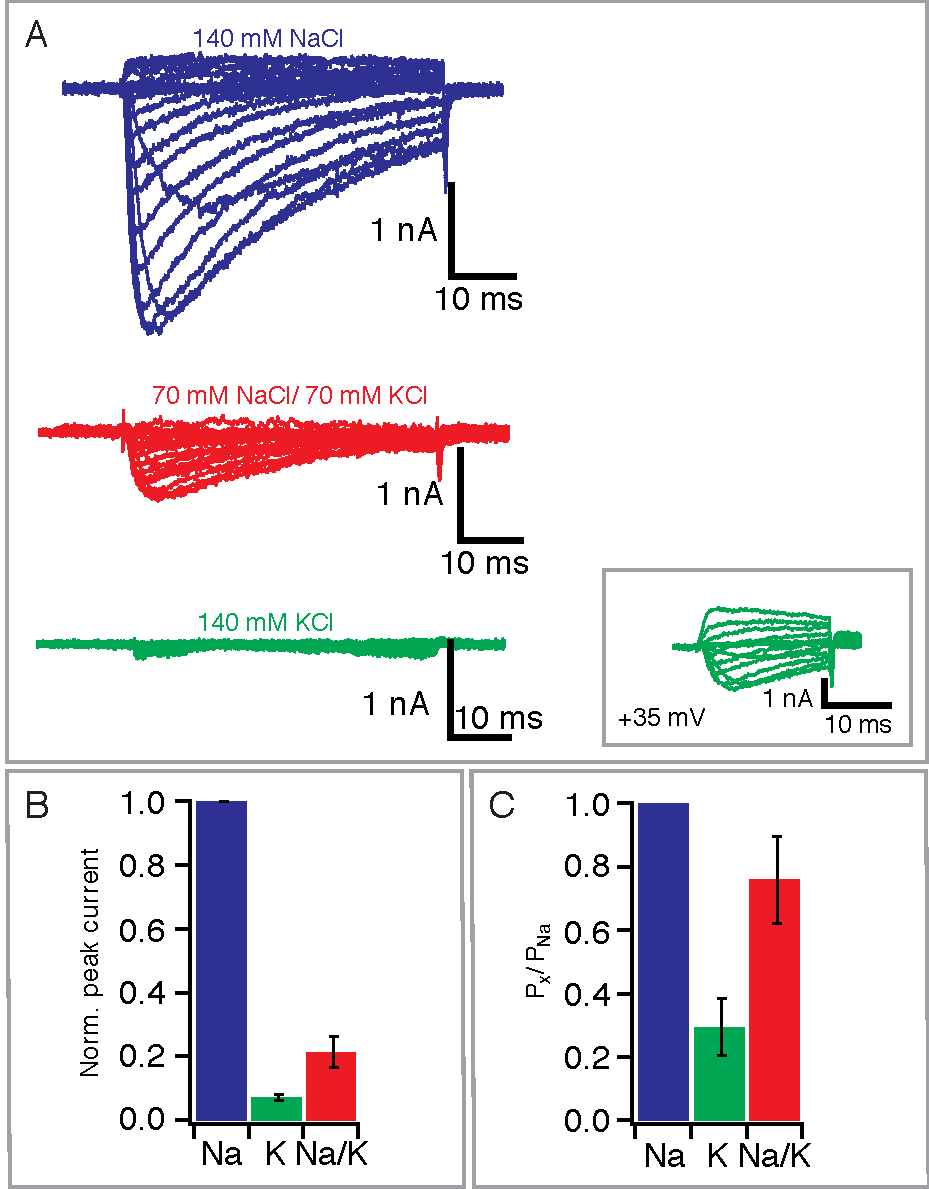
\includegraphics[width=0.7\textwidth]{nav2/Nav2FigS10}
%\caption[Na\textsubscript{V}Ab relative permeabilities measured with respect to intracellular solution containing 35 mM KCl and 105 CsF]{\textbf{Na\textsubscript{V}Ab relative permeabilities measured with respect to intracellular solution containing 35 mM KCl and 105 CsF}. (\textbf{A}) Whole cell currents using different extracellular solutions; 140 mM NaCl, 70 mM NaCl /70 mM KCl, and 140 mM KCl measured in the same cell showing the different sizes of inward currents. K$^+$ conductance was very low compared to Na$^+$ conductance or a mixture of Na$^+$ and K$^+$. Clear inward K currents were observed but only under conditions where the amount of channel expression was increased to extremely high levels (inset). (\textbf{B}) Mean peak current obtained with different extracellular solutions. (\textbf{C}) Relative permeabilities calculated from reversal potentials measured from IV curves.}
%\label{fig:nav2figS10}
%\end{figure}

\printbibliography[heading=subbibnumbered,title={References}]
\end{refsection}
\pagebreak

\begin{refsection}
\chapter{Mutations Involving Glutamic Acid Sidechains Modulate Na$^+$ Conduction}

Contributions by Christopher Ing (CI), Nilu Chakrabarti (NC), Regis Pomes (RP), and William A. Catterall (WC): C.I., N.C, and R.P. designed the research. Simulations were performed by N.C. and C.I. Data analysis was performed by C.I. and R.P. The manuscript was written by C.I., and R.P. 

\newpage

\section{Summary}

	Dynamic fluctuations of channel ligands are integral to ion permeation and selectivity in cation channels. Microsecond-timescale molecular dynamics simulations of the bacterial voltage-gated Nav channel reveal that glutamic acid side chains within the SF can adopt both a down-facing and up-facing state, and that these conformational fluctuations can catalyze Na$^+$ conduction and result in Na$^+$ selectivity over K$^+$. This process may involve variable numbers of Glu sidechains and result in coordination to a variable number of partially hydrated cations. These channel fluctuations can dynamically modulate the effective diameter and charge of the SF in response to permeating ions, and are found to catalyze the conduction of Na$^+$ by providing a diffusive free energy landscape. These fluctuations enable selective permeation of Na$^+$ by supporting multi-ion occupancy within the SF while simultaneously restricting K$^+$ movement due to geometric constraints. The role of channel fluctuations is evident from simulations where glutamic acid sidechains are conformationally restricted to an up-facing state, which does not facilitate rapid transport of Na$^+$ in agreement with experimental conductance rates. However, this molecular mechanism has not been verified experimentally.
	
	We propose mutations to the hydrogen bonding environment around these carboxylate side chains, that modulate conformational isomerization and alter ion conduction properties of Na$^+$ and K$^+$. Mutations which remove protein-protein interactions involving carboxylate sidechains to neighbouring hydroxyl sidechains of serine sidechains (S178A, S180A, S178A/S180A) are found to increase the propensity for glutamic acid side chains to adopt a down-facing state and alter ionic binding within the SF. Conversely, mutations which increase the likelihood that carboxylate sidechains will form protein-protein interactions with neighbouring serine hydroxyl groups (Y168F) are found to increase the propensity to adopt a up-facing state, and ionic conduction is found to be impeded. The Y168F mutation results in a Na$^+$ and K$^+$ conduction mechanism that is consistent with simulations conducted with conformationally restricted glutamic acid sidechains. In all systems, we examine the free energy of ion conduction for both Na$^+$ and K$^+$ and make predictions about expected perturbations to experimental observables such as ionic conduction rates and selectivity ratios. Together, this work demonstrates that the degree of conformational isomerization of glutamic acid side chains can modulate ionic conduction and selectivity, and that this prediction may be experimentally tested using site-directed mutagenesis and electrophysiology.
	
\section{Introduction}

%Voltage-gated sodium channels initiate action potentials in excitable cells through selective transport of Na$^+$ across biological membranes \cite{Hille:2001tw}. Selectivity for Na$^+$ over other biological cations like K$^+$ and Ca2+ is controlled by a narrow constriction within the ion conduction pathway referred to as the selectivity filter. 

The bacterial voltage-gated sodium channel selectivity filter is homo-tetrameric and is lined with backbone carbonyl groups, carboxylate side chains, and serine hydroxyl groups \cite{Payandeh:2012ib}. Carboxylate side chains have been identified near or within the SF of several other ion channels from disparate protein families \cite{Li:2017ex,Paulsen:2015bp,Grieben:2016ij}, but their role in ionic conduction is not well understood.  In K$^+$ channels, SF channels have been linked to ion conduction \cite{Kratochvil:2016jx,Noskov:2004tv}, and structures solved of the KcsA channel in low [K$^+$] demonstrate that the SF is also capable of collapse as a mechanism for inactivation \cite{Zhou:2001vo}. What is the extent to which SF fluctuations play a role in Na$^+$ conduction in Na$^+$ channels?

In the bacterial voltage-gated sodium channel, our previous data support the hypothesis that sidechain conformational isomerization, or dunking, plays a critical role in selective Na$^+$ conduction \cite{Chakrabarti:2013kd}. Our molecular simulations demonstrate that glutamic acid side chains are essential ligands of Na$^+$ and that their conformational isomerization is coupled to binding and movement of Na$^+$ \cite{Chakrabarti:2013kd}. Selective permeation of Na$^+$ through the SF occurs through a loosely-coupled knock-on mechanism involving 2-3 partially hydrated Na$^+$ which directly coordinate 1-4 glutamic acid sidechains. Furthermore, we've determined that by artificially preventing glutamic acid fluctuations we observe a major destabilization of Na$^+$ binding within the SF (Chapter 5). Multiple studies have since analyzed the role of glutamic acid sidechain fluctuations in Na$^+$ conduction \cite{Ke:2014fy,Boiteux:2014ut,Domene:2015kj,Furini:2014gv}. A similar mechanism has been described for the glutamate ring of the cation-selective nicotinic acetylcholine receptor \cite{Harpole:2014gu}. Our simulations also support the link between ionic selectivity and channel fluctuations. In studies of Na$^+$ and K$^+$ binding within the bacterial voltage-gated sodium channel, multi-ion occupancy of the SF results in a diffusive energy landscape for Na$^+$ but not for K$^+$. Due to geometric constraints of E177 sidechains within the SF and a difference in ionic radii, a free-energy barrier prevents rapid diffusion of K$^+$ in favour of Na$^+$. Together, these factors strengthen the connection between channel fluctuations and selective ionic conduction, but experimental evidence supporting this hypothesis has so far been scarce.

Crystallographic structures do not identify increased temperature factors for atoms within the SF. In both open and closed structures of voltage-gated sodium channels, there are only sub-angstrom variations in backbone and sidechain root-mean square deviation of the SF \cite{Sula:2017jx,Sula:2017hu,Lenaeus:2017cy} with the exception of a putative inactivated state of the NavAb channel with an asymmetrically closed SF \cite{Payandeh:2013ex}. Electron density assigned to Na$^+$ within the SF of a high-resolution crystal structure of NavMs does not indicate that glutamic acid sidechains adopt alternative conformations to coordinate bound ions \cite{Naylor:2016cu}. In the structure of the eukaryotic channel NavPas, the orientation of Asp and Glu side chains could not be assigned in the SF due to radiation damage \cite{Shen:2017df}. Nonetheless, this lack of structural evidence for channel fluctuations does not preclude dynamics of side chains under physiological conditions. On the basis of molecular dynamics simulations, can we propose channel mutations that may be used to measure the effect of E177 fluctuations on ionic conduction?

In the experiments presented here, we extend our previous studies of Na$^+$ and K$^+$ permeation in NaVAb \cite{Chakrabarti:2013kd} with simulations of novel channel mutants that modulate Na$^+$ conduction. Specifically, we perform multiple all-atom 1000-ns molecular dynamics repeats, and compare Na$^+$ binding and permeation properties of the WT channel and four mutants, S178A, S180A, S178/S180A, and Y168F. The former three mutants increase conformational isomerization and the latter mutant decreases conformational isomerization. A strong relationship is found between this propensity for E177 conformational isomerization and the binding of Na$^+$ within the SF. When drawing comparison between Na$^+$ and K$^+$, we expect that these mutants, particularly those preventing dunking, will perturb or eliminate selectivity for Na$^+$. These results provide the foundation for experimental validation of glutamic acid side chain fluctuations as a determining factor for the mechanism of conduction and selectivity in Nav channels.

\section{Results}

Channel fluctuations involving glutamic acid side chains occur spontaneously in brute-force molecular dynamics studies of the sodium channel NavAb. We have shown how binding to permeating cations displaces the conformational equilibrium towards the down-facing or dunked state of the Glu side chains \cite{Chakrabarti:2013kd}. To further characterize the factors controlling the conformational equilibrium, we analyze the protein-protein interactions involving E177. In a representative molecular rendering from simulations, we observe multiple hydrogen bonding partners for glutamic acid side chain E177 of the NavAb SF in the up-facing conformation, whereas no protein-protein hydrogen bonds were observed in the dunked state (Fig. \ref{fig:nav6fig1}) (unless one or more E177 were protonated, in which case it could form hydrogen bonds with unprotonated glutamic acid sidechains). A single E177 carboxylate group can interact with one or more serine hydroxyl groups of S178 or S180. One of these primary ligands of E177, S180, was found to interact with a neighboring Y168F side chain, preventing the hydroxyl side chain from acting hydrogen bond donor (Fig. \ref{fig:nav6fig1} A-B). Hydrogen bonds may be formed individually between E177 and S178 of the same subunit, E177 and S180 of the adjacent subunit, or both simultaneously (Fig. \ref{fig:nav6fig1} A-D). In the absence of these interactions, E177 may adopt a lumen-facing state, directly coordinating permeating Na$^+$ within the SF (Fig. \ref{fig:nav6fig1} E). In the presence of these interactions, E177 adopts an outfacing state, near the crystallographic orientation (Fig. \ref{fig:nav6fig1} F-G). 

\begin{figure}[!ptb]
\centering
\includegraphics[width=0.8\textwidth]{nav6/Nav6Fig1}
\caption[Molecular rendering of the hydrogen bonding network surrounding E177 in Na\textsubscript{V}Ab]{\textbf{Molecular rendering of the hydrogen bonding network surrounding E177 in Na\textsubscript{V}Ab}. (\textbf{A}) Structure of the NavAb selectivity filter from molecular simulation from the extracellular view, with selectivity filter residues E177, S178, and surrounding residues S180 and Y168 shown. (A-B) The crystallographic conformation of E177, hydrogen bonded to S178, along with the adjacent S180 hydrogen bonded to Y168. (C) Alternate conformation of E177, hydrogen bonded to S180, which is no longer interacting with Y168. (D) Alternate conformation of E177, hydrogen bonded to both S178 and S180. (E-H) Structure of the NavAb selectivity filter from a side-view orientation, showing (E) conformational isomerization of a single E177 side chain to coordinate ions, and (F-H) the three E177 hydrogen bonding partners shown in (A-D).}
\label{fig:nav6fig1}
\end{figure}

	Na$^+$ movement through the SF is coupled to the conformational isomerization of the side chains of E177 between an `undunked' and `dunked' state which may occur on a timescale of tens of nanoseconds \cite{Chakrabarti:2013kd}.  Specifically, cation binding shifts the conformational equilibrium of E177 from the crystallographically-observed conformer, ($\chi_1$,$\chi_2$) = (t, g$^+$), to the conformer where the carboxylate group points into the channel lumen, ($\chi_1$,$\chi_2$) = (t, g$^-$). We computed the percentage of frames where E177 adopted a dunked conformation in the presence of Na$^+$ or K$^+$ (Fig. \ref{fig:nav6fig2}). In WT simulations of Na$^+$, E177 side chains adopt a dunked conformation in 45$\pm$5\% of frames, which provides a reference value to compare our mutant channels. In the S178A and S180A mutants, E177 dunking is promoted to 83$\pm$4\% and 76$\pm$4\% of frames, respectively. By introducing both Ser to Ala mutations in the S178A/S180A mutant, E177 dunking increased to 87$\pm$3\% of frames. Conversely, the Y168F mutation promoted the interaction of E177 to S180, resulting in an overall reduction of E177 dunking to 6$\pm$2\% of frames. The percentage of dunked conformations were within error for Na$^+$ and K$^+$ for all models with the exception of S180A, which promoted dunking to 62$\pm$2\% for K$^+$. 

\begin{figure}[!ptb]
\centering
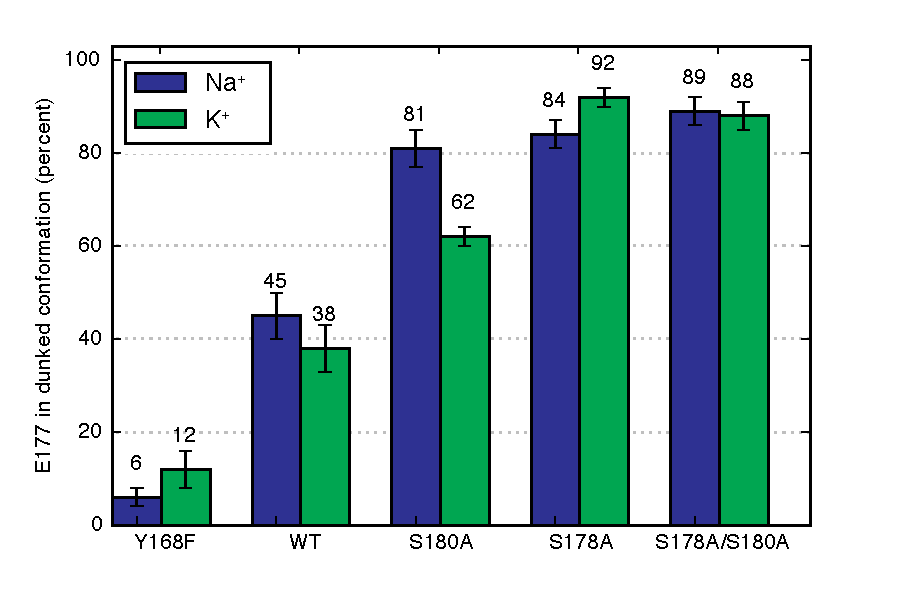
\includegraphics[width=0.5\textwidth]{nav6/Nav6Fig2}
\caption[E177 side chain conformational isomerization]{\textbf{E177 side chain conformational isomerization}. (\textbf{A}) The mean percentage of simulation time in the E177 side chain adopted a lumen-facing state. Data is shown for Y168F, WT, S180A, S178A, and S178A/S180A in the presence of either Na$^+$ (blue) or K$^+$ (green). Error bars are computed as the standard error of mean across all simulation repeats.}
\label{fig:nav6fig2}
\end{figure}

Conformational isomerization alters the free energy of ion conduction within the SF. We report the one-dimensional potential of mean force for Na$^+$ (Fig. \ref{fig:nav6fig3} A,C) and K$^+$ (Fig. \ref{fig:nav6fig3} B,D) movement along the pore axis for the WT model and all mutants studied. Although ionic conduction in Nav channels is a multi-ion process, by projecting the multi-dimensional free energy of ionic conduction onto the channel axis, we capture the essential differences in the multi-ion conduction process. The 1D PMF for Na$^+$ and K$^+$ in the WT model (Fig. \ref{fig:nav6fig3} A-B, black line) highlight the `E', `EL', and `LT' binding sites of the SF, broadly located at positions -4, 0, and 4 \AA, respectively. Differences in the 1D free energy profile for Na$^+$ and K$^+$ in the WT datasets result from a difference in the multi-ion conduction mechanism. A relatively minor difference exists between the free energy of ion conduction in the WT and S180A models (Fig. \ref{fig:nav6fig3} A-B), suggesting that while glutamic acid fluctuations have nearly doubled, ion binding is largely unperturbed and the diffusive energy landscape of the SF is preserved. In the S180A mutant, increased dunking resulted in an increase of SF occupancy by Na$^+$ from 2.1$\pm$0.1 to 2.6$\pm$0.1 ions compared to the WT model, stemming primarily from greater `EL' binding (\Cref{fig:nav6figS2,fig:nav6figS3}). In the S178A and S178A/S180A mutants, increased E177 dunking reduces binding at the `high-field strength' site (referred to as the `E' site in our work), which has the largest effect on K$^+$ binding. Although dunking was increased in the S178A and S178A/S180A models, the commensurate decrease of `E' binding resulted in no net change of SF occupancy by Na$^+$, again due to increased `EL' binding (\Cref{fig:nav6figS4,fig:nav6figS5}). In all three Ser-to-Ala mutants, increased E177 dunking reduces a small barrier within the SF between the `EL' and `LT' sites. The free energy of ion conduction in the Y168F mutant (Fig. \ref{fig:nav6fig3} C-D), having greatly reduced E177 conformational isomerization, results in a significant barrier between the `E' and `LT' states that permits rapid Na$^+$ diffusion, and to a lesser extent the conduction of K$^+$. We examined the 1D PMF for ion conduction in the limit of 0\% E177 dunking for the WT model, referred to as `E177 DR', and barrier for ion conduction was within error of the Y168F mutant. In both reduced dunking models, SF occupancy of Na$^+$ was decreased to 1.99$\pm$0.01 and 1.95$\pm$0.02 ions in Y168F and E177 DR, respectively, compared to 2.1$\pm$0.1 in the WT (Fig. \ref{fig:nav6figS6}). This suggests that the crystallographic state of the E177 in the SF can be effectively stabilized by the Y168F mutation. 

\begin{figure}[!ptb]
\centering
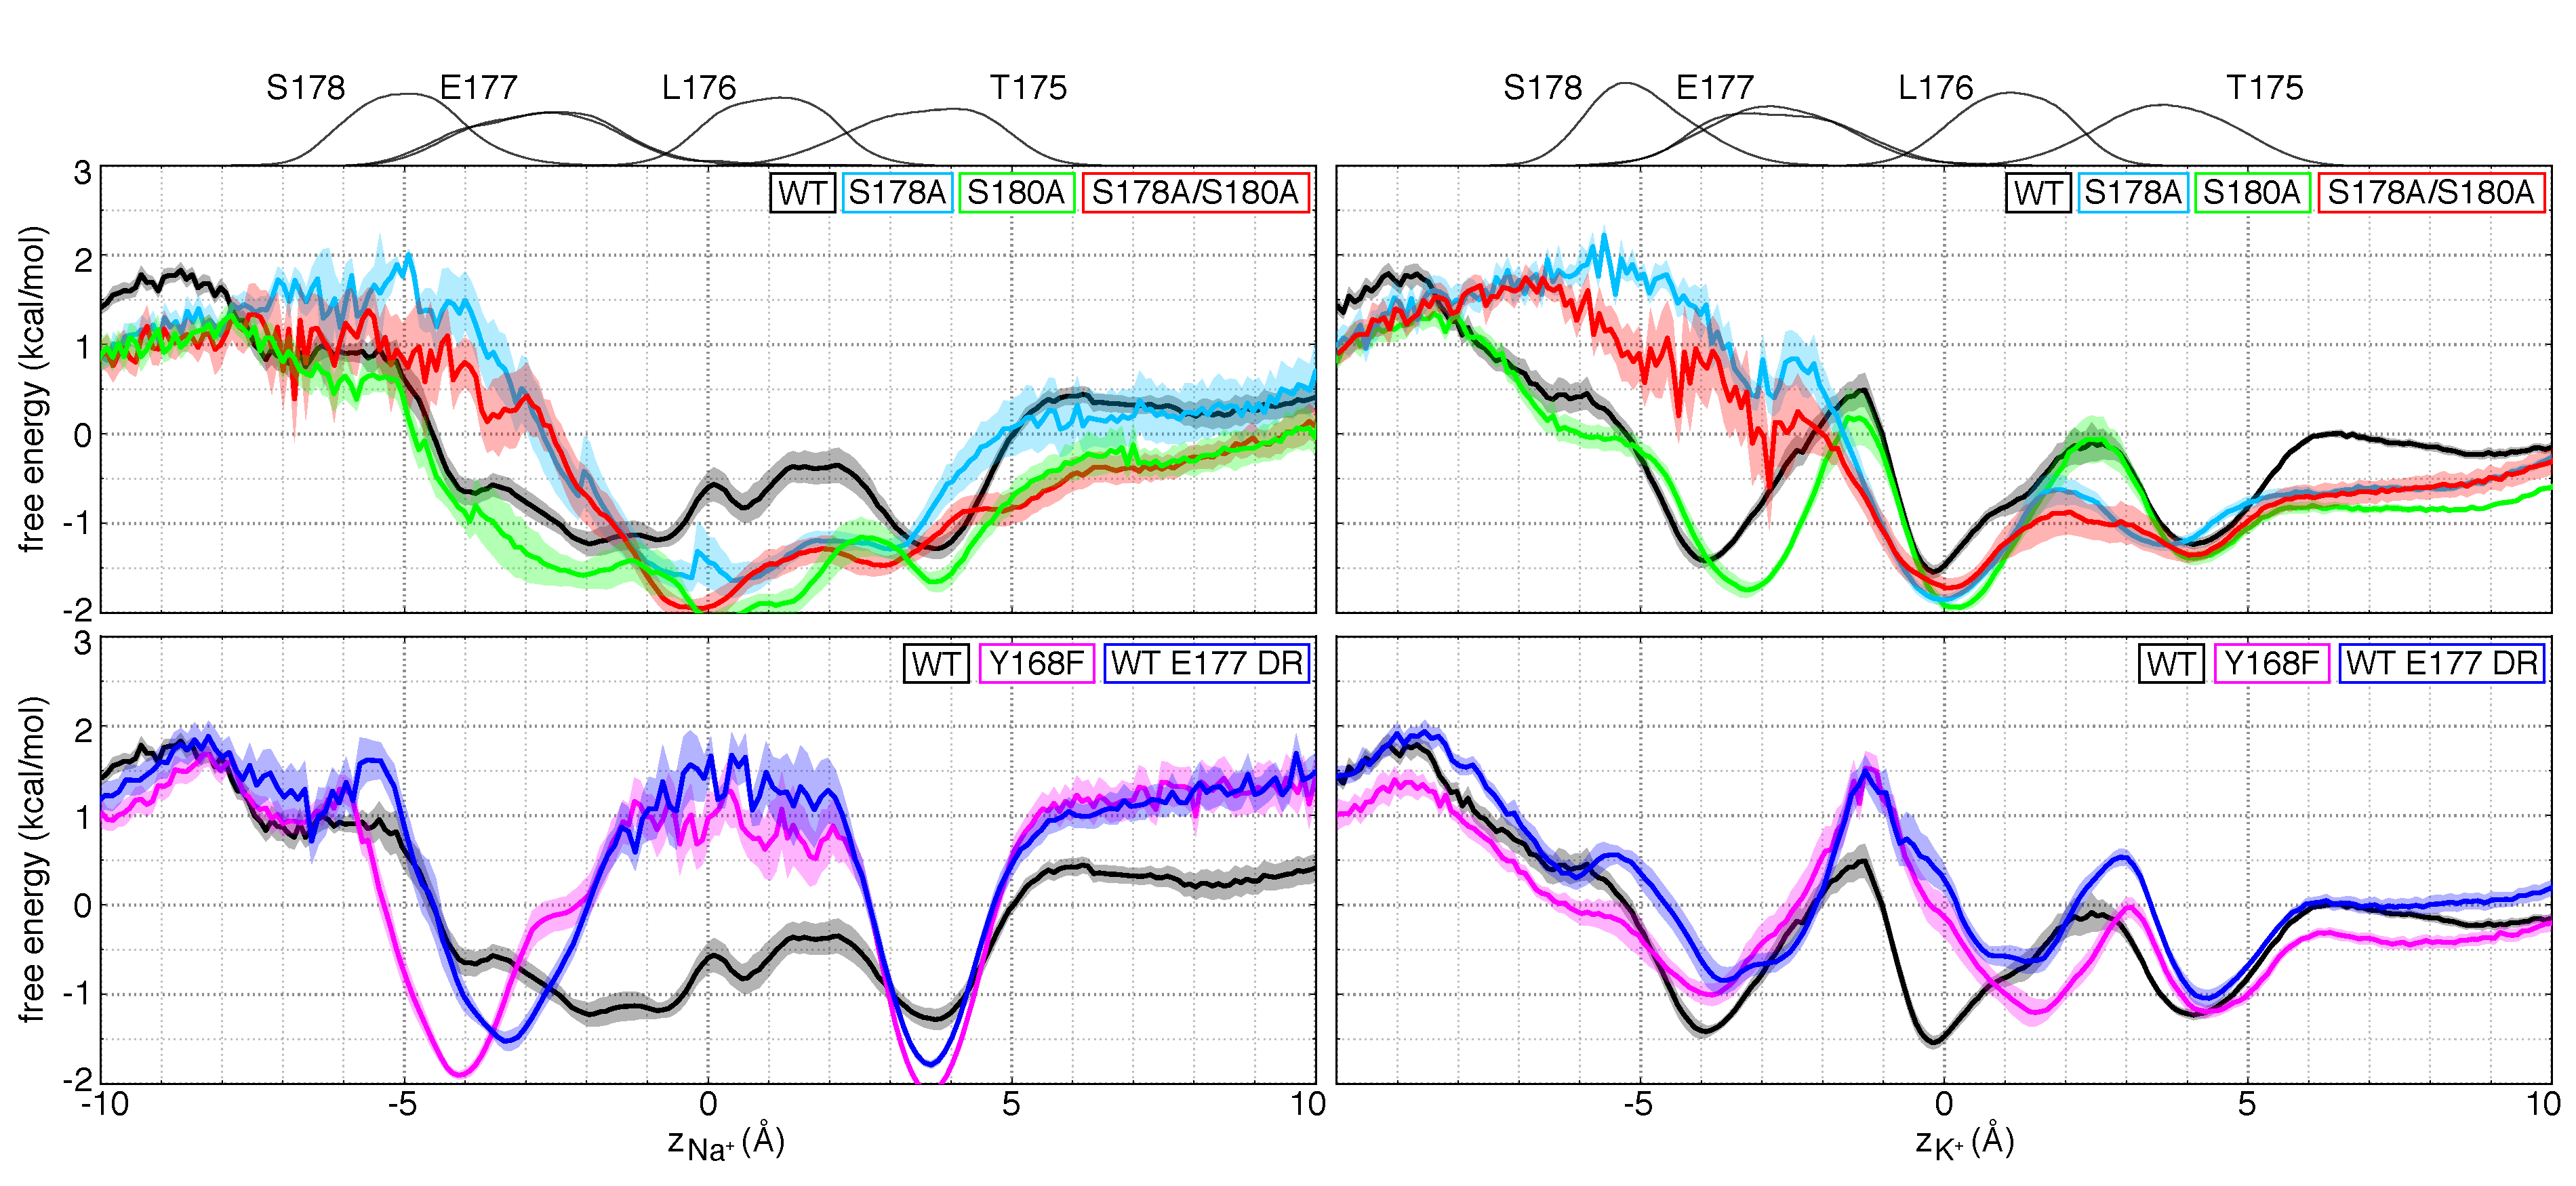
\includegraphics[width=0.9\textwidth]{nav6/Nav6Fig3}
\caption[Potential of mean-force (PMF) for the movement of Na$^+$ and K$^+$ along the channel axis]{\textbf{Potential of mean-force (PMF) for the movement of Na$^+$ and K$^+$ along the channel axis}. (\textbf{A}) One-dimensional multi-ion PMFs for pure Na$^+$ (left column) or K$^+$ (right column) movement along the channel axis in the (A-B) WT, S178A, S180A, S178A/S180A models. One-dimensional PMFs are also shown for the (C-D) WT, Y168F, and WT model with E177 dihedral restraints (E177 DR). The reference state (zero free energy) is defined as the bulk extracellular value for Na$^+$ or K$^+$ in each dataset separately. The axial distribution of pore-lining oxygen atoms of S178, E177, L176, and T175 are shown from WT simulations above both Na$^+$ and K$^+$ plots.}
\label{fig:nav6fig3}
\end{figure}

In an alternate forcefield with higher channel occupancy ($\sim 2.6$ using OPLS compared to $\sim 2.2$ using CHARMM), simulations of S178A, S180A, S178A/S180A, and Y168F were recomputed. A linear relationship between the aforementioned mutations and the degree of conformational isomerization of E177 was observed for simulations with Na$^+$ (Fig. \ref{fig:nav6figS1} A), although the perturbation induced by the Y168F mutation was far less dramatic (44$\pm$3\% in OPLS compared to 6$\pm$2\% in CHARMM). Simulations of these mutants performed in the absence of bulk ions reveal that native channel fluctuations may be perturbed, even though low ion conditions are unlikely to occur in the physiological state of the channel. For example, in the absence of salt, Glu adopted a dunked conformation in 5$\pm$2 frames for WT, compared to 33$\pm$2 frames for S178A. However, these mutations did not directly translate into differences in the 1D PMF for Na$^+$ (Fig. \ref{fig:nav6figS1} B), suggesting that our mechanisms may be sensitive to force field parameterization. Additional experimental validation must be performed in order to confirm the effect of conformational isomerization of Glu sidechains on ionic conductance.

\begin{figure}[!ptb]
\centering
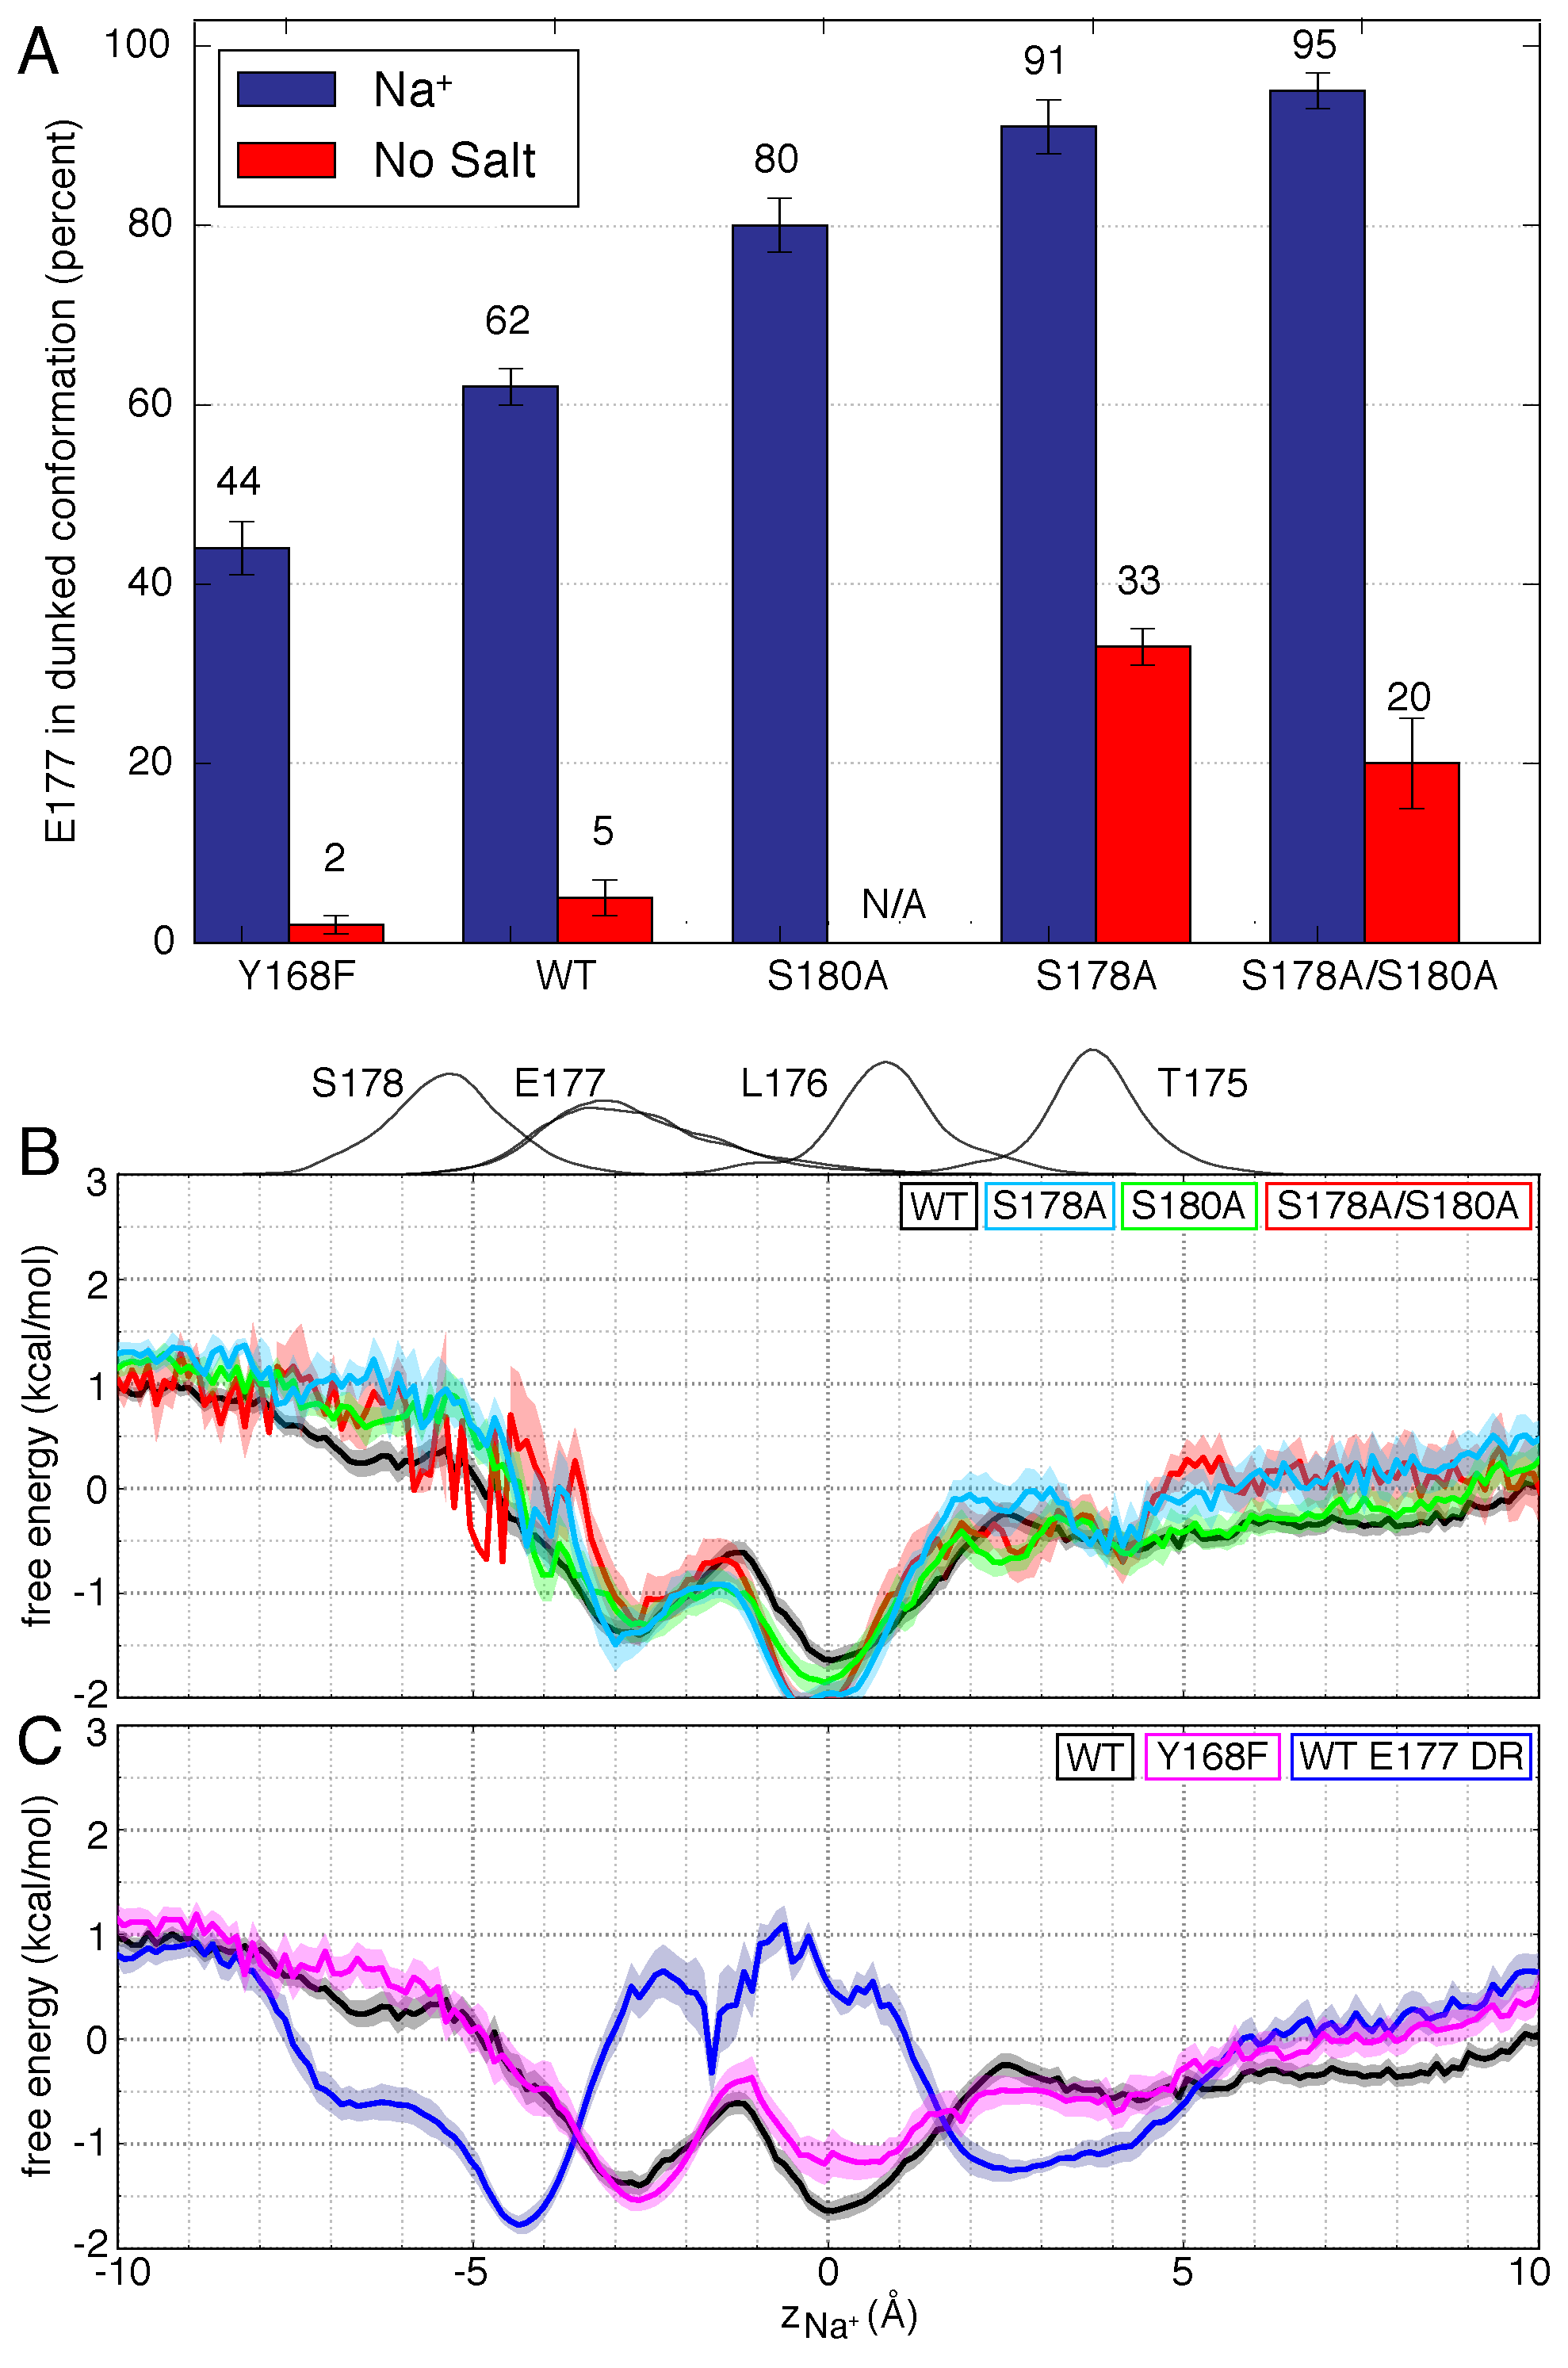
\includegraphics[width=0.7\textwidth]{nav6/Nav6FigS1}
\caption[E177 side chain conformational isomerization and PMF for the movement of Na$^+$ with the OPLS force field]{\textbf{E177 side chain conformational isomerization and PMF for the movement of Na$^+$ with the OPLS force field}. (\textbf{A}) The mean percentage of simulation time in the E177 side chain adopted a lumen-facing state. Data is shown for Y168F, WT, S180A, S178A, and S178A/S180A in the presence of either Na$^+$ (blue) or no ions (red). Error bars are computed as the standard error of mean across all simulation repeats. One-dimensional multi-ion PMFs for Na$^+$ movement along the channel axis in the (\textbf{B}) WT, S178A, S180A, S178A/S180A models. One-dimensional PMFs are also shown for the (\textbf{C}) WT, Y168F, and WT model with E177 dihedral restraints (E177 DR). The reference state (zero free energy) is defined as the bulk extracellular value for Na$^+$ in each dataset separately. The axial distribution of pore-lining oxygen atoms of S178, E177, L176, and T175 are shown from WT simulations above both Na$^+$ and K$^+$ plots.}
\label{fig:nav6figS1}
\end{figure}

We examined the relationship between E177 fluctuations and the multi-ion conduction mechanism using 2D PMFs for distinct ion pairs in the 2 and 3 ion occupancy states (\Cref{fig:nav6figS2,fig:nav6figS3,fig:nav6figS4,fig:nav6figS5,fig:nav6figS6}). This analysis provides information about the preferred positions of ion pairs and greater detail regarding the origin of features in the 1D PMF. With respect to the WT model, the S180A model has a reduced free energy barrier at the site within the SF where ions bind predominately to S178 and E177 with. This axial position corresponds to the location where multiple Na$^+$ have been observed to bind at same axial position (\Cref{fig:nav6figS2,fig:nav6figS3}). The free energy landscape for Na$^+$ is more diffusive for individual ions in the 3 ion state than the 2 ion state, but increased dunking in this mutant does not enhance this effect compared to the WT system. The Na$^+$ free energy surface is flatter than that of K$^+$ throughout the SF, which is common to both S180A and WT models. Increased E177 conformational isomerization in the S180A model appears to have no significant effect on the conduction mechanism within the SF. 

\begin{figure}[!ptb]
\centering
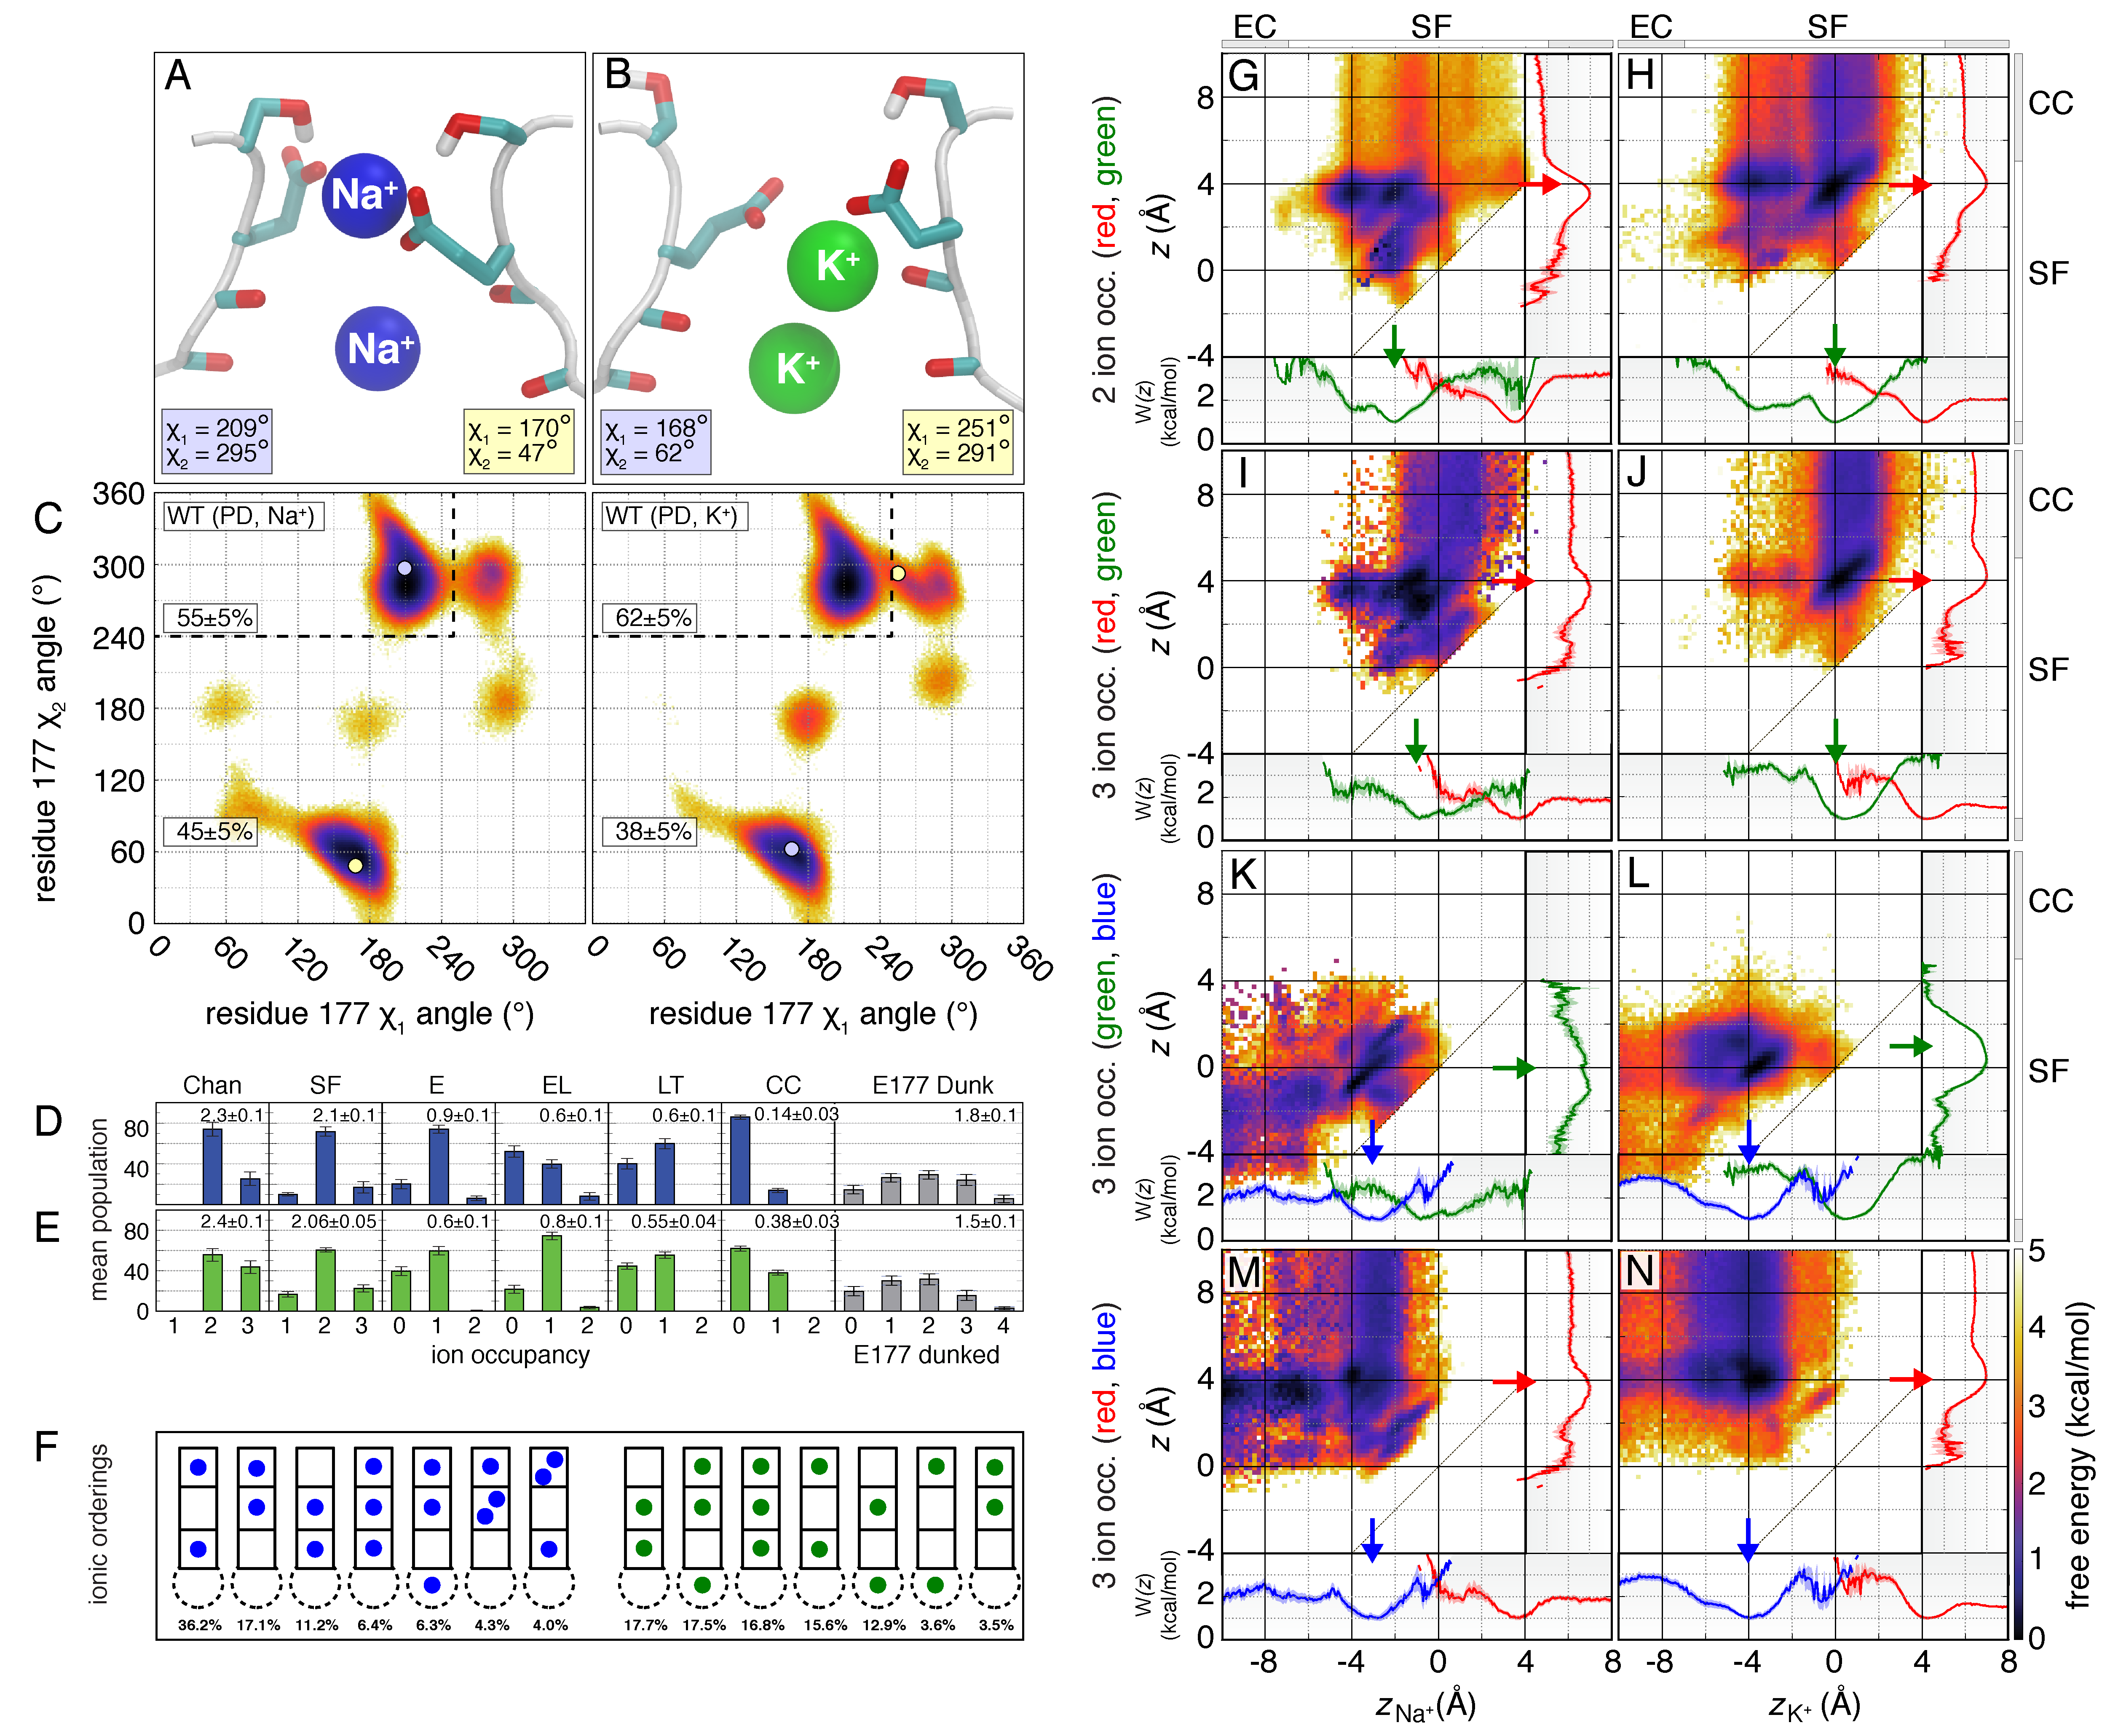
\includegraphics[width=0.8\textwidth]{nav6/Nav6FigS2}
\caption[Binding statistics and potential of mean-force (PMF) for the movement of Na$^+$ and K$^+$ along the channel axis in the WT PD model]{\textbf{Binding statistics and potential of mean-force (PMF) for the movement of Na$^+$ and K$^+$ along the channel axis in the WT PD model}. (\textbf{A-B}) Representative snapshots of the SF for high population ionic configurations in the presence of Na$^+$ and K$^+$, with E177 sidechain $\chi_1$ and $\chi_2$ angles shown for both left (purple) and right (yellow) subunits. (\textbf{B}) Population of E177 side chain torsions ($\chi_1$, $\chi_2$) across all WT simulation data for Na$^+$ and K$^+$. ($\chi_1$, $\chi_2$) pairs are shown as yellow and purple dots in correspondence with the left and right subunits in (A-B), respectively. A dashed line separates the crystallographic E177 side chain configuration and the lumen-facing conformation, with total state populations shown within each region. Ionic occupancy of the entire channel and SF, as well as specific `E', `EL', `LT', and `CC' binding sites, as well as the distribution of number of dunked E177 side chains, for (\textbf{D}) Na$^+$ and (\textbf{E}) K$^+$. (\textbf{F}) The seven highest population ionic configurations with the channel for Na$^+$ and K$^+$, where the four primary binding sites are identified as `E', `EL', `LT', and `CC' from top to bottom. Two-dimensional potential of mean-force (PMF) for (\textbf{G, I, K, M}) Na$^+$ and (\textbf{H, J, L, N}) K$^+$ pairs along the channel axis. Ions are ranked by axial position from CC to EC with the colors `red', `green', and `blue' for both ion types. PMFs for Na$^+$ and K$^+$ are computed between ion pairs for channel occupancy states; (\textbf{G,H}) 2 and (\textbf{I-N}) 3. For three ion occupancy, all distinct two ion pairs are plotted. On all 2D PMFs a one-dimensional projection of the axial free energy for each ion are shown on the vertical and horizontal axes and are colored for the target ion (identified with colored arrows). The reference state (zero free energy) of each panel is set to the highest probability microstate within each channel occupancy state sub-ensemble, which applies to all subsequent ion pair 2D PMFs.}
\label{fig:nav6figS2}
\end{figure}

\begin{figure}[!ptb]
\centering
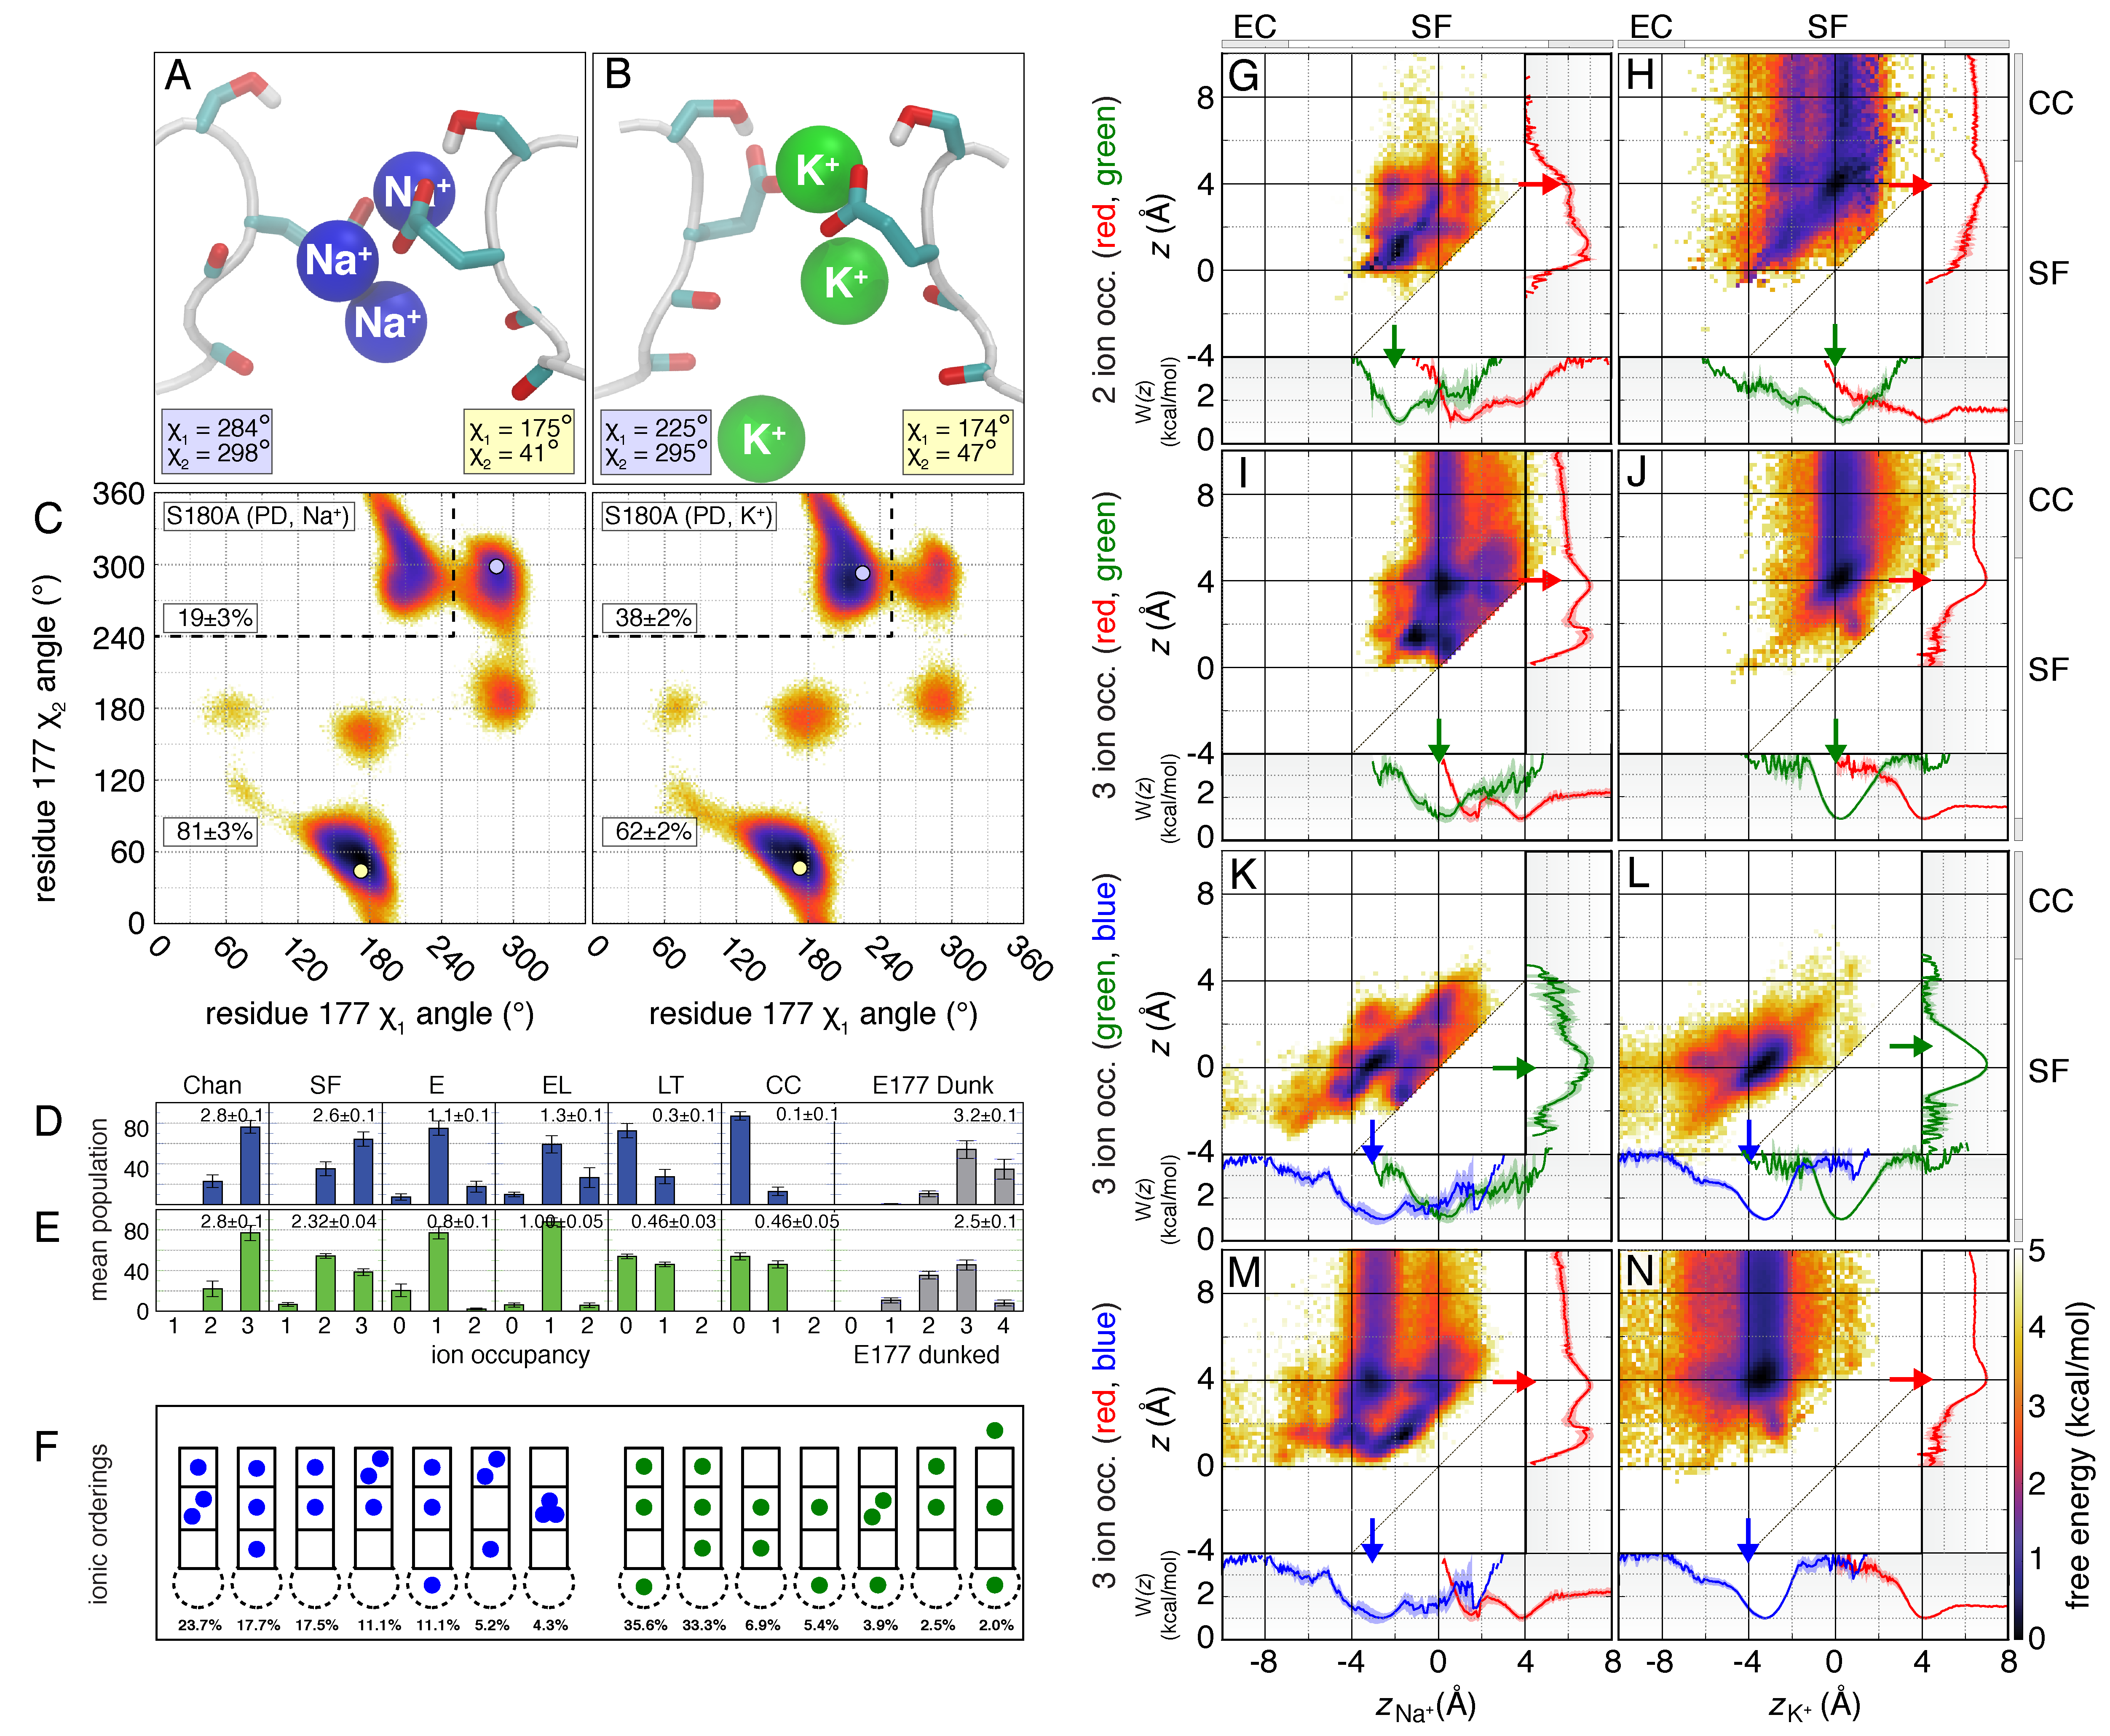
\includegraphics[width=0.8\textwidth]{nav6/Nav6FigS3}
\caption[Binding statistics and potential of mean-force (PMF) for the movement of Na$^+$ and K$^+$ along the channel axis in the S180A PD model]{ \textbf{Binding statistics and potential of mean-force (PMF) for the movement of Na$^+$ and K$^+$ along the channel axis in the S180A PD model}. (\textbf{A-B}) Representative snapshots of the SF for high population ionic configurations in the presence of Na$^+$ and K$^+$. (\textbf{C}) Population of E177 side chain torsions ($\chi_1$, $\chi_2$) across all S180A simulation data for Na$^+$ and K$^+$. Ionic occupancy of the entire channel and SF, as well as specific `E', `EL', `LT', and `CC' binding sites, as well as the distribution of number of dunked E177 side chains, for (\textbf{D}) Na$^+$ and (\textbf{E}) K$^+$. (\textbf{F}) The seven highest population ionic configurations with the channel for Na$^+$ and K$^+$, where the four primary binding sites are identified as `E', `EL', `LT', and `CC' from top to bottom. Two-dimensional potential of mean-force (PMF) for (\textbf{G, I, K, M}) Na$^+$ and (\textbf{H, J, L, N}) K$^+$ pairs along the channel axis. PMFs for Na$^+$ and K$^+$ are computed between ion pairs for channel occupancy states; (\textbf{G, H}) 2 and (\textbf{I-N}) 3. For three ion occupancy, all distinct two ion pairs are plotted. For more information, refer to the caption of Figure \ref{fig:nav6figS2}.}
\label{fig:nav6figS3}
\end{figure}

In the S178A and S178A/S180A models, concerted motion of ion pairs appears reduced in both 2 and 3 ion occupancy states due to reduced binding at the `E' site at $\approx$-4 \AA (\Cref{fig:nav6figS4,fig:nav6figS5}). However, in both ion occupancy states, dual occupancy of the `E' binding site by Na$^+$ and K$^+$ is increased relative to the WT channel, suggesting that the molecular mechanism of conduction is perturbed. As a result of this change in the outer binding site of the SF, Na$^+$ and K$^+$ bind in similar ways within the SF, having outer and central ion binding sites shifted to the intracellular side of the SF compared to the WT model. These Ser-to-Ala models have a higher propensity for Na$^+$ and K$^+$ binding at the same axial position compared to the WT model. The free energy barrier for K$^+$ at position $\approx -2$ \AA is not strongly present in S178A and S178A/S180A models, suggesting that Na$^+$ selectivity is impaired. 

\begin{figure}[!ptb]
\centering
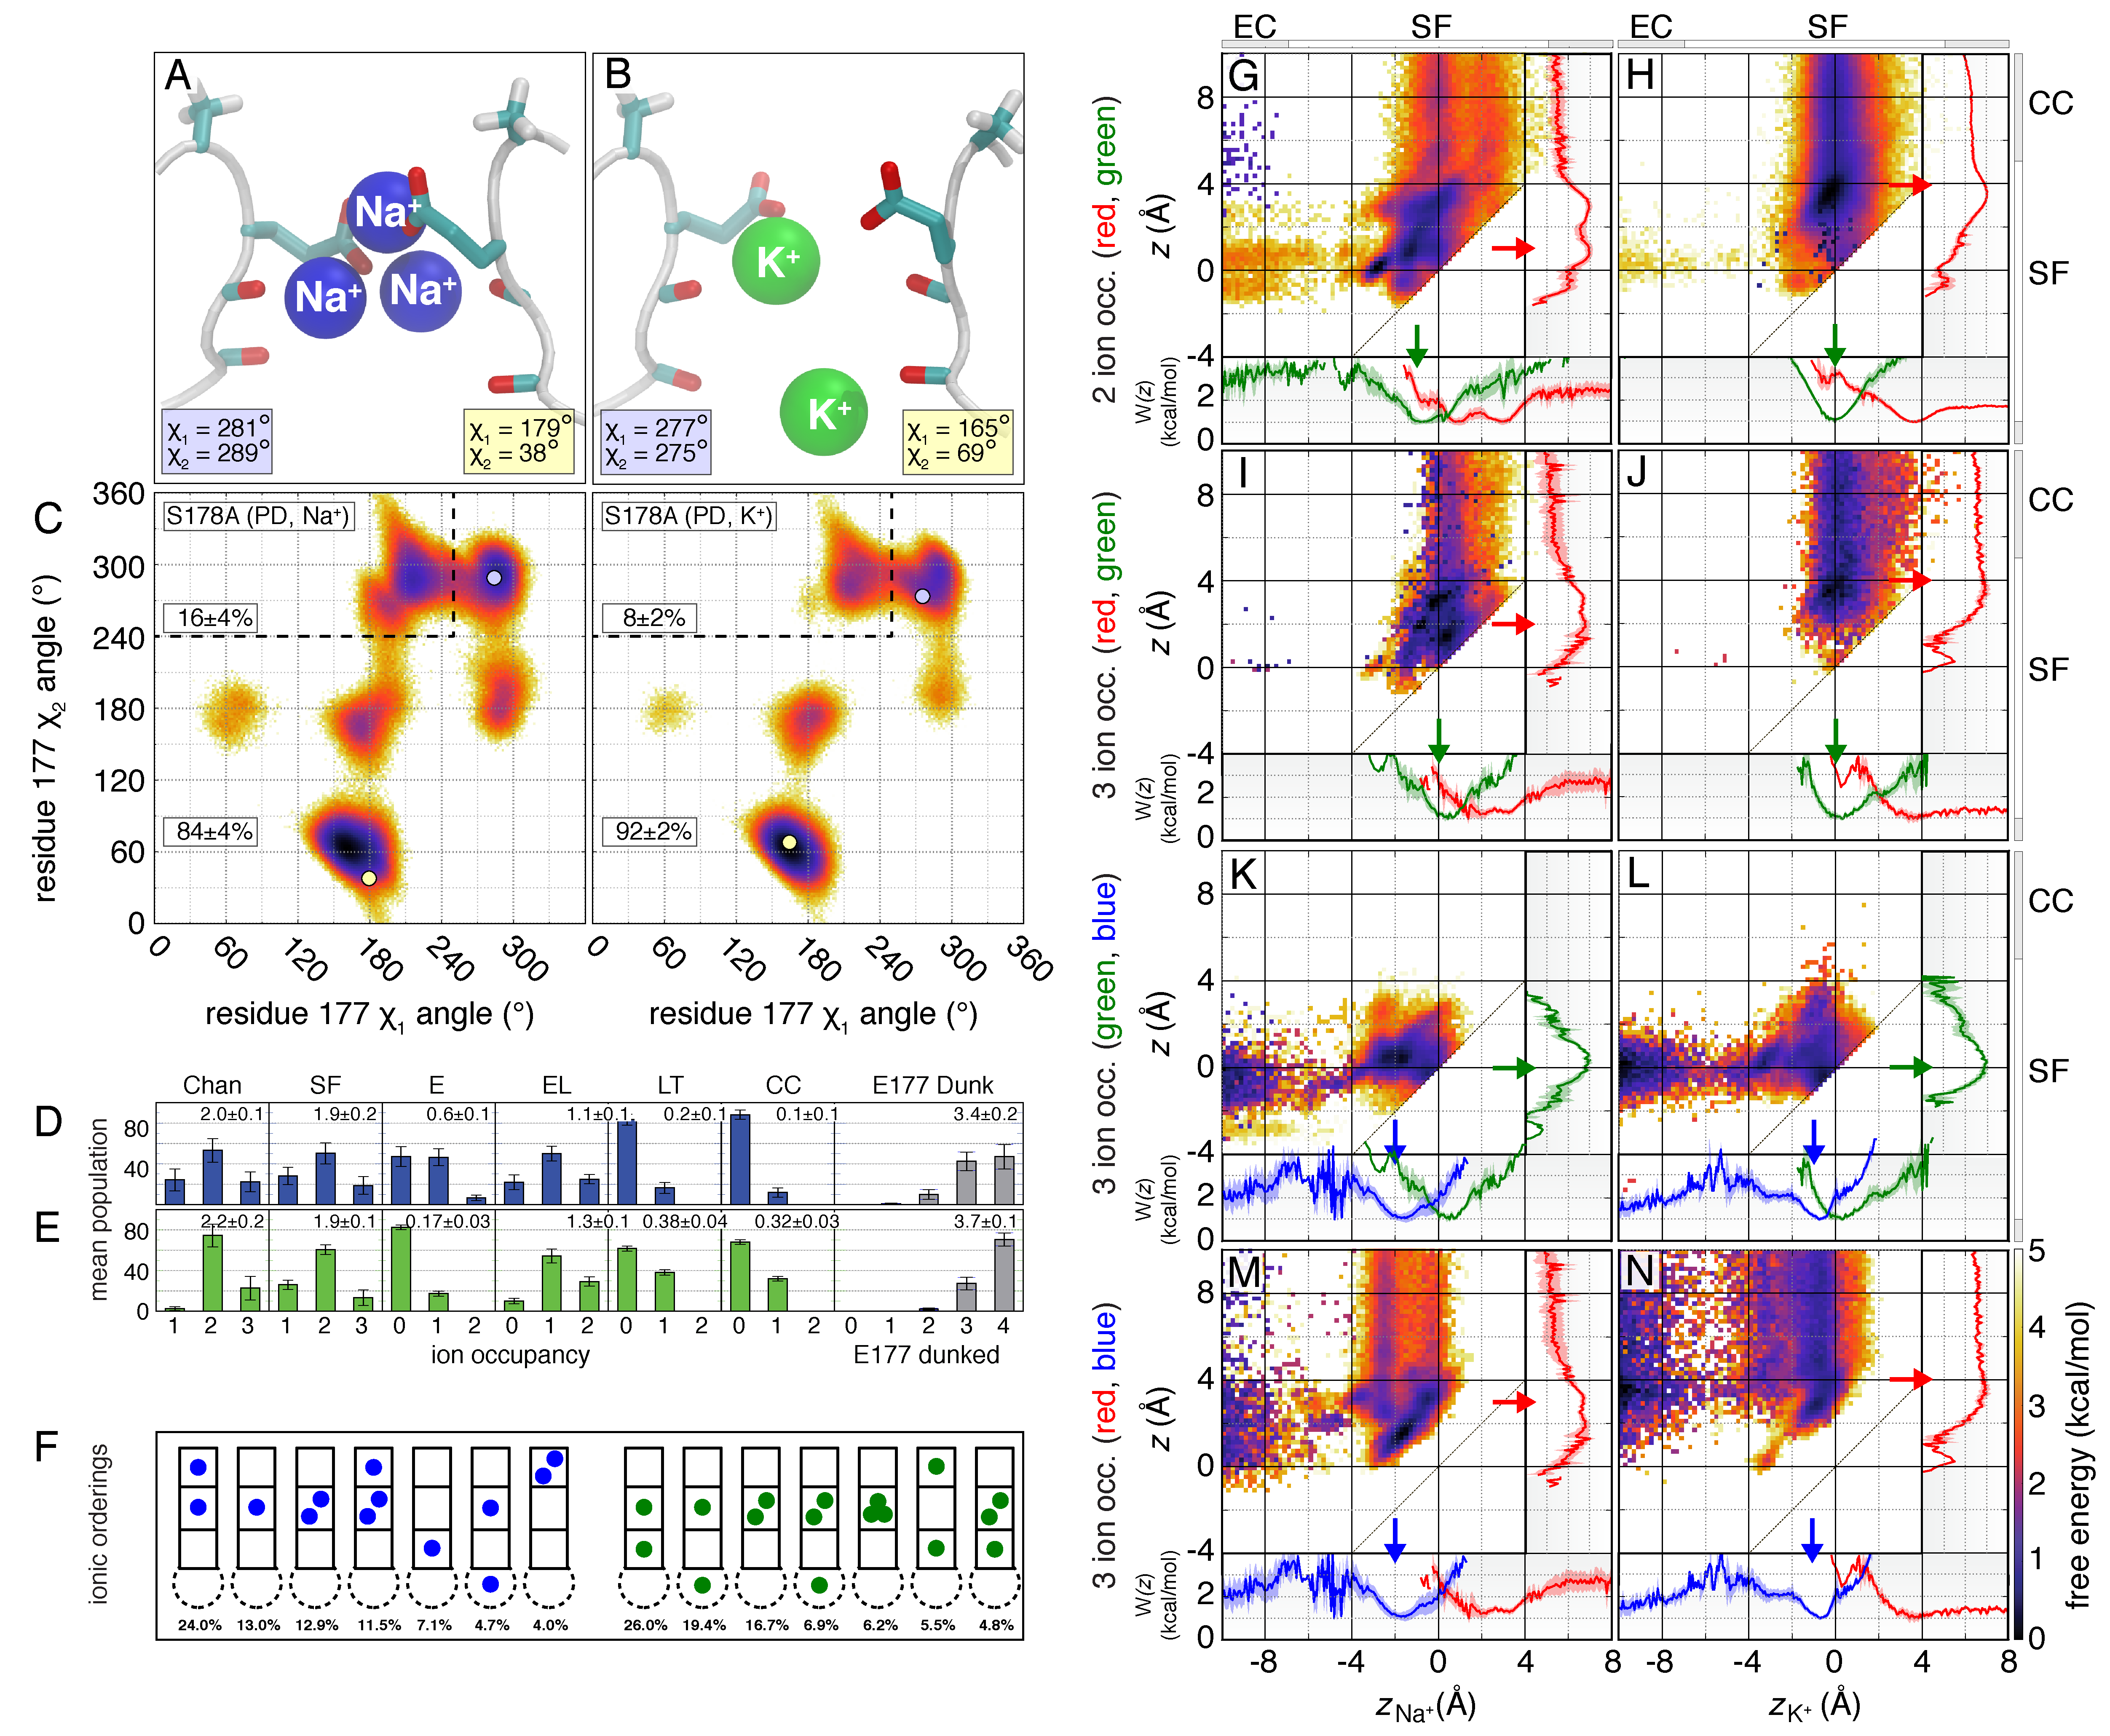
\includegraphics[width=0.8\textwidth]{nav6/Nav6FigS4}
\caption[Binding statistics and potential of mean-force (PMF) for the movement of Na$^+$ and K$^+$ along the channel axis in the S178A PD model]{ \textbf{Binding statistics and potential of mean-force (PMF) for the movement of Na$^+$ and K$^+$ along the channel axis in the S178A PD model}. (\textbf{A-B}) Representative snapshots of the SF for high population ionic configurations in the presence of Na$^+$ and K$^+$. (\textbf{C}) Population of E177 side chain torsions ($\chi_1$, $\chi_2$) across all S178A simulation data for Na$^+$ and K$^+$. Ionic occupancy of the entire channel and SF, as well as specific `E', `EL', `LT', and `CC' binding sites, as well as the distribution of number of dunked E177 side chains, for (\textbf{D}) Na$^+$ and (\textbf{E}) K$^+$. (\textbf{F}) The seven highest population ionic configurations with the channel for Na$^+$ and K$^+$, where the four primary binding sites are identified as `E', `EL', `LT', and `CC' from top to bottom. Two-dimensional potential of mean-force (PMF) for (\textbf{G, I, K, M}) Na$^+$ and (\textbf{H, J, L, N}) K$^+$ pairs along the channel axis. PMFs for Na$^+$ and K$^+$ are computed between ion pairs for channel occupancy states; (\textbf{G, H}) 2 and (\textbf{I-N}) 3. For three ion occupancy, all distinct two ion pairs are plotted. For more information, refer to the caption of Figure \ref{fig:nav6figS2}.}
\label{fig:nav6figS4}
\end{figure}

\begin{figure}[!ptb]
\centering
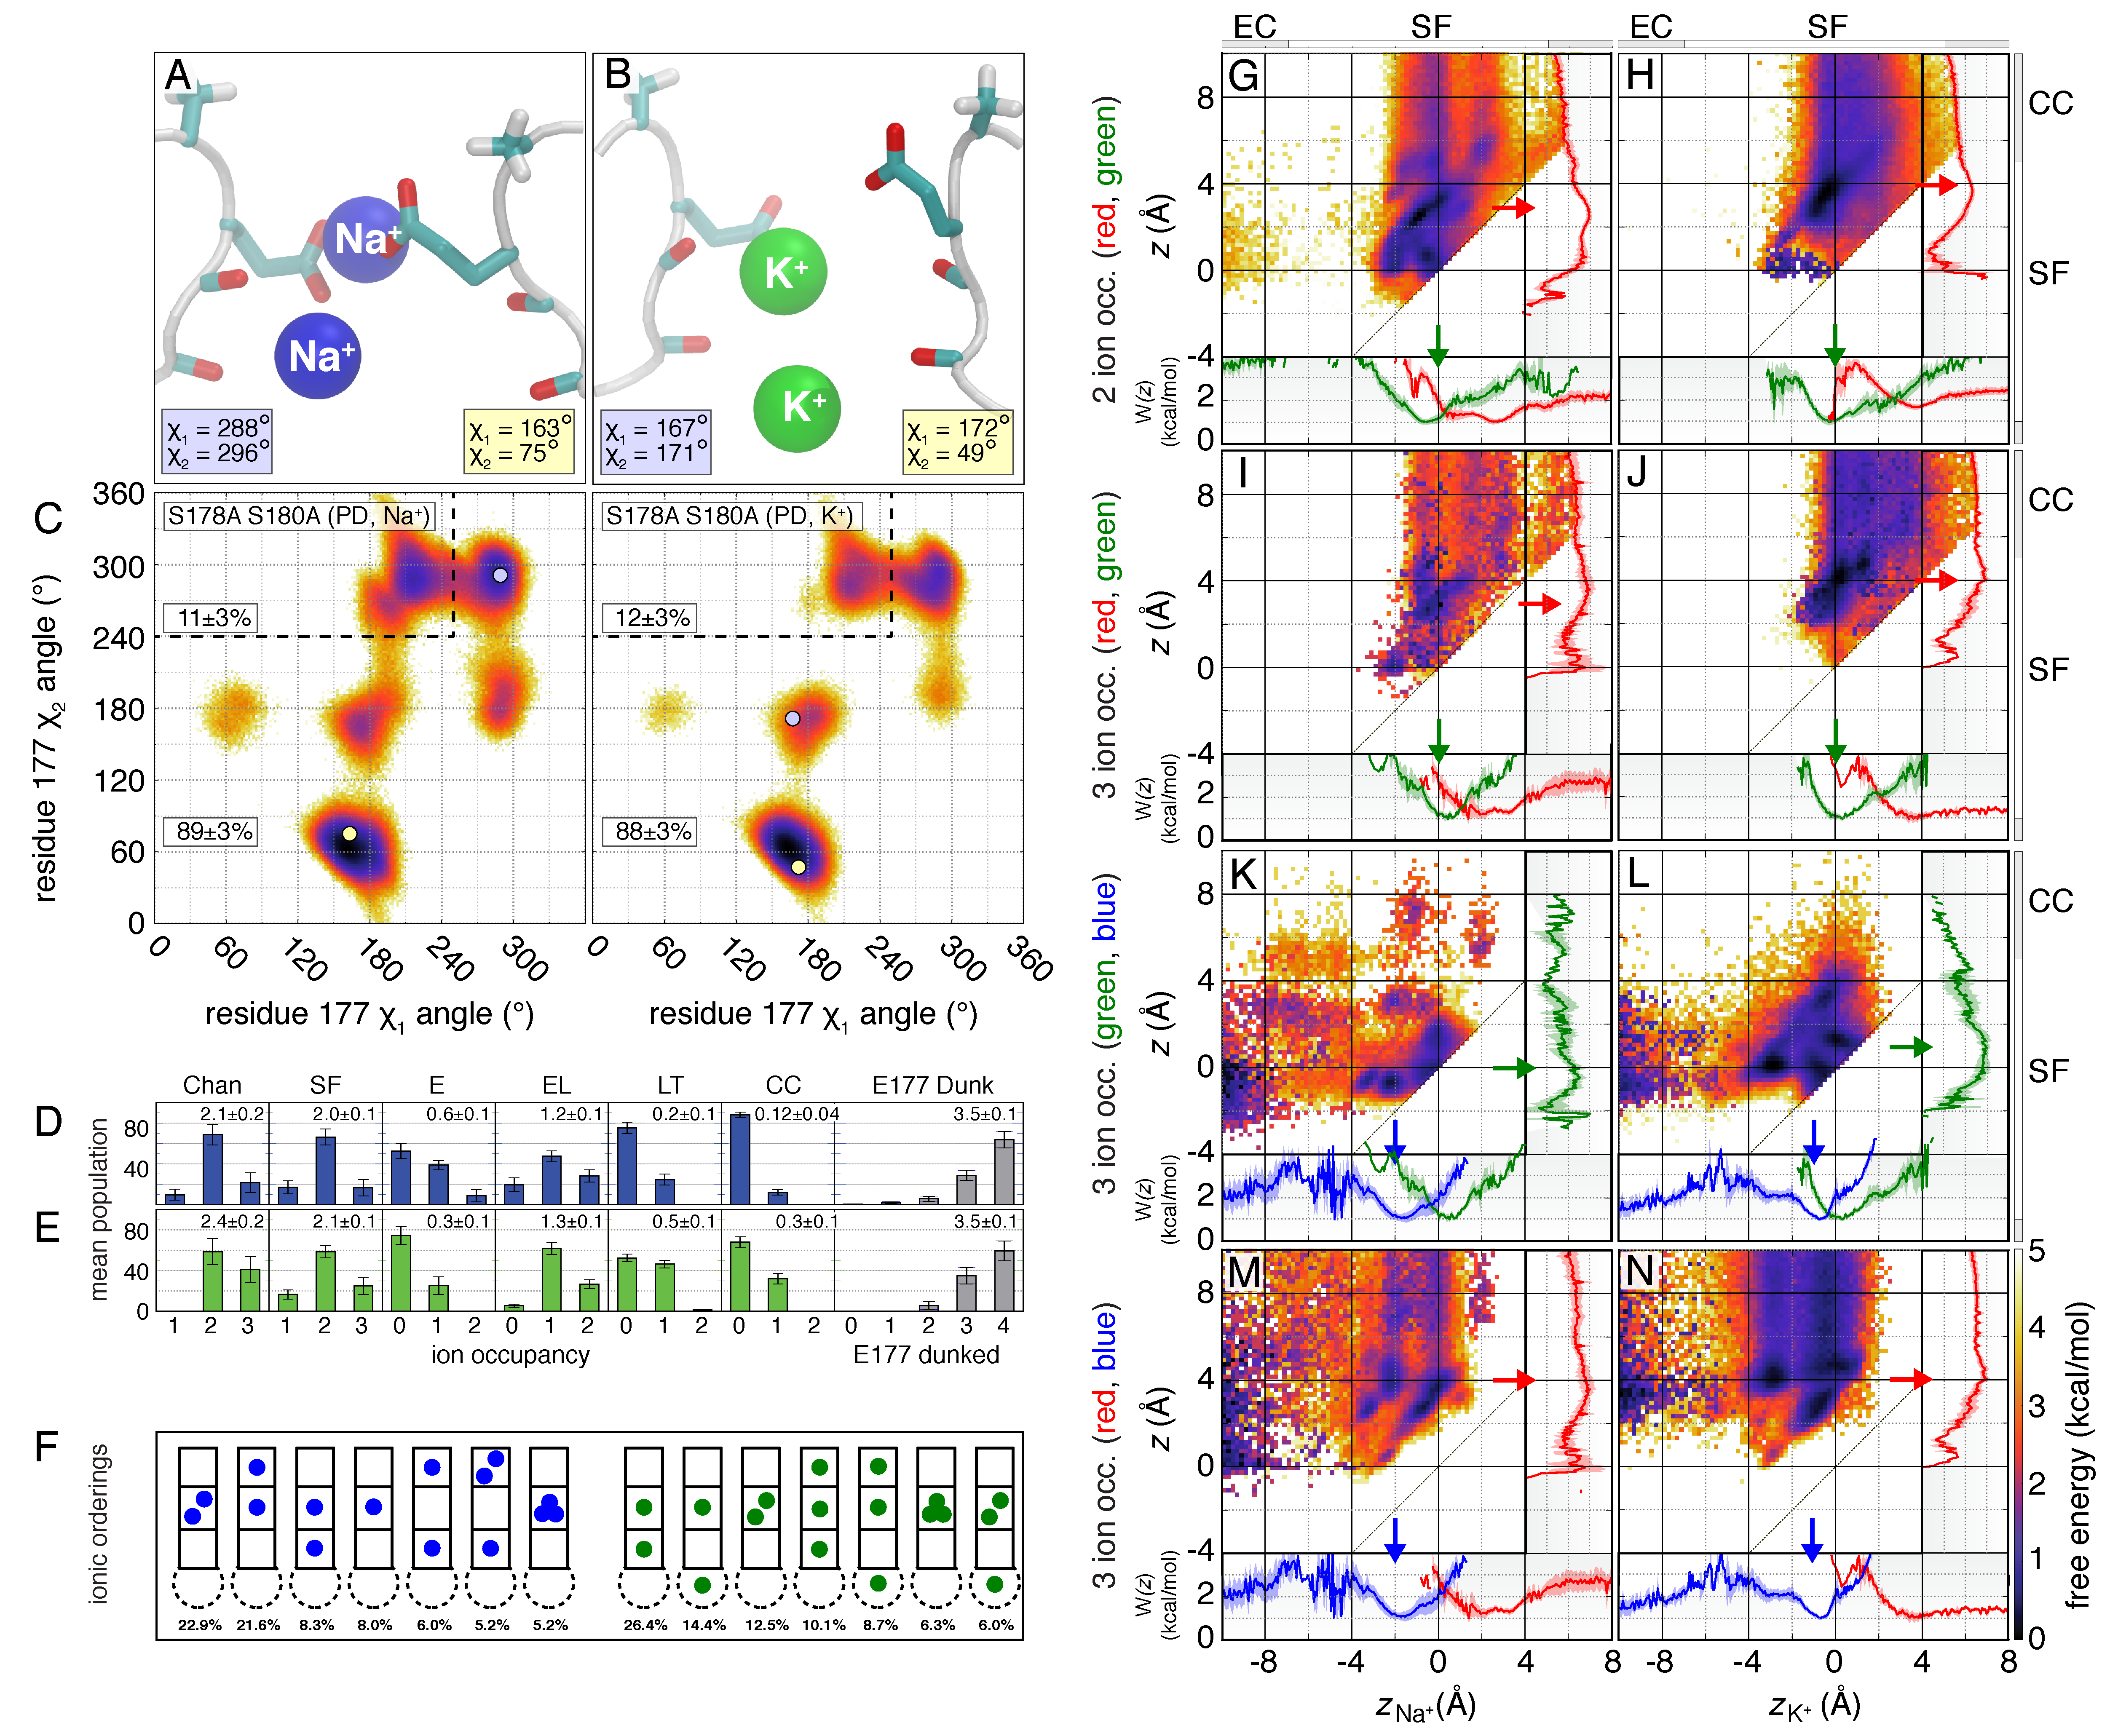
\includegraphics[width=0.8\textwidth]{nav6/Nav6FigS5}
\caption[Binding statistics and potential of mean-force (PMF) for the movement of Na$^+$ and K$^+$ along the channel axis in the S178A/S180A PD model]{ \textbf{Binding statistics and potential of mean-force (PMF) for the movement of Na$^+$ and K$^+$ along the channel axis in the S178A/S180A PD model}. (\textbf{A-B}) Representative snapshots of the SF for high population ionic configurations in the presence of Na$^+$ and K$^+$. (\textbf{C}) Population of E177 side chain torsions ($\chi_1$, $\chi_2$) across all S178A/S180A simulation data for Na$^+$ and K$^+$. Ionic occupancy of the entire channel and SF, as well as specific `E', `EL', `LT', and `CC' binding sites, as well as the distribution of number of dunked E177 side chains, for (\textbf{D}) Na$^+$ and (\textbf{E}) K$^+$. (\textbf{F}) The seven highest population ionic configurations with the channel for Na$^+$ and K$^+$, where the four primary binding sites are identified as `E', `EL', `LT', and `CC' from top to bottom. Two-dimensional potential of mean-force (PMF) for (\textbf{G, I, K, M}) Na$^+$ and (\textbf{H, J, L, N}) K$^+$ pairs along the channel axis. PMFs for Na$^+$ and K$^+$ are computed between ion pairs for channel occupancy states; (\textbf{G, H}) 2 and (\textbf{I-N}) 3. For three ion occupancy, all distinct two ion pairs are plotted. For more information, refer to the caption of Figure \ref{fig:nav6figS2}.}
\label{fig:nav6figS5}
\end{figure}

In the dunking reduced Y168F model, there is a dramatic alteration of Na$^+$ binding and mobility. Na$^+$ and K$^+$ preferentially adopt a single-file 2 ion state at `E' and `LT' sites (Fig. \ref{fig:nav6figS6}). In both cases Na$^+$ rarely adopts the `LT' site, but K$^+$ is capable of doing so along with a higher likelihood of concerted motion. Based on these results, we would expect that Na$^+$ selectivity is also impaired or potentially reversed in favour of K$^+$. The concerted and knock-on conduction mechanisms are significantly disrupted for Na$^+$ in this model, and are nearly identical to the E177 DR system. Together, these results provide a foundation for experimental validation of the role of channel fluctuations in conduction and selectivity in Nav channels.

\begin{figure}[!ptb]
\centering
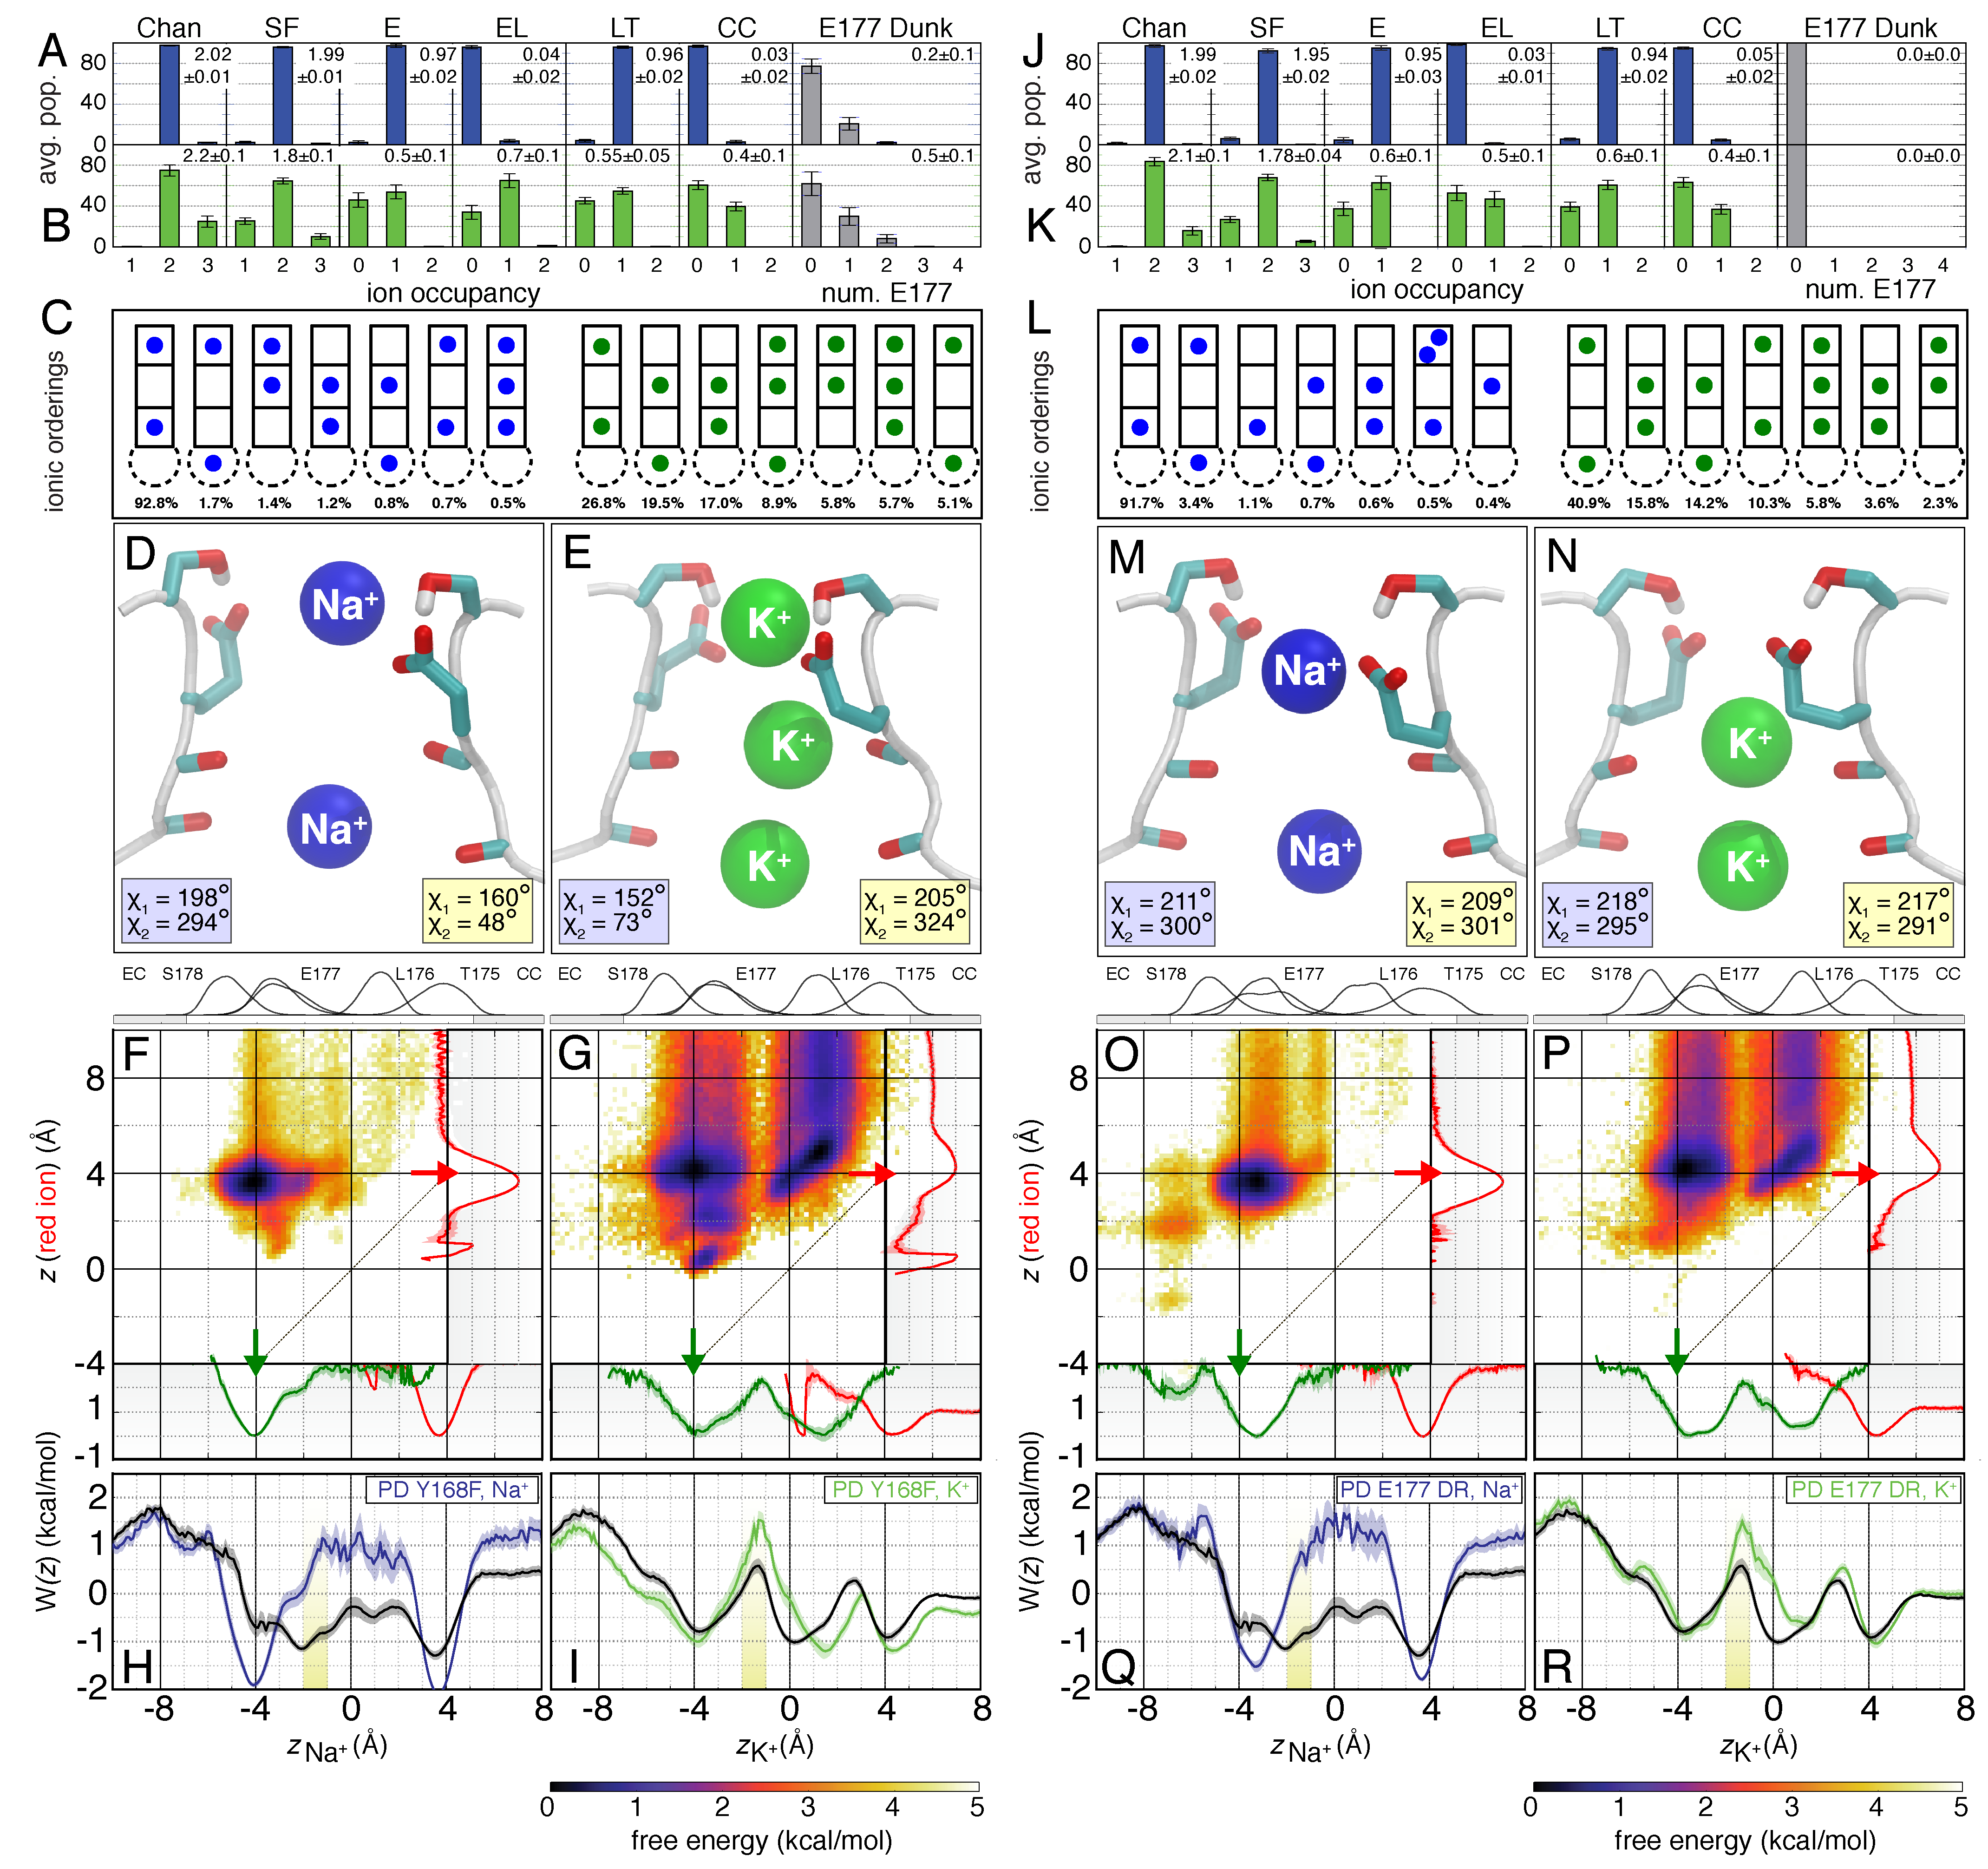
\includegraphics[width=0.8\textwidth]{nav6/Nav6FigS6}
\caption[Binding statistics and potential of mean-force (PMF) for the movement of Na$^+$ and K$^+$ along the channel axis in the Y168F and E177DR PD model]{ \textbf{Binding statistics and potential of mean-force (PMF) for the movement of Na$^+$ and K$^+$ along the channel axis in the Y168F and E177DR PD model}. Ionic occupancy of the entire channel and SF, as well as specific `E', `EL', `LT', and `CC' binding sites, as well as the distribution of number of dunked E177 side chains, for (\textbf{A}) Na$^+$ and (\textbf{B}) K$^+$. (\textbf{C}) The seven highest population ionic configurations with the channel for Na$^+$ and K$^+$, where the four primary binding sites are identified as `E', `EL', `LT', and `CC' from top to bottom. (\textbf{D-E}) Representative snapshots of the SF for high population ionic configurations in the presence of Na$^+$ and K$^+$. Two-dimensional potential of mean-force (PMF) for (\textbf{F}) Na$^+$ and (\textbf{G}) K$^+$ pairs along the channel axis for the two ion occupancy state. The multi-ion 1D PMF for (\textbf{H}) Na$^+$ and (\textbf{I}) K$^+$ movement is shown for the Y168F model (blue/green colored lines) as well as the WT model (black line) for reference. Identical plots are shown for the E177 dihedral restrained model (\textbf{J-R}).For more information, refer to the caption of Figure \ref{fig:nav6figS2}.}
\label{fig:nav6figS6}
\end{figure}

\section{Discussion}
Previous molecular simulations suggest that conformational isomerization of glutamic acid side chains in the SF of bacterial voltage-gated sodium channels plays a dual role of catalyzing Na$^+$ conduction and imparting Na$^+$ over K$^+$ selectivity (Chapters 4-5, \cite{Chakrabarti:2013kd}). Here we extend these findings by presenting a set of single-point mutations that displace the conformational equilibrium of E177. The propensity of E177 dunking was linked to quantitative changes in the free-energy of Na$^+$ and K$^+$ conduction. In the S180A mutant, Na$^+$ movement was made more diffusive through the SF, while K$^+$ movement was unaffected. In the S178A and S178A/S180A models, the free energy of Na$^+$ and K$^+$ conduction was similar. Lastly, in the Y168F mutant, Na$^+$ conduction through the SF was blocked, while free energy barriers for K$^+$ increased, but were still surmountable.

These results provide the basis for electrophysiological validation of the hypothesis that E177 dunking is fundamental to conduction and selectivity. Differences in the multi-ion conduction mechanism for Na$^+$ and K$^+$ with respect to the WT channel are expected to result in perturbations to single-channel conductance and electrophysiological measurements of selectivity. Quantitative estimates of conductance and selectivity in voltage-gated cation channels are challenging to compute using molecular simulations \cite{Jensen:2013gn}, and cannot be reliably computed in a closed-channel model, but nonetheless, our results lead to specific predictions. In broad terms, we hypothesize that increased dunking by means of mutations like S180A will increase Na$^+$ conductance and, conversely, decreased dunking by means of the Y168F mutation should decrease conductance. Our confidence in this relationship is stronger for the Y to F mutation, which has a dramatic effect on the dunking propensity and free energy of ion conduction. Based on our previous studies of competitive ion binding in relation to pure cation simulations in a closed-channel model, we hypothesize that the S180A mutant is more Na$^+$ selective and that Y168F is more K$^+$ selective, both with respect to the WT model. Conversely, we predict Na$^+$ over K$^+$ selectivity will be lost in in the S178A and S178A/S180A mutants.

Simulation studies have reproduced the loss of Na$^+$ selectivity over K$^+$ from the side-chain shortening E177D mutation measured experimentally \cite{FinolUrdaneta:2014bz}. These measurements provide useful benchmarks for model validation but ultimately yield greater insight into the molecular basis of ion channel structure and function in a larger family of channels. Here we present new insight that suggests that Na$^+$ conduction through voltage-gated sodium channels is intrinsically coupled to conformational fluctuations within the SF. This suggests a fundamentally different paradigm for ion channel structure and function that is unlike K$^+$ conduction and selectivity in K$^+$ channels. These results suggest that dynamic fluctuations involving a variable number of carboxylate groups facilitate a loosely-coupled multi-ion conduction mechanism for Na$^+$ in a partially hydrated state. This is in contrast with K$^+$ channels which support a strictly single-file knock-on conduction mechanism where K$^+$ occupies fixed cage-like binding sites. This work further strengthens the hypothesis that the glutamic acid side chains of the characteristic `EEEE' ring in bacterial voltage-gated sodium channels is fundamental for permeation and selectivity, and that a similar mechanism may be utilized in other cation channels that contain carboxylate containing side chains within the channel pore including Cav channels. %There is little evidence in our study to suggest that ionic conduction in the prokaryotic sodium channels consisting of the `DEKA` ring would occur in a similar manner, but due to the presence of charged sidechains, the potential for this mechanism should not be ignored.

\section{Methods} 

The pore domain of NavAb (S5-S6, residue 130-221) was embedded in a hydrated DMPC bilayer with a salt concentration of 240 mM. Both N- and C-terminal ends of the protein were modeled as neutral moieties ($-NH2$ and $-COOH$). A hydrated DMPC lipid patch of 200 lipids in 150mM NaCl was generated using CHARMM-GUI \cite{Wu:2014uc} and equilibrated under NPT (P=1 atm, T=300K) for 20 ns with the CHARMM36 force field \cite{Klauda:2010tn}. Membrane embedding was performed using g_membed \cite{Wolf:2010dr} where 14 lipid molecules were removed. This resulted in a periodic rectangular cell comprised of $\sim$61,000 atoms with approximate dimensions of 8.3 $\times$ 8.3 $\times$ 8.3 nm$^3$. Additional systems (S178A, S178A/S180A, S180A, Y178F) were constructed with modifications made to the EEEE ring hydrogen bonding network using MODELLER \cite{Fiser:2003we}. The protein, lipids, and ions were modeled with the CHARMM36 all-atom force field \cite{Best:2012kb,Best:2012uu,MacKerell:1998tp,Klauda:2010tn}, and water molecules were modelled with TIP3P \cite{Jorgensen:1983ty}. Ten simulation repeats were initiated with randomized initial velocities for WT and all additional systems, for Na$^+$ and K$^+$ separately. Each repeat was simulated for 1 $\mu s$, for an aggregate total of 10 $\mu s$ for each system. The initial 150 ns of each simulation repeat was discarded for equilibration. All other simulation details pertaining to this study were identical to those used for the PD model systems in Chapter 4.

An alternative PD+VSD model was used in simulations of the OPLS force field \cite{Jorgensen:1996vx,Kaminski:2001eq}. This system has a larger simulation cell comprised of $\sim$219,000 atoms in total, with approximate dimensions of 16.7 $\times$ 16.7 $\times$ 9.8 nm$^3$. The OPLS NaCl dataset used in this work is identical to the one utilized in our previous manuscript \cite{Chakrabarti:2013kd} and additional mutations were made MODELLER \cite{Fiser:2003we}. In this system, the protein was modeled with the OPLS-AA/L all-atom force field \cite{Jorgensen:1996vx,Kaminski:2001eq} with default ions parameters \cite{Aqvist:1990ud}, the lipid bilayer was modelled with Berger parameters \cite{Berger:1997bc}, and water was modelled with the TIP3P model \cite{Jorgensen:1983ty}. 


%\section{Supplemental Figures} 
%\beginsupplement

\printbibliography[heading=subbibnumbered,title={References}]
 \end{refsection}
 \pagebreak

\begin{refsection}
\chapter{Structures of closed and open states of the sodium channel Na\textsubscript{V}Ab}

The contents of this section were adapted from an article published in the \textit{Proceedings of the National Academy of Sciences of the United States of America}.\par
\bigskip
Reference: Lenaeus, M. J., Gamal El-Din, T.M., Ing C., Ramanadane, K., Pom\`es, R, Zheng, N., and Catterall, W. A. (2017) Structures of closed and open states of a voltage-gated sodium channel. \textit{Proceedings of the National Academy of Sciences of the United States of America}, 114(15), E3051-E3060.\par
\bigskip
Contributions: M.J.L., T.M.G., C.I., R.P., N.Z., and W.A.C. designed research; M.J.L., T.M.G., C.I., K.R., and R.P. performed research; C.I. performed all simulations; K.R. contributed new reagents/analytic tools; M.J.L., T.M.G., C.I., K.R., R.P., N.Z., and W.A.C. analyzed data; and M.J.L., T.M.G., C.I., K.R., R.P., N.Z., and W.A.C. wrote the paper.

\newpage

\section{Summary}

Bacterial voltage-gated sodium channels (BacNavs) serve as models of their vertebrate counterparts. BacNavs contain conserved voltage-sensing and pore-forming domains, but they are homotetramers of four identical subunits, rather than pseudotetramers of four homologous domains. Here, we present structures of two NaVAb mutants that capture tightly closed and open states at a resolution of 2.8-3.2 \AA. Introduction of two humanizing mutations in the S6 segment (NaVAb/FY: T206F and V213Y) generates a persistently closed form of the activation gate in which the intracellular ends of the four S6 segments are drawn tightly together to block ion permeation completely. This construct also revealed the complete structure of the four-helix bundle that forms the C-terminal domain. In contrast, truncation of the C-terminal 40 residues in NavAb/1-226 captures the activation gate in an open conformation, revealing the open state of a BacNav with intact voltage sensors. Comparing these structures illustrates the full range of motion of the activation gate, from closed with its orifice fully occluded to open with an orifice of $\sim$10 \AA. Molecular dynamics and free-energy simulations confirm designation of NaVAb/1-226 as an open state that allows permeation of hydrated Na$^+$, and these results also support a hydrophobic gating mechanism for control of ion permeation. These two structures allow completion of a closed-open-inactivated conformational cycle in a single voltage-gated sodium channel and give insight into the structural basis for state-dependent binding of sodium channel-blocking drugs.

\section{Introduction}

Voltage-gated sodium (Nav) channels are integral membrane proteins that change conformation in response to depolarization of the membrane potential, open a transmembrane pore, and conduct sodium ions inward to initiate and propagate action potentials \cite{Hille:2001tw}. As a result, sodium channels are paramount to nerve conduction, skeletal and cardiac muscle contraction, secretion, neurotransmission, and many other processes \cite{George:2005fm}. Nevertheless, the molecular mechanisms underlying voltage-sensing and sodium conduction remain uncertain due to the size and complexity of eukaryotic Nav channels, which are >200 kDa, contain 24 transmembrane segments, and remain resistant to detailed structural analysis \cite{Catterall:2000vb}.

Prokaryotic sodium channels (BacNavs), instead, have been used to study the 3D structure, mechanism of action, and pharmacology of Nav channels \cite{Ren:2001uo}. BacNavs contain the basic voltage-sensing and ion-conductance machinery of mammalian Nav channels in a much smaller package, typically consisting of homotetramers of subunits with 200-300 amino acids and six transmembrane segments, numbered S1-S6 by convention \cite{Ren:2001uo,Catterall:2015dh,Payandeh:2015hz}. NaChBac (from Bacillus haldorans) was the first BacNav to be cloned and studied by electrophysiology \cite{Ren:2001uo}, followed several years later by the purification, crystallization, and structure determination of its orthologs NavAb from Arcobacter butzleri \cite{Payandeh:2012ib,Payandeh:2013ex} and NavRh from Ricketsialles sp. \cite{Zhang:2013bz}, as well as pore-only constructs of NavMs from Magnetococcus marinus \cite{McCusker:2012di} and NaVAep1 from Alkalilimnicola ehrlichei \cite{Shaya:2014gg}. As predicted from structure-function studies of mammalian sodium channels, the S1-S4 segments form a voltage-sensing module in which four conserved arginine or lysine residues in the S4 segment serve as gating charges \cite{Bezanilla:2000gg,Catterall:2010kr}. The S5 and S6 segments form a pore domain similar to the ``inverted teepee'' of prokaryotic potassium channels, and the ion selectivity filter is formed by the P loop between them \cite{Catterall:2015dh}. The activation gate is located at the intracellular end of the S6 segments \cite{Catterall:2015dh}.

The voltage sensors of NaVAb and NaVRh are thought to be in an activated state, based on disulfide-locking and gating pore current studies \cite{DeCaen:2011ij,DeCaen:2009hc,DeCaen:2008eq,GamalElDin:2014bz}. BacNav crystal structures to date have shown a single activated conformation of the voltage sensor, but several different conformations of the pore domains, including the preopen state identified in the NaVAb/I217C structure and the collapsed potentially inactivated states identified in the NaVAb/WT and NaVRh structures \cite{Catterall:2015dh}. The intracellular activation gate formed by the bundle crossing of the S6 segments has been observed in different conformations in these BacNav structures, and several models have been proposed in which conformational changes in the voltage sensor are translated into pore opening by way of a concerted, iris-like dilation of the intracellular ends of the S5 and S6 segments, mediated by twisting and bending motions of the S6 helix \cite{Catterall:2015dh,Payandeh:2012ib,Bagneris:2014eh}. However, these models remain to be validated by structural comparisons of a single BacNav channel with intact voltage-sensing domains in both closed and open states. Here, we have used NavAb constructs to study the activation gate in two additional conformations, which allow accurate modeling of BacNav gating. Our results do not show any change in the structure of NavAb's voltage-sensing module, but they provide two crucial snapshots of the activation gate as it transitions from closed to open states and thereby allow comparison of the S6 helix in different states of the same channel. Molecular dynamics (MD) simulations confirm that the activation gate is open and suggest a hydrophobic gating mechanism for control of ion permeation.

\section{Results}

\subsection{NaVAb/1-226, a Mutant Captured in an Open State}
Trypsin digestion of NaVAb suggested a stable transmembrane core of the protein; therefore, we made a variety of C-terminal truncations to further study gating and improve crystallization. We found that NaVAb/1-226, which lacks 40 cytosolic residues of the CTD (Fig. \ref{fig:navofig2}), can be expressed at high levels and is suitable for studies by both electrophysiology and X-ray crystallography. This construct generated a Nav current with voltage dependence and kinetics of activation and inactivation during test pulses that were similar to those for NaVAb \cite{Lenaeus:2017bf}. However, there was an important distinguishing feature of the truncation mutant. NaVAb/1-226 activated at more negative voltages than full-length NaVAb, suggesting stabilization of the open state relative to the closed and inactivated states. In contrast, there was no change in the voltage dependence of steady-state inactivation of NaVAb/1-226.

These features suggested that the conformational state of NaVAb was perturbed by truncation of its CTD; a hypothesis we confirmed by X-ray crystallography. We crystallized NaVAb/1-226 containing the cysteine mutation I217C previously shown to facilitate crystallization in the full-length NaVAb channel. This mutant expressed well, could be purified easily, and could be analyzed by X-ray crystallography at high resolution (2.85 \AA). Like the NaVAb/FY structure, the NaVAb/1-226 structure showed near identity to the previously described structures in the voltage sensor and ion selectivity filter (RMSD of voltage-sensing module, 0.5 \AA; RMSF of selectivity filter, 0.25 \AA). Its activation gate, however, was significantly changed relative to previously described NaVAb and NaVAb/FY structures (Fig. \ref{fig:navofig6}), as highlighted by the blue arrows showing a diameter of 3.2 \AA \, for NaVAb/FY measured from the centers of nearest- approaching carbon atoms, compared with 10.3 \AA \, for NaVAb/1- 226. These changes in the diameter of the opening of the activation gate can be seen in more detail in spacefilling representations (Fig. {\ref{fig:navofig6} B). In NaVAb/FY, the side chains of I217 and M221 protrude into the lumen of the pore and fully occlude it, whereas the pore was open to the cytosol in NaVAb/1-226 (Fig. \ref{fig:navofig6} B).

The S6 helix is kinked in this structure compared with NaVAb/FY (Fig. \ref{fig:navofig7}, blue vs. tan). In addition, it has rotated away from the pore axis to increase the diameter of the permeation pathway to $\sim$ 10 \AA \, at the level of residue 217, sufficient to allow permeation of a hydrated sodium ion (see below). The kink at T206 corresponds to the hinge residue identified in structure-function experiments on prokaryotic sodium and potassium channels. On the intracellular end of S6, the conformation has clearly changed from the NaVAb/FY structure to the NaVAb/1-226 at the level of positions 217 and 221, resulting in a more open permeation pathway compared with all other NaVAb structures (Fig. \ref{fig:navofig7}). 

To illustrate the preferential movement of the activation gate in the NaVAb/1-226 structure, we plotted the pore diameters measured at the C$\alpha$ positions of the residues in the full S6 helix from extracellular vestibule (V) to intracellular activation gate (Fig. \ref{fig:navofig8} A). The pore diameters in NaVAb/FY (closed), NaVAb/ 1-226 (open), and NaVAb/WT (inactivated) are similar from the extracellular vestibule to the central cavity (CC), but differ strikingly at the activation gate which is closed in NaVAb/FY, wide open in NaVAb/1-226, and intermediate in NaVAb in the inactivated state. The changes in diameter of the activation gate at position 217, as observed from the intracellular side of the membrane, are illustrated in spacefilling format in Fig. \ref{fig:navofig8} C. These images confirm that NaVAb/FY is tightly closed, NaVAb/1-226 is open, and the slow-inactivated state observed for NaVAb/WT \cite{Payandeh:2013ex} is intermediate and asymmetric in shape. The CC (Fig. \ref{fig:navofig8} A), located in the lumen of the pore on the extracellular side of the activation gate, is a target site for binding of sodium channel-blocking drugs used in local anesthesia, cardiac arrhythmia, and epilepsy \cite{Payandeh:2012ib}. Even though the C? positions are not altered very much in transitions among these states, the twisting/bending motion of the S6 segment changes the positions of side chains NaVAb/1-226 compared with NaVAb/FY, as illustrated for T206 in Fig. \ref{fig:navofig8} B. The change in the conformation of this drug-receptor site indicates that transition from the open state to the deep resting state represented by NaVAb/FY is likely to have substantial effects on drug binding. A well-known feature of drug block of sodium channels is hyperpolarization-dependent drug dissociation, in which prolonged hyperpolarization reverses pre-established drug block \cite{Hille:1977td,Courtney:1975uu}. This rearrangement of the amino acid side chains involved in drug binding in the deep closed state represented by NaVAb/FY may contribute to this important aspect of state-dependent drug block and unblock.


\begin{figure}[!htb]
\centering
\includegraphics[width=0.5\textwidth]{navopen/NavOFig2}
\caption[The structure of NavAb/FY]{\textbf{The structure of NavAb/FY}. (\textbf{A})  The overall fold of NavAb/FY and a comparison with that of NavAb/I217C. One of four channel monomers is shown in either green or cyan to highlight the relationship between monomers. Lipid molecules are drawn in stick format. (\textbf{B}) NavAb/FY's closed activation gate and adjacent CTD. Amino acid residues lining the activation gate and neck are shown in stick representation (I217, M221, N225, and E228), as are lipids as in \textbf{A}. One subunit of the channel and its accompanying lipids have been removed for clarity.}
\label{fig:navofig2}
\end{figure}

\begin{figure}[!htb]
\centering
\includegraphics[width=0.5\textwidth]{navopen/NavOFig3}
\caption[Conformational changes at the activation gate]{\textbf{Conformational changes at the activation gate}. (\textbf{A}) Structures of NaVAb/FY and NaVAb/I217C are superposed in wire format. The view is as if one were below the channel and looking upward into the permeation pathway. Red arrows highlight the conformational changes described in the text; both an inward movement of the C-terminal portion of the S4-S5 linker and a rotation of the distal portion of the S6. (\textbf{B}) Close-up view of the interface between the S4-S5 linker and the S6 helix at the level of the activation gate. NaVAb/FY is on the left in gray, and NavAb/I217C is on the right in cyan. Helices are show in cartoon format; side chains as sticks; and atom distances are shown in red. (\textbf{C}) The view of the closed activation gate in NaVAb/FY (Left; gray) and NaVAb/ I217C (Right; cyan), with orientation as in A. Helices are shown in cartoon format, and side chains of I217 (for NaVAb/FY) and C217 (for NaVAb/I217C) are shown as yellow spheres.}
\label{fig:navofig3}
\end{figure}

\begin{figure}[!htb]
\centering
\includegraphics[width=0.5\textwidth]{navopen/NavOFig4}
\caption[The CTD of NavAb/FY]{\textbf{The CTD of NavAb/FY}. (\textbf{A}) Two of four NaVAb/FY monomers are shown as transparent surfaces, with underlying cartoons. Residues lining the CTD have been drawn in stick format, with hydrophilic residues highlighted in magenta and hydrophobic residues highlighted in orange. (\textbf{B}) Exemplar electron density of NaVAb/FY CTD neck, showing a ring of E228 hydrogen-bound to itself and an intersubunit hydrogen bond between E229 and H231. Helices are drawn in cartoon style, with side chains highlighted as sticks. Electron density is 2Fo-Fc calculated at 1.5 $\sigma$. (\textbf{C}) Exemplar electron density of NaVAb/FY CTD coiled-coil at the level of H239, highlighting the hydrophobic nature of the four-helix bundle at this level. Helices and side chains are displayed as described above. Electron density is 2Fo-Fc calculated at 1.5 $\sigma$, and chloride ion is shown as a green sphere. (\textbf{D}) Superposition of NaVAb/FY pore and neck (gray) and NaVAep1 pore and neck (light pink; PDB ID code 5hk7), with the voltage sensors and S4/S5 linkers of NaVAb/FY removed for clarity. (\textbf{E}) Superposition of NaVAb/FY coiled-coil (gray) with that of NavAep1.}
\label{fig:navofig4}
\end{figure}

\begin{figure}[!htb]
\centering
\includegraphics[width=0.5\textwidth]{navopen/NavOFig6}
\caption[Comparison of the activation gates of NavAb/ FY, NaVAb/I217C, and NavAb/1-226]{\textbf{Comparison of the activation gates of NavAb/ FY, NaVAb/I217C, and NavAb/1-226}. (\textbf{A}) The activation gates of NaVAb/FY (gray), NaVAb/I217C (cyan), and NavAb/1-226 (wheat) are indicated with blue arrows. Proteins are in ribbon representation, with two of four monomers and voltage sensors removed for clarity, and space filling representation of activation gate residues I217, M221 (above), and C217 (below). (\textbf{B}) Surface representation of NavAb/FY (gray), NaVAb/ I217C (cyan), and NaVAb/1-226 (tan), showing the difference in diameter across the activation gate (blue arrow). The activation gate measures 3.2 \AA across at M221 in the NaVAb/FY structure and 10.3 \AA across at C217 in the NaVAb/1-226 structure at the centers of the nearest C atoms.}
\label{fig:navofig6}
\end{figure}

\begin{figure}[!htb]
\centering
\includegraphics[width=0.4\textwidth]{navopen/NavOFig7}
\caption[Comparison of NavAb/FY, NaVAb/I217C, and NaVAb/1-226]{\textbf{Comparison of NavAb/FY, NaVAb/I217C, and NaVAb/1-226}. (\textbf{A}) Cartoon representation of the three structures of NaVAb shows the change in the position of S6 from as closed (NaVAb/FY), to preopen (NaVAb/I217C), to open (NaVAb/1-226) states. The view is from below the channel. A red arrow is shown to rep- resent the movement of the S6 helix as the channel moves through these states. (\textbf{B}) Side view of one pore module of each construct.}
\label{fig:navofig7}
\end{figure}

\begin{figure}[!htb]
\centering
\includegraphics[width=0.7\textwidth]{navopen/NavOFig8}
\caption[Comparing the diameter of the permeation pathway in closed, preopen, and open states of the pore]{\textbf{Comparing the diameter of the permeation pathway in closed, preopen, and open states of the pore}. (\textbf{A}) The pore diameter as measured by C$\alpha$ position (y axis) is shown as a function of position along the permeation pathway, including the external vestibule (V; residues 180-181), selectivity filter (SF) (residues 176-178), the CC-lining residues (CC; residues 206-210), and activation gate (residues 211-218) as discussed in the text. NavAb/FY is shown in gray, NavAb/1-226 is shown in wheat, and NavAb/WT is shown in green. (\textbf{B}) Close-up view of the CC of NavAb, highlighting the side chain of T206 and its conformational change as NavAb enters the preopen state. NavAb V213Y, a single mutant with similar properties to those of NavAb/FY, is shown in purple, and NavAb/I217C is shown in cyan. The NavAb V213Y structure was solved to 3 \AA resolution under nearly identical conditions and shows the same closed, activation gate conformation observed in NavAb/FY, though it was excluded from broad analysis here due to relatively poor electron density throughout the CTD. We use NavAb V213Y here to allow direct comparison of the position of T206 between closed and preopen states-such an analysis is impossible with our FY construct due to the phenylalanine mutation at position 206. (\textbf{C}) Close-up view of the activation gate at the level of residue 217. The view is as if one were below the channel and looking upward upon the permeation pathway. NavAb/FY is shown in gray, NavAb/1-226 is shown in wheat, and NavAb/WT is shown in green \textemdash with each model containing cartoon helices, transparent surface representation, and stick representation of the side chain at position 217.}
\label{fig:navofig8}
\end{figure}

\begin{figure}[!htb]
\centering
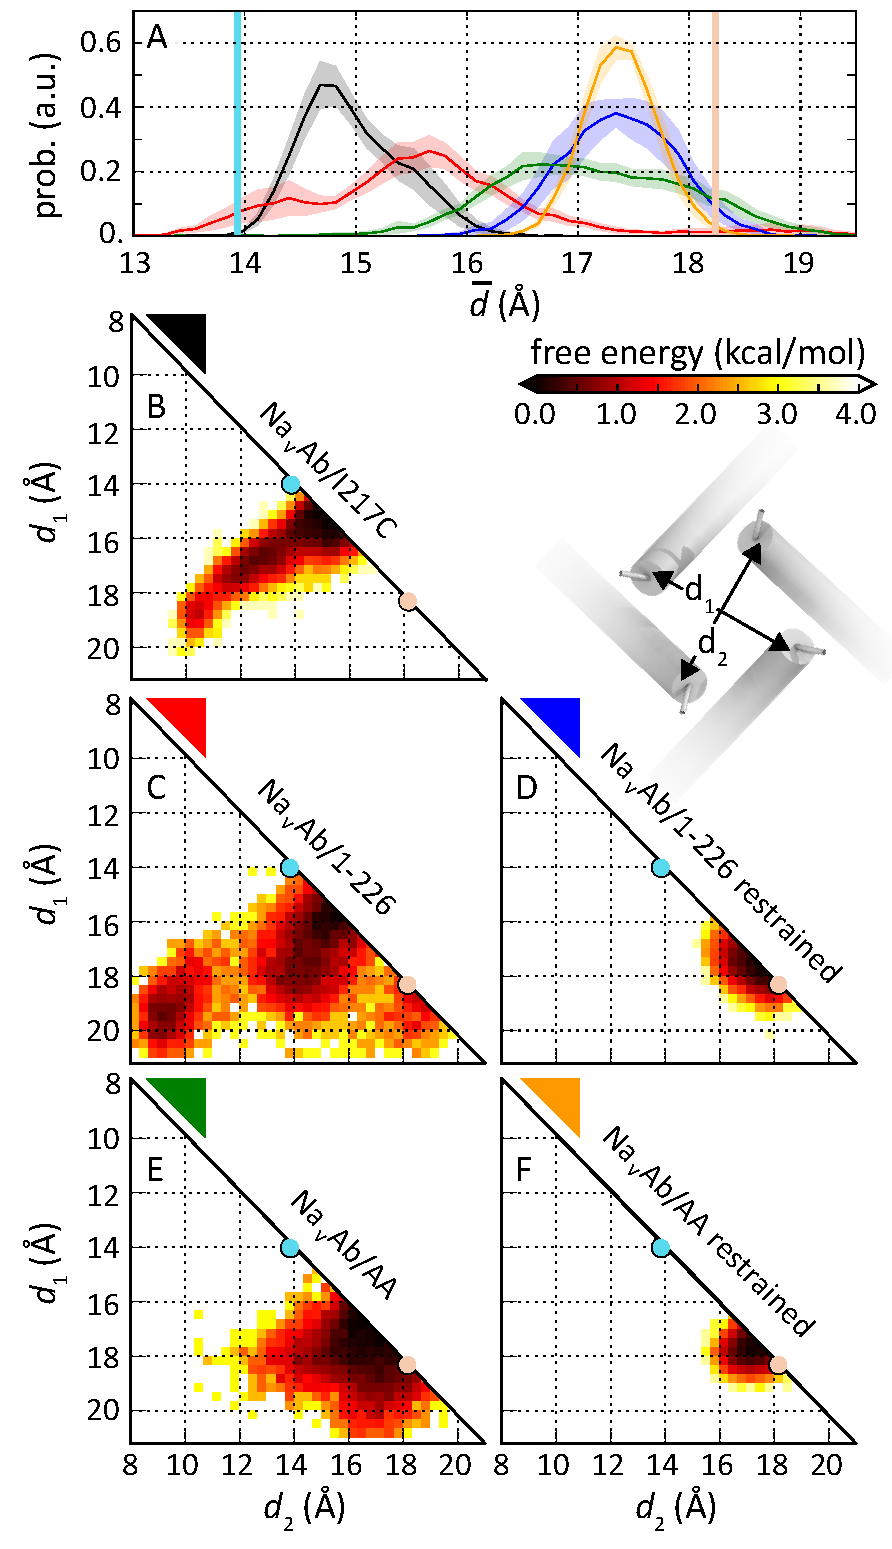
\includegraphics[width=0.5\textwidth]{navopen/NavOFig9}
\caption[Structural fluctuations of the activation gate]{\textbf{Structural fluctuations of the activation gate}. (\textbf{A}) Probability distribution of the mean diameters of the activation gate. NaVAb/I217C, black; NaVAb/1-226 restrained open, blue; NaVAb/1-226, unrestrained, red; NaVAb/AA restrained open, tan; NaVAb/AA unrestrained. a.u., arbitrary units; prob., probablility. (\textbf{B}) Free energy of the pairwise distances of residue 215-218 C$\alpha$ atom center of mass in diagonal subunits, d1 and d2, from molecular simulations with several channel models. (\textbf{B-F}) Free energy profiles are shown for: top row, NaVAb/I217C preopen state without TM restraints (black; \textbf{B}); middle row, NaVAb/1-226 without (red; \textbf{C}) and with (blue; \textbf{D}) TM restraints; and bottom row, NaVAb/V213A/C217A (NaVAb/AA) without (\textbf{E}) and with (\textbf{F}) TM restraints. The average pairwise distance of diagonal subunits in the open- and closed-state crystal structures are shown as pink and blue circles, respectively. Inset, a schematic representation of distances d1 and d2.}
\label{fig:navofig9}
\end{figure}

To examine the interplay of hydration, ion permeation, and structural fluctuations of the activation gate, we performed multiple MD simulations of NaVAb/I217C and NaVAb/1-226 in a hydrated lipid bilayer in the microsecond time range (Methods). Because the NaVAb/1-226 structure is a static snapshot of an apparently open conformation of the activation gate, we first examined results obtained by using harmonic restraints to keep the S6 helices close to the crystallographic structure of the open state. In these simulations, we observed a distribution of pore diameters at the centers of the S6 helices at the activation gate (Fig. \ref{fig:navofig9} A, blue), with a mean of $17.4 \pm 0.1$ \AA. In this restrained open state, there were relatively small fluctuations in the asymmetry of the S6 helices, as illustrated by the small deviations from the diagonal line in Fig. \ref{fig:navofig9} D. The mean hydration of the activation gate in this open-state structure was $15.1 \pm 0.8 $ water molecules (Fig. \ref{fig:navofig10} A, blue). Na$^+$ moved through this bottleneck with an average of $ 5.3 \pm 0.1$ water molecules in its inner hydration shell, compared with $5.8 \pm 0.1$ in free solution, indicating that passage through the open activation gate requires only the loss of $\sim$ 0.5 water molecule in the inner hydration shell of Na$^+$ (Fig. \ref{fig:navofig10} D). The estimated free energy barrier for Na$^+$ permeation was $\sim$2 kcal/mol (Fig. \ref{fig:navofig10} F), comparable with the free energy barrier for movement of Na$^+$ through the selectivity filter \cite{Chakrabarti:2013kd}. Together, these results are consistent with the conclusion that the NaVAb/1-226 structure captured by X-ray crystallography has an open activation gate, which presents no significant barrier to Na$^+$ permeation.

To study the effect of thermal fluctuations of the activation gate, we conducted similar simulations without restraints. In unrestrained simulations initiated in the NaVAb/1-226 or the NaVAb/I217C conformation, the activation gate spontaneously underwent moderate contraction and dilation, with changes in the average diagonal distances from the centers of the cylinders of the S6 $\alpha$ helices from $18.2 \rightarrow 15.7 \pm 0.2$\AA  and $13.9 \rightarrow 15.0 \pm 0.1$ \AA, respectively (Fig. \ref{fig:navofig9} A, black and red). Thermal fluctuations often led to significant deviations from the symmetric arrangement of the S6 helices, as shown by the deviations from the diagonal line in Fig. \ref{fig:navofig9} B (black and red). The activation gate bottleneck was completely dehydrated (dewetted) in the NaVAb/I217C preopen state (Fig. \ref{fig:navofig10} A-C, black), whereas it fluctuated between 0 and 25 water molecules, with an average of $7.3 \pm 0.4$, in unrestrained NaVAb/1-226 (Fig. \ref{fig:navofig10} A-C, blue).
To examine the effect of the hydrophobic side chains on the structure and properties of the activation gate, we replaced both C217 and V213 by alanine (NaVAb/AA) and repeated the simulations successively with and without restraints on helix position. In the restrained simulations, this double mutation resulted in a shift of helix geometry toward the open state relative to WT ($17.5 \pm 0.1$ vs. $15.7 \pm 0.2 $ \AA; Fig. \ref{fig:navofig9} A, D, and E) and greater hydration (Fig. \ref{fig:navofig10} A-C). Because of the smaller side chains, average pore hydration in NaVAb/AA was greater than in NaVAb/I217C in both unrestrained and restrained simulations ($20.5 \pm 0.6$ and $21.3 \pm 0.2$ water molecules, respectively). As such, Na$^+$ hydration in the activation gate only dropped to $5.5 \pm 0.1$ in the double mutant (Fig. \ref{fig:navofig10} D). However, this additional hydration had no effect on the free energy barrier for Na$^+$ movement, which was indistinguishable from that obtained from restrained simulations of the open NaVAb/I217C channel (Fig. \ref{fig:navofig10} F).

Together, the MD simulation results confirmed that the crystallographic structure of NaVAb/1-226 corresponds to an open state of the NaVAb pore, for which the activation gate induces a small desolvation penalty of $\approx$2 kcal/mol relative to the aqueous state. Structural relaxation led to a partial collapse and partial dehydration of the activation gate, which resulted in doubling the height of the Na$^+$ desolvation barrier to 4 kcal/mol, and to asymmetric fluctuations of the activation gate that were also observed in the closed state of the channel. These effects all but disappeared in the NaVAb/AA double mutant of the S6 helix, which remained close to the crystallographic structure of the open state, even in the absence of helix restraints. These results support a hydrophobic-collapse model for closure of the activation gate.

\begin{figure}[hp]
\centering
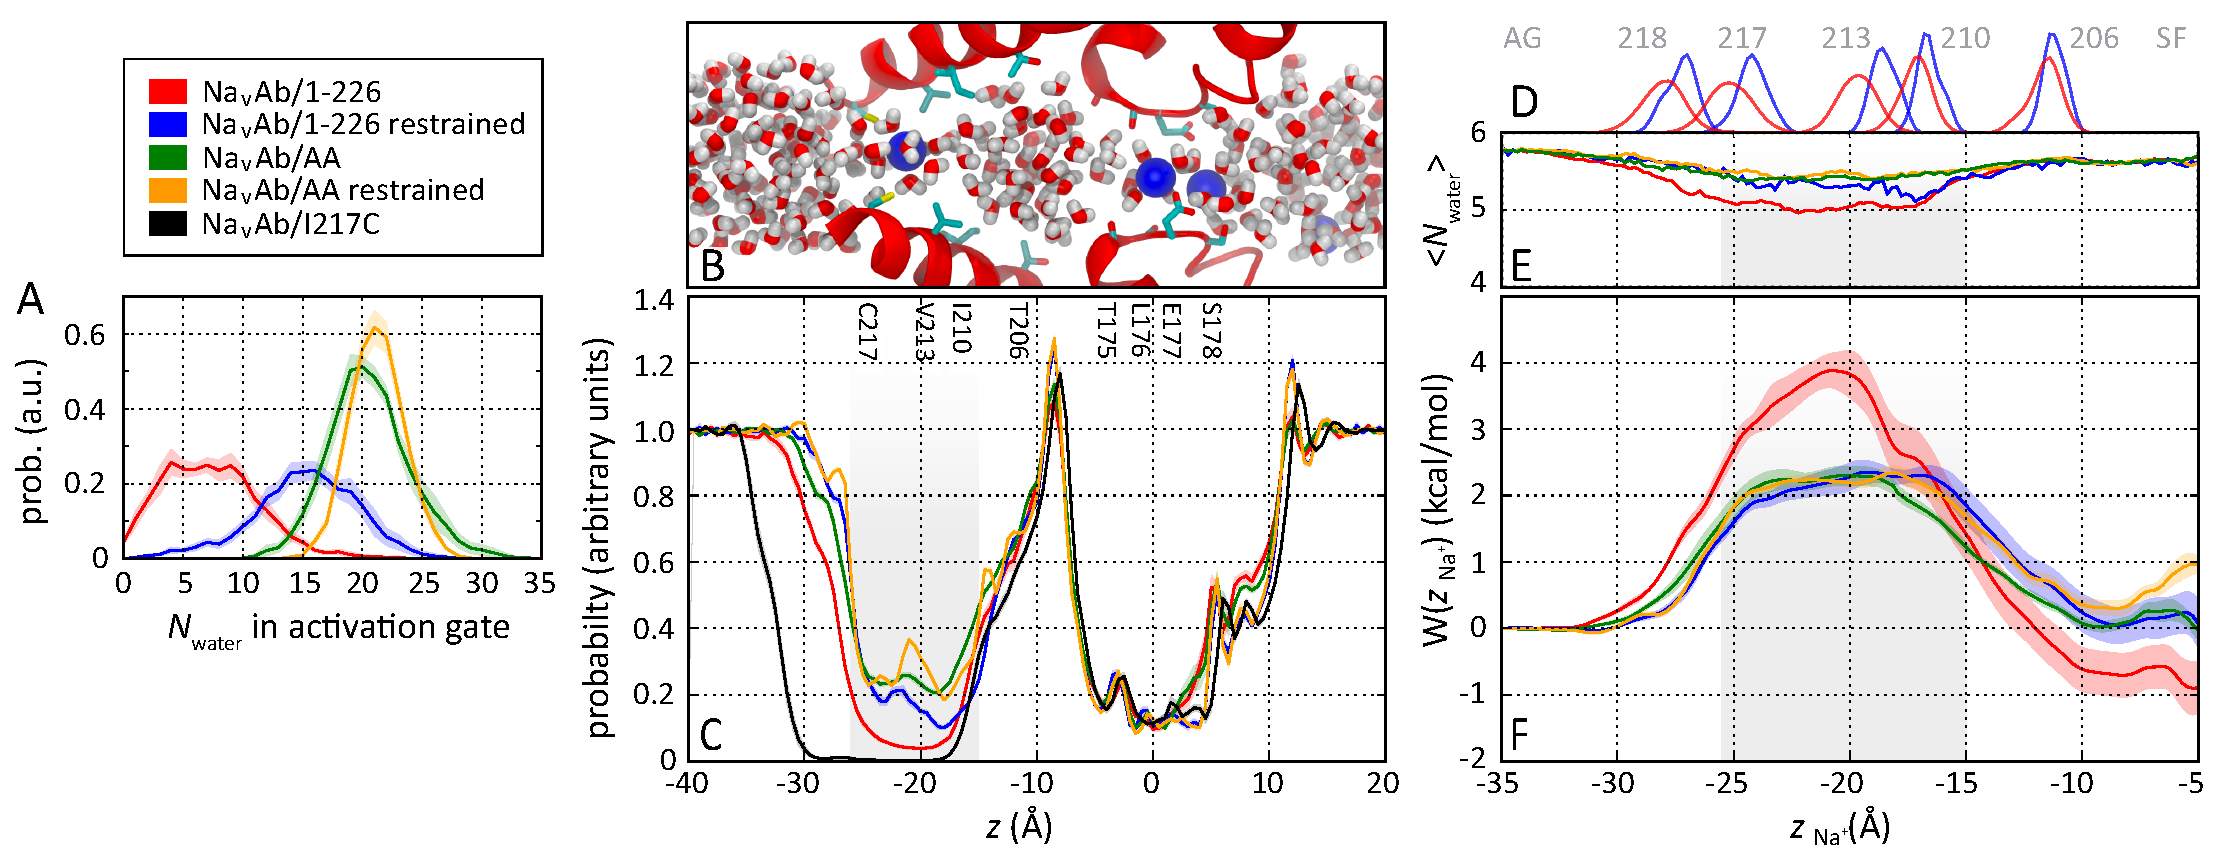
\includegraphics[width=0.9\textwidth]{navopen/NavOFig10}
\caption[Hydration and free energy of Na$^+$ conduction through the activation gate]{\textbf{Hydration and free energy of Na$^+$ conduction through the activation gate}. (\textbf{A}) Distribution of the number of water molecules, $N_{water}$, in the activation gate. Color coding is indicated in the key. (\textbf{B}) Snapshot of the unconstrained NaVAb/1-226 I217C channel with one Na$^+$ cation in the activation gate and two Na$^+$ cations in the selectivity filter shown as blue spheres. Two pore domain monomers are shown as red ribbons with selected side chains indicated below. Water molecules are shown as red and white licorice. (\textbf{C}) Distribution of water molecules along the pore axis. Scale and alignment are identical to \textbf{B}. The activation gate is highlighted in gray shading. (\textbf{D}) Axial distribution of C-alpha atoms of selected side chains lining the activation gate and the CC of the channel from restrained (blue) and unrestrained (red) simulations of NaVAb/1-226 I217C. AG, activation gate; SF, selectivity filter. (\textbf{E}) Average number of water molecules in the first hydration shell of Na$^+$ from bulk water (left) to the CC (right). (\textbf{F}) PMF profiles W($z_{Na^{+}}$) for movement of a Na$^+$ ion along the pore axis. Differences in the free energy of Na$^+$ in the CC (z > $\sim$15 \AA) are due to fluctuations in the number of cations present in the selectivity filter. In \textbf{C}, \textbf{E}, and \textbf{F}, the 11 \AA-wide barrier region is highlighted in gray shading. Data for NaVAb/I217C are only shown in \textbf{C} because the long, narrow dehydrated intracellular activation gate and the passage of Na$^+$ ions.}
\label{fig:navofig10}
\end{figure}

\section{Discussion} 

\subsection{S6 Mutations Reveal the Structure of NaVAb's Intracellular CTD}
Our FY structure revealed the conformation of the CTD of NaVAb in a closed state of the pore. It is a four-helix bundle similar to that observed in other BacNav channels and prokaryotic K$^+$ channels, as well as the pore-only construct of NaVAep1 and a NaK chimera \cite{Irie:2012dn,Arrigoni:2016fs}. In the highest-resolution structure of NaVAep1 (2.95 \AA), the portion of the CTD nearest to the pore contained a pi-helix that accommodated a centrally oriented tryptophan residue coordinating a chloride ion in the middle of the four-helix bundle. The NaVAb structure lacks this feature. Instead, there is a continuous alpha helix with two centrally oriented rings of polar residues (N225 and E228) in an equivalent position. This structure of the C terminus of NaVAb may contribute to its voltage dependence of activation, because removing the C terminus in NaVAb/1-226 favored channel activation and pore-opening.

\subsection{Closed States of the Pore}
The FY mutation rendered the pore of NaVAb/FY constitutively closed at the intracellular activation gate, even though three gating charges in the voltage sensors were in their outward, activated positions. Upon depolarization from the very negative membrane potential characteristic of the resting state of NaVAb (less than -180 mV) \cite{Payandeh:2012ib,Payandeh:2013ex}, the S4 segments in the voltage-sensing modules are thought to move outward in response to the change in electrical field to reach an activated state, but the FY mutation has trapped the pore in a tightly closed conformation characteristic of the deeper resting states of NaVAb. The mutation in NaVAb/FY may prevent the kink and rotation of the S6 segment that opens the pore, and thereby uncouple the conformational change of the voltage sensor from opening the activation gate because of the high energy needed to rewet and open the dehydrated, closed activation gate. It is also conceivable that the NaVAb/FY structure represents an artifactual state of the activation gate imparted by the introduction of bulky hydrophobic residues in S6, but we consider this possibility to be unlikely because the mutations made are characteristic of mammalian NaV channels, and the voltage sensor continues to function normally. Moreover, the structure of NaVAb/1-238 has a similar deeply closed activation gate with no mutation in the S6 segment \cite{Lenaeus:2017bf}. Mammalian sodium channels may have a larger CC that accommodates the movements of the FY residues without uncoupling from the normal voltage-sensing and gating cycle. Further support for the significance of the structure of NaVAb/FY comes from comparison with MD simulations of KV channels. In long simulations of Kv gating, large hyperpolarizations caused the pore to collapse and dehydrate, expelling water from the CC \cite{Jensen:2012ee}. The resulting KV channel structure resembles the NaVAb/FY structure in this respect, because the cavity of NaVAb/FY would contain far fewer water molecules than that of NaVAb/I217C or NaVAb/1-226.

NaVAb/FY has three characteristics expected of a closed state. First, the bundle crossing is tightly closed, with narrowing at I217 and M221, making the orifice small enough to occlude hydrated Na$^+$. Second, the S6 helix maintained its helical conformation throughout its entirety (Fig. 3C), a feature known to favor the closed state based on previous electrophysiological data in NaChBac and analysis of the open form of the pore-only NaVMs construct \cite{Zhao:2004vo,Bagneris:2013bu}. Third, the S6 bundle crossing and selectivity filter have not adopted the asymmetric conformation previously observed in the inactivated state structures of NaVAb and NaVRh (8, 9). We believe this structure represents a previously unrecognized view of a ``fully closed'' activation gate in a BacNav channel and provides a starting point for more refined models of pore opening in these channels and their eukaryotic homologs.

The NaVAb/FY structure further demonstrates the structural plasticity of the S4-S5 linker region, as previously suggested by comparison of the inactivated-state structure of NaVAb/WT compared with that of NaVAb/I217C \cite{Payandeh:2013ex}. The C-terminal region of the S4-S5 linker, in particular, has been found in multiple conformations in BacNav structures, suggesting a key role for residues 128-133 in gating of NaVAb. This region has also been found in different conformations in TPC structures \cite{Guo:2016jb,Kintzer:2016eu}. Comparison of mammalian sequences shows a general pattern of flexible amino acids with a conserved hydrophobic ``finger'' (either L or I) at the position corresponding to NaVAb M130. Our data suggest that this position tunes channel opening by functioning as both a hydrophobic barrier to excess opening of the channel's permeation pathway, as well as a pinch point that can bend the S6 below the level of the activation gate.

\subsection{Open State of the Pore}
Our C-terminal truncation of NaVAb favors the transition to the open state in situ. We believe that our structure of the NaVAb/1-226 indeed represents an open state of NaVAb for three reasons. First, the S6 helix has adopted the kinked conformation suggested in prior structure-function studies of NaChBac (26, 27, 37) \cite{Zhao:2004vo} and the pore-only open-state structure of NaVMs \cite{McCusker:2012di} (Fig. \ref{fig:navofig3} B and C). Second, crystallographic B factors are increased in this region of the protein relative to surrounding residues, suggesting an increase in flexibility and thermal motion. Third, the width across the bundle crossing, measured from the centers of the nearest atoms, has increased approximately twofold at the level of residue 217, to a distance that would accommodate the passage of hydrated Na$^+$ according to our MD simulations. Flexibility by way of kinking and bending motions are common features of membrane proteins and transporters, and represent relatively low-energy ways to impart structural change in a membrane environment \cite{Wilman:2014fk}. They are also seen in a number of related proteins including prokaryotic K$^+$ channels, where an analogous position serves as both a gating hinge and a modulator of inactivation \cite{Cuello:2010kf,Jiang:2002fx,Zhou:2001vo}.
In the structure of NaVAb/1-226, additional outward movement of the S6 segments away from the central axis would be prevented by the S4-S5 linkers from each subunit, which form a square corral to prevent further opening. The bulky side chain of M130 causes steric hindrance with that of I216 and prevents further movement, and the side chain of M130 has taken the position that would normally be taken by that of I216 if S6 were to remain an ideal alpha-helix. In this region, the conformation of NaVAb with intact voltage sensors differs from the open state structure of NaVMs with voltage sensors deleted because in NaVMs there is no S4-S5 linker helix. Lacking the constraint of the S4-S5 linker, the residue that is equivalent to I216 in NaVMs lies in a position that would clash with the S4-S5 linker, whereas I216 is rotated away from this position by way of the helix kink in NaVAb/1-226. Because of the constraints imposed by the S4-S5 linker, we believe that the structure of NaVAb/1-226 represents the most open conformation possible for the S6 activation gate in NaVAb.

\subsection{Gating of Cation Permeation by Hydrophobic Collapse}

The interplay of pore dilation, hydration, and free energy for ion permeation observed in our MD simulations is consistent with the notion of a hydrophobic activation gate, as previously proposed for other ion channels, including KV channels \cite{Jensen:2010fd,Aryal:2015ge,Zhu:2012ch,Neale:2015ee}. In a hydrophobic gate, changes in the size of a narrow hydrophobic segment of the lumen shift the equilibrium between hydrated (wetted) and dehydrated (dewetted) states, enabling or precluding the passage of ions. As such, sharp wetting/dewetting transitions that are coupled to changes in the relative arrangement of pore helices mediate opening and closing of the activation gate. Consistent with such a hydrophobic gating mechanism, in our MD simulations of the NaVAb/I217C and NaVAb/1-226 channels, the closed conformation is characterized by a persistent dewetted state, whereas in the open state, the water count in the activation gate undergoes fluctuations between wetted and dewetted states. Furthermore, not only does the NaVAb/AA mutation free up space in the hydrophobic bottleneck by reducing the length of side chains, but also the pore helix bundle is more dilated than in NaVAb/1-226, indicating coupling between hydrophobic collapse of the side chains in the activation gate and pore helix contraction. When the hydrophobic cavity is small because of larger hydrophobic side chains, the pocket is dewetted and collapses, whereas when the cavity is larger because of smaller hydrophobic side chains, the activation gate is hydrated and expands. Thus, pore dilation and hydration reinforce each other. In NaVAb/AA, the cavity is large enough to displace the equilibrium toward the wetted state, and the S6 helices relax to a more open arrangement. The fact that the additional hydration in NaVAb/AA does not change the small desolvation penalty for movement of Na$^+$ confirms that the crystallographic structure of NaVAb/1-226 corresponds to the fully open state of the activation gate.

\subsection{Implications for State-Dependent Drug Binding} 

Local anesthetic and antiarrhythmic drugs are thought to bind to a receptor site in the CC of the pore \cite{Hille:2001tw}. Frequent opening of the pore enhances drug binding and block. Our structure of NaVAb/1-226 reveals how these drugs gain access to their receptor site, because the diameter of the open activation gate (10 \AA) is large enough to allow passage of typical local anesthetic and antiarrhythmic drug molecules. Bound local anesthetic and antiarrhythmic drugs are expelled from their receptor site by strong hyperpolarization \cite{Hille:1977td,Courtney:1975uu}. Our structure of NaVAb/FY illustrates a possible mechanism for this canonical feature of drug block. In the state captured in this structure, the S6 segments lining the CC have changed conformation in the closed and open states we have characterized here, and the side chains of key amino acid residues have moved significantly. Therefore, voltage-dependent unblocking of NaV channels may result from hyperpolarization-dependent transition to a deep resting state similar to NaVAb/FY and the deep resting states observed in MD simulations of KV channels \cite{Jensen:2012ee}, which have an altered conformation of the drug binding site in the CC.

\subsection{Refining the Closed-Open-Inactivated Model for NavAb}

Models of pore domain movement have been incomplete because of the absence of a closed activation gate structure in a full-length channel and the absence of a voltage sensor in the pore-only models of the open state \cite{Bagneris:2014eh,Guo:2016jb,Kintzer:2016eu}. Models of activation gating in NaV channels were heavily influenced by the putative hinge glycine in prokaryotic K$^+$ channels \cite{Jiang:2002fx}, which plays a key role in the activation of NaChBac \cite{Zhao:2004vo,Shafrir:2008ic}. However, other BacNav orthologs do not have a glycine in the equivalent position and lack an obvious hinge residue in the S6 segment. The structure of NavAb/I217C suggested a key state-dependent interaction of the voltage sensor with the base of S5 and subsequent iris-like dilation of the activation gate caused by subtle bending and twisting motions distributed along the S6 segment \cite{Payandeh:2012ib}. A pore-only model of the open state suggested that activation gating occurs with a local bending motion in S6 \cite{Bagneris:2014eh}, similar to that suggested in the original glycine hinge models \cite{Zhao:2004vo,Jiang:2002fx,Zhao:2004vv}. Our data refine these models by identifying two previously unrecognized conformations of NaVAb's S6 helix, a straight form present when the pore is tightly closed and a kinked form that develops during pore opening, probably in concert with movement in the voltage sensor, the S4-S5 linker, and the S5 segment. In this revised model, gating begins with movement in the S4 segment, which is then coupled to movement in the S4-S5 linker, and propagated to S5 and S6 through internal protein interactions. These motions of the S5 and S6 segments have direct effects at the activation gate and indirect effects that allow the S6 segment to adopt the kinked conformation visualized in the NaVMs and NaVAb/1-226 structures. Our truncated NaVAb/1-226 construct has allowed visualization of the kinked form due to removal of its natural constraint, the CTD. The twisting/bending motion of the rigid helical form of S6 may be driven in part by exchange of hydrogen bonds of T206 from the nearby pore helix to the S6 helix itself.

\subsection{Comparison with Gating of Eukaryotic NaV Channels} 
Studies of cysteine accessibility suggested that the activation gate in NaV1.4 is located at the position of I217 in NaVAb \cite{Oelstrom:2016dl,Oelstrom:2014ky}. These data are in good agreement with our structures and suggest that the activation gate in BacNavs is similar to that in NaV1.4 domain IV, consisting of a hydrophobic barrier at the position of I217. M221 provides another hydrophobic barrier to permeation in NaVAb and some other BacNav structures. The analogous residue does not prevent access of cysteine probes to S6 residues in domain IV in the resting state of NaV1.4, but the residues present at equivalent locations in other domains of eukaryotic NaV channels may restrict passage through the activation gate.
Our data also inform modeling of activation gating in vertebrate NaV channels, particularly with regard to conformational changes in the S6 segment. The residue homologous to T206 is coupled to movements of the domain III voltage sensor, as assessed by voltage-clamp fluorometry studies of NaV1.5 \cite{ArcisioMiranda:2010gz,Muroi:2010do}. It has also been hypothesized as a gating hinge for opening movements of D1-D3 in NaV channels \cite{Zhao:2004vo}. Sequence alignment of human isoforms of NaV channels shows that this residue and its neighbor are highly flexible in D1-D3, with each one containing a glycine and a small polar amino acid, either serine or asparagine. Such combinations are likely to produce helical breaks or kinks similar to the one we have identified in NaVAb/1-226, and this process may explain the differential kinetics between opening of D1-D3 and D4, which has the less flexible amino acids SF in this location \cite{Chanda:2002gk}. Our results support the hypothesis that D1, D2, and D3 pore domains open more easily due to conformational flexibility in the S6 segment, whereas D4 opens more slowly due to the more rigid S6 conformation noted. This portion of the channel also plays a key, rate-limiting role in fast inactivation \cite{Capes:2013cc}.

\section{Methods} 

%\subsection{NavAb Crystallization and Data Collection} NavAb/FY and NavAb/1-226 were reconstituted into 1,2-dimyristoyl-sn-glycero-3-phosphatidylcholine (DMPC): CHAPSO bicelles (Anatrace) as described (7), and then mixed in a 1:2 ratio and set up in a hanging-drop format over well solutions containing 1.8 M ammonium sulfate and 100 mM sodium acetate (pH 4.8). Crystals appeared in 3-5 d and grew to full size within 1 wk (~50 by 100 $\mum$). They were cryoprotected by slow addition of well solution supplemented with increasing concentration of glucose. Final glucose concentration was 30\% after this procedure, and then crystals were harvested in nylon loops and plunged into liquid nitrogen for data collection. Data were collected at Advanced Light Source (beamlines BL821 and BL822), with diffraction quality and resolution substantially improved from previous reports. Most NavAb crystals diffracted to better than 4 $\AA$ - the data reported herein were collected from single crystals, collected at 0.9999-1.1000 $\AA$. As reported previously, crystals were highly radiation sensitive, and exposure times were minimized to limit decay during data collection.

%\subsection{Structure Determination and Refinement}
%X-ray diffraction data were integrated and scaled with DENZO/SCALEPACK (51), and then processed with PHENIX (52). The NaVAb/FY structure was solved with molecular replacement by using the voltage sensor and selectivity filter of NaVAb [Protein Data Bank (PDB) ID code 3RVY] as search model. The NaVAb/1-226 structure was solved with molecular replacement, by using the voltage sensor of NaVAb/I217C as a starting model. After initial phases, models of both proteins were manually rebuilt based on resulting electron-density maps. Tight non-crystallographic symmetry restraints were applied throughout the early stages of refinement of NaVAb/FY and clearly improved our electron-density maps. Electron density was easily interpretable throughout the CTD for all four chains of NaVAb/FY, although side chains could not be visualized near the C terminus. As noted in the text, electron density was weak for the C-terminal portion of S6 of NaVAb/1-226 and could not be modeled for any amino acids past D219. Simulated annealing omit maps were used to confirm the placement of the S6 at the activation gate, as well as the position of the S4-S5 linker. Lipids and waters were added to both models near the end of refinement, and then NCS restraints were relaxed in the final stages. Geometry, B factors, and electron-density fits were assessed with POLYGON (53).

%\subsection{Molecular Dynamics}

All-atom molecular models of the NaVAb I217C mutant (PDB code: 3RVY) \cite{Payandeh:2012ib} and the NavAb/1-226 I217C mutant were constructed by embedding them in a hydrated 1,2-dimyristoyl-sn-glycero-3-phosphatidylcholine (DMPC) bilayer, with 270 and 280 lipid molecules respectively. The NavAb I217C simulation system consisted of a periodic rectangular cell comprised of ~129,000 atoms with approximate dimensions of 10.9 $\times$ 10.9 $\times$ 10.2 $nm^{3}$. The NavAb/1-226 I217C simulation system consisted of a periodic hexagonal cell comprised of ~145,000 atoms with approximate dimensions of 12.1 $\times$ 10.5 $\times$ 10.8 $nm^{3}$. ~250 mM (122 Na$^+$ and 130 Cl-) and ~170mM NaCl (93 Na$^+$ and 109 Cl-) were present in the NaVAb I217C and NavAb/1-226 I217C models, respectively. Membrane embedding was performed using the alchembed protocol (2) using an equilibrated rectangular CHARMM36 DMPC bilayer patch obtained from the Jeffery Klauda laboratory website (https://terpconnect.umd.edu/ ~jbklauda/ research/download.html) and a hexagonal DMPC bilayer patch generated with the CHARMM-GUI membrane builder \cite{Wu:2014uc}. The model of the open state with V213A/I217A mutations was created by modifying the NavAb/1-226 I217C structure after membrane embedding using MODELLER \cite{Fiser:2003we} with the simulation cell otherwise unchanged. The protein, lipids, and ions were modeled with the CHARMM36 all-atom force field \cite{Best:2012uu,MacKerell:1998tp,Klauda:2010tn}, and water molecules were modelled with TIP3P \cite{Jorgensen:1983ty}. NBFIX adjustments were made for Na$^+$ - backbone carbonyl oxygen atom interactions \cite{Noskov:2008jp}, as well as NBFIX corrections for Na$^+$ - lipid head group interactions \cite{Venable:2013ix}. 
All unbiased simulations were performed with GROMACS (Version 4.6.5) \cite{Pronk:2013ef} at constant temperature (300 K) and pressure (1 atm). Restrained models of NaVAb/1-226 and NaVAb/AA, were prepared by imposing harmonic potentials with force constants of 1 kcal/mol/$\angstrom^{2}$ on all C$\alpha$ atoms of transmembrane helices S5 and S6, restraining them near the crystallographic state. Fifteen simulation repeats were generated for the NaVAb/I217C system (1000 ns each), and 10 simulation repeats were generated for each of the four open-state systems (600 ns each), with aggregate simulation time of 39 $\mu$s. All replicas of all systems began with 30 ns of protein-restrained equilibration not included in analysis.
For the four open-state systems, snapshots were extracted from five in- dependent simulation repeats at t = 100 ns and were subsequently used as initial conditions for umbrella sampling (US) simulations. We used biased sampling to study the movement of Na$^+$ along the channel axis from within the CC to bulk water on the intracellular side of the membrane. Production simulations were performed for $\sim$55 ns per umbrella with a harmonic restraining potential force constant of 2.39 kcal/mol/$\angstrom^{2}$s and a flat-bottom cylindrical position restraint on the target Na$^+$. All US simulations were performed with GROMACS (Version 5.0.6) \cite{Abraham:2015gj}. The axial position of the permeating Na$^+$ was used to generate five independent potential of mean force (PMF) profiles, for each of the open systems. We report the average PMF for Na$^+$ movement along the channel axis with error bars computed by using the SE of mean over all five PMFs. The aggregate simulation time of the US simulations was $\sim$39 $\mu$s (715 windows in total, multiplied by 55 ns)

\printbibliography[heading=subbibnumbered,title={References}]
\end{refsection}
 \begin{refsection}
\chapter{Structural basis for gating pore current in periodic paralysis}

The contents of this section were adapted from an article published in the \textit{Nature}.\par
\bigskip
Reference: Jiang, D., Gamal El-Din, T.M., Ing C., Lu, P., Pom\`es, R, Zheng, N., and Catterall, W. A. (2018) Structural basis for gating pore current in periodic paralysis. \textit{Nature}, 557 (7706), 590-594.\par
\bigskip
Contributions: D.J., T.M.G.E.-D., C.I., P.L., R.P., N.Z. and W.A.C. designed experiments. D.J., T.M.G.E.-D., C.I. and P.L. conducted experiments. D.J., T.M.G.E.-D., C.I., R.P., N.Z. and W.A.C. analyzed the results. T.M.G.E.-D., C.I. and W.A.C. wrote the paper with input from all co-authors.

\newpage

\section{Summary}

Potassium-sensitive hypokalaemic and normokalaemic periodic paralysis are inherited skeletal muscle diseases characterized by episodes of flaccid muscle weakness \cite{Venance:2006fc,PMID:28939973}. They are caused by single mutations in positively charged residues (`gating charges') in the S4 transmembrane segment of the voltage sensor of the voltage-gated sodium channel Na\textsubscript{V}1.4 or the calcium channel Ca\textsubscript{V}1.1 \cite{Venance:2006fc,PMID:28939973}. Mutations of the outermost gating charges (R1 and R2) cause hypokalaemic periodic paralysis \cite{Venance:2006fc,PMID:28939973} by creating a pathogenic gating pore in the voltage sensor through which cations leak in the resting state \cite{Sokolov:2007iu,Struyk:2007jp}. Mutations of the third gating charge (R3) cause normokalaemic periodic paralysis \cite{Vicart:2004jh} owing to cation leak in both activated and inactivated states \cite{Sokolov:2008dv}. 

Here we present high-resolution structures of the model bacterial sodium channel Na\textsubscript{V}Ab with the analogous gating-charge mutations \cite{Payandeh:2012ib,Catterall:2015dha}, which have similar functional effects as in the human channels. The R2G and R3G mutations have no effect on the backbone structures of the voltage sensor, but they create an aqueous cavity near the hydrophobic constriction site that controls gating charge movement through the voltage sensor. The R3G mutation extends the extracellular aqueous cleft through the entire length of the activated voltage sensor, creating an aqueous path through the membrane. Conversely, molecular modelling shows that the R2G mutation creates a continuous aqueous path through the membrane only in the resting state. Crystal structures of Na\textsubscript{V}Ab(R2G) in complex with guanidinium define a potential drug target site. Molecular dynamics simulations illustrate the mechanism of Na$^+$ permeation through the mutant gating pore in concert with conformational fluctuations of the gating charge R4. Our results reveal pathogenic mechanisms of periodic paralysis at the atomic level and suggest designs of drugs that may prevent ionic leak and provide symptomatic relief from hypokalaemic and normokalaemic periodic paralysis.
	
\section{Introduction}

Na\textsubscript{V}1.4 channels generate action potentials that initiate muscle contraction \cite{Catterall:2005iw}. They are complexes of a pore-forming $\alpha$-subunit and auxiliary $\beta$1 subunits \cite{Catterall:2005iw,Shen:2017dfa,Yan:2017kda}. The $\alpha$-subunit contains four homologous domains (I-IV), each with six transmembrane segments (S1-S6). Segments S1-S4 form the voltage sensor, and every third residue in S4 is positively charged. Upon depolarization, S4 moves outward through a narrow gating pore formed by S1-S3, catalysed by interactions with negative or polar residues in S2 and S3 \cite{Catterall:2010kra}. The voltage sensor has an hourglass shape, with a narrow hydrophobic constriction site (HCS) that separates extracellular and intracellular compartments \cite{Payandeh:2012ib,Shen:2017dfa}. Water-filled crevices on either side of the HCS focus the membrane electric field, assuring efficient coupling of voltage to conformational changes that open the central pore \cite{Catterall:2010kra,Starace:2004ea}. Mutations in the arginine gating charges that occupy the HCS cause state-dependent cation leak through the voltage sensor, which we term `gating pore current' \cite{GamalElDin:2014gu,Sokolov:2010ii}.

Missense mutations of arginine gating charges in S4 of Na\textsubscript{V}1.4 cause hypokalaemic periodic paralysis and normokalaemic periodic paralysis \cite{PMID:28939973,JurkatRott:2012kv,Moreau:2014jy,Venance:2006fc}. Mutations of R1 in domains I or III to H or Q, or mutation of R2 in domains I, II and III to W, G, Q or S cause hypokalaemic periodic paralysis \cite{PMID:28939973,JurkatRott:2012kv,Moreau:2014jy,Venance:2006fc}. Mutations of R3 in domain II to G, Q or W, or of R3 in domain III to H or C cause normokalaemic periodic paralysis \cite{JurkatRott:2012kv,Moreau:2014jy,Struyk:2007jp}. All these mutations result in non-selective gating pore current through the voltage sensor \cite{JurkatRott:2012kv,Moreau:2014jy,Sokolov:2007iu,Struyk:2007jp,Wu:2012fj,Wu:2011il}. Increased inward leak leads to Na$^+$ overload, sustained depolarization and action potential failure, which paralyze skeletal muscles \cite{JurkatRott:2012kv,Moreau:2014jy,Sokolov:2007iu,Wu:2012fj,Wu:2011il}. These pathophysiological effects suggest that mutations that cause hypokalaemic periodic paralysis result in an open aqueous pathway for ion movement in the resting state of the voltage sensor, but not in the activated state, and mutations that cause normokalaemic periodic paralysis result in an open aqueous pathway in the activated state, but not in the resting state. Molecular models and mutagenesis studies support this hypothesis \cite{GosselinBadaroudine:2012eh,Monteleone:2017gj,Moreau:2015je}. To provide direct structural evidence for this pathophysiological mechanism, we introduced mutations known to cause periodic paralysis into Na\textsubscript{V}Ab, a voltage-gated Na$^+$ channel from Arcobacter butzleri, the structure of which has been solved at high resolution \cite{Payandeh:2012ib}. We characterized the resulting gating pore currents, solved the structures of mutant gating pores without and with a bound permeant ion, and investigated molecular dynamics \cite{Chakrabarti:2013kd} of ion movement through the gating pores.

\section{Results}

Pathogenic hypokalaemic periodic paralysis gating pore currents were reconstituted in Na\textsubscript{V}Ab by mutating R2 to S (R2S, analogous to Na\textsubscript{V}1.4(R672S)) \cite{Jiang:2018ga}. Electrophysiological measurements confirm a nonlinear leak current component in the resting state of the channel. Mutations of the gating charge R3 that cause normokalaemic periodic paralysis (Nav\textsubscript{V}1.4(R675G/Q/W)) induce outward gating pore current in activated but not in resting states. Na\textsubscript{V}Ab(R3G) conducted outward gating pore current in both activated and inactivated states \cite{Jiang:2018ga}. These physiological studies demonstrate that Na\textsubscript{V}Ab provides an accurate model of Na\textsubscript{V}1.4, because gating pore current is observed only in the resting state for Na\textsubscript{V}Ab(R2S) and only in the activated and inactivated states for Na\textsubscript{V}Ab(R3G).

%To reconstitute pathogenic hypokalaemic periodic paralysis gating pore currents in Na\textsubscript{V}Ab, we mutated R2 to S (R2S, analogous to Nav\textsubscript{V}1.4(R672S)) and expressed the mutant in Trichopulsiani insect cells. Transfected cells were voltage-clamped to ?200 mV and depolarized in 10-mV steps to record Na$^+$ currents. Half-maximal activation of central pore currents was observed at Va = ?105 � 0.6 mV (Fig. 1a). To measure gating pore currents, cells were held at ?100 mV, at which Na\textsubscript{V}Ab is in the slow-inactivated state and exhibits no central pore current. Gating pore current was examined by applying pulses from + 100 to ?200 mV in ?10 mV steps. A nonlinear leak current component was observed in the resting state, beginning at ?110 mV and increasing to ?200 mV (Fig. 1b, c).

%Mutations of the gating charge R3 that cause normokalaemic periodic paralysis (Nav\textsubscript{V}1.4(R675G/Q/W)) induce outward gating pore current in activated but not in resting states6. In Na\textsubscript{V}Ab(R3G), central pore current was activated between ?50 mV and 0 mV (Fig. 1d; Va = ?24.8 � 1.1 mV). Steady-state inactivation was observed from ?90 mV to ?10 mV with half maximal inactivation at Vh = ?47.7 � 0.4 mV (Fig. 1d). Na\textsubscript{V}Ab(R3G) conducted outward gating pore current in both activated and inactivated states at potentials more positive than ?60 mV (Fig. 1e, f ). These physiological studies demonstrate that Na\textsubscript{V}Ab provides an accurate model of Nav\textsubscript{V}1.4, because gating pore current is observed only in the resting state for Na\textsubscript{V}Ab(R2S) and only in the activated and inactivated states for Na\textsubscript{V}Ab(R3G).

The pathogenic effects of gating pore mutations depend on inward leak of Na$^+$. The R2S mutant gating pore was not significantly selective among Cs$^+$, K$^+$ or Na$^+$ \cite{Jiang:2018ga}. As is the case for Nav\textsubscript{V}1.424, the gating pore of Na\textsubscript{V}Ab(R2S) was exceptionally permeant to guanidinium (about 28-fold greater than Na$^+$), but it was less permeant to methyl-guanidinium and ethylguanidinium \cite{Jiang:2018ga}. The outward gating pore currents conducted by Na\textsubscript{V}Ab(R3G) were higher for Cs$^+$ than for K$^+$ or Na$^+$, which were similar to each other. However, Na\textsubscript{V}Ab(R3G) was less permeant to guanidinium than to Na$^+$, and it was more than 16-fold less permeant to guanidinium than Na\textsubscript{V}Ab(R2S) \cite{Jiang:2018ga}. The weak selectivity of R2S and R3G mutants for different inorganic cations and the high guanidinium permeability through the R2S mutant are characteristic of the corresponding mutations in Na\textsubscript{V}1.4 2, further supporting the validity of Na\textsubscript{V}Ab as a model for structural studies of gating pore mutations.

To elucidate the structure of a pathogenic gating pore in its conductive conformation in an activated voltage sensor, we solved the structure of a Na\textsubscript{V}Ab analogue of a normokalaemic periodic paralysis-causing mutation, Na\textsubscript{V}Ab(R3G), at 2.7 \AA resolution (Fig. \ref{fig:navVSDfig2}). Voltage-gated sodium channels have a central pore module surrounded by four symmetrically located voltage sensors (Fig. \ref{fig:navVSDfig2} A). The voltage sensors of Na\textsubscript{V}Ab and Na\textsubscript{V}1.4 are very similar in amino acid sequence and structure. The voltage sensors of wild-type (WT) Na\textsubscript{V}Ab and Na\textsubscript{V}Ab(R3G) crystallize in the same conformation, with a C$\alpha$ root mean square deviation (r.m.s.d.) of 0.39 \AA (Fig. \ref{fig:navVSDfig2} B). These results indicate that the R3G mutation does not perturb the overall structure of the voltage sensor and, therefore, that its pathogenic effects are caused by the loss of the R3 side chain. These channels crystallize with an activated voltage sensor \cite{Payandeh:2012ib} (Fig. \ref{fig:navVSDfig2} C), as would be expected at 0 mV. In Na\textsubscript{V}Ab(WT), R1, R2 and R3 are located extracellularly relative to the HCS, and their side chains point outward, toward the extracellular milieu (Fig. \ref{fig:navVSDfig2} C). By contrast, R4 is located intracellularly relative to the HCS and its side chain points inward towards the cytosol (Fig. \ref{fig:navVSDfig2} C). When viewed from the extracellular side, there is no water-accessible path into the cell through the wild-type voltage sensor (Fig. \ref{fig:navVSDfig2} D); however, we observed a deep solvent-accessible cleft extending down to the R4 side chain in Na\textsubscript{V}Ab(R3G) (Fig. \ref{fig:navVSDfig2} G).

\begin{figure}[!ptb]
\centering
\includegraphics[width=0.7\textwidth]{navvsd/NavVSDFig2}
\caption[Structures of the voltage sensor of Na\textsubscript{V}Ab(WT) and Na\textsubscript{V}Ab(R3G)]{\textbf{Structures of the voltage sensor of Na\textsubscript{V}Ab(WT) and Na\textsubscript{V}Ab(R3G)}. (\textbf{A}) Structure of Na\textsubscript{V}Ab(R3G) in top view. (\textbf{B}) Comparison of the conformations of Na\textsubscript{V}Ab(WT) (grey) and Na\textsubscript{V}Ab(R3G) (rainbow) voltage sensor in side view. (\textbf{C-E}) Structures of Na\textsubscript{V}Ab(WT) voltage sensor. (\textbf{C}) Side view highlighting gating charges in sticks. (\textbf{D}) Top view in space-filling format. (\textbf{E}) MOLE2 analysis of water-accessible space
in magenta. (\textbf{F-H}) Structures of Na\textsubscript{V}Ab(R3G) voltage sensor. (\textbf{F}) Side view highlighting gating charges. (\textbf{G}) Top view in space-filling format. (\textbf{H}) MOLE2 analysis of water-filled space in magenta. Green spheres in \textbf{F} and \textbf{H} indicate the positions of the missing side chain of R3. In \textbf{D} and \textbf{G}, the dotted red line circles the position where the gating pore would be in the activated state and the solid red line circles the open gating pore, respectively.}
\label{fig:navVSDfig2}
\end{figure}

Analysis of the structure of chain B of Na\textsubscript{V}Ab(WT) using the MOLE2 algorithm revealed an incomplete water-accessible path extending part of the way through the voltage sensor from both extracellular and intracellular sides, which is interrupted at the HCS by R3 (Fig. \ref{fig:navVSDfig2} E). Strikingly, in Na\textsubscript{V}Ab(R3G), the water-accessible path continues all the way through the voltage sensor, and has a diameter of 2 \AA at its narrowest point, similar to the size of Na$^+$ (Fig. \ref{fig:navVSDfig2} H). By contrast, in chain A, R4 was captured in a rotamer conformation in which the arginine side chain partially blocks the inner end of the gating pore in Na\textsubscript{V}Ab(R3G). Previously reported structures of Na\textsubscript{V}Ab in the slow-inactivated state show that R4 adopts four slightly different rotamer conformations, with the most open having a diameter of 3 \AA \cite{Payandeh:2012ex}. These results elucidate the molecular mechanism by which mutations in S4 cause pathogenic gating pore currents and suggest that ion permeation through the gating pore is controlled dynamically by the state of the voltage sensor and by rotamer conformations of R4.

In contrast to voltage-gated sodium-channel mutations that cause normokalaemic periodic paralysis, those that cause hypokalaemic periodic paralysis result in a channel that conducts gating pore current in the resting state but is closed in the activated state. Therefore, we hypothesized that Na\textsubscript{V}Ab(R2G) would not have a continuous water-accessible path through its gating pore in the activated state. Analysis of the 2.9 \AA structure of Na\textsubscript{V}Ab(R2G) revealed a gap with additional solvent-accessible area in the extracellular aqueous cleft in comparison to the wild-type channel, but no change in the backbone conformation (Fig. \ref{fig:navVSDfig3} A). Although the increased opening of the aqueous cleft in the voltage sensor is evident in space-filling models (Fig. \ref{fig:navVSDfig3} B), the R3 and R4 side chains seal the voltage sensor in this activated state, interrupting the transmembrane path and preventing ion conductance. The solvent-accessible area penetrates about 21 \AA into the membrane from the extracellular side (Fig. \ref{fig:navVSDfig3} C), more than 7 \AA deeper than in Na\textsubscript{V}Ab(WT) (Fig. \ref{fig:navVSDfig2} E), but it does not reach the cytosolic side. This structure illustrates why Na\textsubscript{V}Ab(R2G) does not conduct gating pore current in the activated state.

\begin{figure}[!ptb]
\centering
\includegraphics[width=0.7\textwidth]{navvsd/NavVSDFig3}
\caption[Structure of voltage sensor and guanidinium binding site of Na\textsubscript{V}Ab(R2G)]{\textbf{Structure of voltage sensor and guanidinium binding site of Na\textsubscript{V}Ab(R2G)}. (\textbf{A-C}) Structures of the activated voltage sensor of Na\textsubscript{V}Ab(R2G). (\textbf{A}) Side view with gating charges highlighted in sticks. (\textbf{B}) Top view in space-filling format. The dashed red line indicates the position of the closed gating pore. (\textbf{C}) MOLE2 analysis of water-filled space in magenta. (\textbf{D-F}) Rosetta structural models of resting state 2 of the voltage sensor were reoptimized with the amino-acid sequence of Na\textsubscript{V}Ab for Na\textsubscript{V}Ab(WT). (\textbf{D}) Na\textsubscript{V}Ab(R2G) (\textbf{E}) and Na\textsubscript{V}Ab(R3G). (\textbf{F}) The perspective is rotated approximately 180 degrees around the vertical axis to better illustrate the arginine gating charges in resting state 2. Green spheres represent missing arginine side chains of R2 and R3, respectively. Magenta blobs represent solvent- accessible volume modelled with MOLE2. (\textbf{G}) Top view of Na\textsubscript{V}Ab(R2G) with one guanidinium bound to each voltage sensor. (\textbf{H}) 2mFo-DFc electron density map (blue mesh) of residues around the guanidinium binding site at 1$\sigma$. (\textbf{I}) Interaction network between guanidinium and amino acids in the voltage sensor of Na\textsubscript{V}Ab(R2G). Grey dashed lines show interatomic distances shorter than 4 \AA.}
\label{fig:navVSDfig3}
\end{figure}

There are no crystal structures of the voltage sensor of a voltage-gated sodium channel in the resting state, because the resting state is only accessible at negative membrane potentials. However, we developed models of three resting states using disulfide locking of substituted cysteine residues and structure prediction with the Rosetta algorithm \cite{YarovYarovoy:2012et}; these are now considered consensus models of the actual resting states \cite{Catterall:2017if,Vargas:2012eka}. To model an open gating pore with the voltage sensor in the resting state, we introduced the R2G and R3G mutations into these resting-state models and analysed the resulting structures with the MOLE2 algorithm (Fig. \ref{fig:navVSDfig3} D-F). There is no continuous path through the voltage sensor in the wild-type resting-state structure (Fig. \ref{fig:navVSDfig3} D), whereas the resting state of the Na\textsubscript{V}Ab(R2G) voltage sensor contains a continuous water-accessible path through the membrane (Fig. \ref{fig:navVSDfig3} E). Loss of the R2 side chain leaves a gap at the HCS that is large enough for Na$^+$ to pass through (Fig. \ref{fig:navVSDfig3} E). By contrast, the transmembrane pathway is incomplete in Na\textsubscript{V}Ab(R3G) because the R2 side chain occupies the HCS and blocks the gating pore (Fig. \ref{fig:navVSDfig3} F). These structural models illustrate how R2 charge mutations that cause hypokalaemic periodic paralysis result in gating pore current in the resting state.

The Na\textsubscript{V}Ab(R2S) mutant channel is much more permeant than Na\textsubscript{V}Ab(R3G) to guanidinium ions \cite{Jiang:2018ga,Sokolov:2010ii}. Guanidinium ions are chemically similar to the distal moiety of the arginine side chain, and guanidine compounds with hydrophobic substituents can block mutant gating pores \cite{Sokolov:2010ii}. We probed our gating pore structures for guanidinium-binding sites by soaking crystals of Na\textsubscript{V}Ab(R2G) and Na\textsubscript{V}Ab(R3G) with guanidinium and methylguanidinium to determine whether they would bind in place of the missing side chain of R2 or R3. The crystal structures did not show guanidinium binding to Na\textsubscript{V}Ab(R3G). However, crystals of Na\textsubscript{V}Ab(R2G) soaked with guanidinium or methyl-guanidinium diffracted to 2.7 \AA and 2.5 \AA resolution, respectively, and unambiguous electron density was observed in place of each R2 side chain (Fig. \ref{fig:navVSDfig3} G-I). Bound guanidinium is clearly seen in 2Fo-Fc maps (Fig. \ref{fig:navVSDfig3} H). E32 and M29 from S1, N49 from S2, R1 and R3 from S4, and Q150 from an adjacent subunit form the binding site for guanidinium (Fig. \ref{fig:navVSDfig3} I). M29 and R3 each bind guanidinium through hydrogen bonds (Fig. \ref{fig:navVSDfig3} H,I). The carbonyl group of E32 and the carbonyl oxygen of R1 further lock guanidinium in place (Fig. \ref{fig:navVSDfig3} H,I). The binding site is flanked by hydrogen bonds from N49 and Q150 that stabilize guanidinium from opposite sides (Fig. \ref{fig:navVSDfig3} H,I). The binding site for methylguanidinium is almost identical. These structures capture guanidinium bound at a specific site in the closed R2G gating pore. The amino acid residues responsible for guanidinium binding are highly conserved in Na\textsubscript{V}Ab, Na\textsubscript{V}1.4 and Ca\textsubscript{V}1.1. Substituted guanidinium ions can block gating pore current without major effects on Na\textsubscript{V}1.4 function \cite{Sokolov:2010ii}, suggesting that guanidinium-containing compounds specific for this binding site could provide a basis for structure-based drug design and be used therapeutically to relieve the symptoms of hypokalaemic periodic paralysis.

To examine relationships among structural fluctuations of the gating pore, ionic hydration and Na$^+$ leakage, we performed molecular dynamics simulations of wild-type and R3G mutant voltage sensors in a hydrated lipid bilayer (Fig. \ref{fig:navVSDfig4}). Multiple unbiased simulation repeats, with a total duration of 30 $\mu$s, show that the overall structures are conserved. Analysis of axial distributions of water molecules revealed a narrow region (-5 \AA < z < 5 \AA) that is more hydrated in the R3G mutant than in the wild-type voltage sensor, owing to the larger size of the lumen in the mutant (Fig. \ref{fig:navVSDfig4} A-C, yellow; P < 0.002). The average count of water molecules within the HCS was $3.9 \pm 0.8$ and $5.3 \pm 0.4$ for the wild type and R3G mutant, respectively (Fig. \ref{fig:navVSDfig4} E). We performed umbrella sampling simulations to compute the free energy of Na$^+$ permeation along the principal axis of the voltage sensor. When Na$^+$ was within the HCS, the number of water molecules in the HCS increased to $8.4 \pm 0.3$ in the wild type and $9.0 \pm 0.3$ in the R3G mutant, respectively. The free-energy profile for Na$^+$ translocation forms a broad barrier spanning the HCS, centred at C$\alpha$ of R3. The R3G mutation significantly decreases the height of this barrier from $18 \pm 0.8$ to $11 \pm 1.4$ kcal mol$^{-1}$ (Fig. \ref{fig:navVSDfig4} E). These values are consistent with the undetectable gating-pore conductance in the wild type and an upper limit of around 0.1 pS in the R3G mutant \cite{Cooper:1988gh}. Analysis of ionic coordination shows that, at the extracellular edge of the barrier, the first solvation shell of Na$^+$ is almost exclusively composed of water, consistent with the hydrophobic nature of the bottleneck in the voltage sensor (Fig. \ref{fig:navVSDfig4} F). The total coordination number of $5.81 \pm 0.02$ in bulk water drops to $4.88 \pm 0.04$ at the peak of the free-energy barrier, suggesting a large desolvation penalty for Na$^+$ that is partly alleviated by the cavity created in the absence of the R3 side chain. Charge-charge repulsion is also likely to contribute substantially to the higher energy barrier to Na$^+$ permeation in the wild type, impeding the gating pore leakage observed in the R3G mutant.

\begin{figure}[!ptb]
\centering
\includegraphics[width=0.5\textwidth]{navvsd/NavVSDFig4}
\caption[R3G mutation lowers the free-energy barrier for Na$^+$ conductance]{\textbf{R3G mutation lowers the free-energy barrier for Na$^+$ conductance}. (\textbf{A}) Probability (prob.) distribution of water along the domain axis for Na\textsubscript{V}Ab(WT) (black) and Na\textsubscript{V}Ab(R3G) (red). (\textbf{B-C}) Representation of voltage sensor from Na\textsubscript{V}Ab(WT) and Na\textsubscript{V}Ab(R3G) simulations where Na$^+$ (blue sphere) is restrained at z = -5 \AA. The S2 segment (residues 45-65) is omitted for clarity. Arrows indicate the positions of R108. (\textbf{D}) Axial distribution of gating charge C$\alpha$ for Na\textsubscript{V}Ab(WT) and Na\textsubscript{V}Ab(R3G). The axial position in the crystallographic structure is shown as a vertical line. (\textbf{E}) Inset, probability distribution of water in the HCS (-5 \AA to 5 \AA) across all simulations of Na\textsubscript{V}Ab(WT) (black) and Na\textsubscript{V}Ab(R3G) (red). The total probability is separated into frames where Na$^+$ occupies the hydrophobic constriction (solid) or is outside this region (cross-hatched). $N_{wat}$, number of water molecules. Main panel, Potential of mean force for Na$^+$ conduction within the Na\textsubscript{V}Ab(WT) (black) and Na\textsubscript{V}Ab(R3G) (red) pore computed using umbrella sampling. The HCS is highlighted in yellow. (\textbf{F}) Average coordination of Na$^+$ as a function of ionic position along the principal axis of the voltage sensor, for Na\textsubscript{V}Ab(WT) (solid lines) and Na\textsubscript{V}Ab(R3G) (dashed lines). The first coordination shell of Na$^+$ is partitioned for coordination to protein (green), water (blue), lipid head groups (orange) and counterions (purple). (\textbf{G-I}) Representative snapshots from simulations of Na\textsubscript{V}Ab(R3G) depicting conformational isomerization of R4. *P < 0.002, n = 60. Arrow in g indicates the point of minimum coordination of Na$^+$ by water.}
\label{fig:navVSDfig4}
\end{figure}

The location of R4 coincides with a secondary shoulder in the free-energy profiles (Fig. \ref{fig:navVSDfig4} D, R108), indicating that movement of Na$^+$ past R4 is not rate-limiting for permeation, even though transit of Na past R4 causes the largest displacement of water by protein ligands (Fig. \ref{fig:navVSDfig4} E). Spontaneous disruption of the R4-E59 salt bridge in $3 \pm 1$\% of simulation frames for the wild type and R3G mutant opens the inner end of the gating pore with sufficient frequency to support gating pore current (Fig. \ref{fig:navVSDfig4} G-I). Na$^+$ often makes direct contacts with the anionic side chains of D80 and E59 (Fig. \ref{fig:navVSDfig4} F,G), and its movement is coupled to dynamic rearrangements of the R4 salt-bridge network.

\section{Discussion}
Overall, our results provide an unprecedented high-resolution view of functional effects of ion channel mutations that cause periodic paralysis and define the structural basis for pathogenesis of this ion channelopathy. R2G and R3G mutations do not perturb the backbone structure of the voltage sensor, suggesting that the aberrant gating pore currents are not caused by conformational changes in transmembrane alpha helices. Instead, the absence of the positively charged R2 and R3 side chains opens an aqueous gating pore that allows diffusion of Na$^+$ into the cell, depending on the functional state of the voltage sensor. Our structural studies show how this pathogenic gating pore current is gated in resting and activated states by transmembrane movements of the S4 segment. Although our studies of R2G and R3G mutants suggest a straightforward explanation for the pathogenic gating pore current, mutations that cause hypokalaemic periodic paralysis and normokalaemic periodic paralysis that substitute large side chains such as tryptophan also cause gating pore currents \cite{JurkatRott:2012kv,Moreau:2014jy,Struyk:2007jp}, perhaps by perturbing the local structure of the voltage sensor and thereby opening a pore across the membrane.

Our structures reveal the binding pose of a highly permeant ion, guanidinium, in the closed gating pore of the activated voltage sensor of Na\textsubscript{V}Ab(R2G). Substituted guanidinium derivatives can block gating pore current without impairing voltage sensor function in Na\textsubscript{V}1.4 \cite{Sokolov:2010ii}. Therefore, our high-resolution structural models may provide molecular templates for design and development of drugs that would mimic guanidinium, block gating pore current and provide symptomatic relief of periodic paralysis.

\section{Methods} 

Methodological details concerning electrophysiology, protein purification, crystallization, structural data collection, structure determination are reported in Jiang\textit{et al.} \cite{Jiang:2018ga}.

Molecular models of the Na\textsubscript{V}Ab(WT) and Na\textsubscript{V}Ab(R3G) channels were constructed using the Na\textsubscript{V}Ab(I217C) structure (PDB code: 3RVY) \cite{Payandeh:2012ib}. The latter model was generated by substituting R105 with G in all four voltage sensing domains. Both systems were embedded in a hydrated 1,2-dimyristoyl-sn-glycero-3-phosphatidylcholine (DMPC) bilayer with ~250 mM NaCl for a total of ~129,000 atoms. Embedding was performed using the alchembed protocol \cite{Jefferys:2015jt} using an equilibrated rectangular CHARMM36 DMPC bilayer patch obtained from the Klauda laboratory website (https://terpconnect.umd.edu/~ jbklauda/). The protein, lipids and ions were modelled with the CHARMM36 all-atom force field \cite{MacKerell:1998tp,Best:2012uu,Huang:2013ft} and water molecules were modelled with TIP3P \cite{Jorgensen:1983ty}. NBFIX adjustments were made for Na$^+$-backbone carbonyl O atom and Na$^+$-lipid head group interactions \cite{Noskov:2008jp,Venable:2013ix}.

%All simulations were performed with GROMACS 5.0.642. Electrostatic interactions were calculated using particle-mesh Ewald algorithm43,44 with a real-space cut-off distance of 1.2 nm, a grid spacing of 0.16 nm and cubic interpolation. Lennard-Jones interactions were cut off at 1.2 nm. Nonbonded interactions were calculated using Verlet neighbour lists45. All simulations were performed at constant temperature (300 K) using the Nos\'e-Hoover thermostat46,47 with temperature coupling of 0.5 ps and at constant pressure (1 atm) with the Parrinello-Rahman barostat48,49 with a time constant of 2 ps. All chemical bonds were constrained using the LINCS algorithm50. The integration timestep was 2 fs.

Because the channel and voltage sensor were initially devoid of water molecules and ions, a protein-restrained equilibration period of 30 ns was used to reduce the systematic sampling bias induced by the initial conditions (10 ns with protein heavy-atom restraints, 10 ns with backbone restraints, and 10 ns with C$\alpha$ restraints, all with a force constant of 2.39 kcal mol$^{-1}$ \AA$^{-2}$). Unbiased production simulations of 15 replicas of `WT' and `R3G' systems were conducted for 1,000 ns each, resulting in aggregate sampling of 15 $\mu$s for each tetramer (4 $\times$ 15 $\mu$s = 60 $\mu$s for WT and R3G voltage sensors).

Simulation snapshots beyond t = 100 ns were extracted from unbiased simulations and used as initial conditions for biased simulations, using the entire tetramer. Umbrella sampling \cite{Torrie:1977hs,Roux:1995js} was used to compute the free energy or potential of mean force (PMF) profile for the movement of Na$^+$ through voltage sensing domain. The range of the reaction coordinate, -2.0 to 2.0 nm with respect to the centre of the hydrophobic constriction, was discretized into $\sim$ 130 unevenly spaced windows. For each window, biased simulations were initiated with a water molecule exchanged for Na$^+$ in all four voltage sensors. Production simulations were performed for 70-100 ns per window with a harmonic restraining potential force constant of 2.39 kcal mol$^{-1}$ \AA$^{-2}$ and a flat-bottom cylindrical position restraint for all four Na$^+$ ions simultaneously. The axial position of the permeating Na$^+$ ion, z, was stored every 10 fs and the data from each of the four voltage sensors were used separately to generate four independent PMF profiles using g_wham53, enforcing cyclic periodicity of the PMF in the bulk (at z = $\sim$2.5 nm). The initial 10 ns were excluded from each umbrella sampling run. We report the mean PMF over the four voltage sensors with error bars computed using the standard error of mean over all four PMFs. The total simulation time for each of the two systems (WT and R3G) was $\sim$11 $\mu$s, yielding a total of $\sim$45 $\mu$s of voltage sensor data.

Water occupancy of the voltage sensor was computed by counting the number of water oxygen atoms within a cylinder of radius 8.0 \AA. We define the hydrophobic constriction centre as the geometric centre of C$\alpha$ atoms of residues 22, 57, 84 and 105. The range of the HCS is defined as -5 \AA to 5 \AA along the axial coordinate of the voltage sensor. Coordination of Na$^+$ to channel ligands, water, ions and lipids was performed by computing the number of protein, water and lipid O atoms, as well as Cl$^-$ ions, within the first solvation shell of Na$^+$ (<3.0 \AA). The average coordination number at a given axial position was computed over all simulation frames regardless of the subunit, but the total coordination number in bulk water and at the hydrophobic constriction reported in the text was based on the mean and standard error of mean over the four voltage sensors. Analysis of the trajectories was performed using MDTraj \cite{McGibbon:2015fv} and molecular renderings were generated using Visual Molecular Dynamics \cite{Humphrey:1996to}.


\printbibliography[heading=subbibnumbered,title={References}]
 \end{refsection}

 \begin{refsection}
 \chapter{Primary Contributions and Outlook}

For more than sixty years, scientists have been studying the molecular structure and function of voltage-gated sodium channels in order to better understand the basis for electrical signalling in living organisms. Our studies of ionic conduction, selectivity, gating, and leakage are significant contributions to this end. This research strengthens the link between the structural features of the voltage-gated sodium channel, such as the selectivity filter, intracellular gate, and voltage-sensors, to its functional properties for conduction, selectivity, and gating (Fig. \ref{fig:outlookFig1}). In this chapter, we summarize the contributions of this thesis; describing our primary results and the future research directions for each of the four main topics covered.

\begin{figure}[hp]
\includegraphics[width=1.0\textwidth]{outlook/outlookFig1}
\caption[Research contributions linking molecular structure to the function of Na\textsubscript{V} channels]{\textbf{Research contributions linked to the structure and function of Na\textsubscript{V} channels}. Molecular visualization of Na\textsubscript{V}Ab from the side. Voltage sensing domains (S1-S4 helix, orange), the S4-S5 linker (blue), the S5 helix (red), pore helices 1 and 2 (purple and green, respectively), and the S6 helix (yellow) are highlighted. Arrows indicate regions of the channel structure which are associated with research conducted in this thesis. Only two protomers of the tetrameric assembly are shown for clarity.}
\label{fig:outlookFig1}
\centering
\end{figure}

\section{Conduction}
%-Fixed binding sites, single-file conduction, solid knock-on mechanism, largely dehydrated ions, highly selective.
%Flexible binding sites, dual occupancy of sites, liquid knock-on mechanism, partially dehydrated ions, weakly selective

%At the molecular level, ion conduction can occur through numerous possible mechanisms; ranging from passive diffusion to an ATP-driven chemical process. A molecular model for ion conduction encapsulates this biophysical process and enables scientists to understand the free energy required for ion translocation. An accurate model provides a structural basis for understanding macroscopic functional properties of the channel such as the conductance rate. Having an accurate model enables the design of new experiments to investigate channel function and dysfunction. For example, in Na\textsubscript{V} channels, a molecular mechanism for conduction enables investigation of pore-blocking marine toxins (tetrodotoxin and saxitoxin) \cite{10.3389/fphar.2011.00071,Pennington:2018ud}, as well as antiepileptic, antiarrhythmic, and local anesthetic compounds \cite{Fozzard:2011tb,Bagal:2015ega}. 

%Electrophysiological methods can be used to obtain single-channel measurements of ionic conduction in Na\textsubscript{V} channels, with rates on the order of 10$^6$ ions per second \cite{Hille:1972wz}. Peak conduction occurs at membrane potentials close to 0 mV, suggesting that Na\textsubscript{V} channels can support conduction driven by concentration gradients alone, as well as a combined electrochemical gradient. An accurate model of conduction should qualitatively reproduce conduction rates for Na$^+$ at 0 mV, as well as the rates of other physiological cations like K$^+$.

Across diverse protein families, ion conduction has evolved to proceed through numerous mechanisms; ranging from passive diffusion to an ATP-driven chemical process \cite{Zheng:2015vj}. We performed an extensive study of Na$^+$ conduction in Na$_V$Ab revealing a novel molecular mechanism. Our work reveals that conduction through the SF occurs through a complex balance of forces arising from ion-ion, ion-water, ion-protein, and protein-protein interactions. Such factors have previously been described in the study of K$^+$ conduction in K$^+$ channels, but we note several distinct differences unique to bacterial Na$_V$ channels:
\begin{itemize}
\item \textbf{Hydration} Na$^+$ remains partially hydrated as it permeates the SF of Na$_V$Ab, whereas almost all water molecules are stripped from K$^+$ as it permeates K$^+$ channels.
\item \textbf{Binding modes} Na$^+$ can adopt multiple iso-energetic binding modes in the SF of Na$_V$Ab, accommodated by flexible glutamic acid sidechains, whereas K$^+$ adopts fixed binding modes, accommodated by relatively rigid cages of backbone carbonyls in K$^+$ channels. 
\item \textbf{Occupancy} Dual ion occupancy of binding sites, particularly near glutamic acid sidechains, is observed for Na$^+$ in Na$_V$Ab, whereas only single-file ion occupancy is observed for binding of K$^+$ in K$^+$ channels.
\item \textbf{Molecular mechanism} Na$^+$ conduction proceeds through a liquid-like energy landscape, resulting a soft `knock-on' mechanism, wherein a unitary ion conduction event can occur through either a 1-ion or 3-ion intermediate state (Fig. \ref{fig:outlookFig2} B). K$^+$ conduction proceeds through a solid-like hard `knock-on' wherein a unitary ion conduction event involves a `Newton's balls' mechanism (Fig. \ref{fig:outlookFig2} A).
\end{itemize}

Our simulations provide support for a novel cation channel conduction mechanism which couples rapid ionic diffusion to channel fluctuations within the SF. We developed a framework to test this molecular mechanism experimentally. Simulations of mutations to the hydrogen bonding network around glutamic acid sidechains within the SF reveal that mutagenesis has a direct effect on glutamic acid dunking and ionic conduction. In mutants that disfavour conformational dunking of glutamic acid sidechains, Na$^+$ conduction rates are expected to be lower, and in mutants that favour dunking, Na$^+$ conductance may be increased (up to the diffusion limit). Site-directed mutagenesis and electrophysiology can thus be used to validate our mechanism and determine the magnitude of this effect. Collectively, we present a novel mechanism of conduction in Na\textsubscript{V} channels which is in qualitative agreement with experiments, and leads to consequences that can be tested through experiments.

There are three primary research directions which should be investigated in order to extend the significance of our work on ionic conduction:
\begin{itemize}
\item \textbf{Accuracy}. To obtain quantitative predictions of conduction rates, additional experiments should be performed in order to investigate two sources of systematic error in our models. Firstly, the majority of our work on conduction was performed in a closed-channel model. Although the selectivity filter is unchanged in open and closed intracellular gate structures \cite{McCusker:2012di}, conduction rates should be computed using the number of cations crossing membrane in an open model rather than through the selectivity filter. Secondly, in order to compute conduction rates for K$^+$, additional experiments using quantum calculations should be performed to ensure that solvation of Na$^+$ and K$^+$ to carboxylate sidechains is accurately balanced with that of water molecules. These model parameters should be optimized within a confined system analogous to the chemical environment of a pore.
\item \textbf{Generality}. The molecular mechanism of conduction should be examined in non-bacterial Na\textsubscript{V} channels containing flexible sidechains. The EEEE ring is found in the selectivity filter of mammalian calcium channels Ca\textsubscript{V}1.1. The importance of our mechanism will be significantly increased if it is found that channel fluctuations within the selectivity filter can facilitate rapid conduction of Ca$^{2+}$ in addition to Na$^+$.
\item \textbf{Robustness}. Additional simulations should be conducted at a range of physiological conditions in order to confirm that our proposed mechanism is unchanged. All simulations in this work were performed at a membrane potential of 0 mV, but conduction rates should follow a linear relationship under a range of external applied voltages. This will lead to a proper estimate of ionic conductance and enable better comparison to experiment.
\end{itemize}

\begin{figure}[hp]
\includegraphics[width=1.0\textwidth]{outlook/outlookFig2}
\caption[Comparison of K$^+$ and Na$^+$ Channel Ion Conduction Mechanisms]{\textbf{Comparison of K$^+$ and Na$^+$ Channel Ion Conduction Mechanisms}. Schematic representation of ionic conduction in (\textbf{A}) K$^+$ and (\textbf{B}) N$^+$ channels. Colored circles (red, green, blue, magenta) represent ions, the rectangle represents the selectivity filter (SF), and the dotted circle represents the central cavity of the channel. Arrows denote an interconversion between channel occupancy states and describe unitary ionic conduction events moving from left to right.}
\label{fig:outlookFig2}
\centering
\end{figure}

\section{Selectivity}

%Channels intrinsically select for specific ions over a range of small compounds and metabolites inside and outside of the cell. How channels achieve ion selectivity is a fundamental question in the study of these proteins, and it is still largely unknown\cite{Andersen:2011ty}. Understanding how these proteins are selective would enable major advancements in the study of a larger set of biological processes driven by ion-protein interactions, which includes protein folding/stability \cite{Baldwin:1996to,Hribar:2002hq}, binding \cite{Lundback:1996fd}, activity \cite{Glusker:1991ux}, and regulation \cite{Neale:2015ee}. Beyond addressing the basic science of protein function, a molecular mechanism for selectivity is integral to the design of new synthetic ion channels and biologically-inspired nanodevices that could act as sensors or filters \cite{He:2013it,Rollings:2016hz}. 

%Our work sheds light on the molecular mechanism of selectivity in a class of channels that has evolved to function with relatively weak selectivity ($\sim$100 times less selective than some K$^+$ channels). An accurate molecular model for selectivity should reproduce the relative permeability of ions, and be in agreement with selectivity altering mutations and conditions. In the case of bacterial Na\textsubscript{V} channels, the ratio of conductance or occupancy of binding sites should be in favour of Na$^+$ over K$^+$ by a factor of $\sim$10, even at 0 mV membrane potentials \cite{Payandeh:2012ib}. It is known that the EEEE to DDDD mutation in the SF and low pH conditions can reduce selectivity for Na$^+$ over K$^+$ \cite{FinolUrdaneta:2014bz}, and a robust model should qualitatively reproduce these results. 

The molecular mechanism for ion selectivity is a fundamental question in the study of channels, and remains poorly described in even the most well-studied K$^+$ channels \cite{Andersen:2011ty}. We performed a large-scale computational study of Na$^+$ and K$^+$ selectivity in Na$_V$Ab using both pure cation and mixed cation salt concentrations. This resulted in the largest simulation dataset generated to investigate selectivity in ion channels to date, which affords us enough statistical power to distinguish characteristic differences in conduction mechanisms (though systematic force field errors may still be present). Simulations reveal a complex and strikingly subtle mechanism wherein glutamic acid sidechains create a diffusive and liquid-like free energy landscape for Na$^+$, but not for K$^+$. The primary free-energy barrier for K$^+$ permeation in the SF coincides with a region where the coordination of K$^+$ to water molecules reaches a maximum. This supports the hypothesis that the intrinsic geometric properties of the SF, the size of the permeant cations, and the conformational flexibility of sidechains, are the primary factors governing Na$^+$ selectivity in Na$_V$Ab. Additionally, our models qualitatively reproduce expected selectivity ratios for Na$^+$ over K$^+$, as well as the expected loss of selectivity through modifications of the Glu sidechains (Glu to Asp SF mutation, and lowering of pH) \cite{FinolUrdaneta:2014bz}. %Although the mechanism for K$^+$ selectivity in K$^+$ channels is still under debate, it is known that thermodynamic factors like conformational flexibility and structural strain, as well as kinetic factors related to the multi-ion nature of the pore are important \cite{Roux:2017bs}. Similarly, each of these factors plays an important role in selectivity for Na\textsubscript{V} channels, where the multi-ion nature of the pore is even more significant due to the large number of ionic configurations possible within the SF. 

Based on our findings, additional studies should be performed in order to investigate remaining open questions related to selectivity:
\begin{itemize}
\item \textbf{Validation}. Our simulations have only been used to examine selectivity from a thermodynamic perspective. Additional simulations should be performed to compute observables like the reversal potential and the ratio of conductance that are more directly comparable to electrophysiological measurements. For this, a stable open-state model of the channel must be established and new simulations must be performed under a range of external applied membrane potentials.
\item \textbf{Effect of SF Conformation}. Na$_V$Ab is reported to adopt an inactivated state of the SF, but the role of this state in gating is unknown \cite{Payandeh:2013ex}. Additional work must be perform to determine if the conformation of the SF is perturbed enough to alter conduction and selectivity in a manner similar to the collapsed SF of K$^+$ channels \cite{Zhou:2001vo}.
\item \textbf{Generality}. It is not known if our mechanism for selectivity applies to other sodium-selective channels like Na\textsubscript{V}1.4 and Na\textsubscript{V}1.7, where the SF contains the sequence DEKA rather than EEEE. Our model suggests that carboxylate sidechains function to catalyze conduction and support a diffusive free energy landscape for Na$^+$. The overall reduction of negative charge within the SF of mammalian channels and the critical importance of the Lys suggests that our model of Na$_V$ channel selectivity may need to be revised \cite{Ahern:2016jf,Heinemann:1992ep}. Furthermore, the existence of Ca$^{2+}$ selective channels with sequence EEEE further stresses the importance of testing the generality of our mechanism in homologous channels.
\end{itemize}

\section{Gating}
% Gating
%Ion channels have evolved diverse mechanisms for regulating conductance \cite{GoldschenOhm:2017hx}. In voltage-gated cation channels, conductance in the pore domain is regulated by opening and closing of the intracellular gate. The capability of both Na\textsubscript{V} and K\textsubscript{V} channels to adopt multiple conformations is integral to this process. In a more general sense, gating is a form of coupled conformational change due to a physiological stimulus, and thus its study has implications for understanding allosteric processes in a wide range of membrane proteins. In Na\textsubscript{V} channels, developing a molecular mechanism for gating has potential for providing structural insights that may assist in pharmacology and treatment of inherited diseases. There have been recent successes in developing small molecules and peptides that modulate gating through binding to the voltage sensors of Na\textsubscript{V} channels rather than pore blockage \cite{Ahuja:2015co,Payandeh:2018bb}.

%The molecular mechanism of voltage-dependent gating in Na\textsubscript{V} channels is not well described. Studies of K$^+$ channels suggest that activation involves conformational change in the voltage sensor, followed by movement of the S4-S5 linker and the intracellular gate formed by the S6 helices \cite{Blunck:2012fj}. Key residues involved in mammalian Na\textsubscript{V} channel gating were identified though experiments, and used to propose a model involving the movement of rigid segments connected by elastic hinges to open the channel \cite{Muroi:2010do}. Crystallographic structures of the bacterial Na\textsubscript{V} channel with pore domain S6 helices in both closed and open conformations appear to support this finding. An iris-like dilation of the S6 gate appears to be wide enough to support the permeation of cations but requires validation to determine if the constriction is indeed permeable. Simulating the dynamics of the entire open-closed-inactivated gating process is of highest value for the study of ion channel function \cite{Bagneris:2014eh}, but unfortunately this occurs on a timescale that is prohibitively long for modern supercomputers. Rather, we are interested in understanding the molecular mechanism of ion conduction within the pore in the region of the intracellular gate, and to develop a model for how gating is achieved at this location.

%Our structure and simulations are in good agreement with solvent accessibility studies \cite{Oelstrom:2014ky}. 

Ion channels have evolved diverse mechanisms for regulating conductance \cite{GoldschenOhm:2017hx}. We presented the first direct comparison of an open-state and closed-state conformation of the bacterial channel Na$_V$Ab. By performing molecular simulations, we confirmed that the open-state is permeable to cations and we were the first to propose a mechanism by which Na$^+$ conduction is regulated at the intracellular gate through a hydrophobic gating model \cite{Aryal:2015ge}. We observed fluctuations in the pore diameter, hydration, and free energy of ion permeation at the intracellular gate. In our model, a relatively subtle rearrangement of pore helices is sufficient to mediate opening and closing of the gate through modulation of a hydrated (wetted) or dehydrated (dewetted) state in the constriction. We determined that the wetted state can be promoted by making a double alanine mutation for the pore lining residues in the intracellular gate, which can be utilized as a stable open-state model for subsequent studies of conduction and selectivity. There are interesting implications of our findings for the interpretation of tunnels and pockets in static structures of proteins, which should not be presumed to be continuously hydrated or dehydrated without additional functional analysis.

Several studies are required to develop a more comprehensive model for gating in Na\textsubscript{V} channels:
\begin{itemize}
\item \textbf{Stability}. An accurate computational model for the physiological open-state is characterized by stabilization of the intracellular gate in a hydrated and ion-permeable state. Additional research should be performed using a structure of Na\textsubscript{V}Ms with an interaction motif proposed to stabilize the open state \cite{Sula:2017jx}. Similarly, it would be useful to determine if an even more open state, such as those observed in K$^+$ channels \cite{Cuello:2010gi}, can be obtained for Na\textsubscript{V}Ab using computational methods. A stable open-state model will permit extensive studies of conduction and selectivity in closer agreement to electrophysiological data.
\item \textbf{Helix Kinking}. Early models of cation channel gating are supportive of a putative hinge in the S6 helices \cite{Jiang:2002fx,Zhao:2004vo,Shafrir:2008ic}. A kink is observed in the S6 helix of our open state, but additional simulations should examine the relationship between this structural perturbation in the helix and the intracellular gate diameter. Previous molecular simulations suggest that this kinking may act as an inactivation mechanism \cite{Boiteux:2014ut}. In addition, a conserved asparagine near the putative gating-hinge position which makes contacts with the S4-S5 linker should be investigated to understand its functional importance in gating \cite{OReilly:2017ur}.
\item \textbf{Electromechanical Coupling}. To develop a more comprehensive molecular mechanism of Na\textsubscript{V} channel gating, simulations must be performed with external applied voltage. Long timescale simulations were successful for inducing conformational change in the voltage sensor and activation gate of a K$^+$ channel to propose two possible electromechanical gating mechanisms \cite{Jensen:2012ee,FernandezMarino:2018vw}. Further work should be performed to determine which model may apply to bacterial Na\textsubscript{V} channels.
\end{itemize}


\section{Disease}
% Disease
%Mutations in human genes encoding Na\textsubscript{V} channel subtypes have been linked to channelopathies such as epilepsy, cardiac arrhythmias, and chronic pain syndromes \cite{Ashcroft:2000ts,Catterall:2008bz,JurkatRott:2010eo}. Despite establishing strong genetic correlations between single-point mutations and disease phenotypes, a lack of structural data for mammalian channels prevents the determination of the molecular basis for these channel dysfunctions. At an atomistic level, disease can result from impairment of any of the functional properties described above, including conduction, selectivity, and gating. Ultimately, these perturbations all modify Na$^+$ conduction, resulting in abnormal levels of Na$^+$ or K$^+$ which affect cell excitability. Structural models can be used as the basis for rational drug design for correcting these gain-of-function or loss-of-function mutations. 

%Na\textsubscript{V} and K\textsubscript{V} channels tightly regulate the concentration of Na$^+$ and K$^+$ to permit electrical signalling. Disruption of this balance can result in devastating neuromuscular disorders. Here we focus on a type of inherited skeletal muscle disease characterized by temporary attacks of paralysis, called hypo- and normokalaemic periodic paralysis. Mutations in the arginine gating charges of the Na\textsubscript{V}1.4 channel voltage sensor S4 helix cause state-dependent leakage of ions which is referred to as the gating pore current \cite{Sokolov:2005ec,GamalElDin:2014gu}. Although multiple single point mutations were linked to this disease, its pathogenic mechanism was not understood at the atomistic level in Na\textsubscript{V} channels.

Mutations in human genes encoding Na\textsubscript{V} channel subtypes have been linked to channelopathies such as epilepsy, cardiac arrhythmias, and chronic pain syndromes \cite{Ashcroft:2000ts,Catterall:2008bz,JurkatRott:2010eo}. We contributed to understanding of the skeletal muscle disease `periodic paralysis' which is linked to mutations in the human Nav channel voltage sensing domains. We were the first to present a structural mechanism for this disease, based on a combination of crystallographic structures and molecular dynamics simulations. The structure of a mutant voltage sensor `R3G' linked to this disease revealed no backbone conformational change compared to the wildtype structure, and motivated the use of simulations to investigate hydration and Na$^+$ conduction in the voltage sensor. A decrease in free energy barrier opposing Na$^+$ conduction was observed at the hydrophobic constriction of the R3G voltage sensor when compared to the wildtype, which also coincides with the position occupied by the R3 side chain, and a region requiring high coordination of Na$^+$ to water molecules. This finding is in agreement with the electrophysiological measurements for the activated R3G voltage sensor. 

Employing the same computational approach used in this study, several new experiments should be performed to further understand and treat this disease:
\begin{itemize}
\item \textbf{Mammalian model}. Experimental work confirms gating pore currents in the bacterial voltage sensor, but it is not known if the same mechanism of leakage occurs in the human Na\textsubscript{V}1.4 channel since structures of this protein are not available. Homology models of human Na\textsubscript{V}1.4 should be created and validated using a moderate resolution cryo-EM structure of the electric eel Na\textsubscript{V}1.4 channel \cite{Yan:2017kda}, and this study should be repeated.
\item \textbf{Robustness}. The generality of our mechanism should be tested by examining multiple missense mutations that can cause hypokalaemic or normokalaemic periodic paralysis \cite{JurkatRott:2012kv,Moreau:2014jy}. In this work we performed simulations of the most dramatic mutation of arginine to glycine, but future work should investigate the Gln and Trp at the R3 position \cite{Jiang:2018ga}. Similarly, using a model of the VSD in the resting state, the Arg to Trp, Gly, Gln, or Ser mutation should be made at the R2 position. Collectively, these simulations should provide a more comprehensive understanding the molecular basis for periodic paralysis, and test the generality of our findings in Na\textsubscript{V}Ab.
\item \textbf{Drug Design}. A guanidinium binding site was identified in the resting state of R2S, which was sufficient to block gating pore currents. Computational studies may be performed to assist in the development of drugs that selectively bind the voltage sensor and mimic guanidinium for the treatment of periodic paralysis. These drugs must be optimized to not impact the delicate gating cycle of Na\textsubscript{V} channels.
\end{itemize}

\section{Outlook}

The bacterial voltage-gated sodium channel has immense utility in the study of ion channels and membrane proteins as a whole. Experiments, both computational and experimental, provide us with novel insights into the role of channel fluctuations in conduction and selectivity, new perspectives on channel regulation through gating, and a structural basis for diseases linked to ion leakage. As new and innovative methodologies are applied to sodium channels, conventional paradigms for channel structure and function are revised, expanding the scope and complexity of what channels have evolved to achieve within living organisms. The computational approaches we employed to investigate the voltage-gated sodium channel are no exception, enabling us to propose new experimentally testable hypotheses linking structure and function. As computational methods improve, higher accuracy models will be constructed that can be used to access longer timescale processes. With such models we may eventually be able to simulate the dynamics of the entire open-closed-inactivated gating cycle, and use this to compare more directly with experiments to understand the role of ion channels in human health and disease.

Throughout this thesis we observed multiple instances of mechanisms that were in stark contrast with traditional thinking. Much of our understanding of channels is based on studies of K$^+$ channels, and proposed mechanisms reflect that bias. Even so, it is particularly remarkable that we observe contrasting molecular mechanisms given how Na$^+$ and K$^+$ channel structures are so similar in overall topology and structure. There is no question that as more cation channels structure are discovered and structurally characterized, that again, many of the mechanisms proposed in this work will be called into question and revised to fit new data. As with all areas of biology, ion channels are capable of staggering complexity, and rich multidisciplinary studies are crucial to uncovering their mystery. 
 
 \printbibliography[heading=subbibnumbered,title={References}]
%\printbibliography[heading=subbibliography]
\end{refsection}


%% This adds a line for the Bibliography in the Table of Contents.
\addcontentsline{toc}{chapter}{Bibliography}
%% *** Set the bibliography style. ***
%% (change according to your preference/requirements)
%%\bibliographystyle{plain}
%\bibliographystyle{unsrt}
%% *** Set the bibliography file. ***
%% ("thesis.bib" by default; change as needed)
%\bibliography{ut-thesis}
%\addbibresource{ut-thesis}
%\printbibliography

%% *** NOTE ***
%% If you don't use bibliography files, comment out the previous line
%% and use \begin{thebibliography}...\end{thebibliography}.  (In that
%% case, you should probably put the bibliography in a separate file and
%% `\include' or `\input' it here).

\end{document}
